\documentclass[twoside]{book}

% Packages required by doxygen
\usepackage{calc}
\usepackage{doxygen}
\usepackage{graphicx}
\usepackage[utf8]{inputenc}
\usepackage{makeidx}
\usepackage{multicol}
\usepackage{multirow}
\usepackage{textcomp}
\usepackage[table]{xcolor}

% Font selection
\usepackage[T1]{fontenc}
\usepackage{mathptmx}
\usepackage[scaled=.90]{helvet}
\usepackage{courier}
\usepackage{amssymb}
\usepackage{sectsty}
\renewcommand{\familydefault}{\sfdefault}
\allsectionsfont{%
  \fontseries{bc}\selectfont%
  \color{darkgray}%
}
\renewcommand{\DoxyLabelFont}{%
  \fontseries{bc}\selectfont%
  \color{darkgray}%
}

% Page & text layout
\usepackage{geometry}
\geometry{%
  a4paper,%
  top=2.5cm,%
  bottom=2.5cm,%
  left=2.5cm,%
  right=2.5cm%
}
\tolerance=750
\hfuzz=15pt
\hbadness=750
\setlength{\emergencystretch}{15pt}
\setlength{\parindent}{0cm}
\setlength{\parskip}{0.2cm}
\makeatletter
\renewcommand{\paragraph}{%
  \@startsection{paragraph}{4}{0ex}{-1.0ex}{1.0ex}{%
    \normalfont\normalsize\bfseries\SS@parafont%
  }%
}
\renewcommand{\subparagraph}{%
  \@startsection{subparagraph}{5}{0ex}{-1.0ex}{1.0ex}{%
    \normalfont\normalsize\bfseries\SS@subparafont%
  }%
}
\makeatother

% Headers & footers
\usepackage{fancyhdr}
\pagestyle{fancyplain}
\fancyhead[LE]{\fancyplain{}{\bfseries\thepage}}
\fancyhead[CE]{\fancyplain{}{}}
\fancyhead[RE]{\fancyplain{}{\bfseries\leftmark}}
\fancyhead[LO]{\fancyplain{}{\bfseries\rightmark}}
\fancyhead[CO]{\fancyplain{}{}}
\fancyhead[RO]{\fancyplain{}{\bfseries\thepage}}
\fancyfoot[LE]{\fancyplain{}{}}
\fancyfoot[CE]{\fancyplain{}{}}
\fancyfoot[RE]{\fancyplain{}{\bfseries\scriptsize Generated on Fri Mar 14 2014 16:47:21 for AcousticAVE library (libaave) by Doxygen }}
\fancyfoot[LO]{\fancyplain{}{\bfseries\scriptsize Generated on Fri Mar 14 2014 16:47:21 for AcousticAVE library (libaave) by Doxygen }}
\fancyfoot[CO]{\fancyplain{}{}}
\fancyfoot[RO]{\fancyplain{}{}}
\renewcommand{\footrulewidth}{0.4pt}
\renewcommand{\chaptermark}[1]{%
  \markboth{#1}{}%
}
\renewcommand{\sectionmark}[1]{%
  \markright{\thesection\ #1}%
}

% Indices & bibliography
\usepackage{natbib}
\usepackage[titles]{tocloft}
\setcounter{tocdepth}{3}
\setcounter{secnumdepth}{5}
\makeindex

% Hyperlinks (required, but should be loaded last)
\usepackage{ifpdf}
\ifpdf
  \usepackage[pdftex,pagebackref=true]{hyperref}
\else
  \usepackage[ps2pdf,pagebackref=true]{hyperref}
\fi
\hypersetup{%
  colorlinks=true,%
  linkcolor=blue,%
  citecolor=blue,%
  unicode%
}

% Custom commands
\newcommand{\clearemptydoublepage}{%
  \newpage{\pagestyle{empty}\cleardoublepage}%
}


%===== C O N T E N T S =====

\begin{document}

% Titlepage & ToC
\hypersetup{pageanchor=false}
\pagenumbering{roman}
\begin{titlepage}
\vspace*{7cm}
\begin{center}%
{\Large Acoustic\-A\-V\-E library (libaave) }\\
\vspace*{1cm}
{\large Generated by Doxygen 1.8.4}\\
\vspace*{0.5cm}
{\small Fri Mar 14 2014 16:47:21}\\
\end{center}
\end{titlepage}
\clearemptydoublepage
\tableofcontents
\clearemptydoublepage
\pagenumbering{arabic}
\hypersetup{pageanchor=true}

%--- Begin generated contents ---
\chapter{Introduction}
\label{index}\hypertarget{index}{}The Acoustic\-A\-V\-E library (libaave) is an auralisation library. It is the equivalent of a 3\-D graphics visualisation library, but for audio\-: given a model of a room, the positions of the sound sources, the position and head orientation of the listener, and the anechoic audio stream of each sound source, libaave produces the 3\-D binaural soundfield that would be heard by that listener in that virtual environment.


\begin{DoxyImage}
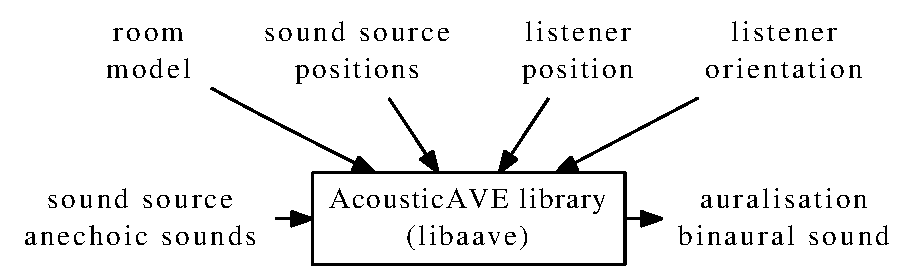
\includegraphics{libaave}
\caption{Role of the Acoustic\-A\-V\-E library}
\end{DoxyImage}
 libaave supports moving sound sources and listener, therefore it can be used for auralisation of interactive virtual reality environments, usually in combination with a 3\-D graphics visualisation library.

libaave performs in real-\/time for virtual rooms of some complexity (number of surfaces) and some order of sound reflections (configured by the user), more specifically the total number of sounds, that depend on the processor used. Benchmarks\-:
\begin{DoxyItemize}
\item Intel Atom N2600 1.\-6\-G\-Hz\-: 66 sounds
\item Intel Xeon 2\-G\-Hz\-: 89 sounds
\item A\-M\-D Opteron 248 2.\-2\-G\-Hz\-: 193 sounds
\end{DoxyItemize}

The following diagrams illustrate typical usages of the Acoustic\-A\-V\-E library for developing auralisation programs, one single-\/threaded and one multi-\/threaded.


\begin{DoxyImage}
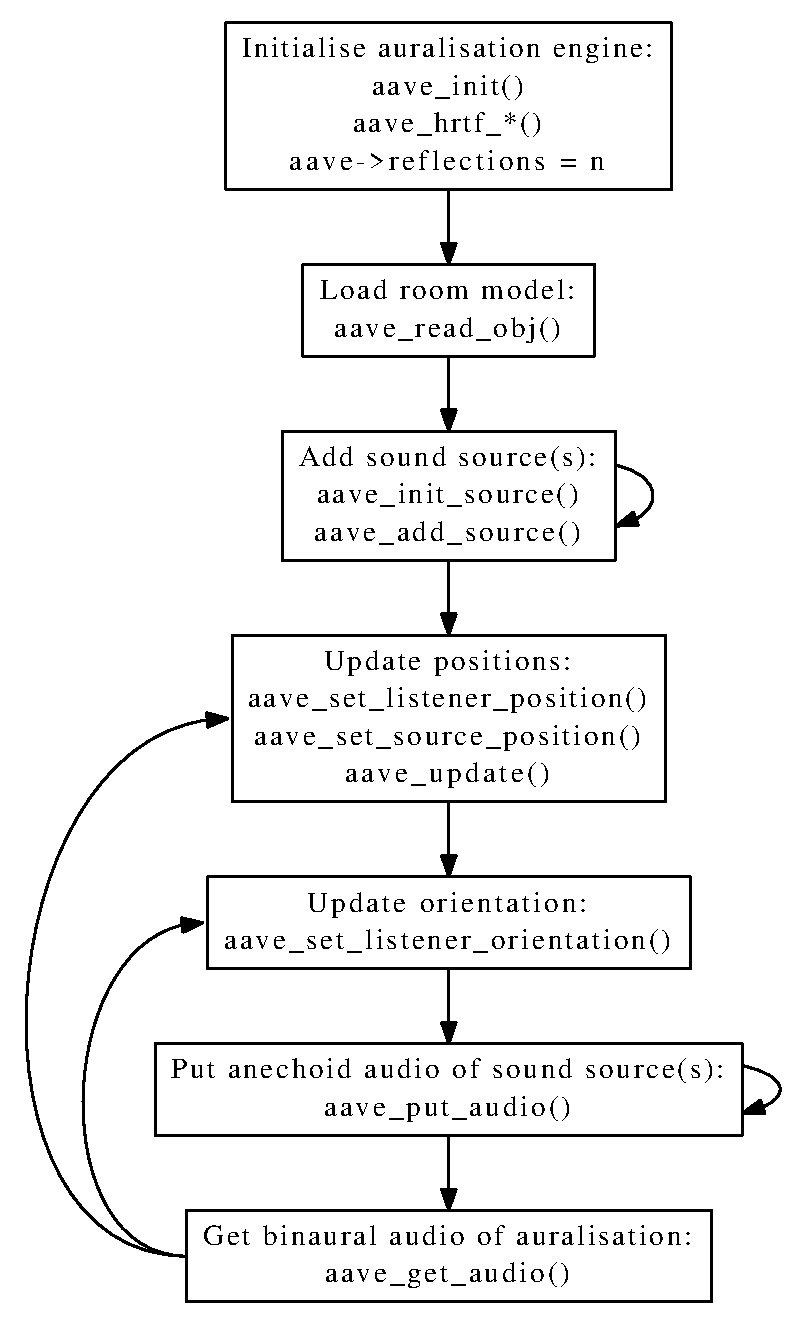
\includegraphics{usage1}
\caption{Single-\/thread usage example}
\end{DoxyImage}
 
\begin{DoxyImage}
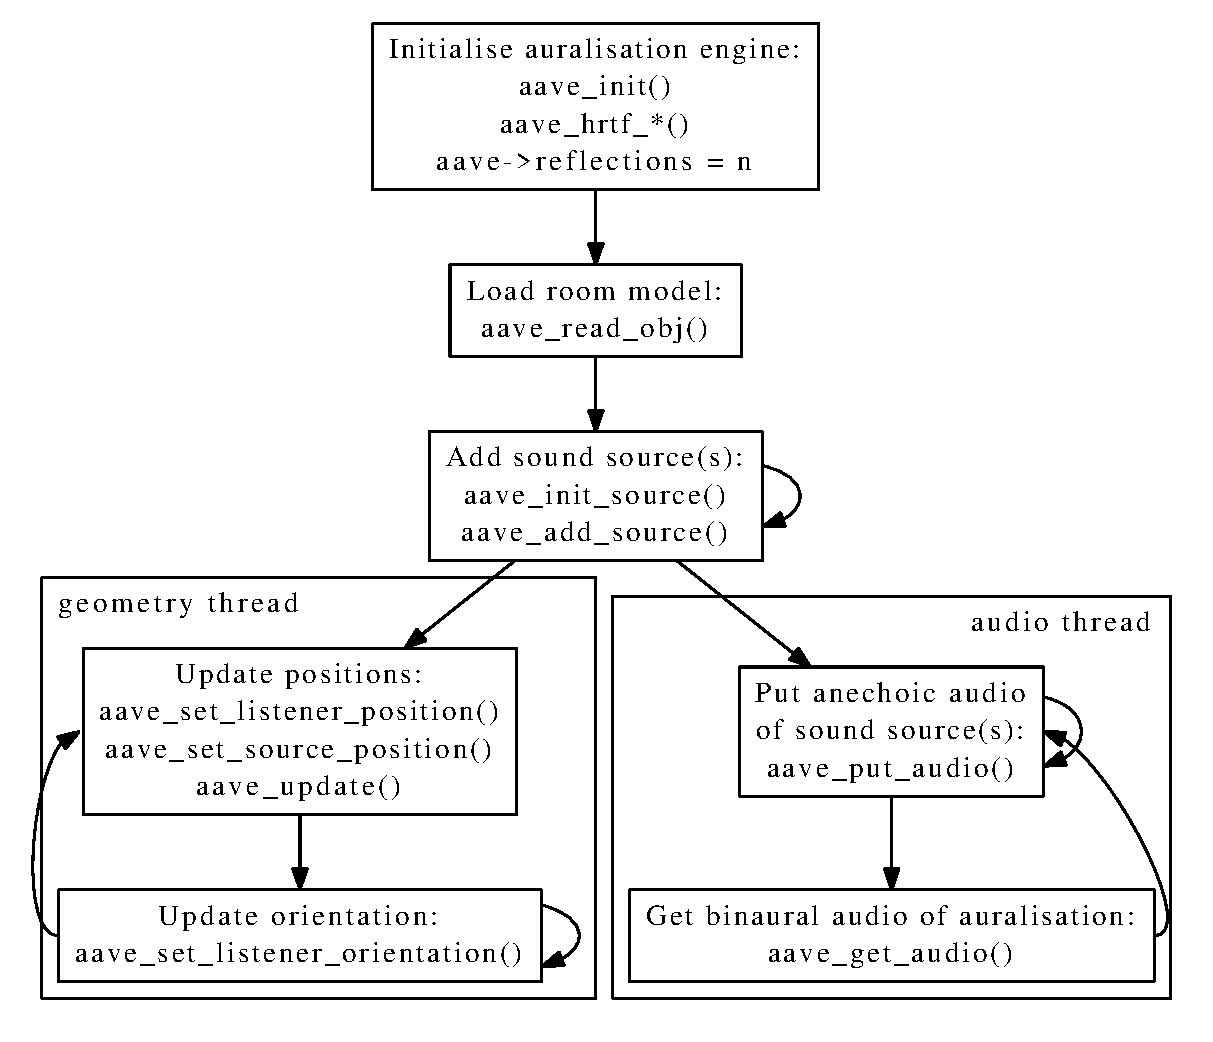
\includegraphics[width=\textwidth]{usage2}
\caption{Multi-\/thread usage example}
\end{DoxyImage}
\hypertarget{index_installation}{}\section{Installation}\label{index_installation}
libaave is implemented in A\-N\-S\-I C and does not depend on any external library, so it is fairly portable (it is known to work on G\-N\-U/\-Linux and Microsoft Windows systems, but should also work on any other platform with an A\-N\-S\-I C compiler).
\begin{DoxyEnumerate}
\item Download the source code\-: 
\begin{DoxyCode}
git clone https:\textcolor{comment}{//code.ua.pt/git/acousticave}
\end{DoxyCode}

\item Build libaave\-: 
\begin{DoxyCode}
cd acousticave/libaave
make
\end{DoxyCode}

\end{DoxyEnumerate}

For a quick start on using libaave in your programs, see the examples in acousticave/libaave/examples/.\hypertarget{index_coordinates}{}\section{Coordinates}\label{index_coordinates}
For all 3\-D points (positions and room model vertices), libaave uses the coordinate system commonly used by C\-A\-D architecture programs\-: x=North, y=West, z=up, in metres.

For the listener head orientation angles, libaave uses the coordinate system commonly used by inertial sensors\-: x=North, y=East, z=down, in radians. This means\-:
\begin{DoxyItemize}
\item roll $>$ 0 is tilt right, roll $<$ 0 is tilt left
\item pitch $>$ 0 is tilt up, pitch $<$ 0 is tilt down
\item yaw $>$ 0 is rotate right, yaw $<$ 0 is rotate left, yaw = 0 is North
\end{DoxyItemize}\hypertarget{index_overview}{}\section{Overview}\label{index_overview}
The file \hyperlink{aave_8h}{aave.\-h} is the public header file of libaave. Include it from your program source files to use its structures and functions.

The file \hyperlink{geometry_8c}{geometry.\-c} implements all functions related to geometry processing\-: construction of the 3\-D room model, coordinate conversions, determining the image-\/source positions, the sound reflection paths, the audible and non-\/audible sound paths, and passing all this information to the audio processing functions.

The file \hyperlink{obj_8c}{obj.\-c} contains a convenience function that reads a 3\-D model from a Wavefront .O\-B\-J file and calls the appropriate functions in \hyperlink{geometry_8c}{geometry.\-c} to construct the room to be auralised in just one step.

The file \hyperlink{audio_8c}{audio.\-c} implements the core of the audio processing\-: receiving anechoic audio data from the sound sources, head-\/related transfer function (H\-R\-T\-F) processing, and generating the corresponding auralised audio data in binaural format.

The files \hyperlink{hrtf__cipic_8c}{hrtf\-\_\-cipic.\-c}, \hyperlink{hrtf__listen_8c}{hrtf\-\_\-listen.\-c}, \hyperlink{hrtf__mit_8c}{hrtf\-\_\-mit.\-c}, and \hyperlink{hrtf__tub_8c}{hrtf\-\_\-tub.\-c} implement the interface functions for using the C\-I\-P\-I\-C, L\-I\-S\-T\-E\-N, M\-I\-T, and T\-U-\/\-Berlin H\-R\-T\-F sets, respectively.

The files \hyperlink{dft_8h}{dft.\-h} and \hyperlink{idft_8h}{idft.\-h} implement the Discrete Fourier Transform and Inverse Discrete Fourier Transform algorithms, respectively, used mainly for the H\-R\-T\-F processing.

The file \hyperlink{material_8c}{material.\-c} implements the functions related to the sound absorption caused by the different surface materials\-: the table of material reflection coefficients by frequency band, the table lookup, and the design of the audio filters.

The file reverb.\-c implements a simple artificial reverberation algorithm that adds a tail of late reflections to the auralisation output. The file \hyperlink{reverb__dattorro_8c}{reverb\-\_\-dattorro.\-c} implements the Dattorro reverberator.

The directory tools contains the programs used to automatically generate the hrtf\-\_\-$\ast$\-\_\-set$\ast$.c source files from the respective H\-R\-T\-F data sets, the dftsincos.\-c source file with the sin() and cos() lookup table for the D\-F\-T and I\-D\-F\-T algorithms, and miscellaneous utility programs to handle or generate audio files.

The directory tests/ contains programs to verify the correctness of the functions implemented in libaave.

The directory examples/ contains programs to show how libaave can be used for different auralisation applications.

The directory doc/ contains the files to generate this document from the documentation written in the source files.\hypertarget{index_acknowledgements}{}\section{Acknowledgements}\label{index_acknowledgements}
The development of libaave was funded by the Portuguese Government through F\-C\-T (Fundação para a Ciência e a Tecnologia) as part of the project Acoustic\-A\-V\-E\-: Auralisation Models and Applications for Virtual Reality Environments (P\-T\-D\-C/\-E\-E\-A-\/\-E\-L\-C/112137/2009). 
\chapter{Todo List}
\label{todo}
\hypertarget{todo}{}

\begin{DoxyRefList}
\item[\label{todo__todo000007}%
\hypertarget{todo__todo000007}{}%
Global \hyperlink{geometry_8c_a2c55d6e06ff73570a887d18807442412}{aave\-\_\-create\-\_\-sounds\-\_\-recursively} (struct aave $\ast$aave, struct \hyperlink{structaave__source}{aave\-\_\-source} $\ast$source, unsigned order, unsigned o, struct \hyperlink{structaave__surface}{aave\-\_\-surface} $\ast$surfaces\mbox{[}\mbox{]}, float image\-\_\-sources\mbox{[}\mbox{]}\mbox{[}3\mbox{]})]Implement the iterative version of this recursive algorithm.  
\item[\label{todo__todo000001}%
\hypertarget{todo__todo000001}{}%
Global \hyperlink{aave_8h_aff6fdc3178c7698a824bf53f79d0bdd1}{A\-A\-V\-E\-\_\-\-F\-S} ]To support different audio sampling frequencies without having to recompile the library, this value would be set in a member of the aave structure at runtime instead. Of course, that would incur in performance penalties, most importantly in the audio processing (one floating-\/point division per audio sample per auralised sound). Furthermore, the H\-R\-T\-F data sets would have to be resampled to the desired sampling frequency.  
\item[\label{todo__todo000008}%
\hypertarget{todo__todo000008}{}%
Global \hyperlink{hrtf__cipic_8c_a4b3a15263cf86760cf69027db5aab73a}{aave\-\_\-hrtf\-\_\-cipic\-\_\-get} (const float $\ast$hrtf\mbox{[}2\mbox{]}, int elevation, int azimuth)]Use all elevation measures available, not just 0 degrees.  
\item[\label{todo__todo000009}%
\hypertarget{todo__todo000009}{}%
Global \hyperlink{hrtf__listen_8c_a3239bc0a4a965c5da5334695d4f39c06}{aave\-\_\-hrtf\-\_\-listen\-\_\-get} (const float $\ast$hrtf\mbox{[}2\mbox{]}, int elevation, int azimuth)]Elevations 60, 75 and 90.  
\item[\label{todo__todo000003}%
\hypertarget{todo__todo000003}{}%
Global \hyperlink{aave_8h_a19ea3a18eb313fc3b825f522245d19d3}{A\-A\-V\-E\-\_\-\-M\-A\-X\-\_\-\-H\-R\-T\-F} ]When using H\-R\-T\-Fs with less frames (M\-I\-T only has 128) there is a considerable waste of memory throughout the library. However, this way the code is much simpler, and slightly faster. Nevertheless, it would be nice if this value could be changed at runtime when the user selects the H\-R\-T\-F set to use.  
\item[\label{todo__todo000002}%
\hypertarget{todo__todo000002}{}%
Global \hyperlink{aave_8h_a5cc7807cca10cf0933038ad388171181}{A\-A\-V\-E\-\_\-\-M\-A\-X\-\_\-\-R\-E\-F\-L\-E\-C\-T\-I\-O\-N\-S} ]To support different maximum orders of reflections per instance, this value would be set in a member of the aave structure at runtime and the sounds hash table allocated accordingly. However, I think this is not worth the trouble. Just change this value and recompile, if you want more orders of reflections (and your computer can handle them). The waste is only 4 or 8 bytes per reflection order that is not used, for 32-\/bit or 64-\/bit processors respectively.  
\item[\label{todo__todo000004}%
\hypertarget{todo__todo000004}{}%
Global \hyperlink{structaave__surface_a6bd0e3127c052c7cf3ffa49480acda83}{aave\-\_\-surface\-:\-:points} \mbox{[}32\mbox{]}\mbox{[}3+2\mbox{]}]Remove hardcoded maximum number of points per surface.  
\item[\label{todo__todo000013}%
\hypertarget{todo__todo000013}{}%
Global \hyperlink{reverb__dattorro_8c_a63533538546edde6ae7f3c88192ae6a3}{allpass} (struct allpass $\ast$ap, float x, float g, unsigned delay)]Check if the tap is really x1 or x2.  
\item[\label{todo__todo000015}%
\hypertarget{todo__todo000015}{}%
Global \hyperlink{structallpass_a9a88e7125eb10d734a1a408c26cebe49}{allpass\-:\-:buffer} \mbox{[}2656\mbox{]}]Set maximum delay from the delays of all all-\/pass blocks.  
\item[\label{todo__todo000005}%
\hypertarget{todo__todo000005}{}%
File \hyperlink{audio_8c}{audio.c} ]Here, it might be more efficient to use the overlap-\/save method instead of the overlap-\/add method. 
\item[\label{todo__todo000017}%
\hypertarget{todo__todo000017}{}%
Class \hyperlink{structdc__block__filter}{dc\-\_\-block\-\_\-filter} ]Improve bandwidth definition.  
\item[\label{todo__todo000014}%
\hypertarget{todo__todo000014}{}%
Global \hyperlink{structdelay_a655d8b9f8d1bcd90764042b7e6e58ea7}{delay\-:\-:buffer} \mbox{[}16384\mbox{]}]Set maximum delay from the delays of all delay blocks.  
\item[\label{todo__todo000006}%
\hypertarget{todo__todo000006}{}%
Global \hyperlink{dftindex_8c_ad9fc4c6b2778357224f5341cf268f78c}{dft\-\_\-index\-\_\-table} \mbox{[}\mbox{]}]If the order of the material absorption filter designed in \hyperlink{material_8c}{material.\-c} increases to N $>$ 128, increase this table accordingly.  
\item[\label{todo__todo000010}%
\hypertarget{todo__todo000010}{}%
Global \hyperlink{idft_8h_a797484e3f3d53d566ececbcfcd90f537}{idft} (I\-D\-F\-T\-\_\-\-T\-Y\-P\-E $\ast$x, float $\ast$\-X, unsigned n)]round instead of truncate  
\item[\label{todo__todo000011}%
\hypertarget{todo__todo000011}{}%
Global \hyperlink{obj_8c_a0fdb7b933ef091574ff57d1f36dd4167}{M\-A\-X\-\_\-\-V\-E\-R\-T\-I\-C\-E\-S} ]Use dynamic memory allocation for the array of vertices to support \char`\"{}unlimited\char`\"{} number of vertices.  
\item[\label{todo__todo000012}%
\hypertarget{todo__todo000012}{}%
File \hyperlink{reverb__dattorro_8c}{reverb\-\_\-dattorro.c} ]Make the code reentrant (move the static structures to aave). 
\item[\label{todo__todo000016}%
\hypertarget{todo__todo000016}{}%
File \hyperlink{reverb__jot_8c}{reverb\-\_\-jot.c} ]A {\ttfamily \hyperlink{structdc__block__filter}{dc\-\_\-block\-\_\-filter}} was introduced to aproximate low frequency damping. Improve this filter (or introduce another) for flexible bandwidth selection. 
\end{DoxyRefList}
\chapter{Data Structure Index}
\section{Data Structures}
Here are the data structures with brief descriptions\-:\begin{DoxyCompactList}
\item\contentsline{section}{\hyperlink{structaave}{aave} }{\pageref{structaave}}{}
\item\contentsline{section}{\hyperlink{structaave__material}{aave\-\_\-material} }{\pageref{structaave__material}}{}
\item\contentsline{section}{\hyperlink{structaave__reverb}{aave\-\_\-reverb} }{\pageref{structaave__reverb}}{}
\item\contentsline{section}{\hyperlink{structaave__sound}{aave\-\_\-sound} }{\pageref{structaave__sound}}{}
\item\contentsline{section}{\hyperlink{structaave__source}{aave\-\_\-source} }{\pageref{structaave__source}}{}
\item\contentsline{section}{\hyperlink{structaave__surface}{aave\-\_\-surface} }{\pageref{structaave__surface}}{}
\item\contentsline{section}{\hyperlink{structabsorption__filter}{absorption\-\_\-filter} }{\pageref{structabsorption__filter}}{}
\item\contentsline{section}{\hyperlink{structallpass}{allpass} }{\pageref{structallpass}}{}
\item\contentsline{section}{\hyperlink{structdc__block__filter}{dc\-\_\-block\-\_\-filter} }{\pageref{structdc__block__filter}}{}
\item\contentsline{section}{\hyperlink{structdecay__block}{decay\-\_\-block} }{\pageref{structdecay__block}}{}
\item\contentsline{section}{\hyperlink{structdelay}{delay} }{\pageref{structdelay}}{}
\item\contentsline{section}{\hyperlink{structdelay__filter}{delay\-\_\-filter} }{\pageref{structdelay__filter}}{}
\item\contentsline{section}{\hyperlink{structlowpass}{lowpass} }{\pageref{structlowpass}}{}
\item\contentsline{section}{\hyperlink{structtone__correction__filter}{tone\-\_\-correction\-\_\-filter} }{\pageref{structtone__correction__filter}}{}
\end{DoxyCompactList}

\chapter{File Index}
\section{File List}
Here is a list of all documented files with brief descriptions\-:\begin{DoxyCompactList}
\item\contentsline{section}{\hyperlink{aave_8h}{aave.\-h} }{\pageref{aave_8h}}{}
\item\contentsline{section}{\hyperlink{audio_8c}{audio.\-c} }{\pageref{audio_8c}}{}
\item\contentsline{section}{\hyperlink{dft_8h}{dft.\-h} }{\pageref{dft_8h}}{}
\item\contentsline{section}{\hyperlink{dftindex_8c}{dftindex.\-c} }{\pageref{dftindex_8c}}{}
\item\contentsline{section}{\hyperlink{geometry_8c}{geometry.\-c} }{\pageref{geometry_8c}}{}
\item\contentsline{section}{\hyperlink{hrtf__cipic_8c}{hrtf\-\_\-cipic.\-c} }{\pageref{hrtf__cipic_8c}}{}
\item\contentsline{section}{\hyperlink{hrtf__listen_8c}{hrtf\-\_\-listen.\-c} }{\pageref{hrtf__listen_8c}}{}
\item\contentsline{section}{\hyperlink{hrtf__mit_8c}{hrtf\-\_\-mit.\-c} }{\pageref{hrtf__mit_8c}}{}
\item\contentsline{section}{\hyperlink{hrtf__tub_8c}{hrtf\-\_\-tub.\-c} }{\pageref{hrtf__tub_8c}}{}
\item\contentsline{section}{\hyperlink{idft_8h}{idft.\-h} }{\pageref{idft_8h}}{}
\item\contentsline{section}{\hyperlink{init_8c}{init.\-c} }{\pageref{init_8c}}{}
\item\contentsline{section}{\hyperlink{material_8c}{material.\-c} }{\pageref{material_8c}}{}
\item\contentsline{section}{\hyperlink{obj_8c}{obj.\-c} }{\pageref{obj_8c}}{}
\item\contentsline{section}{\hyperlink{reverb__dattorro_8c}{reverb\-\_\-dattorro.\-c} }{\pageref{reverb__dattorro_8c}}{}
\item\contentsline{section}{\hyperlink{reverb__jot_8c}{reverb\-\_\-jot.\-c} }{\pageref{reverb__jot_8c}}{}
\end{DoxyCompactList}

\chapter{Data Structure Documentation}
\hypertarget{structaave}{\section{aave Struct Reference}
\label{structaave}\index{aave@{aave}}
}


{\ttfamily \#include $<$aave.\-h$>$}



Collaboration diagram for aave\-:\nopagebreak
\begin{figure}[H]
\begin{center}
\leavevmode
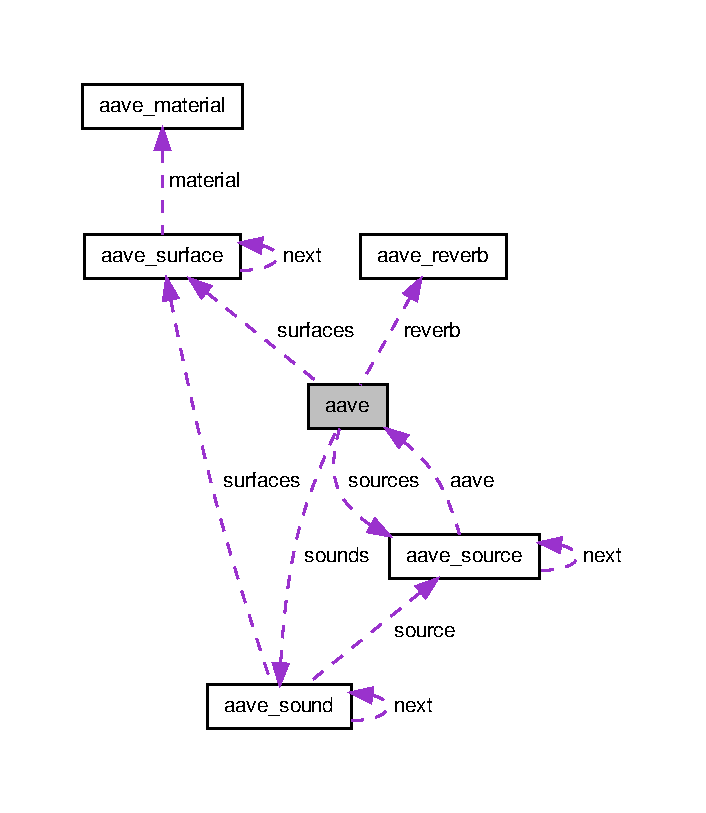
\includegraphics[width=339pt]{structaave__coll__graph}
\end{center}
\end{figure}
\subsection*{Data Fields}
\begin{DoxyCompactItemize}
\item 
float \hyperlink{structaave_aa592d293dfb41b86d48c0529fd3549d6}{position} \mbox{[}3\mbox{]}
\item 
float \hyperlink{structaave_a1380ca0c5d7610cf1b409043b93b2680}{orientation} \mbox{[}3\mbox{]}\mbox{[}3\mbox{]}
\item 
struct \hyperlink{structaave__surface}{aave\-\_\-surface} $\ast$ \hyperlink{structaave_ad7a69df05d26827f132c742551fb8871}{surfaces}
\item 
unsigned \hyperlink{structaave_a46897bdef9912d50cecb6b93c8c894a6}{nsurfaces}
\item 
float \hyperlink{structaave_afe632929215cd44b7344bb4380df1c69}{room\-\_\-material\-\_\-absorption}
\item 
unsigned \hyperlink{structaave_a6d16180d7cb50c0255180a0102abfc2e}{volume}
\item 
unsigned \hyperlink{structaave_ad7a37d4250667623a1cd209b5aa421dd}{area}
\item 
struct \hyperlink{structaave__source}{aave\-\_\-source} $\ast$ \hyperlink{structaave_ad6f8dfdcb3403e1cf8e8b42c16851317}{sources}
\item 
struct \hyperlink{structaave__sound}{aave\-\_\-sound} $\ast$ \hyperlink{structaave_aa637fd7286c95ab8322e391f461e825d}{sounds} \mbox{[}\hyperlink{aave_8h_a5cc7807cca10cf0933038ad388171181}{A\-A\-V\-E\-\_\-\-M\-A\-X\-\_\-\-R\-E\-F\-L\-E\-C\-T\-I\-O\-N\-S}\mbox{]}
\item 
unsigned \hyperlink{structaave_a89d048be9cbd805d11b23d0c8d118eb8}{reflections}
\item 
struct \hyperlink{structaave__reverb}{aave\-\_\-reverb} $\ast$ \hyperlink{structaave_ad2e95c7026a1361aebbd89107903c4be}{reverb}
\item 
float \hyperlink{structaave_a8cb46909713b403fa7f54b75dee1e81f}{gain}
\item 
unsigned \hyperlink{structaave_a41b7518a03a90f29e627adf308e68200}{hrtf\-\_\-frames}
\item 
void($\ast$ \hyperlink{structaave_a5ab930083fffbd9efe3bffe51dae585b}{hrtf\-\_\-get} )(const float $\ast$hrtf\mbox{[}2\mbox{]}, int elevation, int azimuth)
\item 
unsigned \hyperlink{structaave_a50881090e68ae1bde54b091757b99d64}{hrtf\-\_\-output\-\_\-buffer\-\_\-index}
\item 
short \hyperlink{structaave_a4aabeeaaa2fd6eecaa74cf9ff6a4a75c}{hrtf\-\_\-output\-\_\-buffer} \mbox{[}\hyperlink{aave_8h_a19ea3a18eb313fc3b825f522245d19d3}{A\-A\-V\-E\-\_\-\-M\-A\-X\-\_\-\-H\-R\-T\-F} $\ast$4\mbox{]}
\item 
int \hyperlink{structaave_a591c8877020f861da25632f35f67c3b4}{hrtf\-\_\-overlap\-\_\-add\-\_\-buffer} \mbox{[}2\mbox{]}\mbox{[}\hyperlink{aave_8h_a19ea3a18eb313fc3b825f522245d19d3}{A\-A\-V\-E\-\_\-\-M\-A\-X\-\_\-\-H\-R\-T\-F} $\ast$2\mbox{]}
\end{DoxyCompactItemize}


\subsection{Detailed Description}
The Acoustic\-A\-V\-E main data structure. It contains all the information that defines one acoustic world and its present auralisation state. \begin{Desc}
\item[Examples\-: ]\par
\hyperlink{examples_2circle_8c-example}{examples/circle.\-c}, \hyperlink{examples_2elevation_8c-example}{examples/elevation.\-c}, \hyperlink{examples_2line_8c-example}{examples/line.\-c}, and \hyperlink{examples_2stream_8c-example}{examples/stream.\-c}.\end{Desc}


\subsection{Field Documentation}
\hypertarget{structaave_ad7a37d4250667623a1cd209b5aa421dd}{\index{aave@{aave}!area@{area}}
\index{area@{area}!aave@{aave}}
\subsubsection[{area}]{\setlength{\rightskip}{0pt plus 5cm}unsigned aave\-::area}}\label{structaave_ad7a37d4250667623a1cd209b5aa421dd}
Sum of all room surface areas. \hypertarget{structaave_a8cb46909713b403fa7f54b75dee1e81f}{\index{aave@{aave}!gain@{gain}}
\index{gain@{gain}!aave@{aave}}
\subsubsection[{gain}]{\setlength{\rightskip}{0pt plus 5cm}float aave\-::gain}}\label{structaave_a8cb46909713b403fa7f54b75dee1e81f}
Gain to apply to the output sound. \hypertarget{structaave_a41b7518a03a90f29e627adf308e68200}{\index{aave@{aave}!hrtf\-\_\-frames@{hrtf\-\_\-frames}}
\index{hrtf\-\_\-frames@{hrtf\-\_\-frames}!aave@{aave}}
\subsubsection[{hrtf\-\_\-frames}]{\setlength{\rightskip}{0pt plus 5cm}unsigned aave\-::hrtf\-\_\-frames}}\label{structaave_a41b7518a03a90f29e627adf308e68200}
The number of frames of the H\-R\-T\-Fs currently in use (power of 2). \hypertarget{structaave_a5ab930083fffbd9efe3bffe51dae585b}{\index{aave@{aave}!hrtf\-\_\-get@{hrtf\-\_\-get}}
\index{hrtf\-\_\-get@{hrtf\-\_\-get}!aave@{aave}}
\subsubsection[{hrtf\-\_\-get}]{\setlength{\rightskip}{0pt plus 5cm}void($\ast$ aave\-::hrtf\-\_\-get)(const float $\ast$hrtf\mbox{[}2\mbox{]}, int elevation, int azimuth)}}\label{structaave_a5ab930083fffbd9efe3bffe51dae585b}
Function to get the H\-R\-T\-F pair for some elevation and azimuth. \hypertarget{structaave_a4aabeeaaa2fd6eecaa74cf9ff6a4a75c}{\index{aave@{aave}!hrtf\-\_\-output\-\_\-buffer@{hrtf\-\_\-output\-\_\-buffer}}
\index{hrtf\-\_\-output\-\_\-buffer@{hrtf\-\_\-output\-\_\-buffer}!aave@{aave}}
\subsubsection[{hrtf\-\_\-output\-\_\-buffer}]{\setlength{\rightskip}{0pt plus 5cm}short aave\-::hrtf\-\_\-output\-\_\-buffer\mbox{[}{\bf A\-A\-V\-E\-\_\-\-M\-A\-X\-\_\-\-H\-R\-T\-F} $\ast$4\mbox{]}}}\label{structaave_a4aabeeaaa2fd6eecaa74cf9ff6a4a75c}
H\-R\-T\-F audio block output buffer (2 16-\/bit channels interleaved). \hypertarget{structaave_a50881090e68ae1bde54b091757b99d64}{\index{aave@{aave}!hrtf\-\_\-output\-\_\-buffer\-\_\-index@{hrtf\-\_\-output\-\_\-buffer\-\_\-index}}
\index{hrtf\-\_\-output\-\_\-buffer\-\_\-index@{hrtf\-\_\-output\-\_\-buffer\-\_\-index}!aave@{aave}}
\subsubsection[{hrtf\-\_\-output\-\_\-buffer\-\_\-index}]{\setlength{\rightskip}{0pt plus 5cm}unsigned aave\-::hrtf\-\_\-output\-\_\-buffer\-\_\-index}}\label{structaave_a50881090e68ae1bde54b091757b99d64}
Index of the next frame of the H\-R\-T\-F output buffer to be consumed. \hypertarget{structaave_a591c8877020f861da25632f35f67c3b4}{\index{aave@{aave}!hrtf\-\_\-overlap\-\_\-add\-\_\-buffer@{hrtf\-\_\-overlap\-\_\-add\-\_\-buffer}}
\index{hrtf\-\_\-overlap\-\_\-add\-\_\-buffer@{hrtf\-\_\-overlap\-\_\-add\-\_\-buffer}!aave@{aave}}
\subsubsection[{hrtf\-\_\-overlap\-\_\-add\-\_\-buffer}]{\setlength{\rightskip}{0pt plus 5cm}int aave\-::hrtf\-\_\-overlap\-\_\-add\-\_\-buffer\mbox{[}2\mbox{]}\mbox{[}{\bf A\-A\-V\-E\-\_\-\-M\-A\-X\-\_\-\-H\-R\-T\-F} $\ast$2\mbox{]}}}\label{structaave_a591c8877020f861da25632f35f67c3b4}
H\-R\-T\-F overlap-\/add buffer (2 32-\/bit channels). \hypertarget{structaave_a46897bdef9912d50cecb6b93c8c894a6}{\index{aave@{aave}!nsurfaces@{nsurfaces}}
\index{nsurfaces@{nsurfaces}!aave@{aave}}
\subsubsection[{nsurfaces}]{\setlength{\rightskip}{0pt plus 5cm}unsigned aave\-::nsurfaces}}\label{structaave_a46897bdef9912d50cecb6b93c8c894a6}
Number of surfaces in the list of surfaces. \hypertarget{structaave_a1380ca0c5d7610cf1b409043b93b2680}{\index{aave@{aave}!orientation@{orientation}}
\index{orientation@{orientation}!aave@{aave}}
\subsubsection[{orientation}]{\setlength{\rightskip}{0pt plus 5cm}float aave\-::orientation\mbox{[}3\mbox{]}\mbox{[}3\mbox{]}}}\label{structaave_a1380ca0c5d7610cf1b409043b93b2680}
Listener head orientation (inertial-\/to-\/body rotation matrix). \hypertarget{structaave_aa592d293dfb41b86d48c0529fd3549d6}{\index{aave@{aave}!position@{position}}
\index{position@{position}!aave@{aave}}
\subsubsection[{position}]{\setlength{\rightskip}{0pt plus 5cm}float aave\-::position\mbox{[}3\mbox{]}}}\label{structaave_aa592d293dfb41b86d48c0529fd3549d6}
Position of the listener in the auralization world \mbox{[}x,y,z\mbox{]} (m). \hypertarget{structaave_a89d048be9cbd805d11b23d0c8d118eb8}{\index{aave@{aave}!reflections@{reflections}}
\index{reflections@{reflections}!aave@{aave}}
\subsubsection[{reflections}]{\setlength{\rightskip}{0pt plus 5cm}unsigned aave\-::reflections}}\label{structaave_a89d048be9cbd805d11b23d0c8d118eb8}
Maximum number of reflections to calculate for each source. \begin{Desc}
\item[Examples\-: ]\par
\hyperlink{examples_2stream_8c-example}{examples/stream.\-c}.\end{Desc}
\hypertarget{structaave_ad2e95c7026a1361aebbd89107903c4be}{\index{aave@{aave}!reverb@{reverb}}
\index{reverb@{reverb}!aave@{aave}}
\subsubsection[{reverb}]{\setlength{\rightskip}{0pt plus 5cm}struct {\bf aave\-\_\-reverb}$\ast$ aave\-::reverb}}\label{structaave_ad2e95c7026a1361aebbd89107903c4be}
Late reverberation parameters. \hypertarget{structaave_afe632929215cd44b7344bb4380df1c69}{\index{aave@{aave}!room\-\_\-material\-\_\-absorption@{room\-\_\-material\-\_\-absorption}}
\index{room\-\_\-material\-\_\-absorption@{room\-\_\-material\-\_\-absorption}!aave@{aave}}
\subsubsection[{room\-\_\-material\-\_\-absorption}]{\setlength{\rightskip}{0pt plus 5cm}float aave\-::room\-\_\-material\-\_\-absorption}}\label{structaave_afe632929215cd44b7344bb4380df1c69}
Average of all room surface absorption coeficients. \hypertarget{structaave_aa637fd7286c95ab8322e391f461e825d}{\index{aave@{aave}!sounds@{sounds}}
\index{sounds@{sounds}!aave@{aave}}
\subsubsection[{sounds}]{\setlength{\rightskip}{0pt plus 5cm}struct {\bf aave\-\_\-sound}$\ast$ aave\-::sounds\mbox{[}{\bf A\-A\-V\-E\-\_\-\-M\-A\-X\-\_\-\-R\-E\-F\-L\-E\-C\-T\-I\-O\-N\-S}\mbox{]}}}\label{structaave_aa637fd7286c95ab8322e391f461e825d}
Hash table of sounds to auralise, indexed by reflection order. \hypertarget{structaave_ad6f8dfdcb3403e1cf8e8b42c16851317}{\index{aave@{aave}!sources@{sources}}
\index{sources@{sources}!aave@{aave}}
\subsubsection[{sources}]{\setlength{\rightskip}{0pt plus 5cm}struct {\bf aave\-\_\-source}$\ast$ aave\-::sources}}\label{structaave_ad6f8dfdcb3403e1cf8e8b42c16851317}
Singly-\/linked list of sound sources in the auralisation world. \hypertarget{structaave_ad7a69df05d26827f132c742551fb8871}{\index{aave@{aave}!surfaces@{surfaces}}
\index{surfaces@{surfaces}!aave@{aave}}
\subsubsection[{surfaces}]{\setlength{\rightskip}{0pt plus 5cm}struct {\bf aave\-\_\-surface}$\ast$ aave\-::surfaces}}\label{structaave_ad7a69df05d26827f132c742551fb8871}
Singly-\/linked list of surfaces in the auralisation world. \hypertarget{structaave_a6d16180d7cb50c0255180a0102abfc2e}{\index{aave@{aave}!volume@{volume}}
\index{volume@{volume}!aave@{aave}}
\subsubsection[{volume}]{\setlength{\rightskip}{0pt plus 5cm}unsigned aave\-::volume}}\label{structaave_a6d16180d7cb50c0255180a0102abfc2e}
Room volume (m3). 

The documentation for this struct was generated from the following file\-:\begin{DoxyCompactItemize}
\item 
\hyperlink{aave_8h}{aave.\-h}\end{DoxyCompactItemize}

\hypertarget{structaave__material}{\section{aave\-\_\-material Struct Reference}
\label{structaave__material}\index{aave\-\_\-material@{aave\-\_\-material}}
}


{\ttfamily \#include $<$aave.\-h$>$}

\subsection*{Data Fields}
\begin{DoxyCompactItemize}
\item 
const char $\ast$ \hyperlink{structaave__material_af0ba4eaedad26368f33bba9eecddf77a}{name}
\item 
const unsigned char \hyperlink{structaave__material_a8a90deb71af157f83779e7b8d8d4a00f}{reflection\-\_\-factors} \mbox{[}\hyperlink{aave_8h_ad76f6ee2a275c27185c10ff7ea5187b2}{A\-A\-V\-E\-\_\-\-M\-A\-T\-E\-R\-I\-A\-L\-\_\-\-R\-E\-F\-L\-E\-C\-T\-I\-O\-N\-\_\-\-F\-A\-C\-T\-O\-R\-S}\mbox{]}
\end{DoxyCompactItemize}


\subsection{Detailed Description}
Acoustic properties of a material. 

\subsection{Field Documentation}
\hypertarget{structaave__material_af0ba4eaedad26368f33bba9eecddf77a}{\index{aave\-\_\-material@{aave\-\_\-material}!name@{name}}
\index{name@{name}!aave_material@{aave\-\_\-material}}
\subsubsection[{name}]{\setlength{\rightskip}{0pt plus 5cm}const char$\ast$ aave\-\_\-material\-::name}}\label{structaave__material_af0ba4eaedad26368f33bba9eecddf77a}
Name used in the usemtl directives of the .obj files. \hypertarget{structaave__material_a8a90deb71af157f83779e7b8d8d4a00f}{\index{aave\-\_\-material@{aave\-\_\-material}!reflection\-\_\-factors@{reflection\-\_\-factors}}
\index{reflection\-\_\-factors@{reflection\-\_\-factors}!aave_material@{aave\-\_\-material}}
\subsubsection[{reflection\-\_\-factors}]{\setlength{\rightskip}{0pt plus 5cm}const unsigned char aave\-\_\-material\-::reflection\-\_\-factors\mbox{[}{\bf A\-A\-V\-E\-\_\-\-M\-A\-T\-E\-R\-I\-A\-L\-\_\-\-R\-E\-F\-L\-E\-C\-T\-I\-O\-N\-\_\-\-F\-A\-C\-T\-O\-R\-S}\mbox{]}}}\label{structaave__material_a8a90deb71af157f83779e7b8d8d4a00f}
Reflection factors (multiplied by 100), by frequency band. 

The documentation for this struct was generated from the following file\-:\begin{DoxyCompactItemize}
\item 
\hyperlink{aave_8h}{aave.\-h}\end{DoxyCompactItemize}

\hypertarget{structaave__reverb}{\section{aave\-\_\-reverb Struct Reference}
\label{structaave__reverb}\index{aave\-\_\-reverb@{aave\-\_\-reverb}}
}
\subsection*{Data Fields}
\begin{DoxyCompactItemize}
\item 
unsigned \hyperlink{structaave__reverb_a61f593c67c5e0ac18c2255c3c0830bc1}{R\-T60}
\item 
float \hyperlink{structaave__reverb_aa650231c06910bb5e352682b1bd6bd19}{Tmixing}
\item 
float \hyperlink{structaave__reverb_a2bc62b21b9ba27d56575f7ddbf23ff89}{rc}
\item 
float \hyperlink{structaave__reverb_a338401b5113dcb382637d43dba5f4aa5}{pre\-\_\-delay}
\item 
float \hyperlink{structaave__reverb_a797c24d78e79d4a3bfec25e5a625dc46}{alpha}
\item 
short \hyperlink{structaave__reverb_a2e40ddc7cc824ddf535c1e80fb1145d5}{decorrelation\-\_\-coefs} \mbox{[}\hyperlink{aave_8h_aa8ac0978ba9be33dd450abaaa2dda4d9}{F\-D\-N\-\_\-\-O\-R\-D\-E\-R}\mbox{]}\mbox{[}2\mbox{]}
\item 
float \hyperlink{structaave__reverb_a7df2091982d7d299e1c657c015696bc7}{beta}
\item 
float \hyperlink{structaave__reverb_a1236e5a13384cac788a3f255cf0b9628}{fdn\-\_\-output\-\_\-taps} \mbox{[}\hyperlink{aave_8h_aa8ac0978ba9be33dd450abaaa2dda4d9}{F\-D\-N\-\_\-\-O\-R\-D\-E\-R}\mbox{]}
\item 
float \hyperlink{structaave__reverb_a6f410c8899e7f65ae336f974939fb9f4}{absorption\-\_\-gain} \mbox{[}\hyperlink{aave_8h_aa8ac0978ba9be33dd450abaaa2dda4d9}{F\-D\-N\-\_\-\-O\-R\-D\-E\-R}\mbox{]}
\item 
float \hyperlink{structaave__reverb_ab0c29338df0fe247476f5afed0c78dd8}{absorption\-\_\-bandwidth} \mbox{[}\hyperlink{aave_8h_aa8ac0978ba9be33dd450abaaa2dda4d9}{F\-D\-N\-\_\-\-O\-R\-D\-E\-R}\mbox{]}
\item 
float \hyperlink{structaave__reverb_a1d02d0947a2ba910470d895e03e210d4}{mix}
\item 
float \hyperlink{structaave__reverb_a7d35fe8d4163e93cf8a54779151a17bf}{level}
\item 
short \hyperlink{structaave__reverb_a117b8425b9574ffd1d6cde92bc0a6de0}{active}
\end{DoxyCompactItemize}


\subsection{Field Documentation}
\hypertarget{structaave__reverb_ab0c29338df0fe247476f5afed0c78dd8}{\index{aave\-\_\-reverb@{aave\-\_\-reverb}!absorption\-\_\-bandwidth@{absorption\-\_\-bandwidth}}
\index{absorption\-\_\-bandwidth@{absorption\-\_\-bandwidth}!aave_reverb@{aave\-\_\-reverb}}
\subsubsection[{absorption\-\_\-bandwidth}]{\setlength{\rightskip}{0pt plus 5cm}float aave\-\_\-reverb\-::absorption\-\_\-bandwidth\mbox{[}{\bf F\-D\-N\-\_\-\-O\-R\-D\-E\-R}\mbox{]}}}\label{structaave__reverb_ab0c29338df0fe247476f5afed0c78dd8}
Bandwidth for the absorption (lowpass) filters. \hypertarget{structaave__reverb_a6f410c8899e7f65ae336f974939fb9f4}{\index{aave\-\_\-reverb@{aave\-\_\-reverb}!absorption\-\_\-gain@{absorption\-\_\-gain}}
\index{absorption\-\_\-gain@{absorption\-\_\-gain}!aave_reverb@{aave\-\_\-reverb}}
\subsubsection[{absorption\-\_\-gain}]{\setlength{\rightskip}{0pt plus 5cm}float aave\-\_\-reverb\-::absorption\-\_\-gain\mbox{[}{\bf F\-D\-N\-\_\-\-O\-R\-D\-E\-R}\mbox{]}}}\label{structaave__reverb_a6f410c8899e7f65ae336f974939fb9f4}
Amplitude attenuation for the absorption (lowpass) filters. \hypertarget{structaave__reverb_a117b8425b9574ffd1d6cde92bc0a6de0}{\index{aave\-\_\-reverb@{aave\-\_\-reverb}!active@{active}}
\index{active@{active}!aave_reverb@{aave\-\_\-reverb}}
\subsubsection[{active}]{\setlength{\rightskip}{0pt plus 5cm}short aave\-\_\-reverb\-::active}}\label{structaave__reverb_a117b8425b9574ffd1d6cde92bc0a6de0}
Flag to activate/deactivate late reverberation. \hypertarget{structaave__reverb_a797c24d78e79d4a3bfec25e5a625dc46}{\index{aave\-\_\-reverb@{aave\-\_\-reverb}!alpha@{alpha}}
\index{alpha@{alpha}!aave_reverb@{aave\-\_\-reverb}}
\subsubsection[{alpha}]{\setlength{\rightskip}{0pt plus 5cm}float aave\-\_\-reverb\-::alpha}}\label{structaave__reverb_a797c24d78e79d4a3bfec25e5a625dc46}
alpha = Tr(pi) / Tr(0). Ratio of the R\-T at the Nyquist frequency and the D\-C frequency. \hypertarget{structaave__reverb_a7df2091982d7d299e1c657c015696bc7}{\index{aave\-\_\-reverb@{aave\-\_\-reverb}!beta@{beta}}
\index{beta@{beta}!aave_reverb@{aave\-\_\-reverb}}
\subsubsection[{beta}]{\setlength{\rightskip}{0pt plus 5cm}float aave\-\_\-reverb\-::beta}}\label{structaave__reverb_a7df2091982d7d299e1c657c015696bc7}
beta = 1 -\/ sqrt(alpha) / 1 + sqrt(alpha). Bandwidth coeficient for the tone correction (highpass) filter. \hypertarget{structaave__reverb_a2e40ddc7cc824ddf535c1e80fb1145d5}{\index{aave\-\_\-reverb@{aave\-\_\-reverb}!decorrelation\-\_\-coefs@{decorrelation\-\_\-coefs}}
\index{decorrelation\-\_\-coefs@{decorrelation\-\_\-coefs}!aave_reverb@{aave\-\_\-reverb}}
\subsubsection[{decorrelation\-\_\-coefs}]{\setlength{\rightskip}{0pt plus 5cm}short aave\-\_\-reverb\-::decorrelation\-\_\-coefs\mbox{[}{\bf F\-D\-N\-\_\-\-O\-R\-D\-E\-R}\mbox{]}\mbox{[}2\mbox{]}}}\label{structaave__reverb_a2e40ddc7cc824ddf535c1e80fb1145d5}
Decorrelation coeficients for producing a decorrelated stereo output. \hypertarget{structaave__reverb_a1236e5a13384cac788a3f255cf0b9628}{\index{aave\-\_\-reverb@{aave\-\_\-reverb}!fdn\-\_\-output\-\_\-taps@{fdn\-\_\-output\-\_\-taps}}
\index{fdn\-\_\-output\-\_\-taps@{fdn\-\_\-output\-\_\-taps}!aave_reverb@{aave\-\_\-reverb}}
\subsubsection[{fdn\-\_\-output\-\_\-taps}]{\setlength{\rightskip}{0pt plus 5cm}float aave\-\_\-reverb\-::fdn\-\_\-output\-\_\-taps\mbox{[}{\bf F\-D\-N\-\_\-\-O\-R\-D\-E\-R}\mbox{]}}}\label{structaave__reverb_a1236e5a13384cac788a3f255cf0b9628}
Circulating matrix outputs storage after every multiplication. \hypertarget{structaave__reverb_a7d35fe8d4163e93cf8a54779151a17bf}{\index{aave\-\_\-reverb@{aave\-\_\-reverb}!level@{level}}
\index{level@{level}!aave_reverb@{aave\-\_\-reverb}}
\subsubsection[{level}]{\setlength{\rightskip}{0pt plus 5cm}float aave\-\_\-reverb\-::level}}\label{structaave__reverb_a7d35fe8d4163e93cf8a54779151a17bf}
Gain/attenuation for managing the level of the late reverberation. \hypertarget{structaave__reverb_a1d02d0947a2ba910470d895e03e210d4}{\index{aave\-\_\-reverb@{aave\-\_\-reverb}!mix@{mix}}
\index{mix@{mix}!aave_reverb@{aave\-\_\-reverb}}
\subsubsection[{mix}]{\setlength{\rightskip}{0pt plus 5cm}float aave\-\_\-reverb\-::mix}}\label{structaave__reverb_a1d02d0947a2ba910470d895e03e210d4}
Constant attenuation to the stereo output of the reverberator. \hypertarget{structaave__reverb_a338401b5113dcb382637d43dba5f4aa5}{\index{aave\-\_\-reverb@{aave\-\_\-reverb}!pre\-\_\-delay@{pre\-\_\-delay}}
\index{pre\-\_\-delay@{pre\-\_\-delay}!aave_reverb@{aave\-\_\-reverb}}
\subsubsection[{pre\-\_\-delay}]{\setlength{\rightskip}{0pt plus 5cm}float aave\-\_\-reverb\-::pre\-\_\-delay}}\label{structaave__reverb_a338401b5113dcb382637d43dba5f4aa5}
Reverb predelay (samples). Sum of perceptual delay (Tmixing) and latency due to H\-R\-T\-F buffering. \hypertarget{structaave__reverb_a2bc62b21b9ba27d56575f7ddbf23ff89}{\index{aave\-\_\-reverb@{aave\-\_\-reverb}!rc@{rc}}
\index{rc@{rc}!aave_reverb@{aave\-\_\-reverb}}
\subsubsection[{rc}]{\setlength{\rightskip}{0pt plus 5cm}float aave\-\_\-reverb\-::rc}}\label{structaave__reverb_a2bc62b21b9ba27d56575f7ddbf23ff89}
Crital distance at which the direct sound preassure is equal to the reverberation sound pressure. \hypertarget{structaave__reverb_a61f593c67c5e0ac18c2255c3c0830bc1}{\index{aave\-\_\-reverb@{aave\-\_\-reverb}!R\-T60@{R\-T60}}
\index{R\-T60@{R\-T60}!aave_reverb@{aave\-\_\-reverb}}
\subsubsection[{R\-T60}]{\setlength{\rightskip}{0pt plus 5cm}unsigned aave\-\_\-reverb\-::\-R\-T60}}\label{structaave__reverb_a61f593c67c5e0ac18c2255c3c0830bc1}
Reverberation time (miliseconds). \hypertarget{structaave__reverb_aa650231c06910bb5e352682b1bd6bd19}{\index{aave\-\_\-reverb@{aave\-\_\-reverb}!Tmixing@{Tmixing}}
\index{Tmixing@{Tmixing}!aave_reverb@{aave\-\_\-reverb}}
\subsubsection[{Tmixing}]{\setlength{\rightskip}{0pt plus 5cm}float aave\-\_\-reverb\-::\-Tmixing}}\label{structaave__reverb_aa650231c06910bb5e352682b1bd6bd19}
Tmixing = sqrt(\-Volume) (miliseconds). Predelay of the late reverberation. 

The documentation for this struct was generated from the following file\-:\begin{DoxyCompactItemize}
\item 
\hyperlink{aave_8h}{aave.\-h}\end{DoxyCompactItemize}

\hypertarget{structaave__sound}{\section{aave\-\_\-sound Struct Reference}
\label{structaave__sound}\index{aave\-\_\-sound@{aave\-\_\-sound}}
}


{\ttfamily \#include $<$aave.\-h$>$}



Collaboration diagram for aave\-\_\-sound\-:\nopagebreak
\begin{figure}[H]
\begin{center}
\leavevmode
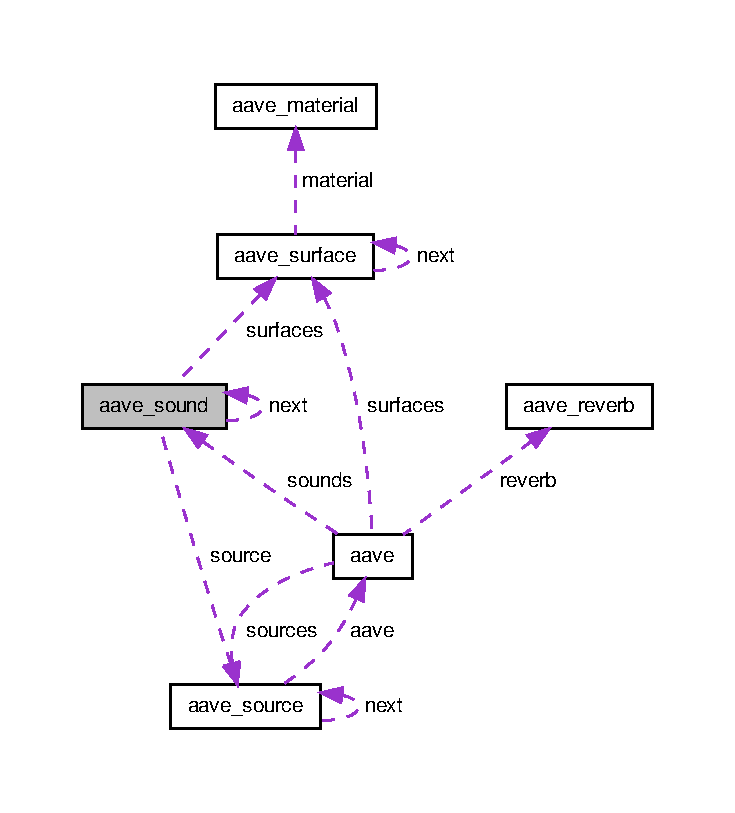
\includegraphics[width=350pt]{structaave__sound__coll__graph}
\end{center}
\end{figure}
\subsection*{Data Fields}
\begin{DoxyCompactItemize}
\item 
struct \hyperlink{structaave__sound}{aave\-\_\-sound} $\ast$ \hyperlink{structaave__sound_a3e64f8a8399ae64de4d5ebd266fd7eb3}{next}
\item 
struct \hyperlink{structaave__source}{aave\-\_\-source} $\ast$ \hyperlink{structaave__sound_ac56f4ab64afcb0668832301110e3bfdb}{source}
\item 
float $\ast$ \hyperlink{structaave__sound_a04a3c01ca0a54233061a2e2ebac1b464}{position}
\item 
int \hyperlink{structaave__sound_ad452524fd55cf2d6490a7a7b9a1c85b7}{audible}
\item 
unsigned \hyperlink{structaave__sound_ad4ce9aa0eca1519c53465d9704fd6efa}{fade\-\_\-samples}
\item 
float \hyperlink{structaave__sound_abefe2c52139bd0fcad1413d82ce1635e}{distance}
\item 
float \hyperlink{structaave__sound_a32919a754ba68db947c74eaadad979c2}{distance\-\_\-smooth}
\item 
const float $\ast$ \hyperlink{structaave__sound_a01efd817868c055126f2aea812a44d1a}{hrtf} \mbox{[}2\mbox{]}
\item 
struct \hyperlink{structaave__surface}{aave\-\_\-surface} $\ast$ \hyperlink{structaave__sound_a4d8cbff05fc5af52a18ac1c9015cfc97}{surfaces} \mbox{[}\hyperlink{aave_8h_a5cc7807cca10cf0933038ad388171181}{A\-A\-V\-E\-\_\-\-M\-A\-X\-\_\-\-R\-E\-F\-L\-E\-C\-T\-I\-O\-N\-S}\mbox{]}
\item 
float \hyperlink{structaave__sound_a0627e96d3a12a30fec75a65cc6f402a7}{image\-\_\-sources} \mbox{[}\hyperlink{aave_8h_a5cc7807cca10cf0933038ad388171181}{A\-A\-V\-E\-\_\-\-M\-A\-X\-\_\-\-R\-E\-F\-L\-E\-C\-T\-I\-O\-N\-S}\mbox{]}\mbox{[}3\mbox{]}
\item 
float \hyperlink{structaave__sound_a06b4b094d9e92084c8b10a99bfe74e5e}{reflection\-\_\-points} \mbox{[}\hyperlink{aave_8h_a5cc7807cca10cf0933038ad388171181}{A\-A\-V\-E\-\_\-\-M\-A\-X\-\_\-\-R\-E\-F\-L\-E\-C\-T\-I\-O\-N\-S}\mbox{]}\mbox{[}3\mbox{]}
\item 
float \hyperlink{structaave__sound_aa94c4070b91409c6cac4189fc599f6f9}{dft} \mbox{[}\hyperlink{aave_8h_a19ea3a18eb313fc3b825f522245d19d3}{A\-A\-V\-E\-\_\-\-M\-A\-X\-\_\-\-H\-R\-T\-F} $\ast$4\mbox{]}
\item 
float \hyperlink{structaave__sound_a6e27d4a259442303d940706031c2ee83}{filter} \mbox{[}\hyperlink{aave_8h_a19ea3a18eb313fc3b825f522245d19d3}{A\-A\-V\-E\-\_\-\-M\-A\-X\-\_\-\-H\-R\-T\-F} $\ast$4\mbox{]}
\end{DoxyCompactItemize}


\subsection{Detailed Description}
Data for each sound to auralise. 

\subsection{Field Documentation}
\hypertarget{structaave__sound_ad452524fd55cf2d6490a7a7b9a1c85b7}{\index{aave\-\_\-sound@{aave\-\_\-sound}!audible@{audible}}
\index{audible@{audible}!aave_sound@{aave\-\_\-sound}}
\subsubsection[{audible}]{\setlength{\rightskip}{0pt plus 5cm}int aave\-\_\-sound\-::audible}}\label{structaave__sound_ad452524fd55cf2d6490a7a7b9a1c85b7}
Flag that indicates if the sound is audible (1) or not (0). \hypertarget{structaave__sound_aa94c4070b91409c6cac4189fc599f6f9}{\index{aave\-\_\-sound@{aave\-\_\-sound}!dft@{dft}}
\index{dft@{dft}!aave_sound@{aave\-\_\-sound}}
\subsubsection[{dft}]{\setlength{\rightskip}{0pt plus 5cm}float aave\-\_\-sound\-::dft\mbox{[}{\bf A\-A\-V\-E\-\_\-\-M\-A\-X\-\_\-\-H\-R\-T\-F} $\ast$4\mbox{]}}}\label{structaave__sound_aa94c4070b91409c6cac4189fc599f6f9}
The D\-F\-T of the previous audio block. \hypertarget{structaave__sound_abefe2c52139bd0fcad1413d82ce1635e}{\index{aave\-\_\-sound@{aave\-\_\-sound}!distance@{distance}}
\index{distance@{distance}!aave_sound@{aave\-\_\-sound}}
\subsubsection[{distance}]{\setlength{\rightskip}{0pt plus 5cm}float aave\-\_\-sound\-::distance}}\label{structaave__sound_abefe2c52139bd0fcad1413d82ce1635e}
The previous distance value used (for the crossfading). \hypertarget{structaave__sound_a32919a754ba68db947c74eaadad979c2}{\index{aave\-\_\-sound@{aave\-\_\-sound}!distance\-\_\-smooth@{distance\-\_\-smooth}}
\index{distance\-\_\-smooth@{distance\-\_\-smooth}!aave_sound@{aave\-\_\-sound}}
\subsubsection[{distance\-\_\-smooth}]{\setlength{\rightskip}{0pt plus 5cm}float aave\-\_\-sound\-::distance\-\_\-smooth}}\label{structaave__sound_a32919a754ba68db947c74eaadad979c2}
Smooth (low-\/pass filtered) distance value (for the resampling). \hypertarget{structaave__sound_ad4ce9aa0eca1519c53465d9704fd6efa}{\index{aave\-\_\-sound@{aave\-\_\-sound}!fade\-\_\-samples@{fade\-\_\-samples}}
\index{fade\-\_\-samples@{fade\-\_\-samples}!aave_sound@{aave\-\_\-sound}}
\subsubsection[{fade\-\_\-samples}]{\setlength{\rightskip}{0pt plus 5cm}unsigned aave\-\_\-sound\-::fade\-\_\-samples}}\label{structaave__sound_ad4ce9aa0eca1519c53465d9704fd6efa}
The previous fade-\/in/out sample count value used (for the fade-\/in/out of appearing/disappearing sounds). \hypertarget{structaave__sound_a6e27d4a259442303d940706031c2ee83}{\index{aave\-\_\-sound@{aave\-\_\-sound}!filter@{filter}}
\index{filter@{filter}!aave_sound@{aave\-\_\-sound}}
\subsubsection[{filter}]{\setlength{\rightskip}{0pt plus 5cm}float aave\-\_\-sound\-::filter\mbox{[}{\bf A\-A\-V\-E\-\_\-\-M\-A\-X\-\_\-\-H\-R\-T\-F} $\ast$4\mbox{]}}}\label{structaave__sound_a6e27d4a259442303d940706031c2ee83}
The material absorption filter D\-F\-T. \hypertarget{structaave__sound_a01efd817868c055126f2aea812a44d1a}{\index{aave\-\_\-sound@{aave\-\_\-sound}!hrtf@{hrtf}}
\index{hrtf@{hrtf}!aave_sound@{aave\-\_\-sound}}
\subsubsection[{hrtf}]{\setlength{\rightskip}{0pt plus 5cm}const float$\ast$ aave\-\_\-sound\-::hrtf\mbox{[}2\mbox{]}}}\label{structaave__sound_a01efd817868c055126f2aea812a44d1a}
The previous H\-R\-T\-F pair used (for the crossfading). \hypertarget{structaave__sound_a0627e96d3a12a30fec75a65cc6f402a7}{\index{aave\-\_\-sound@{aave\-\_\-sound}!image\-\_\-sources@{image\-\_\-sources}}
\index{image\-\_\-sources@{image\-\_\-sources}!aave_sound@{aave\-\_\-sound}}
\subsubsection[{image\-\_\-sources}]{\setlength{\rightskip}{0pt plus 5cm}float aave\-\_\-sound\-::image\-\_\-sources\mbox{[}{\bf A\-A\-V\-E\-\_\-\-M\-A\-X\-\_\-\-R\-E\-F\-L\-E\-C\-T\-I\-O\-N\-S}\mbox{]}\mbox{[}3\mbox{]}}}\label{structaave__sound_a0627e96d3a12a30fec75a65cc6f402a7}
The image-\/source positions calculated for each reflection. \hypertarget{structaave__sound_a3e64f8a8399ae64de4d5ebd266fd7eb3}{\index{aave\-\_\-sound@{aave\-\_\-sound}!next@{next}}
\index{next@{next}!aave_sound@{aave\-\_\-sound}}
\subsubsection[{next}]{\setlength{\rightskip}{0pt plus 5cm}struct {\bf aave\-\_\-sound}$\ast$ aave\-\_\-sound\-::next}}\label{structaave__sound_a3e64f8a8399ae64de4d5ebd266fd7eb3}
Pointer to the next sound (singly-\/linked list). \hypertarget{structaave__sound_a04a3c01ca0a54233061a2e2ebac1b464}{\index{aave\-\_\-sound@{aave\-\_\-sound}!position@{position}}
\index{position@{position}!aave_sound@{aave\-\_\-sound}}
\subsubsection[{position}]{\setlength{\rightskip}{0pt plus 5cm}float$\ast$ aave\-\_\-sound\-::position}}\label{structaave__sound_a04a3c01ca0a54233061a2e2ebac1b464}
Position of the source or image-\/source of this sound \mbox{[}x,y,z\mbox{]} (m). If this is a direct sound, this points to source-\/$>$position. If it is a reflection, this points to image\-\_\-sources\mbox{[}order\mbox{]}. \hypertarget{structaave__sound_a06b4b094d9e92084c8b10a99bfe74e5e}{\index{aave\-\_\-sound@{aave\-\_\-sound}!reflection\-\_\-points@{reflection\-\_\-points}}
\index{reflection\-\_\-points@{reflection\-\_\-points}!aave_sound@{aave\-\_\-sound}}
\subsubsection[{reflection\-\_\-points}]{\setlength{\rightskip}{0pt plus 5cm}float aave\-\_\-sound\-::reflection\-\_\-points\mbox{[}{\bf A\-A\-V\-E\-\_\-\-M\-A\-X\-\_\-\-R\-E\-F\-L\-E\-C\-T\-I\-O\-N\-S}\mbox{]}\mbox{[}3\mbox{]}}}\label{structaave__sound_a06b4b094d9e92084c8b10a99bfe74e5e}
The points \mbox{[}x,y,z\mbox{]} where this sound reflects. \hypertarget{structaave__sound_ac56f4ab64afcb0668832301110e3bfdb}{\index{aave\-\_\-sound@{aave\-\_\-sound}!source@{source}}
\index{source@{source}!aave_sound@{aave\-\_\-sound}}
\subsubsection[{source}]{\setlength{\rightskip}{0pt plus 5cm}struct {\bf aave\-\_\-source}$\ast$ aave\-\_\-sound\-::source}}\label{structaave__sound_ac56f4ab64afcb0668832301110e3bfdb}
The sound source that is producing this sound. \hypertarget{structaave__sound_a4d8cbff05fc5af52a18ac1c9015cfc97}{\index{aave\-\_\-sound@{aave\-\_\-sound}!surfaces@{surfaces}}
\index{surfaces@{surfaces}!aave_sound@{aave\-\_\-sound}}
\subsubsection[{surfaces}]{\setlength{\rightskip}{0pt plus 5cm}struct {\bf aave\-\_\-surface}$\ast$ aave\-\_\-sound\-::surfaces\mbox{[}{\bf A\-A\-V\-E\-\_\-\-M\-A\-X\-\_\-\-R\-E\-F\-L\-E\-C\-T\-I\-O\-N\-S}\mbox{]}}}\label{structaave__sound_a4d8cbff05fc5af52a18ac1c9015cfc97}
The surfaces where this sound reflects. 

The documentation for this struct was generated from the following file\-:\begin{DoxyCompactItemize}
\item 
\hyperlink{aave_8h}{aave.\-h}\end{DoxyCompactItemize}

\hypertarget{structaave__source}{\section{aave\-\_\-source Struct Reference}
\label{structaave__source}\index{aave\-\_\-source@{aave\-\_\-source}}
}


{\ttfamily \#include $<$aave.\-h$>$}



Collaboration diagram for aave\-\_\-source\-:\nopagebreak
\begin{figure}[H]
\begin{center}
\leavevmode
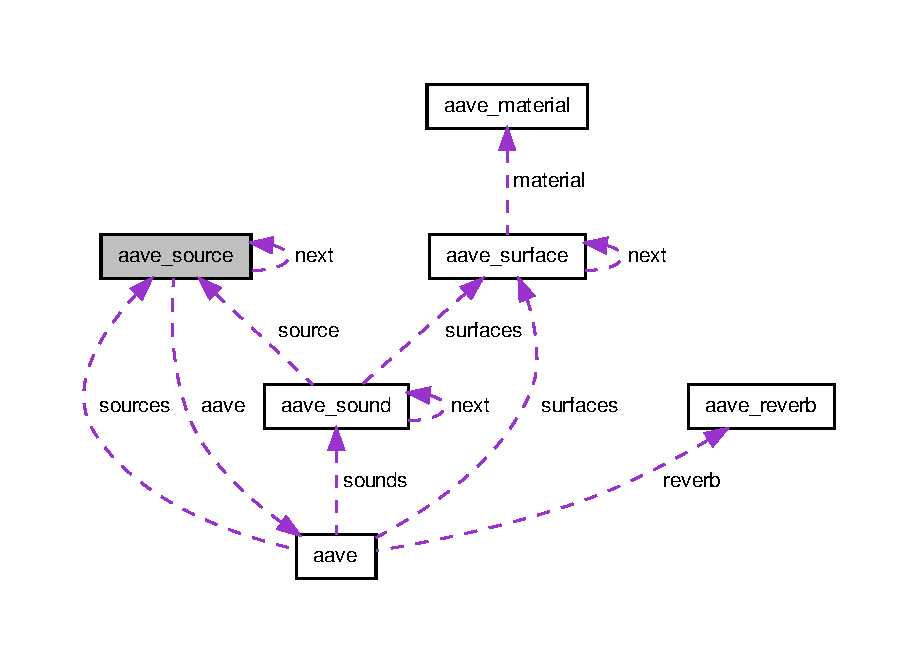
\includegraphics[width=350pt]{structaave__source__coll__graph}
\end{center}
\end{figure}
\subsection*{Data Fields}
\begin{DoxyCompactItemize}
\item 
struct \hyperlink{structaave__source}{aave\-\_\-source} $\ast$ \hyperlink{structaave__source_a987a6e5c5f722296854d0d1699fd53fa}{next}
\item 
struct \hyperlink{structaave}{aave} $\ast$ \hyperlink{structaave__source_a5c8d463d1960b8f5c9150f17e31ca230}{aave}
\item 
float \hyperlink{structaave__source_a1c5c2c95f27b846dac60d97cd3d6104e}{position} \mbox{[}3\mbox{]}
\item 
unsigned \hyperlink{structaave__source_a78b8739c3487c7f4cae4529e61063d64}{buffer\-\_\-index}
\item 
short \hyperlink{structaave__source_a25b0c8024c657431c670e52128c429fc}{buffer} \mbox{[}\hyperlink{aave_8h_a0b7b591faf4644c56f374fef7a6141bc}{A\-A\-V\-E\-\_\-\-S\-O\-U\-R\-C\-E\-\_\-\-B\-U\-F\-S\-I\-Z\-E}\mbox{]}
\end{DoxyCompactItemize}


\subsection{Detailed Description}
Data for each sound source in the auralisation world. \begin{Desc}
\item[Examples\-: ]\par
\hyperlink{examples_2circle_8c-example}{examples/circle.\-c}, \hyperlink{examples_2elevation_8c-example}{examples/elevation.\-c}, \hyperlink{examples_2line_8c-example}{examples/line.\-c}, and \hyperlink{examples_2stream_8c-example}{examples/stream.\-c}.\end{Desc}


\subsection{Field Documentation}
\hypertarget{structaave__source_a5c8d463d1960b8f5c9150f17e31ca230}{\index{aave\-\_\-source@{aave\-\_\-source}!aave@{aave}}
\index{aave@{aave}!aave_source@{aave\-\_\-source}}
\subsubsection[{aave}]{\setlength{\rightskip}{0pt plus 5cm}struct {\bf aave}$\ast$ aave\-\_\-source\-::aave}}\label{structaave__source_a5c8d463d1960b8f5c9150f17e31ca230}
The Acoustic\-A\-V\-E engine this sound source is associated with. \hypertarget{structaave__source_a25b0c8024c657431c670e52128c429fc}{\index{aave\-\_\-source@{aave\-\_\-source}!buffer@{buffer}}
\index{buffer@{buffer}!aave_source@{aave\-\_\-source}}
\subsubsection[{buffer}]{\setlength{\rightskip}{0pt plus 5cm}short aave\-\_\-source\-::buffer\mbox{[}{\bf A\-A\-V\-E\-\_\-\-S\-O\-U\-R\-C\-E\-\_\-\-B\-U\-F\-S\-I\-Z\-E}\mbox{]}}}\label{structaave__source_a25b0c8024c657431c670e52128c429fc}
Ring buffer to store the recent past anechoic samples. \begin{Desc}
\item[Examples\-: ]\par
\hyperlink{examples_2stream_8c-example}{examples/stream.\-c}.\end{Desc}
\hypertarget{structaave__source_a78b8739c3487c7f4cae4529e61063d64}{\index{aave\-\_\-source@{aave\-\_\-source}!buffer\-\_\-index@{buffer\-\_\-index}}
\index{buffer\-\_\-index@{buffer\-\_\-index}!aave_source@{aave\-\_\-source}}
\subsubsection[{buffer\-\_\-index}]{\setlength{\rightskip}{0pt plus 5cm}unsigned aave\-\_\-source\-::buffer\-\_\-index}}\label{structaave__source_a78b8739c3487c7f4cae4529e61063d64}
Index of the most recently inserted sample. \hypertarget{structaave__source_a987a6e5c5f722296854d0d1699fd53fa}{\index{aave\-\_\-source@{aave\-\_\-source}!next@{next}}
\index{next@{next}!aave_source@{aave\-\_\-source}}
\subsubsection[{next}]{\setlength{\rightskip}{0pt plus 5cm}struct {\bf aave\-\_\-source}$\ast$ aave\-\_\-source\-::next}}\label{structaave__source_a987a6e5c5f722296854d0d1699fd53fa}
Pointer to the next source (singly-\/linked list). \hypertarget{structaave__source_a1c5c2c95f27b846dac60d97cd3d6104e}{\index{aave\-\_\-source@{aave\-\_\-source}!position@{position}}
\index{position@{position}!aave_source@{aave\-\_\-source}}
\subsubsection[{position}]{\setlength{\rightskip}{0pt plus 5cm}float aave\-\_\-source\-::position\mbox{[}3\mbox{]}}}\label{structaave__source_a1c5c2c95f27b846dac60d97cd3d6104e}
Position of the source in the auralisation world \mbox{[}x,y,z\mbox{]} (m). 

The documentation for this struct was generated from the following file\-:\begin{DoxyCompactItemize}
\item 
\hyperlink{aave_8h}{aave.\-h}\end{DoxyCompactItemize}

\hypertarget{structaave__surface}{\section{aave\-\_\-surface Struct Reference}
\label{structaave__surface}\index{aave\-\_\-surface@{aave\-\_\-surface}}
}


{\ttfamily \#include $<$aave.\-h$>$}



Collaboration diagram for aave\-\_\-surface\-:\nopagebreak
\begin{figure}[H]
\begin{center}
\leavevmode
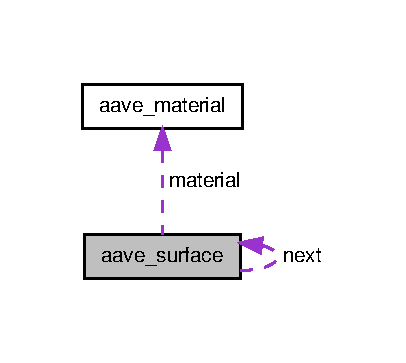
\includegraphics[width=195pt]{structaave__surface__coll__graph}
\end{center}
\end{figure}
\subsection*{Data Fields}
\begin{DoxyCompactItemize}
\item 
struct \hyperlink{structaave__surface}{aave\-\_\-surface} $\ast$ \hyperlink{structaave__surface_a4437c02a050c5cd3d99272bb3d5ebd7e}{next}
\item 
struct \hyperlink{structaave__material}{aave\-\_\-material} $\ast$ \hyperlink{structaave__surface_a6dfe11d4b9e97f9167a39669513a4b0a}{material}
\item 
float \hyperlink{structaave__surface_a9a12af46ca455c786a791ce484afdbd4}{avg\-\_\-absorption\-\_\-coef}
\item 
float \hyperlink{structaave__surface_a8b5aa68de342d90a056663c90fc31f28}{normal} \mbox{[}3\mbox{]}
\item 
\hypertarget{structaave__surface_a6a8499e479693fd5915cc070497b1701}{float {\bfseries distance}}\label{structaave__surface_a6a8499e479693fd5915cc070497b1701}

\item 
float \hyperlink{structaave__surface_a8724b22799063ed44d691a845f68f768}{versors} \mbox{[}2\mbox{]}\mbox{[}3\mbox{]}
\item 
unsigned \hyperlink{structaave__surface_a30f288c41c0a36c0a2492ab100e6c05c}{npoints}
\item 
float \hyperlink{structaave__surface_a6bd0e3127c052c7cf3ffa49480acda83}{points} \mbox{[}32\mbox{]}\mbox{[}3+2\mbox{]}
\end{DoxyCompactItemize}


\subsection{Detailed Description}
Data for each surface that makes the auralisation world. A surface is defined as an n-\/point planar polygon. The points are specified in anti-\/clockwise order. 

\subsection{Field Documentation}
\hypertarget{structaave__surface_a9a12af46ca455c786a791ce484afdbd4}{\index{aave\-\_\-surface@{aave\-\_\-surface}!avg\-\_\-absorption\-\_\-coef@{avg\-\_\-absorption\-\_\-coef}}
\index{avg\-\_\-absorption\-\_\-coef@{avg\-\_\-absorption\-\_\-coef}!aave_surface@{aave\-\_\-surface}}
\subsubsection[{avg\-\_\-absorption\-\_\-coef}]{\setlength{\rightskip}{0pt plus 5cm}float aave\-\_\-surface\-::avg\-\_\-absorption\-\_\-coef}}\label{structaave__surface_a9a12af46ca455c786a791ce484afdbd4}
Average absorption coeficient. \hypertarget{structaave__surface_a6dfe11d4b9e97f9167a39669513a4b0a}{\index{aave\-\_\-surface@{aave\-\_\-surface}!material@{material}}
\index{material@{material}!aave_surface@{aave\-\_\-surface}}
\subsubsection[{material}]{\setlength{\rightskip}{0pt plus 5cm}struct {\bf aave\-\_\-material}$\ast$ aave\-\_\-surface\-::material}}\label{structaave__surface_a6dfe11d4b9e97f9167a39669513a4b0a}
Material of the surface. \hypertarget{structaave__surface_a4437c02a050c5cd3d99272bb3d5ebd7e}{\index{aave\-\_\-surface@{aave\-\_\-surface}!next@{next}}
\index{next@{next}!aave_surface@{aave\-\_\-surface}}
\subsubsection[{next}]{\setlength{\rightskip}{0pt plus 5cm}struct {\bf aave\-\_\-surface}$\ast$ aave\-\_\-surface\-::next}}\label{structaave__surface_a4437c02a050c5cd3d99272bb3d5ebd7e}
Pointer to the next surface (singly-\/linked list). \hypertarget{structaave__surface_a8b5aa68de342d90a056663c90fc31f28}{\index{aave\-\_\-surface@{aave\-\_\-surface}!normal@{normal}}
\index{normal@{normal}!aave_surface@{aave\-\_\-surface}}
\subsubsection[{normal}]{\setlength{\rightskip}{0pt plus 5cm}float aave\-\_\-surface\-::normal\mbox{[}3\mbox{]}}}\label{structaave__surface_a8b5aa68de342d90a056663c90fc31f28}
Specification of the plane where this surface lays, in Hessian normal form\-: unit normal vector and distance from origin. (\href{http://mathworld.wolfram.com/HessianNormalForm.html}{\tt http\-://mathworld.\-wolfram.\-com/\-Hessian\-Normal\-Form.\-html}) The distance is used to calculate the position of the image sources. The unit normal vector is used just about everywhere. \hypertarget{structaave__surface_a30f288c41c0a36c0a2492ab100e6c05c}{\index{aave\-\_\-surface@{aave\-\_\-surface}!npoints@{npoints}}
\index{npoints@{npoints}!aave_surface@{aave\-\_\-surface}}
\subsubsection[{npoints}]{\setlength{\rightskip}{0pt plus 5cm}unsigned aave\-\_\-surface\-::npoints}}\label{structaave__surface_a30f288c41c0a36c0a2492ab100e6c05c}
Number of points of the polygon (minimum 3). \hypertarget{structaave__surface_a6bd0e3127c052c7cf3ffa49480acda83}{\index{aave\-\_\-surface@{aave\-\_\-surface}!points@{points}}
\index{points@{points}!aave_surface@{aave\-\_\-surface}}
\subsubsection[{points}]{\setlength{\rightskip}{0pt plus 5cm}float aave\-\_\-surface\-::points\mbox{[}32\mbox{]}\mbox{[}3+2\mbox{]}}}\label{structaave__surface_a6bd0e3127c052c7cf3ffa49480acda83}
Coordinates of each point, in counter-\/clockwise order (counter-\/clockwise normal).

World coordinates\-:
\begin{DoxyItemize}
\item x = points\mbox{[}i\mbox{]}\mbox{[}0\mbox{]}
\item y = points\mbox{[}i\mbox{]}\mbox{[}1\mbox{]}
\item z = points\mbox{[}i\mbox{]}\mbox{[}2\mbox{]}
\end{DoxyItemize}

Local coordinates (internally used by the polygon-\/line intersection algorithm)\-:
\begin{DoxyItemize}
\item ex = points\mbox{[}i\mbox{]}\mbox{[}3\mbox{]}
\item ex = points\mbox{[}i\mbox{]}\mbox{[}4\mbox{]}
\end{DoxyItemize}

\begin{DoxyRefDesc}{Todo}
\item[\hyperlink{todo__todo000004}{Todo}]Remove hardcoded maximum number of points per surface. \end{DoxyRefDesc}
\hypertarget{structaave__surface_a8724b22799063ed44d691a845f68f768}{\index{aave\-\_\-surface@{aave\-\_\-surface}!versors@{versors}}
\index{versors@{versors}!aave_surface@{aave\-\_\-surface}}
\subsubsection[{versors}]{\setlength{\rightskip}{0pt plus 5cm}float aave\-\_\-surface\-::versors\mbox{[}2\mbox{]}\mbox{[}3\mbox{]}}}\label{structaave__surface_a8724b22799063ed44d691a845f68f768}
Alternate specification of the plane where this surface lays using 2 versors and a point (points\mbox{[}0\mbox{]}). This is used to perform calculations in local coordinates, namely the non-\/convex polygon -\/ line intersection algorithm. 

The documentation for this struct was generated from the following file\-:\begin{DoxyCompactItemize}
\item 
\hyperlink{aave_8h}{aave.\-h}\end{DoxyCompactItemize}

\hypertarget{structabsorption__filter}{\section{absorption\-\_\-filter Struct Reference}
\label{structabsorption__filter}\index{absorption\-\_\-filter@{absorption\-\_\-filter}}
}
\subsection*{Data Fields}
\begin{DoxyCompactItemize}
\item 
float \hyperlink{structabsorption__filter_a3e56f97968252e954f08b92e2f5efcde}{y}
\end{DoxyCompactItemize}


\subsection{Detailed Description}
Data of a low-\/pass filter for frequency-\/dependent reverberation time. 

\subsection{Field Documentation}
\hypertarget{structabsorption__filter_a3e56f97968252e954f08b92e2f5efcde}{\index{absorption\-\_\-filter@{absorption\-\_\-filter}!y@{y}}
\index{y@{y}!absorption_filter@{absorption\-\_\-filter}}
\subsubsection[{y}]{\setlength{\rightskip}{0pt plus 5cm}float absorption\-\_\-filter\-::y}}\label{structabsorption__filter_a3e56f97968252e954f08b92e2f5efcde}
Previous output of the filter (y\mbox{[}n-\/1\mbox{]}). 

The documentation for this struct was generated from the following file\-:\begin{DoxyCompactItemize}
\item 
\hyperlink{reverb__jot_8c}{reverb\-\_\-jot.\-c}\end{DoxyCompactItemize}

\hypertarget{structallpass}{\section{allpass Struct Reference}
\label{structallpass}\index{allpass@{allpass}}
}
\subsection*{Data Fields}
\begin{DoxyCompactItemize}
\item 
float \hyperlink{structallpass_a386c2fb3676a8b9eb006427d14df5589}{tap}
\item 
unsigned \hyperlink{structallpass_a03c8893e240b738a3881026d1433930e}{index}
\item 
float \hyperlink{structallpass_a9a88e7125eb10d734a1a408c26cebe49}{buffer} \mbox{[}2656\mbox{]}
\end{DoxyCompactItemize}


\subsection{Detailed Description}
Data of an all-\/pass filter. 

\subsection{Field Documentation}
\hypertarget{structallpass_a9a88e7125eb10d734a1a408c26cebe49}{\index{allpass@{allpass}!buffer@{buffer}}
\index{buffer@{buffer}!allpass@{allpass}}
\subsubsection[{buffer}]{\setlength{\rightskip}{0pt plus 5cm}float allpass\-::buffer\mbox{[}2656\mbox{]}}}\label{structallpass_a9a88e7125eb10d734a1a408c26cebe49}
Buffer to store the inserted values. \begin{DoxyRefDesc}{Todo}
\item[\hyperlink{todo__todo000015}{Todo}]Set maximum delay from the delays of all all-\/pass blocks. \end{DoxyRefDesc}
\hypertarget{structallpass_a03c8893e240b738a3881026d1433930e}{\index{allpass@{allpass}!index@{index}}
\index{index@{index}!allpass@{allpass}}
\subsubsection[{index}]{\setlength{\rightskip}{0pt plus 5cm}unsigned allpass\-::index}}\label{structallpass_a03c8893e240b738a3881026d1433930e}
Index to the latest value inserted in the buffer. \hypertarget{structallpass_a386c2fb3676a8b9eb006427d14df5589}{\index{allpass@{allpass}!tap@{tap}}
\index{tap@{tap}!allpass@{allpass}}
\subsubsection[{tap}]{\setlength{\rightskip}{0pt plus 5cm}float allpass\-::tap}}\label{structallpass_a386c2fb3676a8b9eb006427d14df5589}
Value captured inside the feedback network. 

The documentation for this struct was generated from the following file\-:\begin{DoxyCompactItemize}
\item 
\hyperlink{reverb__dattorro_8c}{reverb\-\_\-dattorro.\-c}\end{DoxyCompactItemize}

\hypertarget{structdc__block__filter}{\section{dc\-\_\-block\-\_\-filter Struct Reference}
\label{structdc__block__filter}\index{dc\-\_\-block\-\_\-filter@{dc\-\_\-block\-\_\-filter}}
}
\subsection*{Data Fields}
\begin{DoxyCompactItemize}
\item 
float \hyperlink{structdc__block__filter_ac47f2dcae35a1948fb7280f8b9fb34cd}{y}
\item 
float \hyperlink{structdc__block__filter_a51740a56346e009262b43b57937412af}{x}
\item 
float \hyperlink{structdc__block__filter_a368d9cdea5bf60962e415f9958d0c296}{b}
\end{DoxyCompactItemize}


\subsection{Detailed Description}
Data of a dc block filter for a rough reverb highpass. \begin{DoxyRefDesc}{Todo}
\item[\hyperlink{todo__todo000017}{Todo}]Improve bandwidth definition. \end{DoxyRefDesc}


\subsection{Field Documentation}
\hypertarget{structdc__block__filter_a368d9cdea5bf60962e415f9958d0c296}{\index{dc\-\_\-block\-\_\-filter@{dc\-\_\-block\-\_\-filter}!b@{b}}
\index{b@{b}!dc_block_filter@{dc\-\_\-block\-\_\-filter}}
\subsubsection[{b}]{\setlength{\rightskip}{0pt plus 5cm}float dc\-\_\-block\-\_\-filter\-::b}}\label{structdc__block__filter_a368d9cdea5bf60962e415f9958d0c296}
bandwidth. \hypertarget{structdc__block__filter_a51740a56346e009262b43b57937412af}{\index{dc\-\_\-block\-\_\-filter@{dc\-\_\-block\-\_\-filter}!x@{x}}
\index{x@{x}!dc_block_filter@{dc\-\_\-block\-\_\-filter}}
\subsubsection[{x}]{\setlength{\rightskip}{0pt plus 5cm}float dc\-\_\-block\-\_\-filter\-::x}}\label{structdc__block__filter_a51740a56346e009262b43b57937412af}
Previous input of the filter (x\mbox{[}n-\/1\mbox{]}). \hypertarget{structdc__block__filter_ac47f2dcae35a1948fb7280f8b9fb34cd}{\index{dc\-\_\-block\-\_\-filter@{dc\-\_\-block\-\_\-filter}!y@{y}}
\index{y@{y}!dc_block_filter@{dc\-\_\-block\-\_\-filter}}
\subsubsection[{y}]{\setlength{\rightskip}{0pt plus 5cm}float dc\-\_\-block\-\_\-filter\-::y}}\label{structdc__block__filter_ac47f2dcae35a1948fb7280f8b9fb34cd}
Previous output of the filter (y\mbox{[}n-\/1\mbox{]}). 

The documentation for this struct was generated from the following file\-:\begin{DoxyCompactItemize}
\item 
\hyperlink{reverb__jot_8c}{reverb\-\_\-jot.\-c}\end{DoxyCompactItemize}

\hypertarget{structdecay__block}{\section{decay\-\_\-block Struct Reference}
\label{structdecay__block}\index{decay\-\_\-block@{decay\-\_\-block}}
}


Collaboration diagram for decay\-\_\-block\-:\nopagebreak
\begin{figure}[H]
\begin{center}
\leavevmode
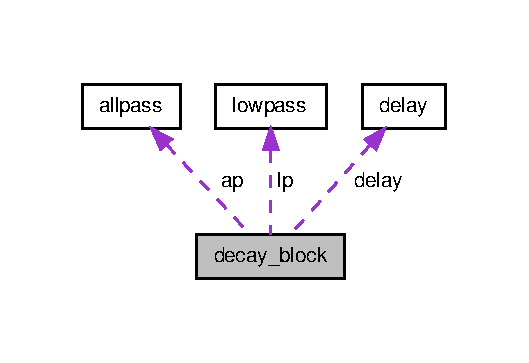
\includegraphics[width=254pt]{structdecay__block__coll__graph}
\end{center}
\end{figure}
\subsection*{Data Fields}
\begin{DoxyCompactItemize}
\item 
float \hyperlink{structdecay__block_ab25f987c34d1ec2d9cf019fc758bc196}{out}
\item 
struct \hyperlink{structlowpass}{lowpass} \hyperlink{structdecay__block_abe3a5f9a9c4bbb4873364861dfd2e1c6}{lp}
\item 
struct \hyperlink{structallpass}{allpass} \hyperlink{structdecay__block_a3f47e2dbc49bfba0a48954341342fea5}{ap} \mbox{[}2\mbox{]}
\item 
struct \hyperlink{structdelay}{delay} \hyperlink{structdecay__block_a954ff93051d7dfe61d76f24270618dc8}{delay} \mbox{[}2\mbox{]}
\end{DoxyCompactItemize}


\subsection{Detailed Description}
Data of a decay block. 

\subsection{Field Documentation}
\hypertarget{structdecay__block_a3f47e2dbc49bfba0a48954341342fea5}{\index{decay\-\_\-block@{decay\-\_\-block}!ap@{ap}}
\index{ap@{ap}!decay_block@{decay\-\_\-block}}
\subsubsection[{ap}]{\setlength{\rightskip}{0pt plus 5cm}struct {\bf allpass} decay\-\_\-block\-::ap\mbox{[}2\mbox{]}}}\label{structdecay__block_a3f47e2dbc49bfba0a48954341342fea5}
The decay all-\/pass filters. \hypertarget{structdecay__block_a954ff93051d7dfe61d76f24270618dc8}{\index{decay\-\_\-block@{decay\-\_\-block}!delay@{delay}}
\index{delay@{delay}!decay_block@{decay\-\_\-block}}
\subsubsection[{delay}]{\setlength{\rightskip}{0pt plus 5cm}struct {\bf delay} decay\-\_\-block\-::delay\mbox{[}2\mbox{]}}}\label{structdecay__block_a954ff93051d7dfe61d76f24270618dc8}
The delay lines. \hypertarget{structdecay__block_abe3a5f9a9c4bbb4873364861dfd2e1c6}{\index{decay\-\_\-block@{decay\-\_\-block}!lp@{lp}}
\index{lp@{lp}!decay_block@{decay\-\_\-block}}
\subsubsection[{lp}]{\setlength{\rightskip}{0pt plus 5cm}struct {\bf lowpass} decay\-\_\-block\-::lp}}\label{structdecay__block_abe3a5f9a9c4bbb4873364861dfd2e1c6}
The dampping low-\/pass filter. \hypertarget{structdecay__block_ab25f987c34d1ec2d9cf019fc758bc196}{\index{decay\-\_\-block@{decay\-\_\-block}!out@{out}}
\index{out@{out}!decay_block@{decay\-\_\-block}}
\subsubsection[{out}]{\setlength{\rightskip}{0pt plus 5cm}float decay\-\_\-block\-::out}}\label{structdecay__block_ab25f987c34d1ec2d9cf019fc758bc196}
The previous output value. 

The documentation for this struct was generated from the following file\-:\begin{DoxyCompactItemize}
\item 
\hyperlink{reverb__dattorro_8c}{reverb\-\_\-dattorro.\-c}\end{DoxyCompactItemize}

\hypertarget{structdelay}{\section{delay Struct Reference}
\label{structdelay}\index{delay@{delay}}
}
\subsection*{Data Fields}
\begin{DoxyCompactItemize}
\item 
unsigned \hyperlink{structdelay_ad94bb0da4af737feaa3e6136199fb7d6}{index}
\item 
float \hyperlink{structdelay_a655d8b9f8d1bcd90764042b7e6e58ea7}{buffer} \mbox{[}16384\mbox{]}
\end{DoxyCompactItemize}


\subsection{Detailed Description}
Data of a delay block. 

\subsection{Field Documentation}
\hypertarget{structdelay_a655d8b9f8d1bcd90764042b7e6e58ea7}{\index{delay@{delay}!buffer@{buffer}}
\index{buffer@{buffer}!delay@{delay}}
\subsubsection[{buffer}]{\setlength{\rightskip}{0pt plus 5cm}float delay\-::buffer\mbox{[}16384\mbox{]}}}\label{structdelay_a655d8b9f8d1bcd90764042b7e6e58ea7}
Buffer to store the inserted values. \begin{DoxyRefDesc}{Todo}
\item[\hyperlink{todo__todo000014}{Todo}]Set maximum delay from the delays of all delay blocks. \end{DoxyRefDesc}
\hypertarget{structdelay_ad94bb0da4af737feaa3e6136199fb7d6}{\index{delay@{delay}!index@{index}}
\index{index@{index}!delay@{delay}}
\subsubsection[{index}]{\setlength{\rightskip}{0pt plus 5cm}unsigned delay\-::index}}\label{structdelay_ad94bb0da4af737feaa3e6136199fb7d6}
Index to the latest value inserted in the buffer. 

The documentation for this struct was generated from the following file\-:\begin{DoxyCompactItemize}
\item 
\hyperlink{reverb__dattorro_8c}{reverb\-\_\-dattorro.\-c}\end{DoxyCompactItemize}

\hypertarget{structdelay__filter}{\section{delay\-\_\-filter Struct Reference}
\label{structdelay__filter}\index{delay\-\_\-filter@{delay\-\_\-filter}}
}
\subsection*{Data Fields}
\begin{DoxyCompactItemize}
\item 
unsigned \hyperlink{structdelay__filter_a7e5aab680dba8c144add99d4cd3dba3c}{index}
\item 
float \hyperlink{structdelay__filter_a7088bc142cec2c8cac8c47b60a9af09d}{buffer} \mbox{[}\hyperlink{reverb__jot_8c_a92d268dc3052f4e79fedd139859b0c8f}{M\-A\-X\-\_\-\-D\-E\-L\-A\-Y\-\_\-\-T\-I\-M\-E}\mbox{]}
\end{DoxyCompactItemize}


\subsection{Detailed Description}
Data of a delay filter. 

\subsection{Field Documentation}
\hypertarget{structdelay__filter_a7088bc142cec2c8cac8c47b60a9af09d}{\index{delay\-\_\-filter@{delay\-\_\-filter}!buffer@{buffer}}
\index{buffer@{buffer}!delay_filter@{delay\-\_\-filter}}
\subsubsection[{buffer}]{\setlength{\rightskip}{0pt plus 5cm}float delay\-\_\-filter\-::buffer\mbox{[}{\bf M\-A\-X\-\_\-\-D\-E\-L\-A\-Y\-\_\-\-T\-I\-M\-E}\mbox{]}}}\label{structdelay__filter_a7088bc142cec2c8cac8c47b60a9af09d}
Buffer to store the inserted values. \hypertarget{structdelay__filter_a7e5aab680dba8c144add99d4cd3dba3c}{\index{delay\-\_\-filter@{delay\-\_\-filter}!index@{index}}
\index{index@{index}!delay_filter@{delay\-\_\-filter}}
\subsubsection[{index}]{\setlength{\rightskip}{0pt plus 5cm}unsigned delay\-\_\-filter\-::index}}\label{structdelay__filter_a7e5aab680dba8c144add99d4cd3dba3c}
Index to the latest value inserted in the buffer. 

The documentation for this struct was generated from the following file\-:\begin{DoxyCompactItemize}
\item 
\hyperlink{reverb__jot_8c}{reverb\-\_\-jot.\-c}\end{DoxyCompactItemize}

\hypertarget{structlowpass}{\section{lowpass Struct Reference}
\label{structlowpass}\index{lowpass@{lowpass}}
}
\subsection*{Data Fields}
\begin{DoxyCompactItemize}
\item 
float \hyperlink{structlowpass_a3045b839fbd6e8f04f40a6bac79f8faa}{y}
\end{DoxyCompactItemize}


\subsection{Detailed Description}
Data of a low-\/pass filter. 

\subsection{Field Documentation}
\hypertarget{structlowpass_a3045b839fbd6e8f04f40a6bac79f8faa}{\index{lowpass@{lowpass}!y@{y}}
\index{y@{y}!lowpass@{lowpass}}
\subsubsection[{y}]{\setlength{\rightskip}{0pt plus 5cm}float lowpass\-::y}}\label{structlowpass_a3045b839fbd6e8f04f40a6bac79f8faa}
Previous output of the filter (y\mbox{[}n-\/1\mbox{]}). 

The documentation for this struct was generated from the following file\-:\begin{DoxyCompactItemize}
\item 
\hyperlink{reverb__dattorro_8c}{reverb\-\_\-dattorro.\-c}\end{DoxyCompactItemize}

\hypertarget{structtone__correction__filter}{\section{tone\-\_\-correction\-\_\-filter Struct Reference}
\label{structtone__correction__filter}\index{tone\-\_\-correction\-\_\-filter@{tone\-\_\-correction\-\_\-filter}}
}
\subsection*{Data Fields}
\begin{DoxyCompactItemize}
\item 
float \hyperlink{structtone__correction__filter_a33336212375a5062fd1b8d76a102c373}{y}
\end{DoxyCompactItemize}


\subsection{Detailed Description}
Data of a tone correction (high pass) filter. 

\subsection{Field Documentation}
\hypertarget{structtone__correction__filter_a33336212375a5062fd1b8d76a102c373}{\index{tone\-\_\-correction\-\_\-filter@{tone\-\_\-correction\-\_\-filter}!y@{y}}
\index{y@{y}!tone_correction_filter@{tone\-\_\-correction\-\_\-filter}}
\subsubsection[{y}]{\setlength{\rightskip}{0pt plus 5cm}float tone\-\_\-correction\-\_\-filter\-::y}}\label{structtone__correction__filter_a33336212375a5062fd1b8d76a102c373}
Previous output of the filter (y\mbox{[}n-\/1\mbox{]}). 

The documentation for this struct was generated from the following file\-:\begin{DoxyCompactItemize}
\item 
\hyperlink{reverb__jot_8c}{reverb\-\_\-jot.\-c}\end{DoxyCompactItemize}

\chapter{File Documentation}
\hypertarget{aave_8h}{\section{aave.\-h File Reference}
\label{aave_8h}\index{aave.\-h@{aave.\-h}}
}
This graph shows which files directly or indirectly include this file\-:\nopagebreak
\begin{figure}[H]
\begin{center}
\leavevmode
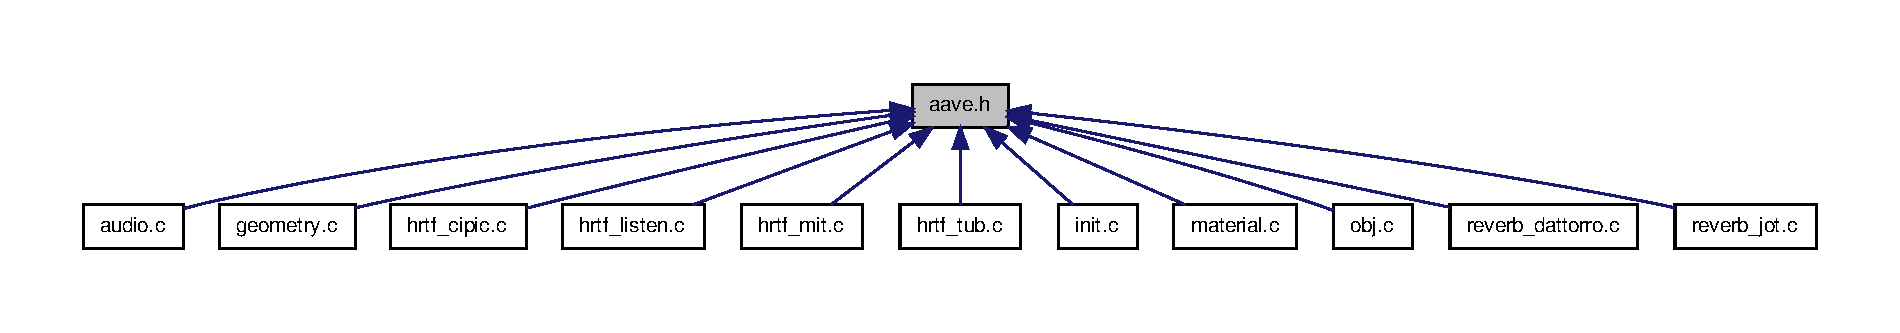
\includegraphics[width=350pt]{aave_8h__dep__incl}
\end{center}
\end{figure}
\subsection*{Data Structures}
\begin{DoxyCompactItemize}
\item 
struct \hyperlink{structaave}{aave}
\item 
struct \hyperlink{structaave__source}{aave\-\_\-source}
\item 
struct \hyperlink{structaave__surface}{aave\-\_\-surface}
\item 
struct \hyperlink{structaave__sound}{aave\-\_\-sound}
\item 
struct \hyperlink{structaave__material}{aave\-\_\-material}
\item 
struct \hyperlink{structaave__reverb}{aave\-\_\-reverb}
\end{DoxyCompactItemize}
\subsection*{Macros}
\begin{DoxyCompactItemize}
\item 
\#define \hyperlink{aave_8h_aff6fdc3178c7698a824bf53f79d0bdd1}{A\-A\-V\-E\-\_\-\-F\-S}~44100
\item 
\#define \hyperlink{aave_8h_a5cc7807cca10cf0933038ad388171181}{A\-A\-V\-E\-\_\-\-M\-A\-X\-\_\-\-R\-E\-F\-L\-E\-C\-T\-I\-O\-N\-S}~16
\item 
\#define \hyperlink{aave_8h_a19ea3a18eb313fc3b825f522245d19d3}{A\-A\-V\-E\-\_\-\-M\-A\-X\-\_\-\-H\-R\-T\-F}~2048
\item 
\#define \hyperlink{aave_8h_a0b7b591faf4644c56f374fef7a6141bc}{A\-A\-V\-E\-\_\-\-S\-O\-U\-R\-C\-E\-\_\-\-B\-U\-F\-S\-I\-Z\-E}~131072
\item 
\#define \hyperlink{aave_8h_ad76f6ee2a275c27185c10ff7ea5187b2}{A\-A\-V\-E\-\_\-\-M\-A\-T\-E\-R\-I\-A\-L\-\_\-\-R\-E\-F\-L\-E\-C\-T\-I\-O\-N\-\_\-\-F\-A\-C\-T\-O\-R\-S}~7
\item 
\#define \hyperlink{aave_8h_a94b17b055640b1a1593d032048ba3ed2}{A\-A\-V\-E\-\_\-\-S\-O\-U\-N\-D\-\_\-\-S\-P\-E\-E\-D}~343.\-2
\item 
\#define \hyperlink{aave_8h_aa8ac0978ba9be33dd450abaaa2dda4d9}{F\-D\-N\-\_\-\-O\-R\-D\-E\-R}~64
\end{DoxyCompactItemize}
\subsection*{Functions}
\begin{DoxyCompactItemize}
\item 
void \hyperlink{aave_8h_a8a63aae9a55200e05235e6e89990f1c6}{aave\-\_\-get\-\_\-audio} (struct \hyperlink{structaave}{aave} $\ast$, short $\ast$, unsigned)
\item 
void \hyperlink{aave_8h_a546bf3fff8b9009ddc744a6908154f5e}{aave\-\_\-put\-\_\-audio} (struct \hyperlink{structaave__source}{aave\-\_\-source} $\ast$, const short $\ast$, unsigned)
\item 
unsigned \hyperlink{aave_8h_a5b453c8df5597105b3a7cde336e83e0e}{dft\-\_\-index} (unsigned, unsigned)
\item 
void \hyperlink{aave_8h_af609d22b339f6a53d988e4c73f4b7dfb}{aave\-\_\-add\-\_\-source} (struct \hyperlink{structaave}{aave} $\ast$, struct \hyperlink{structaave__source}{aave\-\_\-source} $\ast$)
\item 
void \hyperlink{aave_8h_a20e98109bd38d422444f2959c0a6b80c}{aave\-\_\-add\-\_\-surface} (struct \hyperlink{structaave}{aave} $\ast$, struct \hyperlink{structaave__surface}{aave\-\_\-surface} $\ast$)
\item 
void \hyperlink{aave_8h_a98cd836fde1ac54fc6dcbb3aab416d8b}{aave\-\_\-get\-\_\-coordinates} (const struct \hyperlink{structaave}{aave} $\ast$, const float $\ast$, float $\ast$, float $\ast$, float $\ast$)
\item 
void \hyperlink{aave_8h_aee300969973298dab868f91f7b94724d}{aave\-\_\-set\-\_\-listener\-\_\-orientation} (struct \hyperlink{structaave}{aave} $\ast$, float, float, float)
\item 
void \hyperlink{aave_8h_a41a4224263cd8432d79099871d542b2e}{aave\-\_\-set\-\_\-listener\-\_\-position} (struct \hyperlink{structaave}{aave} $\ast$, float, float, float)
\item 
void \hyperlink{aave_8h_ad48ffc19be78794acb7bf0f9a6397c11}{aave\-\_\-set\-\_\-source\-\_\-position} (struct \hyperlink{structaave__source}{aave\-\_\-source} $\ast$, float, float, float)
\item 
void \hyperlink{aave_8h_a5acfa7c6e7e714ff364cda9dabd7a2f8}{aave\-\_\-update} (struct \hyperlink{structaave}{aave} $\ast$)
\item 
void \hyperlink{aave_8h_a9332f29f538c0e54272f61de0e420348}{aave\-\_\-hrtf\-\_\-cipic} (struct \hyperlink{structaave}{aave} $\ast$)
\item 
void \hyperlink{aave_8h_a1714770c36978ec1bfc9b4b5148e42be}{aave\-\_\-hrtf\-\_\-listen} (struct \hyperlink{structaave}{aave} $\ast$)
\item 
void \hyperlink{aave_8h_aad4aa8bf733bedef0ee981bbeffc1b12}{aave\-\_\-hrtf\-\_\-mit} (struct \hyperlink{structaave}{aave} $\ast$)
\item 
void \hyperlink{aave_8h_afbc85e87d1aaab2c91c7f15d1d5a9906}{aave\-\_\-hrtf\-\_\-tub} (struct \hyperlink{structaave}{aave} $\ast$)
\item 
void \hyperlink{aave_8h_a044e13c0826108a728f0b6324c23fbab}{aave\-\_\-init} (struct \hyperlink{structaave}{aave} $\ast$, unsigned)
\item 
void \hyperlink{aave_8h_a3682cd98f3556ad2b8c8e0bc8502371c}{aave\-\_\-init\-\_\-source} (struct \hyperlink{structaave}{aave} $\ast$, struct \hyperlink{structaave__source}{aave\-\_\-source} $\ast$)
\item 
struct \hyperlink{structaave__material}{aave\-\_\-material} $\ast$ \hyperlink{aave_8h_a952abc42265cb150fa647c008e8ee937}{aave\-\_\-get\-\_\-material} (const char $\ast$)
\item 
void \hyperlink{aave_8h_a300799824871774e895676f347905cf3}{aave\-\_\-get\-\_\-material\-\_\-filter} (struct \hyperlink{structaave}{aave} $\ast$, struct \hyperlink{structaave__surface}{aave\-\_\-surface} $\ast$$\ast$, unsigned, float $\ast$)
\item 
void \hyperlink{aave_8h_a7e664852f336438524336bdcac8be8bc}{aave\-\_\-read\-\_\-obj} (struct \hyperlink{structaave}{aave} $\ast$, const char $\ast$, unsigned, unsigned)
\item 
void \hyperlink{aave_8h_a87108aa6128bb303f58c46307a4b4ebb}{aave\-\_\-reverb\-\_\-dattorro} (struct \hyperlink{structaave}{aave} $\ast$, short $\ast$, unsigned)
\item 
void \hyperlink{aave_8h_aa5850eee4b27f5b7f2732f3457e00d79}{aave\-\_\-reverb\-\_\-jot} (struct \hyperlink{structaave}{aave} $\ast$, short $\ast$, unsigned)
\item 
void \hyperlink{aave_8h_a08e9496e914691f6f87708b74992020e}{init\-\_\-reverb} (struct \hyperlink{structaave__reverb}{aave\-\_\-reverb} $\ast$, float, float, float)
\item 
\hypertarget{aave_8h_a4b8e2ff48d88c6d2cbb9959f7d870d7c}{void {\bfseries print\-\_\-reverb\-\_\-parameters} (struct \hyperlink{structaave}{aave} $\ast$, struct \hyperlink{structaave__reverb}{aave\-\_\-reverb} $\ast$)}\label{aave_8h_a4b8e2ff48d88c6d2cbb9959f7d870d7c}

\end{DoxyCompactItemize}
\subsection*{Variables}
\begin{DoxyCompactItemize}
\item 
struct \hyperlink{structaave__material}{aave\-\_\-material} \hyperlink{aave_8h_a49ce2ac99af8e6a499e6b6dfa8962e58}{aave\-\_\-material\-\_\-none}
\end{DoxyCompactItemize}


\subsection{Detailed Description}
The \hyperlink{aave_8h}{aave.\-h} file is the public header file of the Acoustic\-A\-A\-V\-E library (libaave). It contains the declarations of the structures and functions used and implemented by the library. Include it from your program source files to use them.

The following diagram provides an overview of the data structures in the library and their associations.


\begin{DoxyImage}
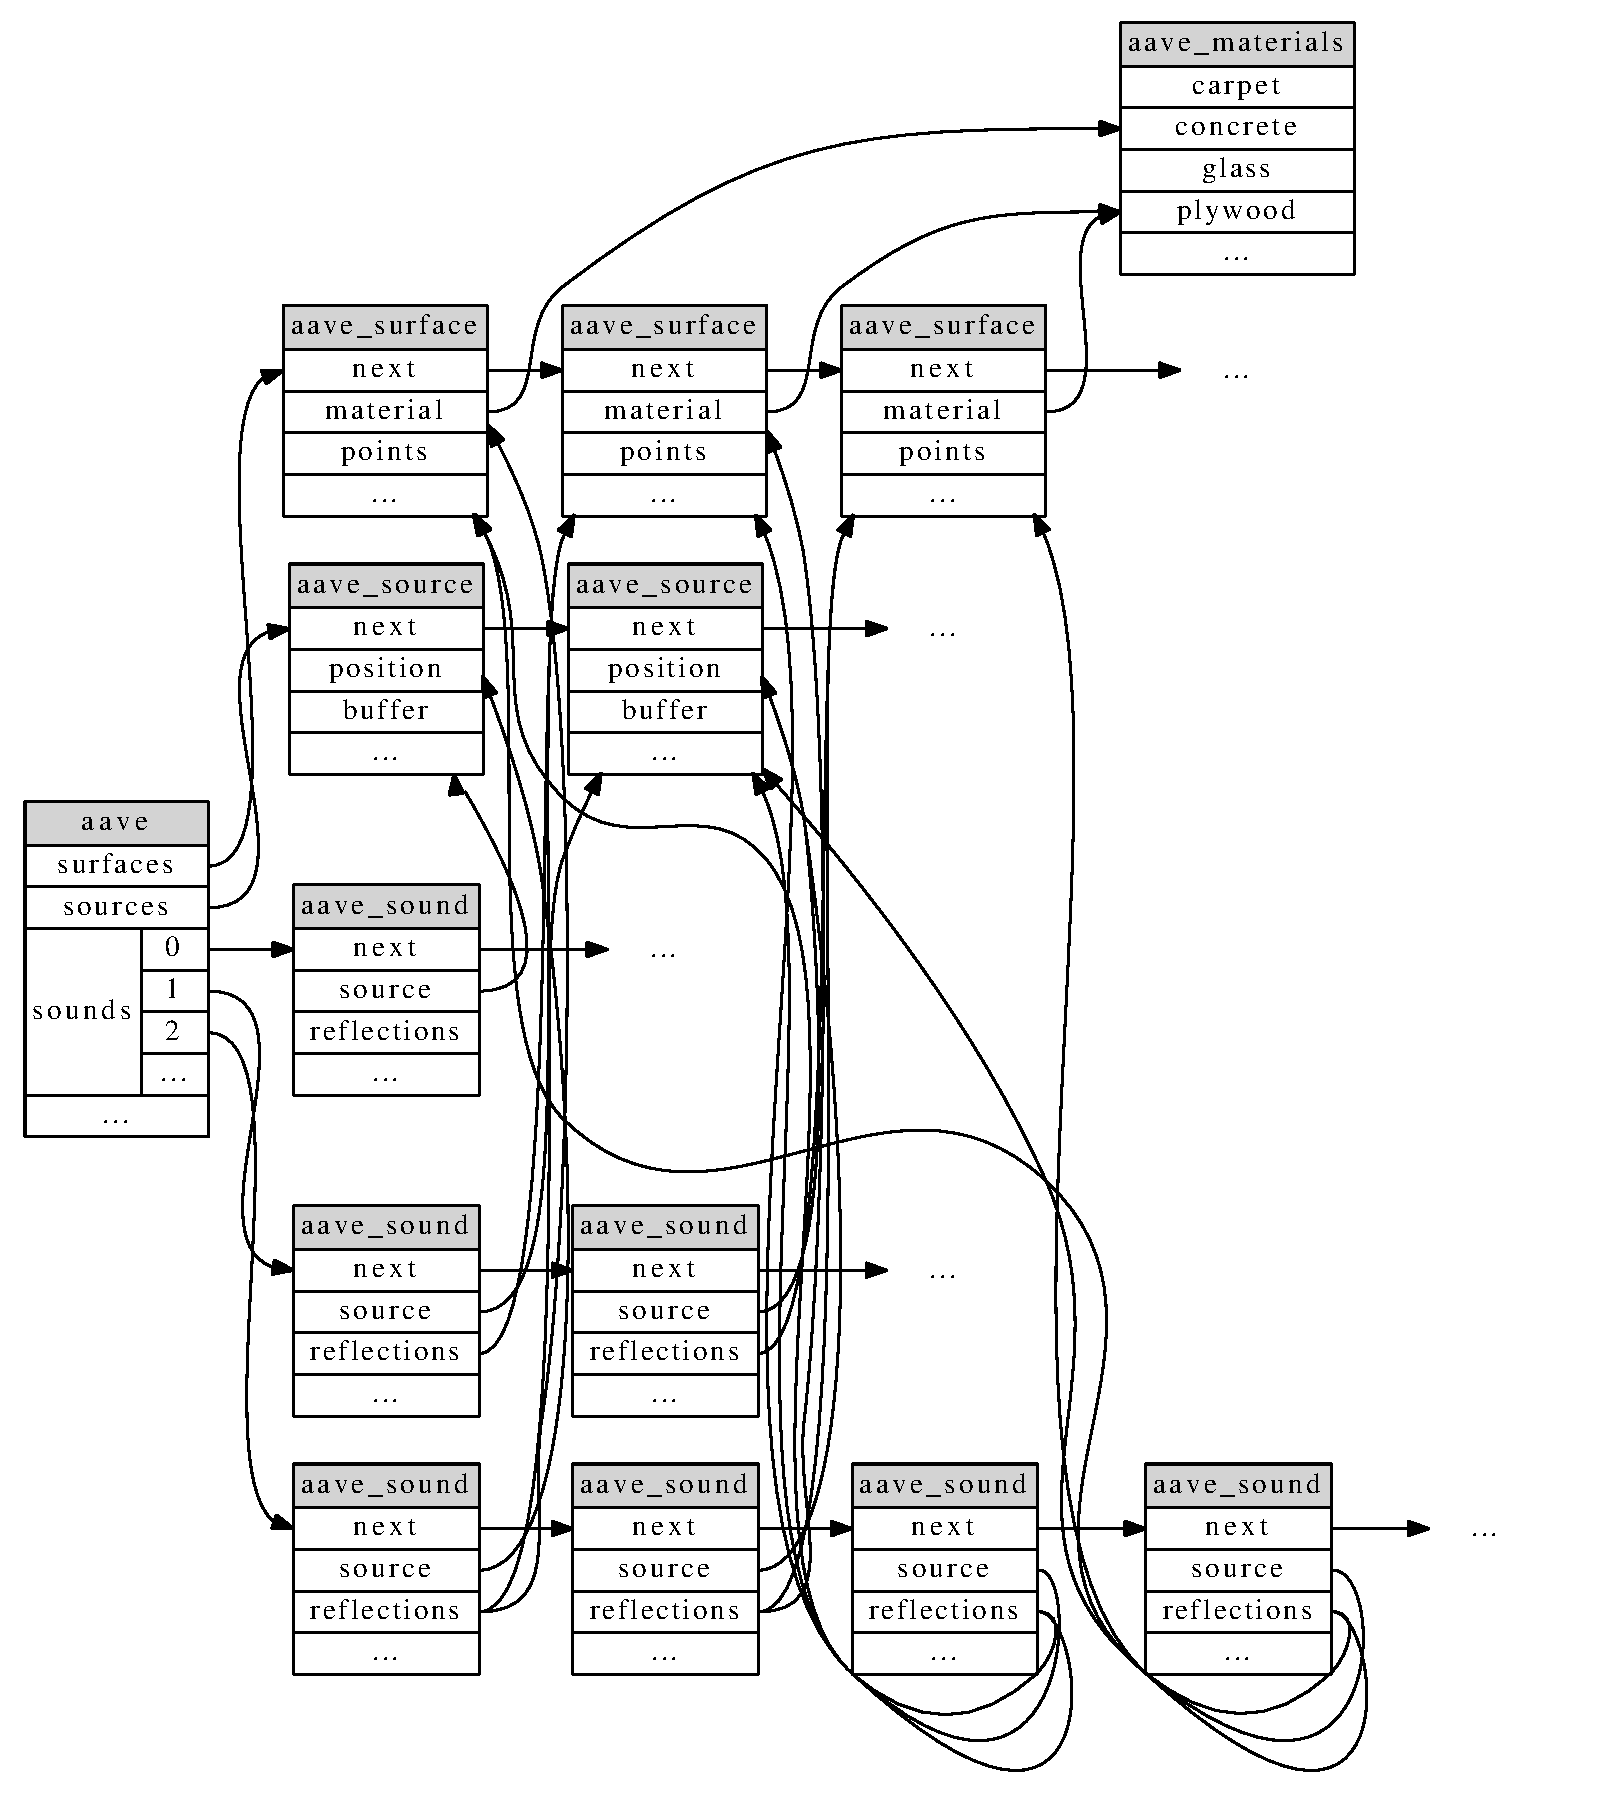
\includegraphics[width=\textwidth]{aave}
\caption{Data structure diagram}
\end{DoxyImage}


The aave structure is the main data structure of the Acoustic\-A\-V\-E library. It contains all necessary information to completely define an auralisation world and its present auralisation state.

The aave structure contains a list of \hyperlink{structaave__surface}{aave\-\_\-surface} structures. These surfaces define the geometry of the auralisation world. The material of each surface is indicated by pointing to the corresponding element in the aave\-\_\-materials table.

The aave structure contains a list of \hyperlink{structaave__source}{aave\-\_\-source} structures, one for each sound source present in the auralisation world.

The sound sources and surfaces in the auralisation world generate a number of sounds that reach the listener, and that are to be auralised by the library. These sounds are stored in the aave structure in a hash table indexed by the reflection order\-: direct sounds are put in the list of \hyperlink{structaave__sound}{aave\-\_\-sound} structures pointed by sounds\mbox{[}0\mbox{]}, 1st reflection sounds are put in sounds\mbox{[}1\mbox{]}, 2nd reflections in sounds\mbox{[}2\mbox{]}, etc... The \hyperlink{aave_8h_a5acfa7c6e7e714ff364cda9dabd7a2f8}{aave\-\_\-update()} function is responsible for maintaining the hash table up to date, and the \hyperlink{aave_8h_a8a63aae9a55200e05235e6e89990f1c6}{aave\-\_\-get\-\_\-audio()} function is responsible for auralising all sounds currently in it.

Each \hyperlink{structaave__sound}{aave\-\_\-sound} structure contains a reference to its sound source and references to each surface where that sound reflects. 

\subsection{Macro Definition Documentation}
\hypertarget{aave_8h_aff6fdc3178c7698a824bf53f79d0bdd1}{\index{aave.\-h@{aave.\-h}!A\-A\-V\-E\-\_\-\-F\-S@{A\-A\-V\-E\-\_\-\-F\-S}}
\index{A\-A\-V\-E\-\_\-\-F\-S@{A\-A\-V\-E\-\_\-\-F\-S}!aave.h@{aave.\-h}}
\subsubsection[{A\-A\-V\-E\-\_\-\-F\-S}]{\setlength{\rightskip}{0pt plus 5cm}\#define A\-A\-V\-E\-\_\-\-F\-S~44100}}\label{aave_8h_aff6fdc3178c7698a824bf53f79d0bdd1}
The audio sampling frequency, in Hz, used throughout the library. In particular, libaave expects the anechoic input data of the sound sources to be delivered in this sampling frequency. The auralisation binaural output data is also in this sampling frequency.

\begin{DoxyRefDesc}{Todo}
\item[\hyperlink{todo__todo000001}{Todo}]To support different audio sampling frequencies without having to recompile the library, this value would be set in a member of the aave structure at runtime instead. Of course, that would incur in performance penalties, most importantly in the audio processing (one floating-\/point division per audio sample per auralised sound). Furthermore, the H\-R\-T\-F data sets would have to be resampled to the desired sampling frequency. \end{DoxyRefDesc}
\begin{Desc}
\item[Examples\-: ]\par
\hyperlink{examples_2circle_8c-example}{examples/circle.\-c}, \hyperlink{examples_2elevation_8c-example}{examples/elevation.\-c}, and \hyperlink{examples_2line_8c-example}{examples/line.\-c}.\end{Desc}
\hypertarget{aave_8h_ad76f6ee2a275c27185c10ff7ea5187b2}{\index{aave.\-h@{aave.\-h}!A\-A\-V\-E\-\_\-\-M\-A\-T\-E\-R\-I\-A\-L\-\_\-\-R\-E\-F\-L\-E\-C\-T\-I\-O\-N\-\_\-\-F\-A\-C\-T\-O\-R\-S@{A\-A\-V\-E\-\_\-\-M\-A\-T\-E\-R\-I\-A\-L\-\_\-\-R\-E\-F\-L\-E\-C\-T\-I\-O\-N\-\_\-\-F\-A\-C\-T\-O\-R\-S}}
\index{A\-A\-V\-E\-\_\-\-M\-A\-T\-E\-R\-I\-A\-L\-\_\-\-R\-E\-F\-L\-E\-C\-T\-I\-O\-N\-\_\-\-F\-A\-C\-T\-O\-R\-S@{A\-A\-V\-E\-\_\-\-M\-A\-T\-E\-R\-I\-A\-L\-\_\-\-R\-E\-F\-L\-E\-C\-T\-I\-O\-N\-\_\-\-F\-A\-C\-T\-O\-R\-S}!aave.h@{aave.\-h}}
\subsubsection[{A\-A\-V\-E\-\_\-\-M\-A\-T\-E\-R\-I\-A\-L\-\_\-\-R\-E\-F\-L\-E\-C\-T\-I\-O\-N\-\_\-\-F\-A\-C\-T\-O\-R\-S}]{\setlength{\rightskip}{0pt plus 5cm}\#define A\-A\-V\-E\-\_\-\-M\-A\-T\-E\-R\-I\-A\-L\-\_\-\-R\-E\-F\-L\-E\-C\-T\-I\-O\-N\-\_\-\-F\-A\-C\-T\-O\-R\-S~7}}\label{aave_8h_ad76f6ee2a275c27185c10ff7ea5187b2}
The number of reflection factors that specify each material. The corresponding frequencies are\-: 125, 250, 500, 1000, 2000, 4000, 8000 Hz. \hypertarget{aave_8h_a19ea3a18eb313fc3b825f522245d19d3}{\index{aave.\-h@{aave.\-h}!A\-A\-V\-E\-\_\-\-M\-A\-X\-\_\-\-H\-R\-T\-F@{A\-A\-V\-E\-\_\-\-M\-A\-X\-\_\-\-H\-R\-T\-F}}
\index{A\-A\-V\-E\-\_\-\-M\-A\-X\-\_\-\-H\-R\-T\-F@{A\-A\-V\-E\-\_\-\-M\-A\-X\-\_\-\-H\-R\-T\-F}!aave.h@{aave.\-h}}
\subsubsection[{A\-A\-V\-E\-\_\-\-M\-A\-X\-\_\-\-H\-R\-T\-F}]{\setlength{\rightskip}{0pt plus 5cm}\#define A\-A\-V\-E\-\_\-\-M\-A\-X\-\_\-\-H\-R\-T\-F~2048}}\label{aave_8h_a19ea3a18eb313fc3b825f522245d19d3}
The maximum number of frames of an H\-R\-T\-F. (The longest H\-R\-T\-Fs are T\-U-\/\-Berlin's\-: 2048).

\begin{DoxyRefDesc}{Todo}
\item[\hyperlink{todo__todo000003}{Todo}]When using H\-R\-T\-Fs with less frames (M\-I\-T only has 128) there is a considerable waste of memory throughout the library. However, this way the code is much simpler, and slightly faster. Nevertheless, it would be nice if this value could be changed at runtime when the user selects the H\-R\-T\-F set to use. \end{DoxyRefDesc}
\hypertarget{aave_8h_a5cc7807cca10cf0933038ad388171181}{\index{aave.\-h@{aave.\-h}!A\-A\-V\-E\-\_\-\-M\-A\-X\-\_\-\-R\-E\-F\-L\-E\-C\-T\-I\-O\-N\-S@{A\-A\-V\-E\-\_\-\-M\-A\-X\-\_\-\-R\-E\-F\-L\-E\-C\-T\-I\-O\-N\-S}}
\index{A\-A\-V\-E\-\_\-\-M\-A\-X\-\_\-\-R\-E\-F\-L\-E\-C\-T\-I\-O\-N\-S@{A\-A\-V\-E\-\_\-\-M\-A\-X\-\_\-\-R\-E\-F\-L\-E\-C\-T\-I\-O\-N\-S}!aave.h@{aave.\-h}}
\subsubsection[{A\-A\-V\-E\-\_\-\-M\-A\-X\-\_\-\-R\-E\-F\-L\-E\-C\-T\-I\-O\-N\-S}]{\setlength{\rightskip}{0pt plus 5cm}\#define A\-A\-V\-E\-\_\-\-M\-A\-X\-\_\-\-R\-E\-F\-L\-E\-C\-T\-I\-O\-N\-S~16}}\label{aave_8h_a5cc7807cca10cf0933038ad388171181}
The maximum order of reflections supported. This defines the maximum value the user can select for the order of reflections to calculate in the auralisation process.

\begin{DoxyRefDesc}{Todo}
\item[\hyperlink{todo__todo000002}{Todo}]To support different maximum orders of reflections per instance, this value would be set in a member of the aave structure at runtime and the sounds hash table allocated accordingly. However, I think this is not worth the trouble. Just change this value and recompile, if you want more orders of reflections (and your computer can handle them). The waste is only 4 or 8 bytes per reflection order that is not used, for 32-\/bit or 64-\/bit processors respectively. \end{DoxyRefDesc}
\hypertarget{aave_8h_a94b17b055640b1a1593d032048ba3ed2}{\index{aave.\-h@{aave.\-h}!A\-A\-V\-E\-\_\-\-S\-O\-U\-N\-D\-\_\-\-S\-P\-E\-E\-D@{A\-A\-V\-E\-\_\-\-S\-O\-U\-N\-D\-\_\-\-S\-P\-E\-E\-D}}
\index{A\-A\-V\-E\-\_\-\-S\-O\-U\-N\-D\-\_\-\-S\-P\-E\-E\-D@{A\-A\-V\-E\-\_\-\-S\-O\-U\-N\-D\-\_\-\-S\-P\-E\-E\-D}!aave.h@{aave.\-h}}
\subsubsection[{A\-A\-V\-E\-\_\-\-S\-O\-U\-N\-D\-\_\-\-S\-P\-E\-E\-D}]{\setlength{\rightskip}{0pt plus 5cm}\#define A\-A\-V\-E\-\_\-\-S\-O\-U\-N\-D\-\_\-\-S\-P\-E\-E\-D~343.\-2}}\label{aave_8h_a94b17b055640b1a1593d032048ba3ed2}
Speed of sound in dry air at 20 degrees Celsius (m/s).

Reference\-: \href{https://en.wikipedia.org/wiki/Speed_of_sound}{\tt https\-://en.\-wikipedia.\-org/wiki/\-Speed\-\_\-of\-\_\-sound} \hypertarget{aave_8h_a0b7b591faf4644c56f374fef7a6141bc}{\index{aave.\-h@{aave.\-h}!A\-A\-V\-E\-\_\-\-S\-O\-U\-R\-C\-E\-\_\-\-B\-U\-F\-S\-I\-Z\-E@{A\-A\-V\-E\-\_\-\-S\-O\-U\-R\-C\-E\-\_\-\-B\-U\-F\-S\-I\-Z\-E}}
\index{A\-A\-V\-E\-\_\-\-S\-O\-U\-R\-C\-E\-\_\-\-B\-U\-F\-S\-I\-Z\-E@{A\-A\-V\-E\-\_\-\-S\-O\-U\-R\-C\-E\-\_\-\-B\-U\-F\-S\-I\-Z\-E}!aave.h@{aave.\-h}}
\subsubsection[{A\-A\-V\-E\-\_\-\-S\-O\-U\-R\-C\-E\-\_\-\-B\-U\-F\-S\-I\-Z\-E}]{\setlength{\rightskip}{0pt plus 5cm}\#define A\-A\-V\-E\-\_\-\-S\-O\-U\-R\-C\-E\-\_\-\-B\-U\-F\-S\-I\-Z\-E~131072}}\label{aave_8h_a0b7b591faf4644c56f374fef7a6141bc}
The number of past anechoic samples to hold for each sound source. This effectively defines the maximum distance that can be auralised\-:

distance \mbox{[}m\mbox{]} = A\-A\-V\-E\-\_\-\-S\-O\-U\-R\-C\-E\-\_\-\-B\-U\-F\-S\-I\-Z\-E $\ast$ A\-A\-V\-E\-\_\-\-S\-O\-U\-N\-D\-\_\-\-S\-P\-E\-E\-D \mbox{[}m/s\mbox{]} / A\-A\-V\-E\-\_\-\-F\-S \mbox{[}Hz\mbox{]}

Must be a power of 2 to allow for the most efficient implementation. Some possible values (and corresponding maximum distances for fs=44100\-Hz)\-:

32768 (255m), 65536 (510m), 131072 (1020m), 262144 (2040m), 524288 (4080m) \hypertarget{aave_8h_aa8ac0978ba9be33dd450abaaa2dda4d9}{\index{aave.\-h@{aave.\-h}!F\-D\-N\-\_\-\-O\-R\-D\-E\-R@{F\-D\-N\-\_\-\-O\-R\-D\-E\-R}}
\index{F\-D\-N\-\_\-\-O\-R\-D\-E\-R@{F\-D\-N\-\_\-\-O\-R\-D\-E\-R}!aave.h@{aave.\-h}}
\subsubsection[{F\-D\-N\-\_\-\-O\-R\-D\-E\-R}]{\setlength{\rightskip}{0pt plus 5cm}\#define F\-D\-N\-\_\-\-O\-R\-D\-E\-R~64}}\label{aave_8h_aa8ac0978ba9be33dd450abaaa2dda4d9}
The order of the circulation matrix for the F\-D\-N late reverberator. 

\subsection{Function Documentation}
\hypertarget{aave_8h_af609d22b339f6a53d988e4c73f4b7dfb}{\index{aave.\-h@{aave.\-h}!aave\-\_\-add\-\_\-source@{aave\-\_\-add\-\_\-source}}
\index{aave\-\_\-add\-\_\-source@{aave\-\_\-add\-\_\-source}!aave.h@{aave.\-h}}
\subsubsection[{aave\-\_\-add\-\_\-source}]{\setlength{\rightskip}{0pt plus 5cm}void aave\-\_\-add\-\_\-source (
\begin{DoxyParamCaption}
\item[{struct {\bf aave} $\ast$}]{aave, }
\item[{struct {\bf aave\-\_\-source} $\ast$}]{source}
\end{DoxyParamCaption}
)}}\label{aave_8h_af609d22b339f6a53d988e4c73f4b7dfb}
Add a sound source to the auralisation world. \begin{Desc}
\item[Examples\-: ]\par
\hyperlink{examples_2circle_8c-example}{examples/circle.\-c}, \hyperlink{examples_2elevation_8c-example}{examples/elevation.\-c}, \hyperlink{examples_2line_8c-example}{examples/line.\-c}, and \hyperlink{examples_2stream_8c-example}{examples/stream.\-c}.\end{Desc}
\hypertarget{aave_8h_a20e98109bd38d422444f2959c0a6b80c}{\index{aave.\-h@{aave.\-h}!aave\-\_\-add\-\_\-surface@{aave\-\_\-add\-\_\-surface}}
\index{aave\-\_\-add\-\_\-surface@{aave\-\_\-add\-\_\-surface}!aave.h@{aave.\-h}}
\subsubsection[{aave\-\_\-add\-\_\-surface}]{\setlength{\rightskip}{0pt plus 5cm}void aave\-\_\-add\-\_\-surface (
\begin{DoxyParamCaption}
\item[{struct {\bf aave} $\ast$}]{aave, }
\item[{struct {\bf aave\-\_\-surface} $\ast$}]{surface}
\end{DoxyParamCaption}
)}}\label{aave_8h_a20e98109bd38d422444f2959c0a6b80c}
Add a surface to the auralisation world. 

Here is the call graph for this function\-:\nopagebreak
\begin{figure}[H]
\begin{center}
\leavevmode
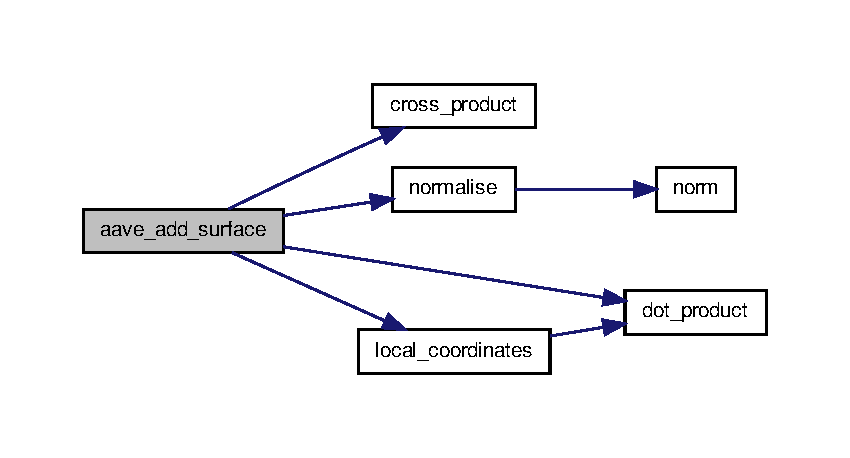
\includegraphics[width=350pt]{aave_8h_a20e98109bd38d422444f2959c0a6b80c_cgraph}
\end{center}
\end{figure}




Here is the caller graph for this function\-:\nopagebreak
\begin{figure}[H]
\begin{center}
\leavevmode
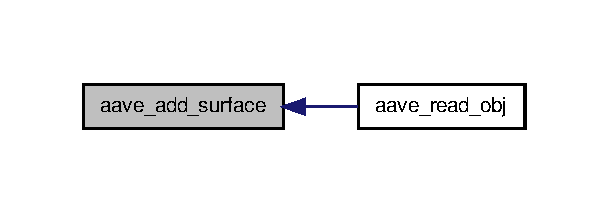
\includegraphics[width=292pt]{aave_8h_a20e98109bd38d422444f2959c0a6b80c_icgraph}
\end{center}
\end{figure}


\hypertarget{aave_8h_a8a63aae9a55200e05235e6e89990f1c6}{\index{aave.\-h@{aave.\-h}!aave\-\_\-get\-\_\-audio@{aave\-\_\-get\-\_\-audio}}
\index{aave\-\_\-get\-\_\-audio@{aave\-\_\-get\-\_\-audio}!aave.h@{aave.\-h}}
\subsubsection[{aave\-\_\-get\-\_\-audio}]{\setlength{\rightskip}{0pt plus 5cm}void aave\-\_\-get\-\_\-audio (
\begin{DoxyParamCaption}
\item[{struct {\bf aave} $\ast$}]{aave, }
\item[{short $\ast$}]{buf, }
\item[{unsigned}]{n}
\end{DoxyParamCaption}
)}}\label{aave_8h_a8a63aae9a55200e05235e6e89990f1c6}
Generate {\ttfamily n} 16-\/bit 2-\/channel frames of the auralisation world {\ttfamily aave} and put them in the memory location pointed by {\ttfamily buf}. \begin{Desc}
\item[Examples\-: ]\par
\hyperlink{examples_2circle_8c-example}{examples/circle.\-c}, \hyperlink{examples_2elevation_8c-example}{examples/elevation.\-c}, \hyperlink{examples_2line_8c-example}{examples/line.\-c}, and \hyperlink{examples_2stream_8c-example}{examples/stream.\-c}.\end{Desc}


Here is the call graph for this function\-:\nopagebreak
\begin{figure}[H]
\begin{center}
\leavevmode
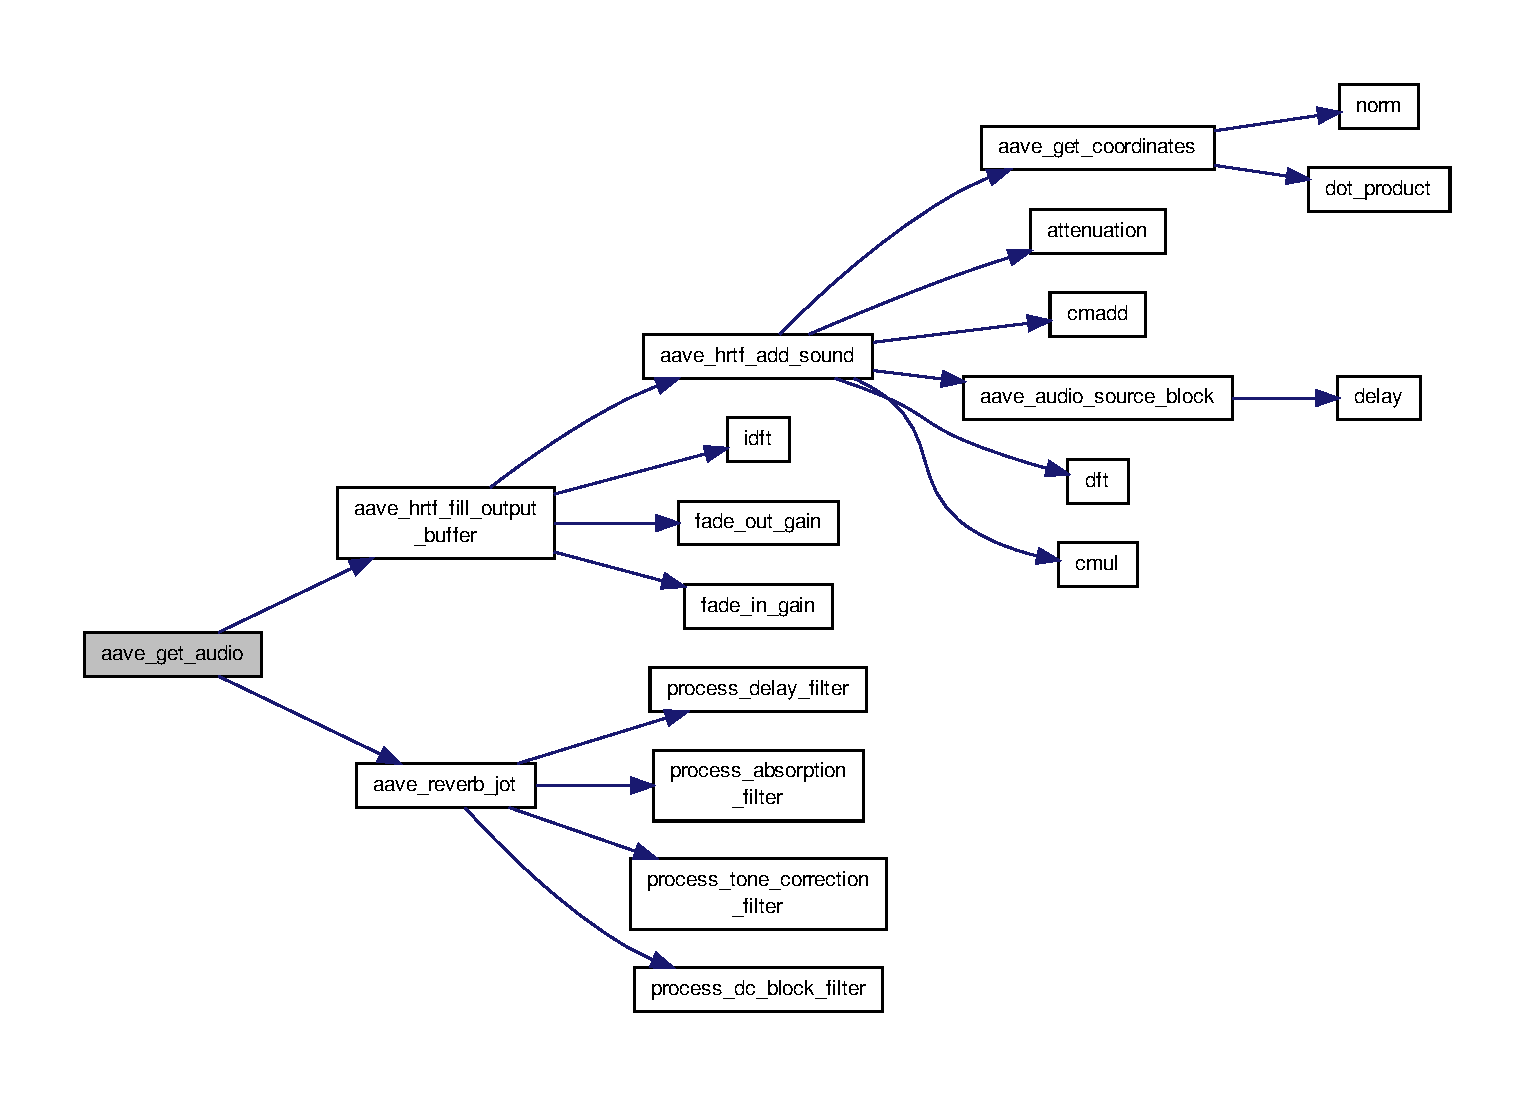
\includegraphics[width=350pt]{aave_8h_a8a63aae9a55200e05235e6e89990f1c6_cgraph}
\end{center}
\end{figure}


\hypertarget{aave_8h_a98cd836fde1ac54fc6dcbb3aab416d8b}{\index{aave.\-h@{aave.\-h}!aave\-\_\-get\-\_\-coordinates@{aave\-\_\-get\-\_\-coordinates}}
\index{aave\-\_\-get\-\_\-coordinates@{aave\-\_\-get\-\_\-coordinates}!aave.h@{aave.\-h}}
\subsubsection[{aave\-\_\-get\-\_\-coordinates}]{\setlength{\rightskip}{0pt plus 5cm}void aave\-\_\-get\-\_\-coordinates (
\begin{DoxyParamCaption}
\item[{const struct {\bf aave} $\ast$}]{aave, }
\item[{const float $\ast$}]{source\-\_\-position, }
\item[{float $\ast$}]{distance, }
\item[{float $\ast$}]{elevation, }
\item[{float $\ast$}]{azimuth}
\end{DoxyParamCaption}
)}}\label{aave_8h_a98cd836fde1ac54fc6dcbb3aab416d8b}
Get the {\ttfamily distance} (m), {\ttfamily azimuth} (rad) and {\ttfamily elevation} (rad) coordinates of the position {\ttfamily source\-\_\-position} of a source relative to the listener. 

Here is the call graph for this function\-:\nopagebreak
\begin{figure}[H]
\begin{center}
\leavevmode
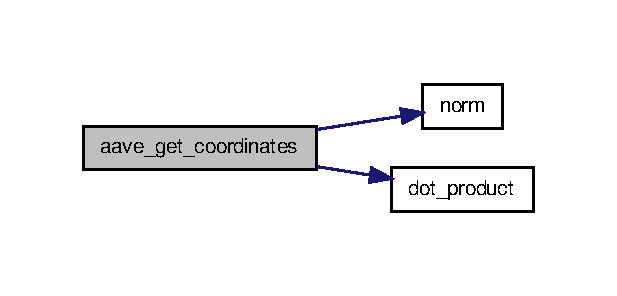
\includegraphics[width=296pt]{aave_8h_a98cd836fde1ac54fc6dcbb3aab416d8b_cgraph}
\end{center}
\end{figure}




Here is the caller graph for this function\-:\nopagebreak
\begin{figure}[H]
\begin{center}
\leavevmode
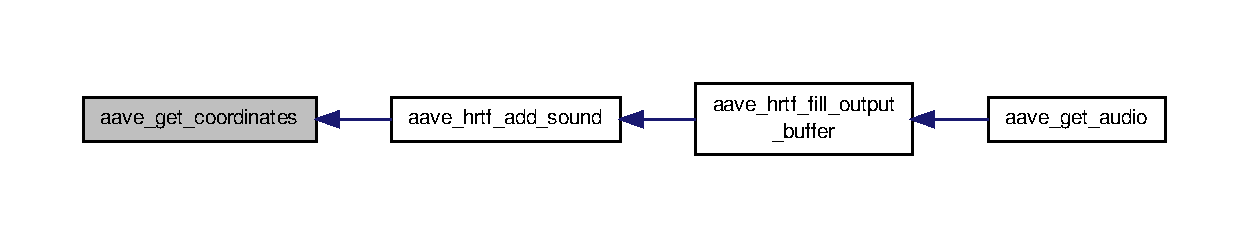
\includegraphics[width=350pt]{aave_8h_a98cd836fde1ac54fc6dcbb3aab416d8b_icgraph}
\end{center}
\end{figure}


\hypertarget{aave_8h_a952abc42265cb150fa647c008e8ee937}{\index{aave.\-h@{aave.\-h}!aave\-\_\-get\-\_\-material@{aave\-\_\-get\-\_\-material}}
\index{aave\-\_\-get\-\_\-material@{aave\-\_\-get\-\_\-material}!aave.h@{aave.\-h}}
\subsubsection[{aave\-\_\-get\-\_\-material}]{\setlength{\rightskip}{0pt plus 5cm}struct {\bf aave\-\_\-material}$\ast$ aave\-\_\-get\-\_\-material (
\begin{DoxyParamCaption}
\item[{const char $\ast$}]{name}
\end{DoxyParamCaption}
)}}\label{aave_8h_a952abc42265cb150fa647c008e8ee937}
Return the material with the specified {\ttfamily name}. If no material is found with such name, return aave\-\_\-material\-\_\-none.

The search is performed using the binary search algorithm (\href{http://en.wikipedia.org/wiki/Binary_search_algorithm}{\tt http\-://en.\-wikipedia.\-org/wiki/\-Binary\-\_\-search\-\_\-algorithm}), that's why the table of materials must be ordered by name. 

Here is the caller graph for this function\-:\nopagebreak
\begin{figure}[H]
\begin{center}
\leavevmode
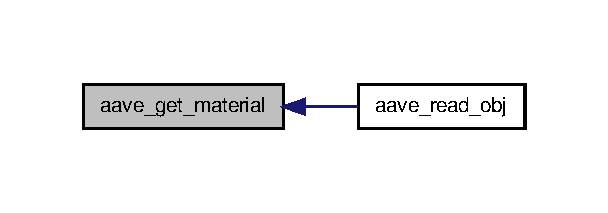
\includegraphics[width=292pt]{aave_8h_a952abc42265cb150fa647c008e8ee937_icgraph}
\end{center}
\end{figure}


\hypertarget{aave_8h_a300799824871774e895676f347905cf3}{\index{aave.\-h@{aave.\-h}!aave\-\_\-get\-\_\-material\-\_\-filter@{aave\-\_\-get\-\_\-material\-\_\-filter}}
\index{aave\-\_\-get\-\_\-material\-\_\-filter@{aave\-\_\-get\-\_\-material\-\_\-filter}!aave.h@{aave.\-h}}
\subsubsection[{aave\-\_\-get\-\_\-material\-\_\-filter}]{\setlength{\rightskip}{0pt plus 5cm}void aave\-\_\-get\-\_\-material\-\_\-filter (
\begin{DoxyParamCaption}
\item[{struct {\bf aave} $\ast$}]{aave, }
\item[{struct {\bf aave\-\_\-surface} $\ast$$\ast$}]{surfaces, }
\item[{unsigned}]{reflections, }
\item[{float $\ast$}]{filter}
\end{DoxyParamCaption}
)}}\label{aave_8h_a300799824871774e895676f347905cf3}
Design the material absorption filter for the specified sequence of {\ttfamily surfaces} and reflection order {\ttfamily reflections}. The calculated D\-F\-T coefficients of the filter are stored in {\ttfamily filter}, which must have 4 times the elements of the H\-R\-I\-Rs of the H\-R\-T\-F set currently in use. 

Here is the call graph for this function\-:\nopagebreak
\begin{figure}[H]
\begin{center}
\leavevmode
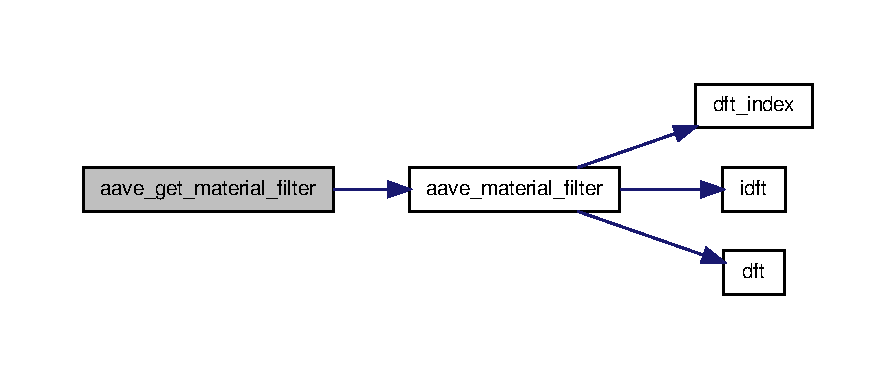
\includegraphics[width=350pt]{aave_8h_a300799824871774e895676f347905cf3_cgraph}
\end{center}
\end{figure}




Here is the caller graph for this function\-:\nopagebreak
\begin{figure}[H]
\begin{center}
\leavevmode
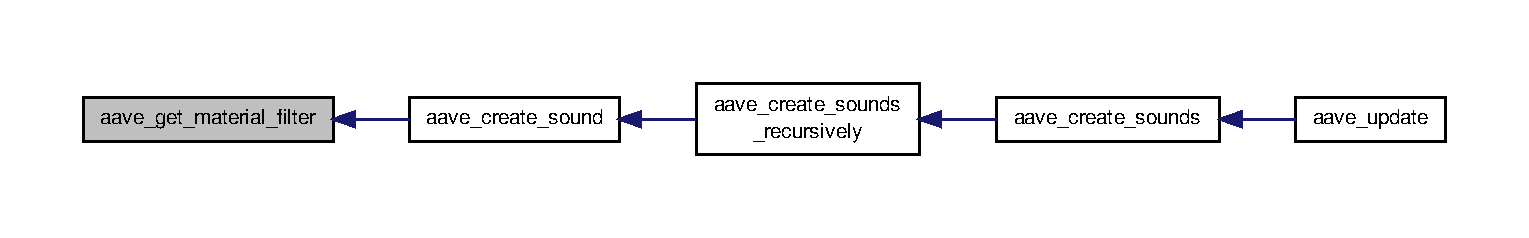
\includegraphics[width=350pt]{aave_8h_a300799824871774e895676f347905cf3_icgraph}
\end{center}
\end{figure}


\hypertarget{aave_8h_a9332f29f538c0e54272f61de0e420348}{\index{aave.\-h@{aave.\-h}!aave\-\_\-hrtf\-\_\-cipic@{aave\-\_\-hrtf\-\_\-cipic}}
\index{aave\-\_\-hrtf\-\_\-cipic@{aave\-\_\-hrtf\-\_\-cipic}!aave.h@{aave.\-h}}
\subsubsection[{aave\-\_\-hrtf\-\_\-cipic}]{\setlength{\rightskip}{0pt plus 5cm}void aave\-\_\-hrtf\-\_\-cipic (
\begin{DoxyParamCaption}
\item[{struct {\bf aave} $\ast$}]{a}
\end{DoxyParamCaption}
)}}\label{aave_8h_a9332f29f538c0e54272f61de0e420348}
Select the C\-I\-P\-I\-C H\-R\-T\-F set for the auralisation process. 

Here is the call graph for this function\-:\nopagebreak
\begin{figure}[H]
\begin{center}
\leavevmode
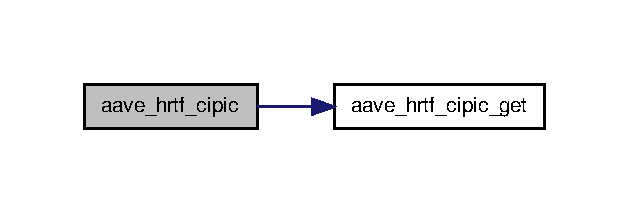
\includegraphics[width=302pt]{aave_8h_a9332f29f538c0e54272f61de0e420348_cgraph}
\end{center}
\end{figure}


\hypertarget{aave_8h_a1714770c36978ec1bfc9b4b5148e42be}{\index{aave.\-h@{aave.\-h}!aave\-\_\-hrtf\-\_\-listen@{aave\-\_\-hrtf\-\_\-listen}}
\index{aave\-\_\-hrtf\-\_\-listen@{aave\-\_\-hrtf\-\_\-listen}!aave.h@{aave.\-h}}
\subsubsection[{aave\-\_\-hrtf\-\_\-listen}]{\setlength{\rightskip}{0pt plus 5cm}void aave\-\_\-hrtf\-\_\-listen (
\begin{DoxyParamCaption}
\item[{struct {\bf aave} $\ast$}]{a}
\end{DoxyParamCaption}
)}}\label{aave_8h_a1714770c36978ec1bfc9b4b5148e42be}
Select the L\-I\-S\-T\-E\-N H\-R\-T\-F set for the auralisation process. 

Here is the call graph for this function\-:\nopagebreak
\begin{figure}[H]
\begin{center}
\leavevmode
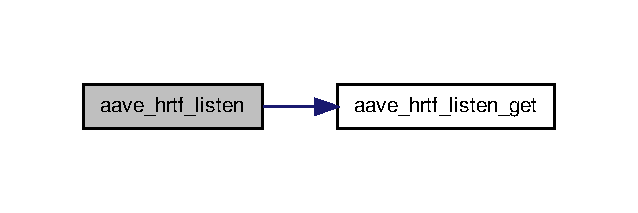
\includegraphics[width=306pt]{aave_8h_a1714770c36978ec1bfc9b4b5148e42be_cgraph}
\end{center}
\end{figure}


\hypertarget{aave_8h_aad4aa8bf733bedef0ee981bbeffc1b12}{\index{aave.\-h@{aave.\-h}!aave\-\_\-hrtf\-\_\-mit@{aave\-\_\-hrtf\-\_\-mit}}
\index{aave\-\_\-hrtf\-\_\-mit@{aave\-\_\-hrtf\-\_\-mit}!aave.h@{aave.\-h}}
\subsubsection[{aave\-\_\-hrtf\-\_\-mit}]{\setlength{\rightskip}{0pt plus 5cm}void aave\-\_\-hrtf\-\_\-mit (
\begin{DoxyParamCaption}
\item[{struct {\bf aave} $\ast$}]{a}
\end{DoxyParamCaption}
)}}\label{aave_8h_aad4aa8bf733bedef0ee981bbeffc1b12}
Select the M\-I\-T K\-E\-M\-A\-R H\-R\-T\-F compact set for the auralisation process. \begin{Desc}
\item[Examples\-: ]\par
\hyperlink{examples_2circle_8c-example}{examples/circle.\-c}, \hyperlink{examples_2elevation_8c-example}{examples/elevation.\-c}, \hyperlink{examples_2line_8c-example}{examples/line.\-c}, and \hyperlink{examples_2stream_8c-example}{examples/stream.\-c}.\end{Desc}


Here is the call graph for this function\-:\nopagebreak
\begin{figure}[H]
\begin{center}
\leavevmode
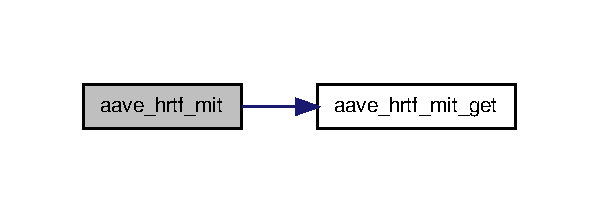
\includegraphics[width=288pt]{aave_8h_aad4aa8bf733bedef0ee981bbeffc1b12_cgraph}
\end{center}
\end{figure}


\hypertarget{aave_8h_afbc85e87d1aaab2c91c7f15d1d5a9906}{\index{aave.\-h@{aave.\-h}!aave\-\_\-hrtf\-\_\-tub@{aave\-\_\-hrtf\-\_\-tub}}
\index{aave\-\_\-hrtf\-\_\-tub@{aave\-\_\-hrtf\-\_\-tub}!aave.h@{aave.\-h}}
\subsubsection[{aave\-\_\-hrtf\-\_\-tub}]{\setlength{\rightskip}{0pt plus 5cm}void aave\-\_\-hrtf\-\_\-tub (
\begin{DoxyParamCaption}
\item[{struct {\bf aave} $\ast$}]{a}
\end{DoxyParamCaption}
)}}\label{aave_8h_afbc85e87d1aaab2c91c7f15d1d5a9906}
Select the T\-U-\/\-Berlin H\-R\-T\-F set for the auralisation process. 

Here is the call graph for this function\-:\nopagebreak
\begin{figure}[H]
\begin{center}
\leavevmode
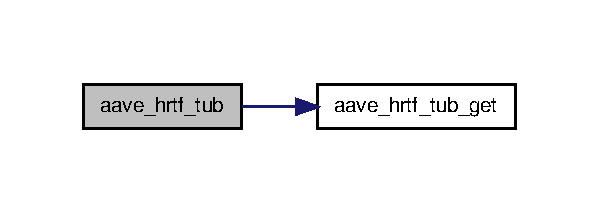
\includegraphics[width=288pt]{aave_8h_afbc85e87d1aaab2c91c7f15d1d5a9906_cgraph}
\end{center}
\end{figure}


\hypertarget{aave_8h_a044e13c0826108a728f0b6324c23fbab}{\index{aave.\-h@{aave.\-h}!aave\-\_\-init@{aave\-\_\-init}}
\index{aave\-\_\-init@{aave\-\_\-init}!aave.h@{aave.\-h}}
\subsubsection[{aave\-\_\-init}]{\setlength{\rightskip}{0pt plus 5cm}void aave\-\_\-init (
\begin{DoxyParamCaption}
\item[{struct {\bf aave} $\ast$}]{aave, }
\item[{unsigned}]{rt60}
\end{DoxyParamCaption}
)}}\label{aave_8h_a044e13c0826108a728f0b6324c23fbab}
Initialise the auralisation data structure.

The listener's initial position is (0, 0, 0).

The listener's head initial orientation is invalid! You must call \hyperlink{aave_8h_aee300969973298dab868f91f7b94724d}{aave\-\_\-set\-\_\-listener\-\_\-orientation()}!

The initial output gain is 1 (0d\-B).

The artificial reverberation tail is initially enabled. \begin{Desc}
\item[Examples\-: ]\par
\hyperlink{examples_2circle_8c-example}{examples/circle.\-c}, \hyperlink{examples_2elevation_8c-example}{examples/elevation.\-c}, \hyperlink{examples_2line_8c-example}{examples/line.\-c}, and \hyperlink{examples_2stream_8c-example}{examples/stream.\-c}.\end{Desc}


Here is the call graph for this function\-:\nopagebreak
\begin{figure}[H]
\begin{center}
\leavevmode
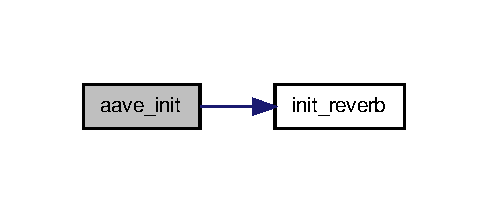
\includegraphics[width=234pt]{aave_8h_a044e13c0826108a728f0b6324c23fbab_cgraph}
\end{center}
\end{figure}


\hypertarget{aave_8h_a3682cd98f3556ad2b8c8e0bc8502371c}{\index{aave.\-h@{aave.\-h}!aave\-\_\-init\-\_\-source@{aave\-\_\-init\-\_\-source}}
\index{aave\-\_\-init\-\_\-source@{aave\-\_\-init\-\_\-source}!aave.h@{aave.\-h}}
\subsubsection[{aave\-\_\-init\-\_\-source}]{\setlength{\rightskip}{0pt plus 5cm}void aave\-\_\-init\-\_\-source (
\begin{DoxyParamCaption}
\item[{struct {\bf aave} $\ast$}]{aave, }
\item[{struct {\bf aave\-\_\-source} $\ast$}]{source}
\end{DoxyParamCaption}
)}}\label{aave_8h_a3682cd98f3556ad2b8c8e0bc8502371c}
Initialise a sound source data structure to be used by the aave engine. \begin{Desc}
\item[Examples\-: ]\par
\hyperlink{examples_2circle_8c-example}{examples/circle.\-c}, \hyperlink{examples_2elevation_8c-example}{examples/elevation.\-c}, \hyperlink{examples_2line_8c-example}{examples/line.\-c}, and \hyperlink{examples_2stream_8c-example}{examples/stream.\-c}.\end{Desc}
\hypertarget{aave_8h_a546bf3fff8b9009ddc744a6908154f5e}{\index{aave.\-h@{aave.\-h}!aave\-\_\-put\-\_\-audio@{aave\-\_\-put\-\_\-audio}}
\index{aave\-\_\-put\-\_\-audio@{aave\-\_\-put\-\_\-audio}!aave.h@{aave.\-h}}
\subsubsection[{aave\-\_\-put\-\_\-audio}]{\setlength{\rightskip}{0pt plus 5cm}void aave\-\_\-put\-\_\-audio (
\begin{DoxyParamCaption}
\item[{struct {\bf aave\-\_\-source} $\ast$}]{source, }
\item[{const short $\ast$}]{audio, }
\item[{unsigned}]{n}
\end{DoxyParamCaption}
)}}\label{aave_8h_a546bf3fff8b9009ddc744a6908154f5e}
Put the {\ttfamily n} frames pointed by {\ttfamily audio} in the ring buffer of {\ttfamily source}. \begin{Desc}
\item[Examples\-: ]\par
\hyperlink{examples_2circle_8c-example}{examples/circle.\-c}, \hyperlink{examples_2elevation_8c-example}{examples/elevation.\-c}, \hyperlink{examples_2line_8c-example}{examples/line.\-c}, and \hyperlink{examples_2stream_8c-example}{examples/stream.\-c}.\end{Desc}
\hypertarget{aave_8h_a7e664852f336438524336bdcac8be8bc}{\index{aave.\-h@{aave.\-h}!aave\-\_\-read\-\_\-obj@{aave\-\_\-read\-\_\-obj}}
\index{aave\-\_\-read\-\_\-obj@{aave\-\_\-read\-\_\-obj}!aave.h@{aave.\-h}}
\subsubsection[{aave\-\_\-read\-\_\-obj}]{\setlength{\rightskip}{0pt plus 5cm}void aave\-\_\-read\-\_\-obj (
\begin{DoxyParamCaption}
\item[{struct {\bf aave} $\ast$}]{aave, }
\item[{const char $\ast$}]{filename, }
\item[{unsigned}]{volume, }
\item[{unsigned}]{area}
\end{DoxyParamCaption}
)}}\label{aave_8h_a7e664852f336438524336bdcac8be8bc}
Read the .obj file {\ttfamily filename} and add its contents to the auralisation engine {\ttfamily aave}. \begin{Desc}
\item[Examples\-: ]\par
\hyperlink{examples_2line_8c-example}{examples/line.\-c}, and \hyperlink{examples_2stream_8c-example}{examples/stream.\-c}.\end{Desc}


Here is the call graph for this function\-:\nopagebreak
\begin{figure}[H]
\begin{center}
\leavevmode
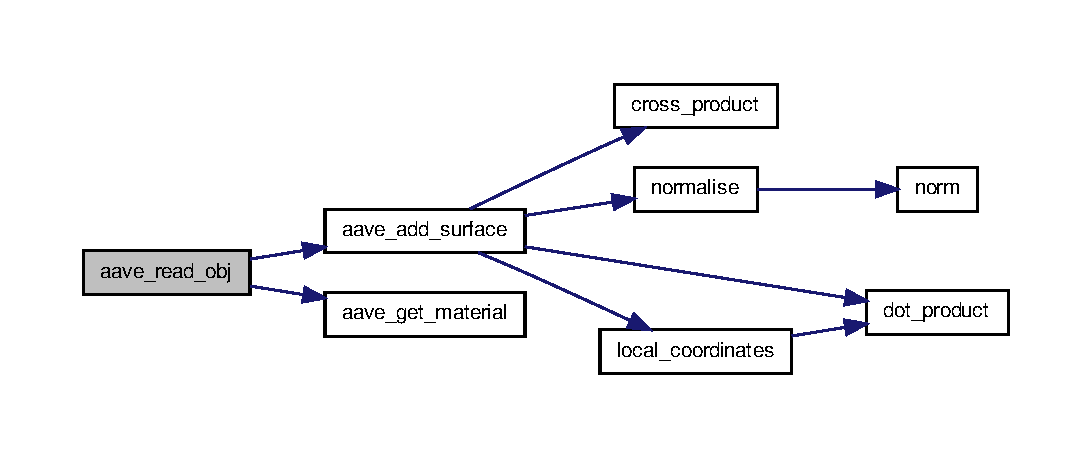
\includegraphics[width=350pt]{aave_8h_a7e664852f336438524336bdcac8be8bc_cgraph}
\end{center}
\end{figure}


\hypertarget{aave_8h_a87108aa6128bb303f58c46307a4b4ebb}{\index{aave.\-h@{aave.\-h}!aave\-\_\-reverb\-\_\-dattorro@{aave\-\_\-reverb\-\_\-dattorro}}
\index{aave\-\_\-reverb\-\_\-dattorro@{aave\-\_\-reverb\-\_\-dattorro}!aave.h@{aave.\-h}}
\subsubsection[{aave\-\_\-reverb\-\_\-dattorro}]{\setlength{\rightskip}{0pt plus 5cm}void aave\-\_\-reverb\-\_\-dattorro (
\begin{DoxyParamCaption}
\item[{struct {\bf aave} $\ast$}]{aave, }
\item[{short $\ast$}]{audio, }
\item[{unsigned}]{n}
\end{DoxyParamCaption}
)}}\label{aave_8h_a87108aa6128bb303f58c46307a4b4ebb}
Run a Dattorro reverberator to add an artificial reverberation tail to the {\ttfamily n} binaural frames (2 $\ast$ {\ttfamily n} samples) pointed by {\ttfamily audio}. 

Here is the call graph for this function\-:\nopagebreak
\begin{figure}[H]
\begin{center}
\leavevmode
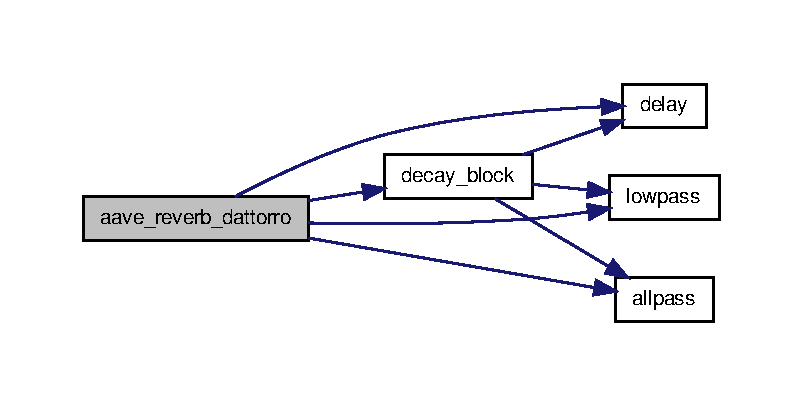
\includegraphics[width=350pt]{aave_8h_a87108aa6128bb303f58c46307a4b4ebb_cgraph}
\end{center}
\end{figure}


\hypertarget{aave_8h_aa5850eee4b27f5b7f2732f3457e00d79}{\index{aave.\-h@{aave.\-h}!aave\-\_\-reverb\-\_\-jot@{aave\-\_\-reverb\-\_\-jot}}
\index{aave\-\_\-reverb\-\_\-jot@{aave\-\_\-reverb\-\_\-jot}!aave.h@{aave.\-h}}
\subsubsection[{aave\-\_\-reverb\-\_\-jot}]{\setlength{\rightskip}{0pt plus 5cm}void aave\-\_\-reverb\-\_\-jot (
\begin{DoxyParamCaption}
\item[{struct {\bf aave} $\ast$}]{aave, }
\item[{short $\ast$}]{audio, }
\item[{unsigned}]{n}
\end{DoxyParamCaption}
)}}\label{aave_8h_aa5850eee4b27f5b7f2732f3457e00d79}
Run a Jot F\-D\-N reverberator to add an artificial reverberation tail to the {\ttfamily n} single channel frames ({\ttfamily n} samples) of each anechoic sound source pointed by {\ttfamily aave-\/$>$sources}. Store output in {\ttfamily audio}. 

Here is the call graph for this function\-:\nopagebreak
\begin{figure}[H]
\begin{center}
\leavevmode
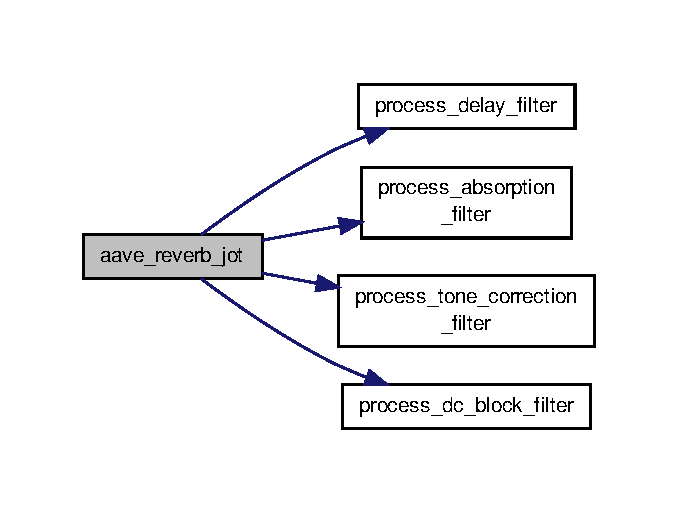
\includegraphics[width=326pt]{aave_8h_aa5850eee4b27f5b7f2732f3457e00d79_cgraph}
\end{center}
\end{figure}




Here is the caller graph for this function\-:\nopagebreak
\begin{figure}[H]
\begin{center}
\leavevmode
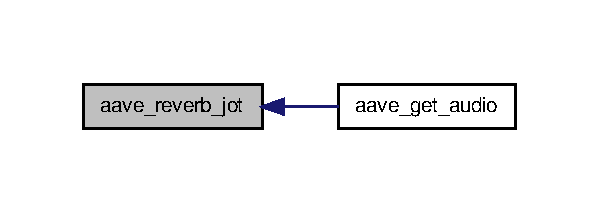
\includegraphics[width=288pt]{aave_8h_aa5850eee4b27f5b7f2732f3457e00d79_icgraph}
\end{center}
\end{figure}


\hypertarget{aave_8h_aee300969973298dab868f91f7b94724d}{\index{aave.\-h@{aave.\-h}!aave\-\_\-set\-\_\-listener\-\_\-orientation@{aave\-\_\-set\-\_\-listener\-\_\-orientation}}
\index{aave\-\_\-set\-\_\-listener\-\_\-orientation@{aave\-\_\-set\-\_\-listener\-\_\-orientation}!aave.h@{aave.\-h}}
\subsubsection[{aave\-\_\-set\-\_\-listener\-\_\-orientation}]{\setlength{\rightskip}{0pt plus 5cm}void aave\-\_\-set\-\_\-listener\-\_\-orientation (
\begin{DoxyParamCaption}
\item[{struct {\bf aave} $\ast$}]{aave, }
\item[{float}]{roll, }
\item[{float}]{pitch, }
\item[{float}]{yaw}
\end{DoxyParamCaption}
)}}\label{aave_8h_aee300969973298dab868f91f7b94724d}
Set the orientation of the listener's head. \begin{Desc}
\item[Examples\-: ]\par
\hyperlink{examples_2circle_8c-example}{examples/circle.\-c}, \hyperlink{examples_2elevation_8c-example}{examples/elevation.\-c}, \hyperlink{examples_2line_8c-example}{examples/line.\-c}, and \hyperlink{examples_2stream_8c-example}{examples/stream.\-c}.\end{Desc}
\hypertarget{aave_8h_a41a4224263cd8432d79099871d542b2e}{\index{aave.\-h@{aave.\-h}!aave\-\_\-set\-\_\-listener\-\_\-position@{aave\-\_\-set\-\_\-listener\-\_\-position}}
\index{aave\-\_\-set\-\_\-listener\-\_\-position@{aave\-\_\-set\-\_\-listener\-\_\-position}!aave.h@{aave.\-h}}
\subsubsection[{aave\-\_\-set\-\_\-listener\-\_\-position}]{\setlength{\rightskip}{0pt plus 5cm}void aave\-\_\-set\-\_\-listener\-\_\-position (
\begin{DoxyParamCaption}
\item[{struct {\bf aave} $\ast$}]{aave, }
\item[{float}]{x, }
\item[{float}]{y, }
\item[{float}]{z}
\end{DoxyParamCaption}
)}}\label{aave_8h_a41a4224263cd8432d79099871d542b2e}
Set the position of the listener.

The \hyperlink{aave_8h_a5acfa7c6e7e714ff364cda9dabd7a2f8}{aave\-\_\-update()} function should be called afterwards to update the state of the auralisation engine to reflect the new position. \begin{Desc}
\item[Examples\-: ]\par
\hyperlink{examples_2circle_8c-example}{examples/circle.\-c}, \hyperlink{examples_2elevation_8c-example}{examples/elevation.\-c}, \hyperlink{examples_2line_8c-example}{examples/line.\-c}, and \hyperlink{examples_2stream_8c-example}{examples/stream.\-c}.\end{Desc}
\hypertarget{aave_8h_ad48ffc19be78794acb7bf0f9a6397c11}{\index{aave.\-h@{aave.\-h}!aave\-\_\-set\-\_\-source\-\_\-position@{aave\-\_\-set\-\_\-source\-\_\-position}}
\index{aave\-\_\-set\-\_\-source\-\_\-position@{aave\-\_\-set\-\_\-source\-\_\-position}!aave.h@{aave.\-h}}
\subsubsection[{aave\-\_\-set\-\_\-source\-\_\-position}]{\setlength{\rightskip}{0pt plus 5cm}void aave\-\_\-set\-\_\-source\-\_\-position (
\begin{DoxyParamCaption}
\item[{struct {\bf aave\-\_\-source} $\ast$}]{source, }
\item[{float}]{x, }
\item[{float}]{y, }
\item[{float}]{z}
\end{DoxyParamCaption}
)}}\label{aave_8h_ad48ffc19be78794acb7bf0f9a6397c11}
Set the position of a sound source.

The \hyperlink{aave_8h_a5acfa7c6e7e714ff364cda9dabd7a2f8}{aave\-\_\-update()} function should be called afterwards to update the state of the auralisation engine to reflect the new position. \begin{Desc}
\item[Examples\-: ]\par
\hyperlink{examples_2circle_8c-example}{examples/circle.\-c}, \hyperlink{examples_2elevation_8c-example}{examples/elevation.\-c}, \hyperlink{examples_2line_8c-example}{examples/line.\-c}, and \hyperlink{examples_2stream_8c-example}{examples/stream.\-c}.\end{Desc}
\hypertarget{aave_8h_a5acfa7c6e7e714ff364cda9dabd7a2f8}{\index{aave.\-h@{aave.\-h}!aave\-\_\-update@{aave\-\_\-update}}
\index{aave\-\_\-update@{aave\-\_\-update}!aave.h@{aave.\-h}}
\subsubsection[{aave\-\_\-update}]{\setlength{\rightskip}{0pt plus 5cm}void aave\-\_\-update (
\begin{DoxyParamCaption}
\item[{struct {\bf aave} $\ast$}]{aave}
\end{DoxyParamCaption}
)}}\label{aave_8h_a5acfa7c6e7e714ff364cda9dabd7a2f8}
Update the whole state of the auralisation world. Runs the visibility checks for all sounds from all sources. \begin{Desc}
\item[Examples\-: ]\par
\hyperlink{examples_2circle_8c-example}{examples/circle.\-c}, \hyperlink{examples_2elevation_8c-example}{examples/elevation.\-c}, \hyperlink{examples_2line_8c-example}{examples/line.\-c}, and \hyperlink{examples_2stream_8c-example}{examples/stream.\-c}.\end{Desc}


Here is the call graph for this function\-:\nopagebreak
\begin{figure}[H]
\begin{center}
\leavevmode
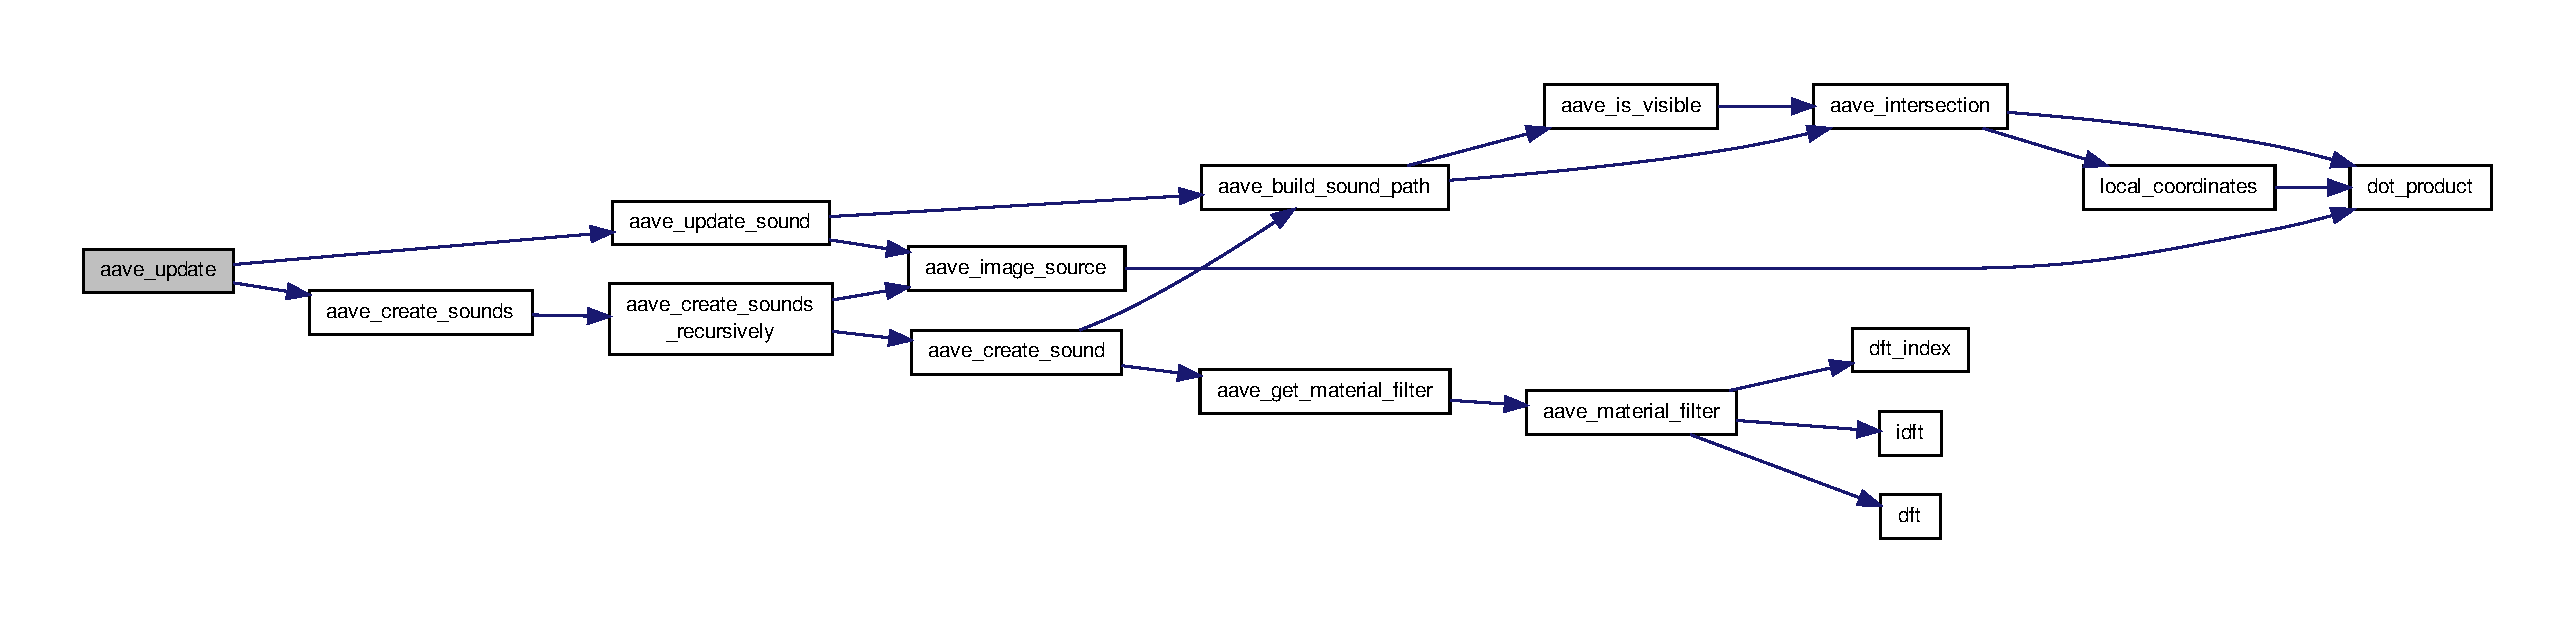
\includegraphics[width=350pt]{aave_8h_a5acfa7c6e7e714ff364cda9dabd7a2f8_cgraph}
\end{center}
\end{figure}


\hypertarget{aave_8h_a5b453c8df5597105b3a7cde336e83e0e}{\index{aave.\-h@{aave.\-h}!dft\-\_\-index@{dft\-\_\-index}}
\index{dft\-\_\-index@{dft\-\_\-index}!aave.h@{aave.\-h}}
\subsubsection[{dft\-\_\-index}]{\setlength{\rightskip}{0pt plus 5cm}unsigned dft\-\_\-index (
\begin{DoxyParamCaption}
\item[{unsigned}]{i, }
\item[{unsigned}]{n}
\end{DoxyParamCaption}
)}}\label{aave_8h_a5b453c8df5597105b3a7cde336e83e0e}
This function returns the index into the D\-F\-T data calculated by \hyperlink{dft_8h_ad9584a3bdc946bf6faece23f05dc797d}{dft()} that contains the Fourier coefficient {\ttfamily i} for a D\-F\-T of size {\ttfamily n}. {\ttfamily n} is a power of 2, up to the maximum supported by dft\-\_\-index\-\_\-table (currently 128). {\ttfamily i} is a value from 0 up to {\ttfamily n} / 2 -\/ 1, since the input data is real\-:
\begin{DoxyItemize}
\item X\mbox{[}0\mbox{]} = X\mbox{[}0\mbox{]}.real; X\mbox{[}0\mbox{]}.imag = 0;
\item X\mbox{[}1\mbox{]} = X\mbox{[}N/2\mbox{]}.real; X\mbox{[}N/2\mbox{]}.imag = 0;
\item X\mbox{[}N/2+i\mbox{]}.real = X\mbox{[}N/2-\/i\mbox{]}.real;
\item X\mbox{[}N/2+i\mbox{]}.imag = -\/ X\mbox{[}N/2-\/i\mbox{]}.imag; 
\end{DoxyItemize}

Here is the caller graph for this function\-:\nopagebreak
\begin{figure}[H]
\begin{center}
\leavevmode
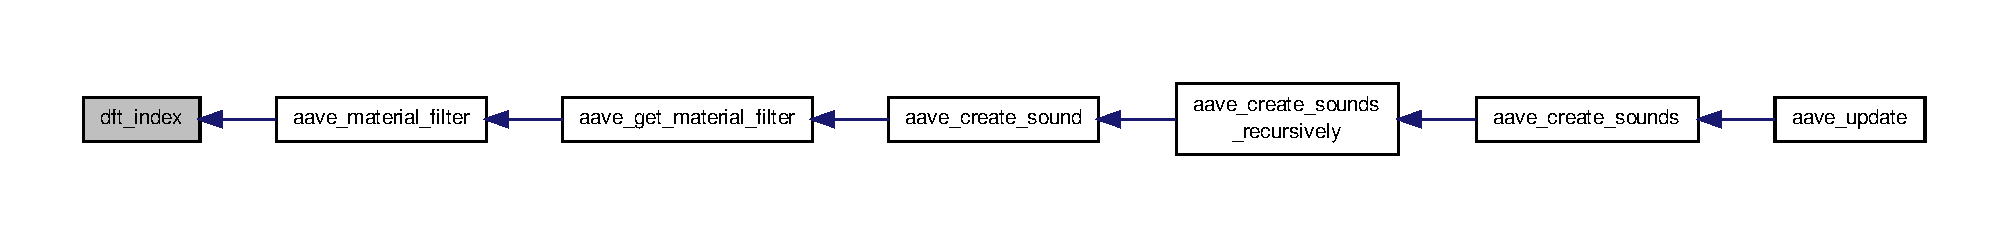
\includegraphics[width=350pt]{aave_8h_a5b453c8df5597105b3a7cde336e83e0e_icgraph}
\end{center}
\end{figure}


\hypertarget{aave_8h_a08e9496e914691f6f87708b74992020e}{\index{aave.\-h@{aave.\-h}!init\-\_\-reverb@{init\-\_\-reverb}}
\index{init\-\_\-reverb@{init\-\_\-reverb}!aave.h@{aave.\-h}}
\subsubsection[{init\-\_\-reverb}]{\setlength{\rightskip}{0pt plus 5cm}void init\-\_\-reverb (
\begin{DoxyParamCaption}
\item[{struct {\bf aave\-\_\-reverb} $\ast$}]{reverb, }
\item[{float}]{volume, }
\item[{float}]{area, }
\item[{float}]{abs}
\end{DoxyParamCaption}
)}}\label{aave_8h_a08e9496e914691f6f87708b74992020e}
Initialize reverb parameters. 

Here is the caller graph for this function\-:\nopagebreak
\begin{figure}[H]
\begin{center}
\leavevmode
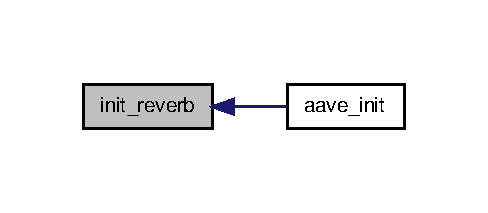
\includegraphics[width=234pt]{aave_8h_a08e9496e914691f6f87708b74992020e_icgraph}
\end{center}
\end{figure}




\subsection{Variable Documentation}
\hypertarget{aave_8h_a49ce2ac99af8e6a499e6b6dfa8962e58}{\index{aave.\-h@{aave.\-h}!aave\-\_\-material\-\_\-none@{aave\-\_\-material\-\_\-none}}
\index{aave\-\_\-material\-\_\-none@{aave\-\_\-material\-\_\-none}!aave.h@{aave.\-h}}
\subsubsection[{aave\-\_\-material\-\_\-none}]{\setlength{\rightskip}{0pt plus 5cm}struct {\bf aave\-\_\-material} aave\-\_\-material\-\_\-none}}\label{aave_8h_a49ce2ac99af8e6a499e6b6dfa8962e58}
Full reflective material to use when no material is specified for a surface, or when the specified material is not found in aave\-\_\-materials. 
\hypertarget{audio_8c}{\section{audio.\-c File Reference}
\label{audio_8c}\index{audio.\-c@{audio.\-c}}
}
{\ttfamily \#include $<$math.\-h$>$}\\*
{\ttfamily \#include $<$string.\-h$>$}\\*
{\ttfamily \#include $<$stdio.\-h$>$}\\*
{\ttfamily \#include \char`\"{}aave.\-h\char`\"{}}\\*
{\ttfamily \#include \char`\"{}dft.\-h\char`\"{}}\\*
{\ttfamily \#include \char`\"{}idft.\-h\char`\"{}}\\*
Include dependency graph for audio.\-c\-:\nopagebreak
\begin{figure}[H]
\begin{center}
\leavevmode
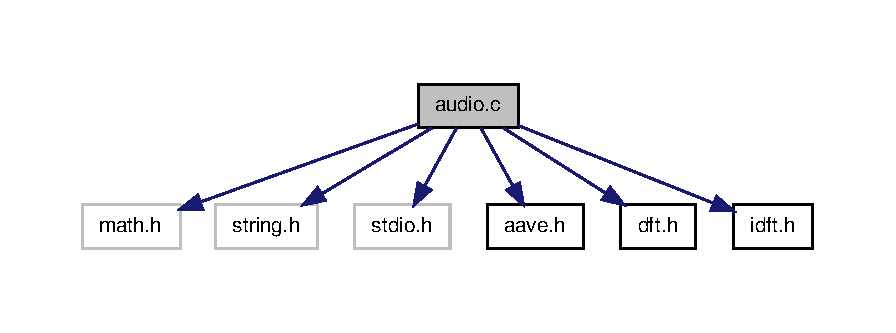
\includegraphics[width=350pt]{audio_8c__incl}
\end{center}
\end{figure}
\subsection*{Macros}
\begin{DoxyCompactItemize}
\item 
\#define \hyperlink{audio_8c_a11ddec9c2a797ebe5e6b6f2ae522404f}{D\-F\-T\-\_\-\-T\-Y\-P\-E}~short
\item 
\#define \hyperlink{audio_8c_afd47bdf71dbf8a1adbddc63efd267700}{I\-D\-F\-T\-\_\-\-T\-Y\-P\-E}~int
\item 
\#define \hyperlink{audio_8c_addce93e897e9f71ef5c263ffd893f831}{A\-A\-V\-E\-\_\-\-F\-A\-D\-E\-\_\-\-S\-A\-M\-P\-L\-E\-S}~4096
\item 
\#define \hyperlink{audio_8c_a7921e52736402cbfff73045ce89695e7}{A\-A\-V\-E\-\_\-\-D\-I\-S\-T\-A\-N\-C\-E\-\_\-\-B1}~0.\-99977
\end{DoxyCompactItemize}
\subsection*{Functions}
\begin{DoxyCompactItemize}
\item 
static float \hyperlink{audio_8c_a01cdef4fc35ac0cf58e59bed7c2af7d9}{attenuation} (float distance)
\item 
static float \hyperlink{audio_8c_a0ed45f17383de6ca52241b5ac60a10b2}{fade\-\_\-in\-\_\-gain} (unsigned i, unsigned frames)
\item 
static float \hyperlink{audio_8c_a3bff6ddd40eda3065aa82561d23e51a6}{fade\-\_\-out\-\_\-gain} (unsigned i, unsigned frames)
\item 
static void \hyperlink{audio_8c_a5949cca50430419a0d66b75f6bf5793a}{cmul} (float $\ast$a, const float $\ast$b, unsigned n)
\item 
static void \hyperlink{audio_8c_a4e6a8bd6af1e6e28fb9f4a59802913d6}{cmadd} (float $\ast$y, const float $\ast$a, const float $\ast$b, unsigned n, float g)
\item 
static void \hyperlink{audio_8c_a8dfc247d60dfeb02fe97ae7353731506}{aave\-\_\-audio\-\_\-source\-\_\-block} (struct \hyperlink{structaave__sound}{aave\-\_\-sound} $\ast$sound, float distance, short $\ast$x, unsigned frames, unsigned \hyperlink{structdelay}{delay})
\item 
static void \hyperlink{audio_8c_a74e68044085a9e60e9d9065100a520b0}{aave\-\_\-hrtf\-\_\-add\-\_\-sound} (struct \hyperlink{structaave}{aave} $\ast$\hyperlink{structaave}{aave}, struct \hyperlink{structaave__sound}{aave\-\_\-sound} $\ast$sound, float ydft\mbox{[}3\mbox{]}\mbox{[}2\mbox{]}\mbox{[}\hyperlink{aave_8h_a19ea3a18eb313fc3b825f522245d19d3}{A\-A\-V\-E\-\_\-\-M\-A\-X\-\_\-\-H\-R\-T\-F} $\ast$4\mbox{]}, unsigned \hyperlink{structdelay}{delay}, unsigned frames)
\item 
static void \hyperlink{audio_8c_a0435bc74e8d5edca85e72ab93a72bc37}{aave\-\_\-hrtf\-\_\-fill\-\_\-output\-\_\-buffer} (struct \hyperlink{structaave}{aave} $\ast$\hyperlink{structaave}{aave}, unsigned \hyperlink{structdelay}{delay}, unsigned frames)
\item 
void \hyperlink{audio_8c_afe43a0d12af335e2f133c0da2a99422f}{aave\-\_\-get\-\_\-audio} (struct \hyperlink{structaave}{aave} $\ast$\hyperlink{structaave}{aave}, short $\ast$buf, unsigned n)
\item 
void \hyperlink{audio_8c_a8652f21a39abdea73f6ad975ad7af5fd}{aave\-\_\-put\-\_\-audio} (struct \hyperlink{structaave__source}{aave\-\_\-source} $\ast$source, const short $\ast$audio, unsigned n)
\end{DoxyCompactItemize}


\subsection{Detailed Description}
The \hyperlink{audio_8c}{audio.\-c} file contains the functions that implement the core of the auralisation audio processing of the Acoustic\-A\-V\-E library (libaave). The following image illustrates the audio processing model of the library, as seen by the user.


\begin{DoxyImage}
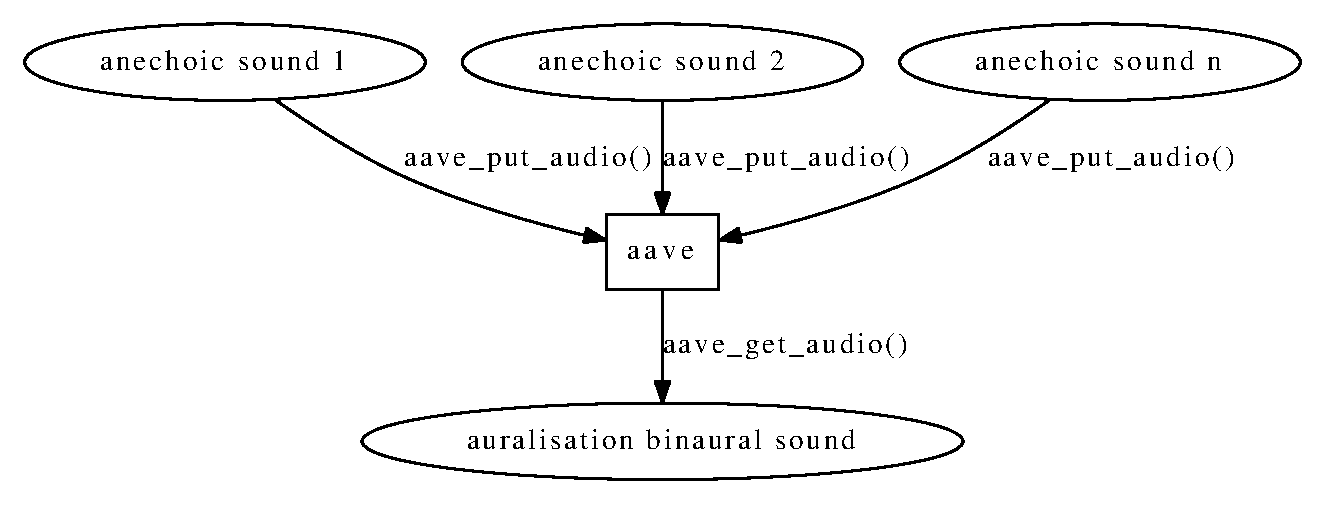
\includegraphics[width=\textwidth]{audio1}
\caption{Audio processing model}
\end{DoxyImage}


The user passes the anechoic audio data of each sound source in the auralisation world to the library using \hyperlink{aave_8h_a546bf3fff8b9009ddc744a6908154f5e}{aave\-\_\-put\-\_\-audio()} and then retrieves the calculated auralisation binaural audio data using \hyperlink{aave_8h_a8a63aae9a55200e05235e6e89990f1c6}{aave\-\_\-get\-\_\-audio()}.

Although the library supports processing one audio frame at a time, users would typically work with blocks of audio frames at a time, for efficiency reasons of the underlying operating system. Each time, the number of anechoic audio frames (samples) in the blocks passed to each source using \hyperlink{aave_8h_a546bf3fff8b9009ddc744a6908154f5e}{aave\-\_\-put\-\_\-audio()} must be the same for all sources, and the same number of binaural audio frames (samples times 2) must be retrieved using \hyperlink{aave_8h_a8a63aae9a55200e05235e6e89990f1c6}{aave\-\_\-get\-\_\-audio()}.

The current implementation of the library runs most efficiently when the number of audio frames per block is a multiple of the number of samples of the selected head-\/related transfer functions (H\-R\-T\-F), times 2, as that is the size of the discrete Fourier transforms (D\-F\-T) performed internally.

The H\-R\-T\-F set to use for the auralisation process can be selected by calling one of \hyperlink{aave_8h_a9332f29f538c0e54272f61de0e420348}{aave\-\_\-hrtf\-\_\-cipic()}, \hyperlink{aave_8h_a1714770c36978ec1bfc9b4b5148e42be}{aave\-\_\-hrtf\-\_\-listen()}, \hyperlink{aave_8h_aad4aa8bf733bedef0ee981bbeffc1b12}{aave\-\_\-hrtf\-\_\-mit()}, or \hyperlink{aave_8h_afbc85e87d1aaab2c91c7f15d1d5a9906}{aave\-\_\-hrtf\-\_\-tub()}, for the C\-I\-P\-I\-C, L\-I\-S\-T\-E\-N, M\-I\-T, or T\-U-\/\-Berlin H\-R\-T\-F sets, respectively, and it must be done before ever calling \hyperlink{aave_8h_a546bf3fff8b9009ddc744a6908154f5e}{aave\-\_\-put\-\_\-audio()}.

The following describes the internal implementation details of the audio processing performed by the library to produce the auralisation. Mere users of the library may want to skip the rest of this section.


\begin{DoxyImage}
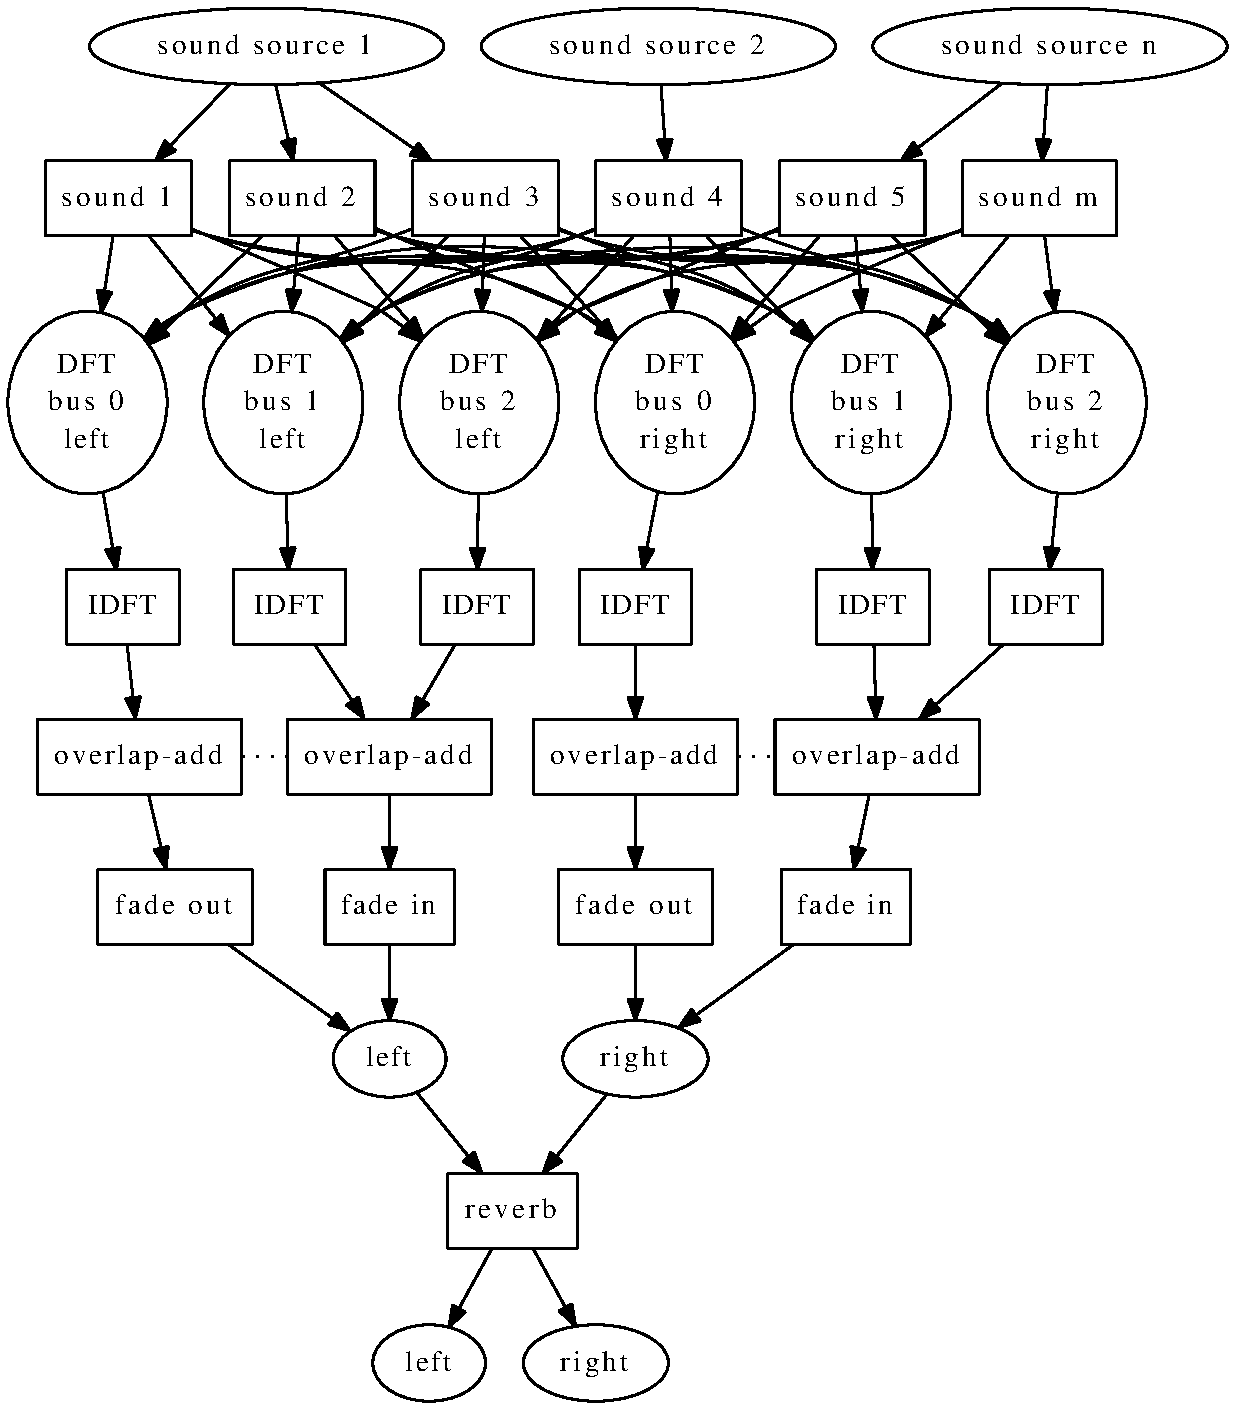
\includegraphics[width=\textwidth]{audio2}
\caption{Overall audio processing block diagram}
\end{DoxyImage}


The above image illustrates the entire auralisation audio processing, performed by \hyperlink{aave_8h_a8a63aae9a55200e05235e6e89990f1c6}{aave\-\_\-get\-\_\-audio()}, from the anechoic audio data of all sound sources present, to the resulting auralisation left and right (binaural) audio data.

Each sound source originates a number of sounds that reach the listener (direct sound and reflection sounds, as many as the \hyperlink{geometry_8c}{geometry.\-c} part of the auralisation process is able to find in a given amount of time). Each sound is processed differently according to the travelled distance, direction of arrival, and materials of the reflection surfaces, mainly. This audio processing is represented by the sound-\/i boxes in the image above and is further expanded in the image below.


\begin{DoxyImage}
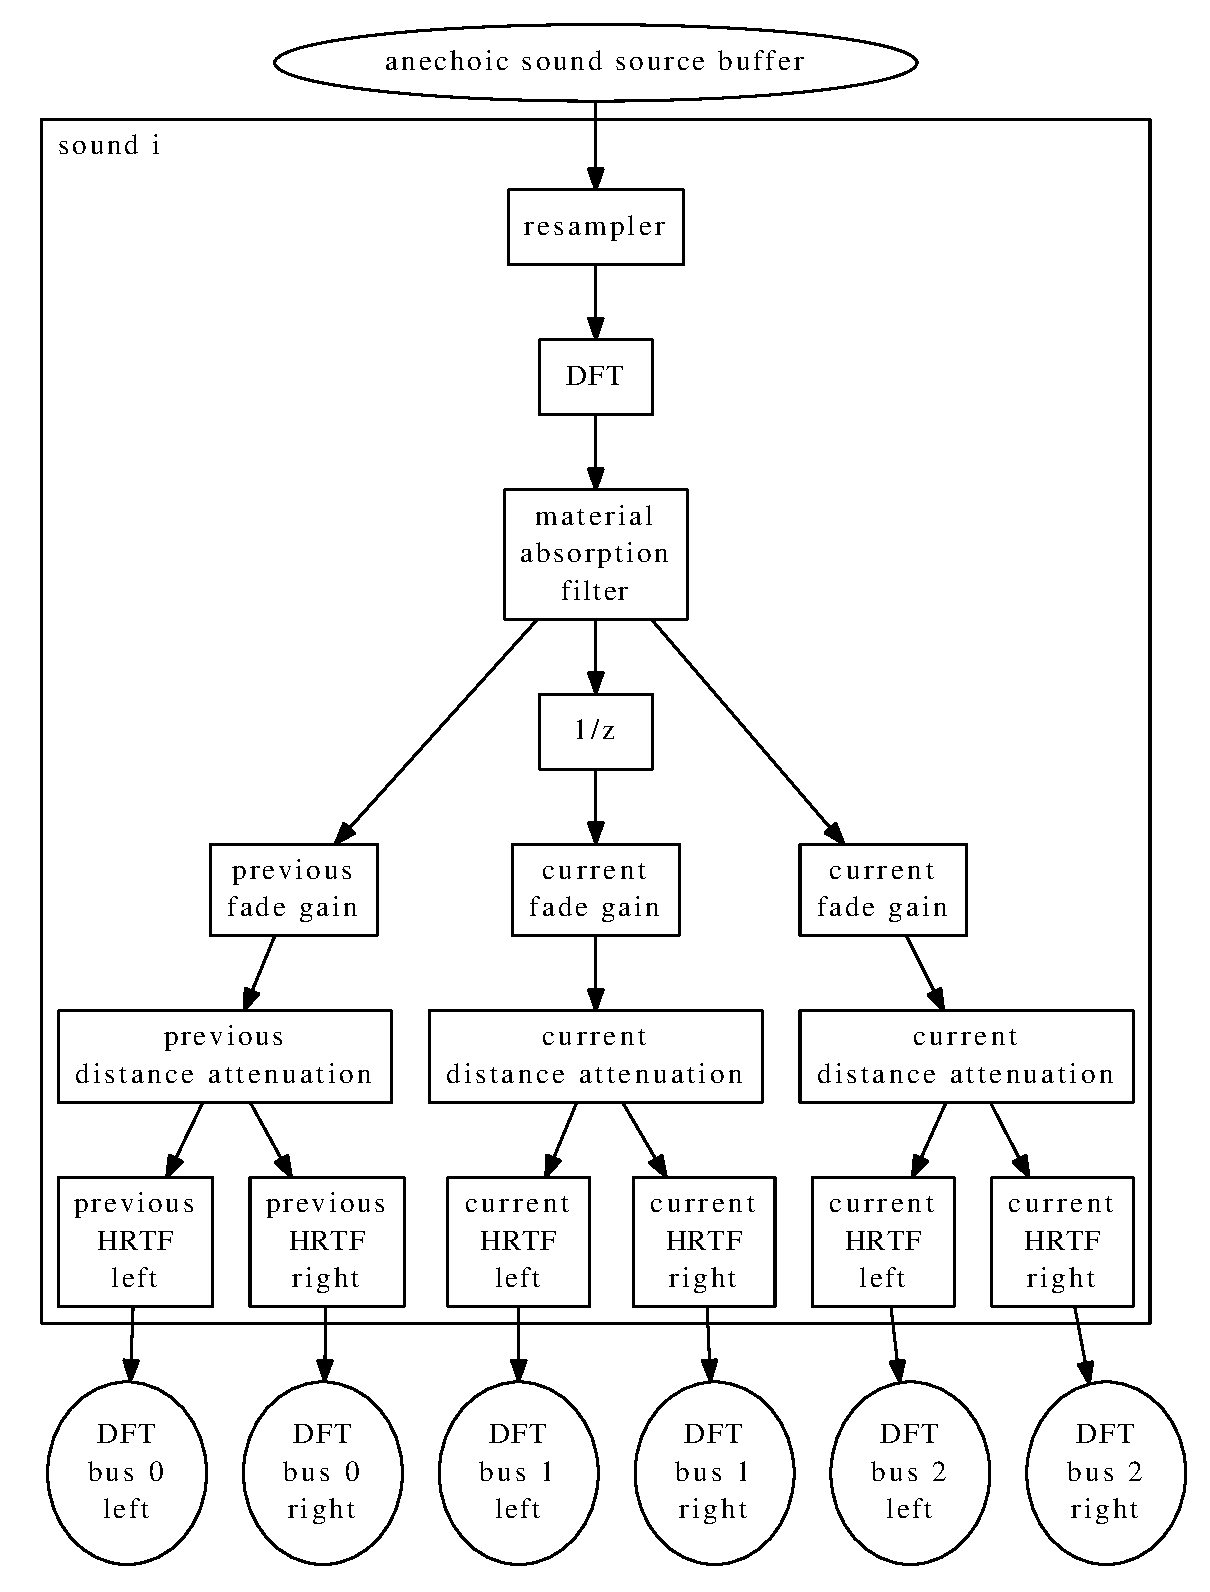
\includegraphics[width=\textwidth]{audio3}
\caption{Individual sound processing block diagram}
\end{DoxyImage}


The anechoic sound source buffer is a ring buffer that contains the anechoic audio data of the sound source, supplied by \hyperlink{aave_8h_a546bf3fff8b9009ddc744a6908154f5e}{aave\-\_\-put\-\_\-audio()}. Each sound originated from this sound source gets its input audio data from this ring buffer, from the delayed audio sample position corresponding to the travelled distance of that particular sound.

When the listener or sound sources move, the travelled distances change, in a discontinuous manner, since the positions' update rate is usually much lower than the audio sampling rate. The resampler block is responsible for producing a stream of audio data without discontinuities, from the discontinuous distance values. It does this by upsampling and low-\/pass filtering the distance values, and then interpolating (zero-\/order) the audio samples in the ring buffer with the corresponding fractional delay, as described in\-: Peter Brinkman and Michael Gogins, \char`\"{}\-Doppler effects without equations\char`\"{}, Proc. of the 16th Int. Conf. on Digital Audio Effects (D\-A\-Fx-\/13).

The H\-R\-T\-F processing is performed in the frequency domain, using the fast convolution method mentioned in\-: Udo Zolzer, \char`\"{}\-Digital Audio Signal
\-Processing\char`\"{}, 2nd Edition, Section 5.\-3 Nonrecursive Audio Filters. The D\-F\-T block thus zero-\/pads and converts the audio data from time domain to frequency domain, in \hyperlink{dft_8h}{dft.\-h}. Note that, without the resampler block, three D\-F\-T blocks would be needed instead of just one.

The material absorption filter block implements the sound attenuation by frequency band of the materials of the surfaces where the sound reflects. This filtering is efficiently performed in the frequency domain simply by calculating N complex multiplications, in \hyperlink{audio_8c_a5949cca50430419a0d66b75f6bf5793a}{cmul()}. The design of the filter is implemented in \hyperlink{material_8c}{material.\-c}.

The anechoic sound is turned into binaural by applying the H\-R\-T\-F pair that corresponds to the direction (elevation and azimuth) of arrival of the sound relative to the listener's head. When the listener moves her head, the H\-R\-T\-F pair changes. This causes discontinuities in the output binaural sound, mainly due to the phase differences between the previous and current H\-R\-T\-F pair. The greater the movement, the more audible these discontinuities are. To mask these discontinuities, it is implemented a method that applies both H\-R\-T\-F pairs, corresponding to the previous and current directions, and then fades-\/out the previous and fades-\/in the current. It is a multiple-\/sound and binaural version of the algorithm described in\-: Tom Barker et al, \char`\"{}\-Real-\/time auralisation system for virtual microphone
positioning\char`\"{}, Proc. of the 15th Int. Conf. on Digital Audio Effects (D\-A\-Fx12).

The fade-\/in/out gains of appearing/disappearing sounds and the amplitude attenuations of sounds with distance are also performed in the frequency domain, taking advantage that they can be applied at the same time the H\-R\-T\-F filter is, simply by multiplying the magnitude of the frequency response by the appropriate combined gain value, in \hyperlink{audio_8c_a4e6a8bd6af1e6e28fb9f4a59802913d6}{cmadd()}.

The result of each sound processing block is therefore 3 binaural audio signals (6 total), still in the frequency domain\-: D\-F\-T bus 0 with the current anechoic audio block processed with the previous distance and direction parametres, D\-F\-T bus 1 with the previous block processed with the current parametres, and D\-F\-T bus 2 with the current block processed with the current parametres.

The binaural audio signals now need to be converted back to the time domain. But instead of performing 6 inverse discrete Fourier transforms (I\-D\-F\-T) per sound and then summing them in the time domain, the different sounds are summed still in the frequency domain, into the D\-F\-T busses pictured. This way, only 6 I\-D\-F\-T are performed in total, independently of the number of sounds.

To complete the fast convolution method, the sounds in the 6 busses, now in the time domain, are overlap-\/added, as described in\-: Udo Zolzer, \char`\"{}\-Digital Audio Signal Processing\char`\"{}, 2nd Edition, Section 5.\-3.\-2 Fast Convolution of Long Sequences. \begin{DoxyRefDesc}{Todo}
\item[\hyperlink{todo__todo000005}{Todo}]Here, it might be more efficient to use the overlap-\/save method instead of the overlap-\/add method.\end{DoxyRefDesc}


Linear fade-\/outs and fade-\/ins are then applied to the previous and current parametre busses, respectively, to complete the crossfade method described in Tom Barker et al (see above).

At this point, the left and right signals contain the binaural auralisation of the direct sounds and reflection sounds up to a given reflection order. An artificial reverberation tail, implemented in reverb.\-c, is finally added to simulate the late reflections that the \hyperlink{geometry_8c}{geometry.\-c} part could not calculate. 

\subsection{Macro Definition Documentation}
\hypertarget{audio_8c_a7921e52736402cbfff73045ce89695e7}{\index{audio.\-c@{audio.\-c}!A\-A\-V\-E\-\_\-\-D\-I\-S\-T\-A\-N\-C\-E\-\_\-\-B1@{A\-A\-V\-E\-\_\-\-D\-I\-S\-T\-A\-N\-C\-E\-\_\-\-B1}}
\index{A\-A\-V\-E\-\_\-\-D\-I\-S\-T\-A\-N\-C\-E\-\_\-\-B1@{A\-A\-V\-E\-\_\-\-D\-I\-S\-T\-A\-N\-C\-E\-\_\-\-B1}!audio.c@{audio.\-c}}
\subsubsection[{A\-A\-V\-E\-\_\-\-D\-I\-S\-T\-A\-N\-C\-E\-\_\-\-B1}]{\setlength{\rightskip}{0pt plus 5cm}\#define A\-A\-V\-E\-\_\-\-D\-I\-S\-T\-A\-N\-C\-E\-\_\-\-B1~0.\-99977}}\label{audio_8c_a7921e52736402cbfff73045ce89695e7}
The b1 coefficient of the single-\/pole, low-\/pass, recursive filter implemented in the resampler block to smooth the distance values\-:

y\mbox{[}n\mbox{]} = b1 $\ast$ y\mbox{[}n-\/1\mbox{]} + (1 -\/ b1) $\ast$ x\mbox{[}n\mbox{]}

Design steps\-:

d = number of samples for the filter to decay to 36.\-8\%

If the distance is updated at about 10\-Hz (0.\-1s), then we could make\-:

d = 0.\-1 $\ast$ fs = 0.\-1 $\ast$ 44100 = 4410 samples

Then obtain the b1 coefficient\-:

b1 = exp(-\/1/d) = exp(-\/1/4410) $\sim$= 0.\-99977

Reference\-: The Scientist and Engineer's Guide to D\-S\-P, chapter 19. \hypertarget{audio_8c_addce93e897e9f71ef5c263ffd893f831}{\index{audio.\-c@{audio.\-c}!A\-A\-V\-E\-\_\-\-F\-A\-D\-E\-\_\-\-S\-A\-M\-P\-L\-E\-S@{A\-A\-V\-E\-\_\-\-F\-A\-D\-E\-\_\-\-S\-A\-M\-P\-L\-E\-S}}
\index{A\-A\-V\-E\-\_\-\-F\-A\-D\-E\-\_\-\-S\-A\-M\-P\-L\-E\-S@{A\-A\-V\-E\-\_\-\-F\-A\-D\-E\-\_\-\-S\-A\-M\-P\-L\-E\-S}!audio.c@{audio.\-c}}
\subsubsection[{A\-A\-V\-E\-\_\-\-F\-A\-D\-E\-\_\-\-S\-A\-M\-P\-L\-E\-S}]{\setlength{\rightskip}{0pt plus 5cm}\#define A\-A\-V\-E\-\_\-\-F\-A\-D\-E\-\_\-\-S\-A\-M\-P\-L\-E\-S~4096}}\label{audio_8c_addce93e897e9f71ef5c263ffd893f831}
Duration of the fade-\/in/out for appearing/disappering sounds, in number of audio samples (must be a multiple of A\-A\-V\-E\-\_\-\-M\-A\-X\-\_\-\-H\-R\-T\-F)\-: 4096 samples / 44100 Hz $\sim$= 93ms. \hypertarget{audio_8c_a11ddec9c2a797ebe5e6b6f2ae522404f}{\index{audio.\-c@{audio.\-c}!D\-F\-T\-\_\-\-T\-Y\-P\-E@{D\-F\-T\-\_\-\-T\-Y\-P\-E}}
\index{D\-F\-T\-\_\-\-T\-Y\-P\-E@{D\-F\-T\-\_\-\-T\-Y\-P\-E}!audio.c@{audio.\-c}}
\subsubsection[{D\-F\-T\-\_\-\-T\-Y\-P\-E}]{\setlength{\rightskip}{0pt plus 5cm}\#define D\-F\-T\-\_\-\-T\-Y\-P\-E~short}}\label{audio_8c_a11ddec9c2a797ebe5e6b6f2ae522404f}
Create a \hyperlink{dft_8h_ad9584a3bdc946bf6faece23f05dc797d}{dft()} function to convert 16-\/bit audio samples to frequency. \hypertarget{audio_8c_afd47bdf71dbf8a1adbddc63efd267700}{\index{audio.\-c@{audio.\-c}!I\-D\-F\-T\-\_\-\-T\-Y\-P\-E@{I\-D\-F\-T\-\_\-\-T\-Y\-P\-E}}
\index{I\-D\-F\-T\-\_\-\-T\-Y\-P\-E@{I\-D\-F\-T\-\_\-\-T\-Y\-P\-E}!audio.c@{audio.\-c}}
\subsubsection[{I\-D\-F\-T\-\_\-\-T\-Y\-P\-E}]{\setlength{\rightskip}{0pt plus 5cm}\#define I\-D\-F\-T\-\_\-\-T\-Y\-P\-E~int}}\label{audio_8c_afd47bdf71dbf8a1adbddc63efd267700}
Create an \hyperlink{idft_8h_a797484e3f3d53d566ececbcfcd90f537}{idft()} function to convert frequency to 32-\/bit audio samples. 

\subsection{Function Documentation}
\hypertarget{audio_8c_a8dfc247d60dfeb02fe97ae7353731506}{\index{audio.\-c@{audio.\-c}!aave\-\_\-audio\-\_\-source\-\_\-block@{aave\-\_\-audio\-\_\-source\-\_\-block}}
\index{aave\-\_\-audio\-\_\-source\-\_\-block@{aave\-\_\-audio\-\_\-source\-\_\-block}!audio.c@{audio.\-c}}
\subsubsection[{aave\-\_\-audio\-\_\-source\-\_\-block}]{\setlength{\rightskip}{0pt plus 5cm}static void aave\-\_\-audio\-\_\-source\-\_\-block (
\begin{DoxyParamCaption}
\item[{struct {\bf aave\-\_\-sound} $\ast$}]{sound, }
\item[{float}]{distance, }
\item[{short $\ast$}]{x, }
\item[{unsigned}]{frames, }
\item[{unsigned}]{delay}
\end{DoxyParamCaption}
)\hspace{0.3cm}{\ttfamily [static]}}}\label{audio_8c_a8dfc247d60dfeb02fe97ae7353731506}
Generate one audio source block. {\ttfamily sound} is the sound whose source to get the anechoic audio data from, {\ttfamily distance} is the distance from the (image) source to the listener, {\ttfamily x} is the buffer to store the generated audio data, {\ttfamily frames} is the number of frames (anechoic samples) to generate, and {\ttfamily delay} is the number of frames of pre-\/delay to apply to the sound to account for audio user blocks larger than the size of the H\-R\-T\-Fs.

The distance value changes abruptly between audio blocks every time the listener or the sound source move. To generate audio blocks without discontinuities, the anechoic samples of the sound source are resampled, using first-\/order interpolation (linear interpolation), a good compromise between audio quality and processing time, to match an upsampled and low-\/ pass filtered version of the discontinuous distance value, as described in Peter Brinkman and Michael Gogins, \char`\"{}\-Doppler effects without equations\char`\"{}, Proc. of the 16th Int. Conf. on Digital Audio Effects (D\-A\-Fx-\/13). 

Here is the call graph for this function\-:\nopagebreak
\begin{figure}[H]
\begin{center}
\leavevmode
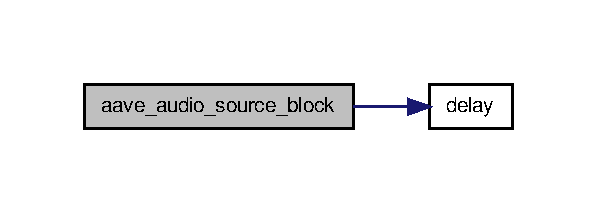
\includegraphics[width=286pt]{audio_8c_a8dfc247d60dfeb02fe97ae7353731506_cgraph}
\end{center}
\end{figure}




Here is the caller graph for this function\-:\nopagebreak
\begin{figure}[H]
\begin{center}
\leavevmode
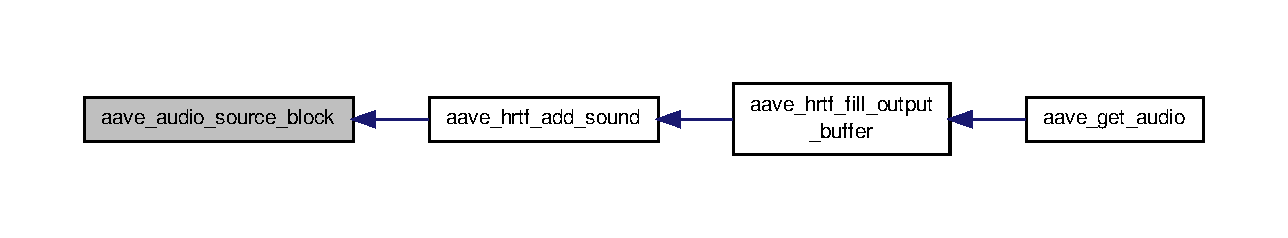
\includegraphics[width=350pt]{audio_8c_a8dfc247d60dfeb02fe97ae7353731506_icgraph}
\end{center}
\end{figure}


\hypertarget{audio_8c_afe43a0d12af335e2f133c0da2a99422f}{\index{audio.\-c@{audio.\-c}!aave\-\_\-get\-\_\-audio@{aave\-\_\-get\-\_\-audio}}
\index{aave\-\_\-get\-\_\-audio@{aave\-\_\-get\-\_\-audio}!audio.c@{audio.\-c}}
\subsubsection[{aave\-\_\-get\-\_\-audio}]{\setlength{\rightskip}{0pt plus 5cm}void aave\-\_\-get\-\_\-audio (
\begin{DoxyParamCaption}
\item[{struct {\bf aave} $\ast$}]{aave, }
\item[{short $\ast$}]{buf, }
\item[{unsigned}]{n}
\end{DoxyParamCaption}
)}}\label{audio_8c_afe43a0d12af335e2f133c0da2a99422f}
Generate {\ttfamily n} 16-\/bit 2-\/channel frames of the auralisation world {\ttfamily aave} and put them in the memory location pointed by {\ttfamily buf}. 

Here is the call graph for this function\-:\nopagebreak
\begin{figure}[H]
\begin{center}
\leavevmode
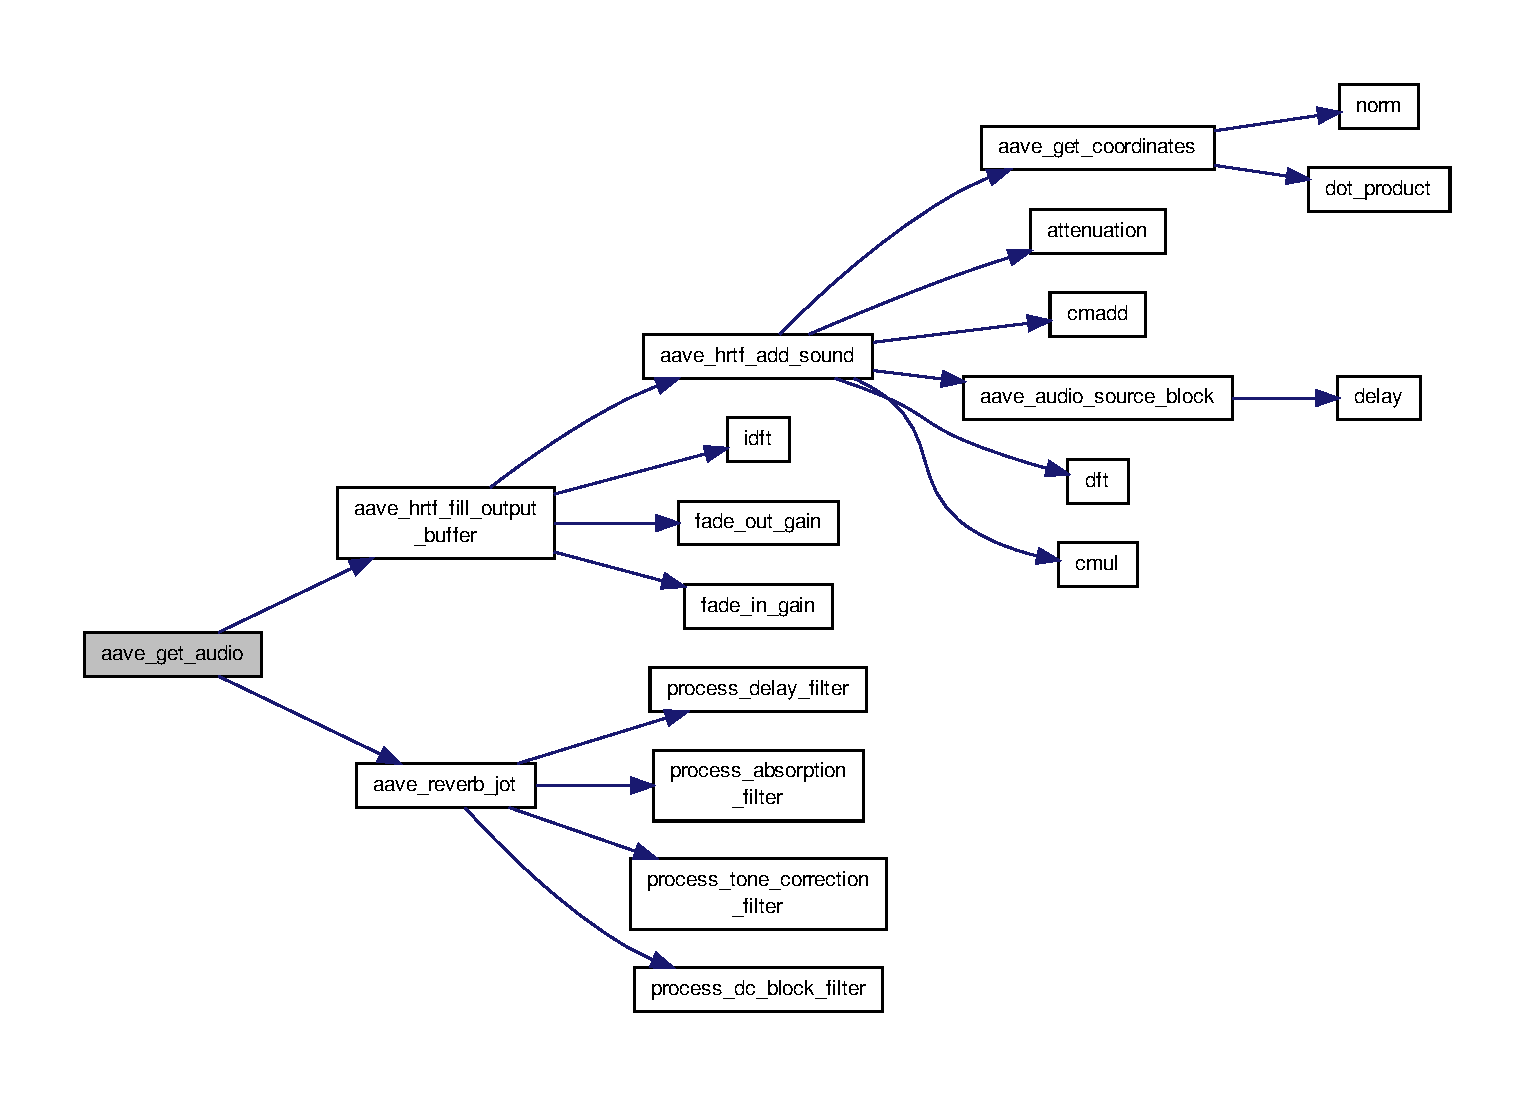
\includegraphics[width=350pt]{audio_8c_afe43a0d12af335e2f133c0da2a99422f_cgraph}
\end{center}
\end{figure}


\hypertarget{audio_8c_a74e68044085a9e60e9d9065100a520b0}{\index{audio.\-c@{audio.\-c}!aave\-\_\-hrtf\-\_\-add\-\_\-sound@{aave\-\_\-hrtf\-\_\-add\-\_\-sound}}
\index{aave\-\_\-hrtf\-\_\-add\-\_\-sound@{aave\-\_\-hrtf\-\_\-add\-\_\-sound}!audio.c@{audio.\-c}}
\subsubsection[{aave\-\_\-hrtf\-\_\-add\-\_\-sound}]{\setlength{\rightskip}{0pt plus 5cm}static void aave\-\_\-hrtf\-\_\-add\-\_\-sound (
\begin{DoxyParamCaption}
\item[{struct {\bf aave} $\ast$}]{aave, }
\item[{struct {\bf aave\-\_\-sound} $\ast$}]{sound, }
\item[{float}]{ydft\mbox{[}3\mbox{]}\mbox{[}2\mbox{]}\mbox{[}\-A\-A\-V\-E\-\_\-\-M\-A\-X\-\_\-\-H\-R\-T\-F $\ast$4\mbox{]}, }
\item[{unsigned}]{delay, }
\item[{unsigned}]{frames}
\end{DoxyParamCaption}
)\hspace{0.3cm}{\ttfamily [static]}}}\label{audio_8c_a74e68044085a9e60e9d9065100a520b0}
Process one {\ttfamily sound} and add it to the D\-F\-T busses {\ttfamily ydft}. {\ttfamily frames} is the number of frames to process. {\ttfamily delay} is the number of frames of pre-\/delay to apply to the sound to account for audio user blocks larger than the size of the H\-R\-T\-Fs. 

Here is the call graph for this function\-:\nopagebreak
\begin{figure}[H]
\begin{center}
\leavevmode
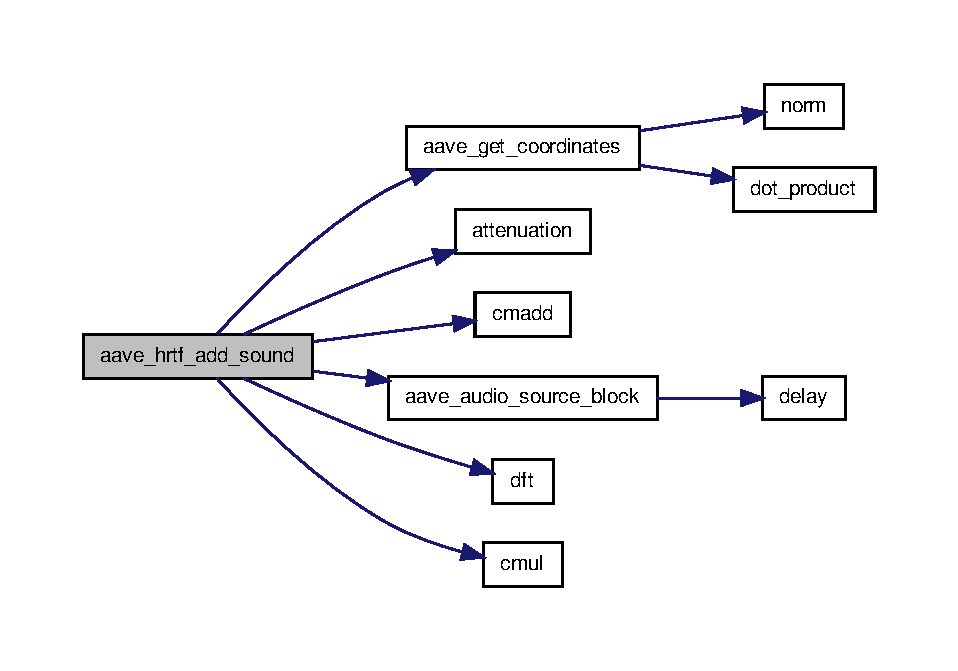
\includegraphics[width=350pt]{audio_8c_a74e68044085a9e60e9d9065100a520b0_cgraph}
\end{center}
\end{figure}




Here is the caller graph for this function\-:\nopagebreak
\begin{figure}[H]
\begin{center}
\leavevmode
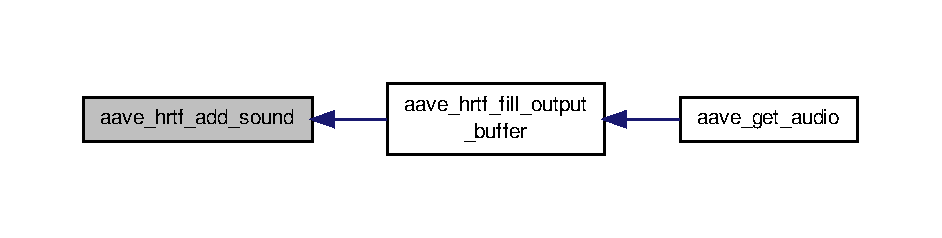
\includegraphics[width=350pt]{audio_8c_a74e68044085a9e60e9d9065100a520b0_icgraph}
\end{center}
\end{figure}


\hypertarget{audio_8c_a0435bc74e8d5edca85e72ab93a72bc37}{\index{audio.\-c@{audio.\-c}!aave\-\_\-hrtf\-\_\-fill\-\_\-output\-\_\-buffer@{aave\-\_\-hrtf\-\_\-fill\-\_\-output\-\_\-buffer}}
\index{aave\-\_\-hrtf\-\_\-fill\-\_\-output\-\_\-buffer@{aave\-\_\-hrtf\-\_\-fill\-\_\-output\-\_\-buffer}!audio.c@{audio.\-c}}
\subsubsection[{aave\-\_\-hrtf\-\_\-fill\-\_\-output\-\_\-buffer}]{\setlength{\rightskip}{0pt plus 5cm}static void aave\-\_\-hrtf\-\_\-fill\-\_\-output\-\_\-buffer (
\begin{DoxyParamCaption}
\item[{struct {\bf aave} $\ast$}]{aave, }
\item[{unsigned}]{delay, }
\item[{unsigned}]{frames}
\end{DoxyParamCaption}
)\hspace{0.3cm}{\ttfamily [static]}}}\label{audio_8c_a0435bc74e8d5edca85e72ab93a72bc37}
Generate one audio buffer of binaural data for the auralisation world {\ttfamily aave} with all sounds in it. {\ttfamily frames} is the number of frames to generate. {\ttfamily delay} is the number of frames of pre-\/delay to apply to all sounds to account for audio user blocks larger than the size of the H\-R\-T\-Fs. 

Here is the call graph for this function\-:\nopagebreak
\begin{figure}[H]
\begin{center}
\leavevmode
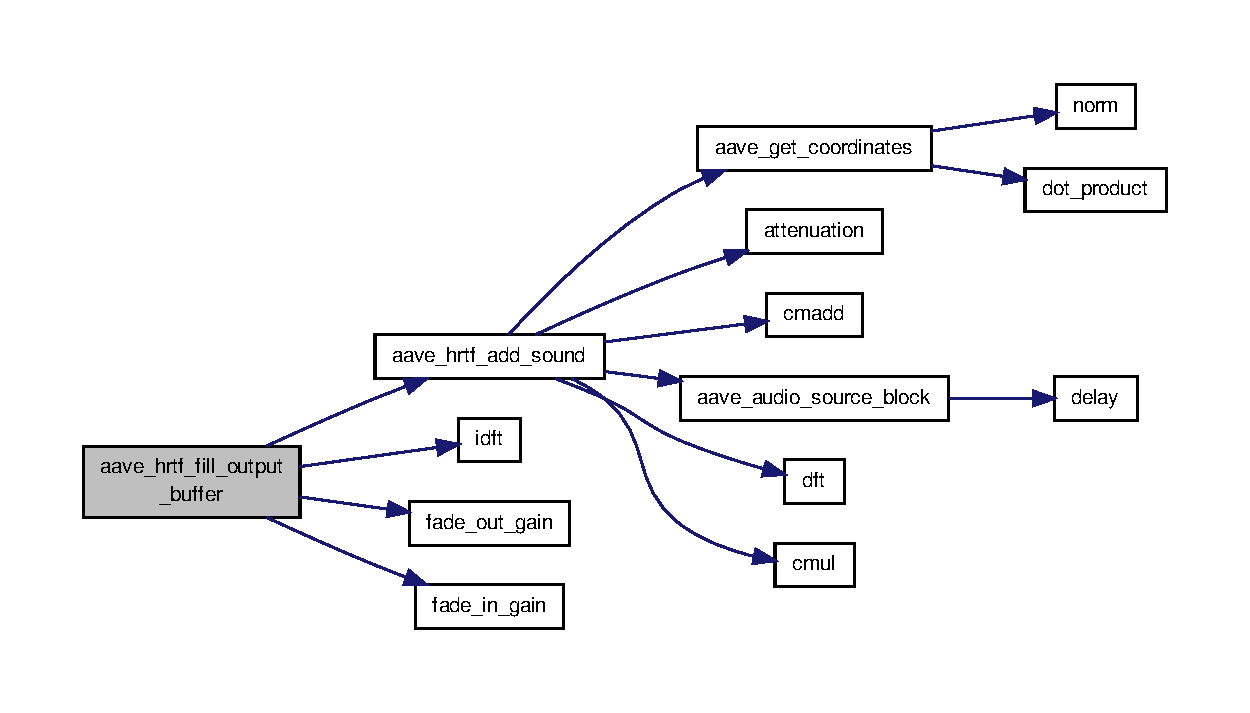
\includegraphics[width=350pt]{audio_8c_a0435bc74e8d5edca85e72ab93a72bc37_cgraph}
\end{center}
\end{figure}




Here is the caller graph for this function\-:\nopagebreak
\begin{figure}[H]
\begin{center}
\leavevmode
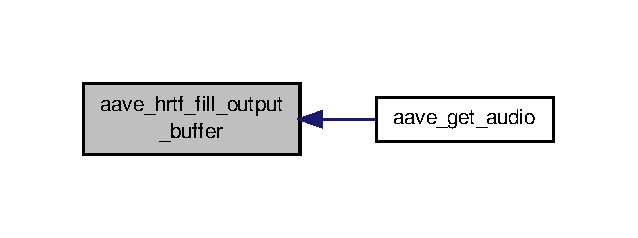
\includegraphics[width=306pt]{audio_8c_a0435bc74e8d5edca85e72ab93a72bc37_icgraph}
\end{center}
\end{figure}


\hypertarget{audio_8c_a8652f21a39abdea73f6ad975ad7af5fd}{\index{audio.\-c@{audio.\-c}!aave\-\_\-put\-\_\-audio@{aave\-\_\-put\-\_\-audio}}
\index{aave\-\_\-put\-\_\-audio@{aave\-\_\-put\-\_\-audio}!audio.c@{audio.\-c}}
\subsubsection[{aave\-\_\-put\-\_\-audio}]{\setlength{\rightskip}{0pt plus 5cm}void aave\-\_\-put\-\_\-audio (
\begin{DoxyParamCaption}
\item[{struct {\bf aave\-\_\-source} $\ast$}]{source, }
\item[{const short $\ast$}]{audio, }
\item[{unsigned}]{n}
\end{DoxyParamCaption}
)}}\label{audio_8c_a8652f21a39abdea73f6ad975ad7af5fd}
Put the {\ttfamily n} frames pointed by {\ttfamily audio} in the ring buffer of {\ttfamily source}. \hypertarget{audio_8c_a01cdef4fc35ac0cf58e59bed7c2af7d9}{\index{audio.\-c@{audio.\-c}!attenuation@{attenuation}}
\index{attenuation@{attenuation}!audio.c@{audio.\-c}}
\subsubsection[{attenuation}]{\setlength{\rightskip}{0pt plus 5cm}static float attenuation (
\begin{DoxyParamCaption}
\item[{float}]{distance}
\end{DoxyParamCaption}
)\hspace{0.3cm}{\ttfamily [static]}}}\label{audio_8c_a01cdef4fc35ac0cf58e59bed7c2af7d9}
Return the gain corresponding to the amplitude attenuation of a sound at the specified {\ttfamily distance} (m). 

Here is the caller graph for this function\-:\nopagebreak
\begin{figure}[H]
\begin{center}
\leavevmode
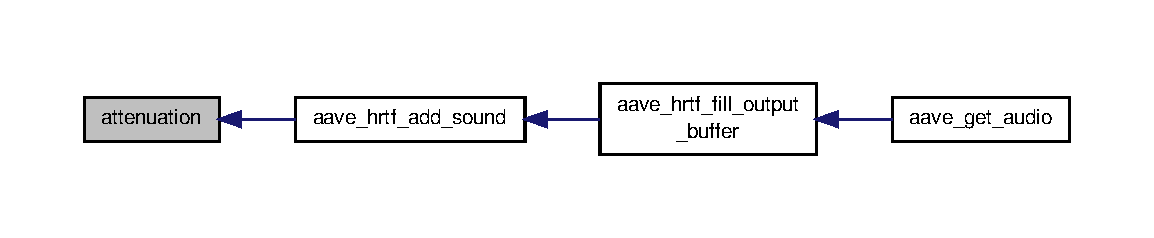
\includegraphics[width=350pt]{audio_8c_a01cdef4fc35ac0cf58e59bed7c2af7d9_icgraph}
\end{center}
\end{figure}


\hypertarget{audio_8c_a4e6a8bd6af1e6e28fb9f4a59802913d6}{\index{audio.\-c@{audio.\-c}!cmadd@{cmadd}}
\index{cmadd@{cmadd}!audio.c@{audio.\-c}}
\subsubsection[{cmadd}]{\setlength{\rightskip}{0pt plus 5cm}static void cmadd (
\begin{DoxyParamCaption}
\item[{float $\ast$}]{y, }
\item[{const float $\ast$}]{a, }
\item[{const float $\ast$}]{b, }
\item[{unsigned}]{n, }
\item[{float}]{g}
\end{DoxyParamCaption}
)\hspace{0.3cm}{\ttfamily [static]}}}\label{audio_8c_a4e6a8bd6af1e6e28fb9f4a59802913d6}
Calculate the Complex Multiplication and A\-D\-Dition {\ttfamily y} += {\ttfamily g} $\ast$ {\ttfamily a} $\ast$ {\ttfamily b} of size {\ttfamily n}.

Y += g $\ast$ A $\ast$ B

Y += g $\ast$ (ar + j ai) $\ast$ (br + j br)

Y += g $\ast$ (ar $\ast$ br -\/ ai $\ast$ bi) + j g $\ast$ (ar $\ast$ bi + ai $\ast$ br) 

Here is the caller graph for this function\-:\nopagebreak
\begin{figure}[H]
\begin{center}
\leavevmode
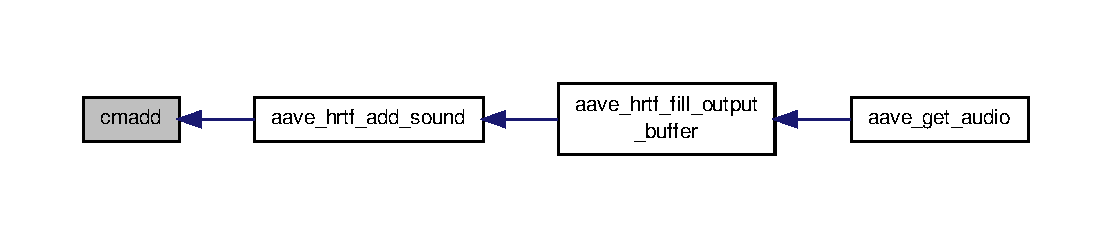
\includegraphics[width=350pt]{audio_8c_a4e6a8bd6af1e6e28fb9f4a59802913d6_icgraph}
\end{center}
\end{figure}


\hypertarget{audio_8c_a5949cca50430419a0d66b75f6bf5793a}{\index{audio.\-c@{audio.\-c}!cmul@{cmul}}
\index{cmul@{cmul}!audio.c@{audio.\-c}}
\subsubsection[{cmul}]{\setlength{\rightskip}{0pt plus 5cm}static void cmul (
\begin{DoxyParamCaption}
\item[{float $\ast$}]{a, }
\item[{const float $\ast$}]{b, }
\item[{unsigned}]{n}
\end{DoxyParamCaption}
)\hspace{0.3cm}{\ttfamily [static]}}}\label{audio_8c_a5949cca50430419a0d66b75f6bf5793a}
Calculate the Complex M\-U\-Ltiplication {\ttfamily a} = {\ttfamily a} $\ast$ {\ttfamily b} of size {\ttfamily n}.

A = A $\ast$ B

A = (ar + j ai) $\ast$ (br + j br)

A = (ar $\ast$ br -\/ ai $\ast$ bi) + j (ar $\ast$ bi + ai $\ast$ br) 

Here is the caller graph for this function\-:\nopagebreak
\begin{figure}[H]
\begin{center}
\leavevmode
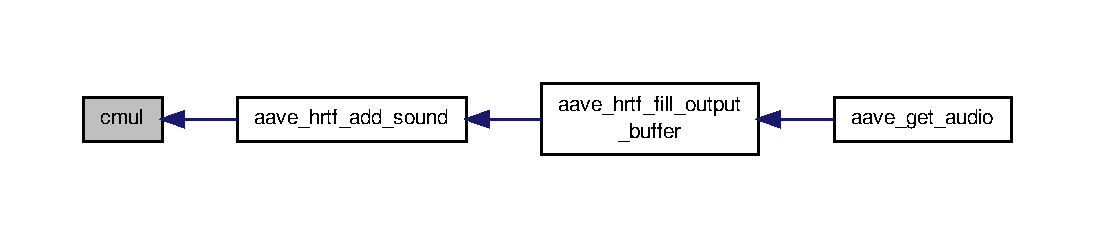
\includegraphics[width=350pt]{audio_8c_a5949cca50430419a0d66b75f6bf5793a_icgraph}
\end{center}
\end{figure}


\hypertarget{audio_8c_a0ed45f17383de6ca52241b5ac60a10b2}{\index{audio.\-c@{audio.\-c}!fade\-\_\-in\-\_\-gain@{fade\-\_\-in\-\_\-gain}}
\index{fade\-\_\-in\-\_\-gain@{fade\-\_\-in\-\_\-gain}!audio.c@{audio.\-c}}
\subsubsection[{fade\-\_\-in\-\_\-gain}]{\setlength{\rightskip}{0pt plus 5cm}static float fade\-\_\-in\-\_\-gain (
\begin{DoxyParamCaption}
\item[{unsigned}]{i, }
\item[{unsigned}]{frames}
\end{DoxyParamCaption}
)\hspace{0.3cm}{\ttfamily [static]}}}\label{audio_8c_a0ed45f17383de6ca52241b5ac60a10b2}
Return the fade-\/in gain at index {\ttfamily i} for a window of the specified {\ttfamily frames}. 

Here is the caller graph for this function\-:\nopagebreak
\begin{figure}[H]
\begin{center}
\leavevmode
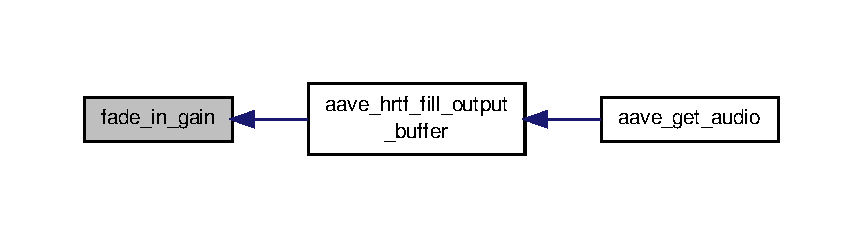
\includegraphics[width=350pt]{audio_8c_a0ed45f17383de6ca52241b5ac60a10b2_icgraph}
\end{center}
\end{figure}


\hypertarget{audio_8c_a3bff6ddd40eda3065aa82561d23e51a6}{\index{audio.\-c@{audio.\-c}!fade\-\_\-out\-\_\-gain@{fade\-\_\-out\-\_\-gain}}
\index{fade\-\_\-out\-\_\-gain@{fade\-\_\-out\-\_\-gain}!audio.c@{audio.\-c}}
\subsubsection[{fade\-\_\-out\-\_\-gain}]{\setlength{\rightskip}{0pt plus 5cm}static float fade\-\_\-out\-\_\-gain (
\begin{DoxyParamCaption}
\item[{unsigned}]{i, }
\item[{unsigned}]{frames}
\end{DoxyParamCaption}
)\hspace{0.3cm}{\ttfamily [static]}}}\label{audio_8c_a3bff6ddd40eda3065aa82561d23e51a6}
Return the fade-\/out gain at index {\ttfamily i} for a window of the specified {\ttfamily frames}. 

Here is the caller graph for this function\-:\nopagebreak
\begin{figure}[H]
\begin{center}
\leavevmode
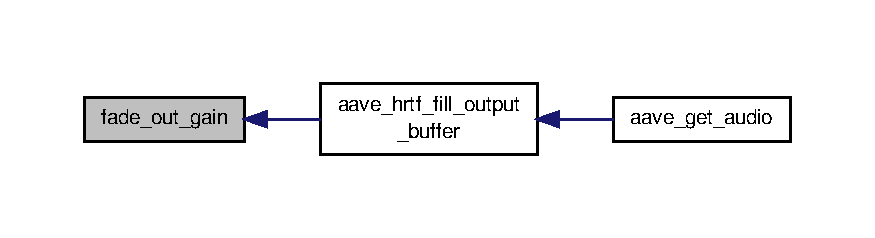
\includegraphics[width=350pt]{audio_8c_a3bff6ddd40eda3065aa82561d23e51a6_icgraph}
\end{center}
\end{figure}



\hypertarget{dft_8h}{\section{dft.\-h File Reference}
\label{dft_8h}\index{dft.\-h@{dft.\-h}}
}
This graph shows which files directly or indirectly include this file\-:\nopagebreak
\begin{figure}[H]
\begin{center}
\leavevmode
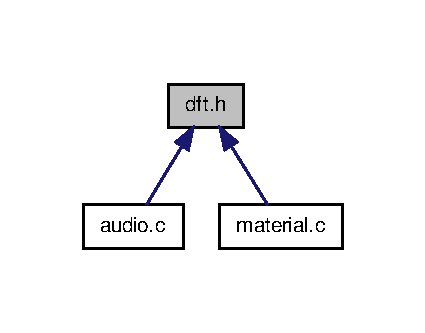
\includegraphics[width=204pt]{dft_8h__dep__incl}
\end{center}
\end{figure}
\subsection*{Functions}
\begin{DoxyCompactItemize}
\item 
static void \hyperlink{dft_8h_ad9584a3bdc946bf6faece23f05dc797d}{dft} (float $\ast$X, const \hyperlink{material_8c_a11ddec9c2a797ebe5e6b6f2ae522404f}{D\-F\-T\-\_\-\-T\-Y\-P\-E} $\ast$x, unsigned n)
\end{DoxyCompactItemize}
\subsection*{Variables}
\begin{DoxyCompactItemize}
\item 
const float \hyperlink{dft_8h_a3196640d8e9b871f615b6a42a6b77123}{dftsincos} \mbox{[}$\,$\mbox{]}\mbox{[}2\mbox{]}
\end{DoxyCompactItemize}


\subsection{Detailed Description}
The \hyperlink{dft_8h}{dft.\-h} file implements the discrete Fourier transform (D\-F\-T) of real-\/input data of power-\/of-\/2 sizes, using the Cooley-\/\-Tukey F\-F\-T algorithm (\href{http://en.wikipedia.org/wiki/Cooley%E2%80%93Tukey_FFT_algorithm}{\tt http\-://en.\-wikipedia.\-org/wiki/\-Cooley\%\-E2\%80\%93\-Tukey\-\_\-\-F\-F\-T\-\_\-algorithm}).

It is about 3 times faster than the equivalent real input to complex-\/\-Hermitian output plan fftw\-\_\-plan\-\_\-dft\-\_\-r2c\-\_\-1d of the fftw library (\href{http://www.fftw.org/}{\tt http\-://www.\-fftw.\-org/}). Furthermore, it implicitly type-\/converts and zero-\/pads the input data to twice the size, making the comparison even more favorable for this implementation.

The drawback is that the ouput Fourier coefficients end up unordered. However, this is irrevelant for our main purpose of performing fast convolutions, because the corresponding inverse discrete Fourier transform (I\-D\-F\-T) implemented in \hyperlink{idft_8h}{idft.\-h} also uses the same order. For the case where it is necessary to know the order of the Fourier coefficients, namely the design of the material absorption filters in \hyperlink{material_8c}{material.\-c}, the function \hyperlink{aave_8h_a5b453c8df5597105b3a7cde336e83e0e}{dft\-\_\-index()} can be used to retrieve the Fourier coefficients in any desired order.

This \hyperlink{dft_8h}{dft.\-h} file is implemented as a \char`\"{}template\char`\"{}. To create a \hyperlink{dft_8h_ad9584a3bdc946bf6faece23f05dc797d}{dft()} function to use in your source code to transform input data of some type, for example type short (16-\/bit audio samples), include the following in your source code file\-: 
\begin{DoxyCode}
\textcolor{preprocessor}{#define DFT\_TYPE short}
\textcolor{preprocessor}{#include "dft.h"}
\end{DoxyCode}
 This will insert a static \hyperlink{dft_8h_ad9584a3bdc946bf6faece23f05dc797d}{dft()} function in your source code file that calculates the Fourier coefficients of an array of short integers. 

\subsection{Function Documentation}
\hypertarget{dft_8h_ad9584a3bdc946bf6faece23f05dc797d}{\index{dft.\-h@{dft.\-h}!dft@{dft}}
\index{dft@{dft}!dft.h@{dft.\-h}}
\subsubsection[{dft}]{\setlength{\rightskip}{0pt plus 5cm}static void dft (
\begin{DoxyParamCaption}
\item[{float $\ast$}]{X, }
\item[{const {\bf D\-F\-T\-\_\-\-T\-Y\-P\-E} $\ast$}]{x, }
\item[{unsigned}]{n}
\end{DoxyParamCaption}
)\hspace{0.3cm}{\ttfamily [static]}}}\label{dft_8h_ad9584a3bdc946bf6faece23f05dc797d}
This dft function calculates the {\ttfamily n} point discrete Fourier transform of the zero-\/padded real-\/input data values pointed by {\ttfamily x} and stores the Fourier coefficients in {\ttfamily X}. {\ttfamily x} points to {\ttfamily n} / 2 elements (elements {\ttfamily n} / 2 to {\ttfamily n} -\/ 1 are implicitly zero-\/padded). {\ttfamily X} points to {\ttfamily n} elements, which correspond to the Fourier coefficients 0 to {\ttfamily n} / 2, (un)ordered as follows\-:
\begin{DoxyItemize}
\item X\mbox{[}0\mbox{]} = X\mbox{[}0\mbox{]}.real;
\item X\mbox{[}1\mbox{]} = X\mbox{[}N/2\mbox{]}.real;
\item X\mbox{[}2\mbox{]} = X\mbox{[}N/4\mbox{]}.real;
\item X\mbox{[}3\mbox{]} = X\mbox{[}N/4\mbox{]}.imag;
\item etc... (see \hyperlink{aave_8h_a5b453c8df5597105b3a7cde336e83e0e}{dft\-\_\-index()} for the complete ordering)
\end{DoxyItemize}

Remember that when the input data is real\-:
\begin{DoxyItemize}
\item X\mbox{[}0\mbox{]}.imag = 0;
\item X\mbox{[}N/2\mbox{]}.imag = 0;
\item X\mbox{[}N/2+i\mbox{]}.real = X\mbox{[}N/2-\/i\mbox{]}.real;
\item X\mbox{[}N/2+i\mbox{]}.imag = -\/ X\mbox{[}N/2-\/i\mbox{]}.imag; 
\end{DoxyItemize}

Here is the caller graph for this function\-:\nopagebreak
\begin{figure}[H]
\begin{center}
\leavevmode
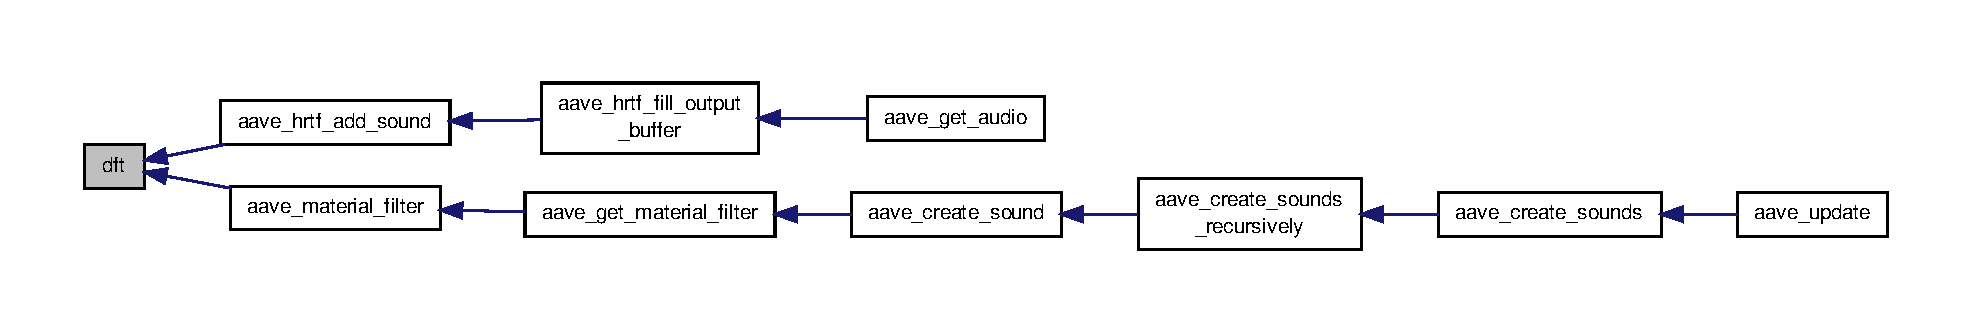
\includegraphics[width=350pt]{dft_8h_ad9584a3bdc946bf6faece23f05dc797d_icgraph}
\end{center}
\end{figure}




\subsection{Variable Documentation}
\hypertarget{dft_8h_a3196640d8e9b871f615b6a42a6b77123}{\index{dft.\-h@{dft.\-h}!dftsincos@{dftsincos}}
\index{dftsincos@{dftsincos}!dft.h@{dft.\-h}}
\subsubsection[{dftsincos}]{\setlength{\rightskip}{0pt plus 5cm}const float dftsincos\mbox{[}$\,$\mbox{]}\mbox{[}2\mbox{]}}}\label{dft_8h_a3196640d8e9b871f615b6a42a6b77123}
Table with the pre-\/calculated sin() and cos() values. 
\hypertarget{dftindex_8c}{\section{dftindex.\-c File Reference}
\label{dftindex_8c}\index{dftindex.\-c@{dftindex.\-c}}
}
\subsection*{Functions}
\begin{DoxyCompactItemize}
\item 
unsigned \hyperlink{dftindex_8c_a5e34ce91dceab1bfa22527c9fbba970b}{dft\-\_\-index} (unsigned i, unsigned n)
\end{DoxyCompactItemize}
\subsection*{Variables}
\begin{DoxyCompactItemize}
\item 
static const unsigned char \hyperlink{dftindex_8c_ad9fc4c6b2778357224f5341cf268f78c}{dft\-\_\-index\-\_\-table} \mbox{[}$\,$\mbox{]}
\end{DoxyCompactItemize}


\subsection{Detailed Description}
The discrete Fourier transform (D\-F\-T) implementation in \hyperlink{dft_8h}{dft.\-h} stores the Fourier coefficients in non-\/sequential order. This \hyperlink{dftindex_8c}{dftindex.\-c} file implements a \hyperlink{aave_8h_a5b453c8df5597105b3a7cde336e83e0e}{dft\-\_\-index()} function that returns the index into the calculated D\-F\-T data that corresponds to each Fourier coefficient. 

\subsection{Function Documentation}
\hypertarget{dftindex_8c_a5e34ce91dceab1bfa22527c9fbba970b}{\index{dftindex.\-c@{dftindex.\-c}!dft\-\_\-index@{dft\-\_\-index}}
\index{dft\-\_\-index@{dft\-\_\-index}!dftindex.c@{dftindex.\-c}}
\subsubsection[{dft\-\_\-index}]{\setlength{\rightskip}{0pt plus 5cm}unsigned dft\-\_\-index (
\begin{DoxyParamCaption}
\item[{unsigned}]{i, }
\item[{unsigned}]{n}
\end{DoxyParamCaption}
)}}\label{dftindex_8c_a5e34ce91dceab1bfa22527c9fbba970b}
This function returns the index into the D\-F\-T data calculated by \hyperlink{dft_8h_ad9584a3bdc946bf6faece23f05dc797d}{dft()} that contains the Fourier coefficient {\ttfamily i} for a D\-F\-T of size {\ttfamily n}. {\ttfamily n} is a power of 2, up to the maximum supported by dft\-\_\-index\-\_\-table (currently 128). {\ttfamily i} is a value from 0 up to {\ttfamily n} / 2 -\/ 1, since the input data is real\-:
\begin{DoxyItemize}
\item X\mbox{[}0\mbox{]} = X\mbox{[}0\mbox{]}.real; X\mbox{[}0\mbox{]}.imag = 0;
\item X\mbox{[}1\mbox{]} = X\mbox{[}N/2\mbox{]}.real; X\mbox{[}N/2\mbox{]}.imag = 0;
\item X\mbox{[}N/2+i\mbox{]}.real = X\mbox{[}N/2-\/i\mbox{]}.real;
\item X\mbox{[}N/2+i\mbox{]}.imag = -\/ X\mbox{[}N/2-\/i\mbox{]}.imag; 
\end{DoxyItemize}

Here is the caller graph for this function\-:\nopagebreak
\begin{figure}[H]
\begin{center}
\leavevmode
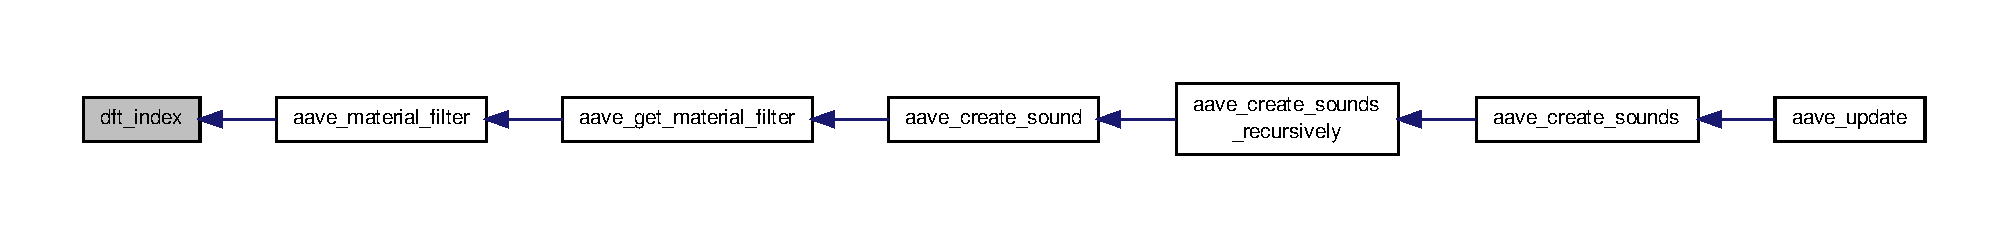
\includegraphics[width=350pt]{dftindex_8c_a5e34ce91dceab1bfa22527c9fbba970b_icgraph}
\end{center}
\end{figure}




\subsection{Variable Documentation}
\hypertarget{dftindex_8c_ad9fc4c6b2778357224f5341cf268f78c}{\index{dftindex.\-c@{dftindex.\-c}!dft\-\_\-index\-\_\-table@{dft\-\_\-index\-\_\-table}}
\index{dft\-\_\-index\-\_\-table@{dft\-\_\-index\-\_\-table}!dftindex.c@{dftindex.\-c}}
\subsubsection[{dft\-\_\-index\-\_\-table}]{\setlength{\rightskip}{0pt plus 5cm}const unsigned char dft\-\_\-index\-\_\-table\mbox{[}$\,$\mbox{]}\hspace{0.3cm}{\ttfamily [static]}}}\label{dftindex_8c_ad9fc4c6b2778357224f5341cf268f78c}
The D\-F\-T index lookup table, for N = 128. This means the \hyperlink{aave_8h_a5b453c8df5597105b3a7cde336e83e0e}{dft\-\_\-index()} function therefore only supports N $<$= 128. \begin{DoxyRefDesc}{Todo}
\item[\hyperlink{todo__todo000006}{Todo}]If the order of the material absorption filter designed in \hyperlink{material_8c}{material.\-c} increases to N $>$ 128, increase this table accordingly. \end{DoxyRefDesc}

\hypertarget{geometry_8c}{\section{geometry.\-c File Reference}
\label{geometry_8c}\index{geometry.\-c@{geometry.\-c}}
}
{\ttfamily \#include $<$math.\-h$>$}\\*
{\ttfamily \#include $<$stdlib.\-h$>$}\\*
{\ttfamily \#include \char`\"{}aave.\-h\char`\"{}}\\*
Include dependency graph for geometry.\-c\-:\nopagebreak
\begin{figure}[H]
\begin{center}
\leavevmode
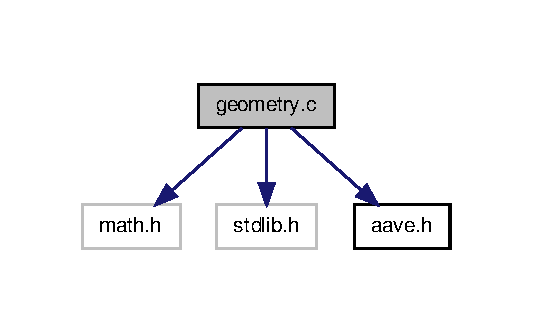
\includegraphics[width=256pt]{geometry_8c__incl}
\end{center}
\end{figure}
\subsection*{Functions}
\begin{DoxyCompactItemize}
\item 
static float \hyperlink{geometry_8c_a373b4381636c15ec96dbc6f3e4655798}{dot\-\_\-product} (const float a\mbox{[}3\mbox{]}, const float b\mbox{[}3\mbox{]})
\item 
static void \hyperlink{geometry_8c_a5e59594bab3bc1ecd8e25ad887a4372f}{cross\-\_\-product} (float n\mbox{[}3\mbox{]}, const float a\mbox{[}3\mbox{]}, const float b\mbox{[}3\mbox{]})
\item 
static float \hyperlink{geometry_8c_adbb79889a33b12c8b090faa854af8109}{norm} (const float x\mbox{[}3\mbox{]})
\item 
static void \hyperlink{geometry_8c_a87c81ecc33ad5301b6c3b1584fc84525}{normalise} (float y\mbox{[}3\mbox{]}, const float x\mbox{[}3\mbox{]})
\item 
static void \hyperlink{geometry_8c_ab40fce8a1525cf5d9194e909227c942d}{aave\-\_\-image\-\_\-source} (const struct \hyperlink{structaave__surface}{aave\-\_\-surface} $\ast$surface, const float source\mbox{[}3\mbox{]}, float image\mbox{[}3\mbox{]})
\item 
static void \hyperlink{geometry_8c_abfbdee9c2e4714938fd9e458f08cbd40}{local\-\_\-coordinates} (float y\mbox{[}2\mbox{]}, const float x\mbox{[}3\mbox{]}, const struct \hyperlink{structaave__surface}{aave\-\_\-surface} $\ast$surface)
\item 
static int \hyperlink{geometry_8c_a4b47f01d4d88d73e92bdcca2d690140a}{aave\-\_\-intersection} (const struct \hyperlink{structaave__surface}{aave\-\_\-surface} $\ast$surface, const float a\mbox{[}3\mbox{]}, const float b\mbox{[}3\mbox{]}, const float v\mbox{[}3\mbox{]}, float xyz\mbox{[}3\mbox{]})
\item 
static int \hyperlink{geometry_8c_a2a9db056c43a4f4b2aece2329a98e2eb}{aave\-\_\-is\-\_\-visible} (const struct \hyperlink{structaave}{aave} $\ast$\hyperlink{structaave}{aave}, const float a\mbox{[}3\mbox{]}, const float b\mbox{[}3\mbox{]})
\item 
static int \hyperlink{geometry_8c_a814ea9c79e9276c9e6407192d3bfb3c1}{aave\-\_\-build\-\_\-sound\-\_\-path} (struct \hyperlink{structaave}{aave} $\ast$\hyperlink{structaave}{aave}, struct \hyperlink{structaave__source}{aave\-\_\-source} $\ast$source, unsigned order, struct \hyperlink{structaave__surface}{aave\-\_\-surface} $\ast$surfaces\mbox{[}$\,$\mbox{]}, float image\-\_\-sources\mbox{[}$\,$\mbox{]}\mbox{[}3\mbox{]}, float x\mbox{[}$\,$\mbox{]}\mbox{[}3\mbox{]})
\item 
static void \hyperlink{geometry_8c_a59ff10a7f9bd39866063bb05918d3df0}{aave\-\_\-create\-\_\-sound} (struct \hyperlink{structaave}{aave} $\ast$\hyperlink{structaave}{aave}, struct \hyperlink{structaave__source}{aave\-\_\-source} $\ast$source, unsigned order, struct \hyperlink{structaave__surface}{aave\-\_\-surface} $\ast$surfaces\mbox{[}$\,$\mbox{]}, float image\-\_\-sources\mbox{[}$\,$\mbox{]}\mbox{[}3\mbox{]})
\item 
static void \hyperlink{geometry_8c_a2c55d6e06ff73570a887d18807442412}{aave\-\_\-create\-\_\-sounds\-\_\-recursively} (struct \hyperlink{structaave}{aave} $\ast$\hyperlink{structaave}{aave}, struct \hyperlink{structaave__source}{aave\-\_\-source} $\ast$source, unsigned order, unsigned o, struct \hyperlink{structaave__surface}{aave\-\_\-surface} $\ast$surfaces\mbox{[}$\,$\mbox{]}, float image\-\_\-sources\mbox{[}$\,$\mbox{]}\mbox{[}3\mbox{]})
\item 
static void \hyperlink{geometry_8c_ab67540c77da19bfc111eaa423d500d33}{aave\-\_\-create\-\_\-sounds} (struct \hyperlink{structaave}{aave} $\ast$\hyperlink{structaave}{aave}, struct \hyperlink{structaave__source}{aave\-\_\-source} $\ast$source, unsigned order)
\item 
static void \hyperlink{geometry_8c_afd54b3e8b06cda8e2f3aaf0e61b61e3b}{aave\-\_\-update\-\_\-sound} (struct \hyperlink{structaave}{aave} $\ast$\hyperlink{structaave}{aave}, struct \hyperlink{structaave__sound}{aave\-\_\-sound} $\ast$sound, unsigned order)
\item 
void \hyperlink{geometry_8c_a8e3a9e9e5e071df68f28a10dd9165ee5}{aave\-\_\-get\-\_\-coordinates} (const struct \hyperlink{structaave}{aave} $\ast$\hyperlink{structaave}{aave}, const float $\ast$source\-\_\-position, float $\ast$distance, float $\ast$elevation, float $\ast$azimuth)
\item 
void \hyperlink{geometry_8c_a2e076058a0c5db597a069c1c83f03f9f}{aave\-\_\-add\-\_\-source} (struct \hyperlink{structaave}{aave} $\ast$\hyperlink{structaave}{aave}, struct \hyperlink{structaave__source}{aave\-\_\-source} $\ast$source)
\item 
void \hyperlink{geometry_8c_a28df3e4ac0fb06ac989de8c42f9f4ab7}{aave\-\_\-add\-\_\-surface} (struct \hyperlink{structaave}{aave} $\ast$\hyperlink{structaave}{aave}, struct \hyperlink{structaave__surface}{aave\-\_\-surface} $\ast$surface)
\item 
void \hyperlink{geometry_8c_a3d6cc2d0548455d9fcd01a8f6057979b}{aave\-\_\-set\-\_\-listener\-\_\-orientation} (struct \hyperlink{structaave}{aave} $\ast$\hyperlink{structaave}{aave}, float roll, float pitch, float yaw)
\item 
void \hyperlink{geometry_8c_a78ea9243574f5e2ae0328e05ce9de845}{aave\-\_\-set\-\_\-listener\-\_\-position} (struct \hyperlink{structaave}{aave} $\ast$\hyperlink{structaave}{aave}, float x, float y, float z)
\item 
void \hyperlink{geometry_8c_a168e1e4d6eb11b303db5272f8a4c22df}{aave\-\_\-set\-\_\-source\-\_\-position} (struct \hyperlink{structaave__source}{aave\-\_\-source} $\ast$source, float x, float y, float z)
\item 
void \hyperlink{geometry_8c_a128fc0893ce9e549392265802bf62d20}{aave\-\_\-update} (struct \hyperlink{structaave}{aave} $\ast$\hyperlink{structaave}{aave})
\end{DoxyCompactItemize}


\subsection{Detailed Description}
The \hyperlink{geometry_8c}{geometry.\-c} file contains the functions that implement the geometry part of the auralisation process, based on the image source model shown in\-: \char`\"{}\-Auralization\-: Fundamentals of Acoustics, Modelling, Simulation,
\-Algorithms and Acoustic Virtual Reality\char`\"{}, Michael Vorlander, 2008, Section 11.\-3 Image source model.

At startup, the \hyperlink{aave_8h_a20e98109bd38d422444f2959c0a6b80c}{aave\-\_\-add\-\_\-surface()} function is called for each surface, and the \hyperlink{aave_8h_af609d22b339f6a53d988e4c73f4b7dfb}{aave\-\_\-add\-\_\-source()} function is called for each sound source, to build the auralisation world.

At runtime, the \hyperlink{aave_8h_a41a4224263cd8432d79099871d542b2e}{aave\-\_\-set\-\_\-listener\-\_\-position()} or \hyperlink{aave_8h_ad48ffc19be78794acb7bf0f9a6397c11}{aave\-\_\-set\-\_\-source\-\_\-position()} functions are called when the listener or sound sources move, followed by \hyperlink{aave_8h_a5acfa7c6e7e714ff364cda9dabd7a2f8}{aave\-\_\-update()} to perform all geometric calculations to discover the audible sounds for the new positions, and the \hyperlink{aave_8h_aee300969973298dab868f91f7b94724d}{aave\-\_\-set\-\_\-listener\-\_\-orientation()} function is called when the listener moves her head. 

\subsection{Function Documentation}
\hypertarget{geometry_8c_a2e076058a0c5db597a069c1c83f03f9f}{\index{geometry.\-c@{geometry.\-c}!aave\-\_\-add\-\_\-source@{aave\-\_\-add\-\_\-source}}
\index{aave\-\_\-add\-\_\-source@{aave\-\_\-add\-\_\-source}!geometry.c@{geometry.\-c}}
\subsubsection[{aave\-\_\-add\-\_\-source}]{\setlength{\rightskip}{0pt plus 5cm}void aave\-\_\-add\-\_\-source (
\begin{DoxyParamCaption}
\item[{struct {\bf aave} $\ast$}]{aave, }
\item[{struct {\bf aave\-\_\-source} $\ast$}]{source}
\end{DoxyParamCaption}
)}}\label{geometry_8c_a2e076058a0c5db597a069c1c83f03f9f}
Add a sound source to the auralisation world. \hypertarget{geometry_8c_a28df3e4ac0fb06ac989de8c42f9f4ab7}{\index{geometry.\-c@{geometry.\-c}!aave\-\_\-add\-\_\-surface@{aave\-\_\-add\-\_\-surface}}
\index{aave\-\_\-add\-\_\-surface@{aave\-\_\-add\-\_\-surface}!geometry.c@{geometry.\-c}}
\subsubsection[{aave\-\_\-add\-\_\-surface}]{\setlength{\rightskip}{0pt plus 5cm}void aave\-\_\-add\-\_\-surface (
\begin{DoxyParamCaption}
\item[{struct {\bf aave} $\ast$}]{aave, }
\item[{struct {\bf aave\-\_\-surface} $\ast$}]{surface}
\end{DoxyParamCaption}
)}}\label{geometry_8c_a28df3e4ac0fb06ac989de8c42f9f4ab7}
Add a surface to the auralisation world. 

Here is the call graph for this function\-:\nopagebreak
\begin{figure}[H]
\begin{center}
\leavevmode
\includegraphics[width=350pt]{geometry_8c_a28df3e4ac0fb06ac989de8c42f9f4ab7_cgraph}
\end{center}
\end{figure}




Here is the caller graph for this function\-:\nopagebreak
\begin{figure}[H]
\begin{center}
\leavevmode
\includegraphics[width=292pt]{geometry_8c_a28df3e4ac0fb06ac989de8c42f9f4ab7_icgraph}
\end{center}
\end{figure}


\hypertarget{geometry_8c_a814ea9c79e9276c9e6407192d3bfb3c1}{\index{geometry.\-c@{geometry.\-c}!aave\-\_\-build\-\_\-sound\-\_\-path@{aave\-\_\-build\-\_\-sound\-\_\-path}}
\index{aave\-\_\-build\-\_\-sound\-\_\-path@{aave\-\_\-build\-\_\-sound\-\_\-path}!geometry.c@{geometry.\-c}}
\subsubsection[{aave\-\_\-build\-\_\-sound\-\_\-path}]{\setlength{\rightskip}{0pt plus 5cm}static int aave\-\_\-build\-\_\-sound\-\_\-path (
\begin{DoxyParamCaption}
\item[{struct {\bf aave} $\ast$}]{aave, }
\item[{struct {\bf aave\-\_\-source} $\ast$}]{source, }
\item[{unsigned}]{order, }
\item[{struct {\bf aave\-\_\-surface} $\ast$}]{surfaces\mbox{[}$\,$\mbox{]}, }
\item[{float}]{image\-\_\-sources\mbox{[}$\,$\mbox{]}\mbox{[}3\mbox{]}, }
\item[{float}]{x\mbox{[}$\,$\mbox{]}\mbox{[}3\mbox{]}}
\end{DoxyParamCaption}
)\hspace{0.3cm}{\ttfamily [static]}}}\label{geometry_8c_a814ea9c79e9276c9e6407192d3bfb3c1}
Create the sound path from the source pointed by  to the listerner, for reflection order {\ttfamily order}, that reflects on the specified sequence of {\ttfamily surfaces}, with corresponding image source positions {\ttfamily image\-\_\-sources}. The calculated reflection points are stored in {\ttfamily x}. Returns 1 if the sound path is audible, or 0 otherwise. 

Here is the call graph for this function\-:\nopagebreak
\begin{figure}[H]
\begin{center}
\leavevmode
\includegraphics[width=350pt]{geometry_8c_a814ea9c79e9276c9e6407192d3bfb3c1_cgraph}
\end{center}
\end{figure}




Here is the caller graph for this function\-:\nopagebreak
\begin{figure}[H]
\begin{center}
\leavevmode
\includegraphics[width=350pt]{geometry_8c_a814ea9c79e9276c9e6407192d3bfb3c1_icgraph}
\end{center}
\end{figure}


\hypertarget{geometry_8c_a59ff10a7f9bd39866063bb05918d3df0}{\index{geometry.\-c@{geometry.\-c}!aave\-\_\-create\-\_\-sound@{aave\-\_\-create\-\_\-sound}}
\index{aave\-\_\-create\-\_\-sound@{aave\-\_\-create\-\_\-sound}!geometry.c@{geometry.\-c}}
\subsubsection[{aave\-\_\-create\-\_\-sound}]{\setlength{\rightskip}{0pt plus 5cm}static void aave\-\_\-create\-\_\-sound (
\begin{DoxyParamCaption}
\item[{struct {\bf aave} $\ast$}]{aave, }
\item[{struct {\bf aave\-\_\-source} $\ast$}]{source, }
\item[{unsigned}]{order, }
\item[{struct {\bf aave\-\_\-surface} $\ast$}]{surfaces\mbox{[}$\,$\mbox{]}, }
\item[{float}]{image\-\_\-sources\mbox{[}$\,$\mbox{]}\mbox{[}3\mbox{]}}
\end{DoxyParamCaption}
)\hspace{0.3cm}{\ttfamily [static]}}}\label{geometry_8c_a59ff10a7f9bd39866063bb05918d3df0}
Create a sound to be auralised by the audio processing. {\ttfamily source} is the sound source that originates the sound, {\ttfamily order} is the reflection order of the sound, {\ttfamily surfaces} is the sequence of surfaces where the sound reflects, and {\ttfamily image\-\_\-sources} are the positions of the corresponding image-\/sources. 

Here is the call graph for this function\-:\nopagebreak
\begin{figure}[H]
\begin{center}
\leavevmode
\includegraphics[width=350pt]{geometry_8c_a59ff10a7f9bd39866063bb05918d3df0_cgraph}
\end{center}
\end{figure}




Here is the caller graph for this function\-:\nopagebreak
\begin{figure}[H]
\begin{center}
\leavevmode
\includegraphics[width=350pt]{geometry_8c_a59ff10a7f9bd39866063bb05918d3df0_icgraph}
\end{center}
\end{figure}


\hypertarget{geometry_8c_ab67540c77da19bfc111eaa423d500d33}{\index{geometry.\-c@{geometry.\-c}!aave\-\_\-create\-\_\-sounds@{aave\-\_\-create\-\_\-sounds}}
\index{aave\-\_\-create\-\_\-sounds@{aave\-\_\-create\-\_\-sounds}!geometry.c@{geometry.\-c}}
\subsubsection[{aave\-\_\-create\-\_\-sounds}]{\setlength{\rightskip}{0pt plus 5cm}static void aave\-\_\-create\-\_\-sounds (
\begin{DoxyParamCaption}
\item[{struct {\bf aave} $\ast$}]{aave, }
\item[{struct {\bf aave\-\_\-source} $\ast$}]{source, }
\item[{unsigned}]{order}
\end{DoxyParamCaption}
)\hspace{0.3cm}{\ttfamily [static]}}}\label{geometry_8c_ab67540c77da19bfc111eaa423d500d33}
Create all audible sounds originated from the specified sound source up to, and including, the specified reflection order. 

Here is the call graph for this function\-:\nopagebreak
\begin{figure}[H]
\begin{center}
\leavevmode
\includegraphics[width=350pt]{geometry_8c_ab67540c77da19bfc111eaa423d500d33_cgraph}
\end{center}
\end{figure}




Here is the caller graph for this function\-:\nopagebreak
\begin{figure}[H]
\begin{center}
\leavevmode
\includegraphics[width=296pt]{geometry_8c_ab67540c77da19bfc111eaa423d500d33_icgraph}
\end{center}
\end{figure}


\hypertarget{geometry_8c_a2c55d6e06ff73570a887d18807442412}{\index{geometry.\-c@{geometry.\-c}!aave\-\_\-create\-\_\-sounds\-\_\-recursively@{aave\-\_\-create\-\_\-sounds\-\_\-recursively}}
\index{aave\-\_\-create\-\_\-sounds\-\_\-recursively@{aave\-\_\-create\-\_\-sounds\-\_\-recursively}!geometry.c@{geometry.\-c}}
\subsubsection[{aave\-\_\-create\-\_\-sounds\-\_\-recursively}]{\setlength{\rightskip}{0pt plus 5cm}static void aave\-\_\-create\-\_\-sounds\-\_\-recursively (
\begin{DoxyParamCaption}
\item[{struct {\bf aave} $\ast$}]{aave, }
\item[{struct {\bf aave\-\_\-source} $\ast$}]{source, }
\item[{unsigned}]{order, }
\item[{unsigned}]{o, }
\item[{struct {\bf aave\-\_\-surface} $\ast$}]{surfaces\mbox{[}$\,$\mbox{]}, }
\item[{float}]{image\-\_\-sources\mbox{[}$\,$\mbox{]}\mbox{[}3\mbox{]}}
\end{DoxyParamCaption}
)\hspace{0.3cm}{\ttfamily [static]}}}\label{geometry_8c_a2c55d6e06ff73570a887d18807442412}
Recursively create all audible sounds of a given reflection order that originate from a sound source. {\ttfamily source} is the sound source, {\ttfamily order} is the reflection order, {\ttfamily o} is the current reflection order in the recursive process, {\ttfamily surfaces} is the stack of surfaces where the current sound reflects, {\ttfamily image\-\_\-sources} is the stack of corresponding image source positions.

\begin{DoxyRefDesc}{Todo}
\item[\hyperlink{todo__todo000007}{Todo}]Implement the iterative version of this recursive algorithm. \end{DoxyRefDesc}


Here is the call graph for this function\-:\nopagebreak
\begin{figure}[H]
\begin{center}
\leavevmode
\includegraphics[width=350pt]{geometry_8c_a2c55d6e06ff73570a887d18807442412_cgraph}
\end{center}
\end{figure}




Here is the caller graph for this function\-:\nopagebreak
\begin{figure}[H]
\begin{center}
\leavevmode
\includegraphics[width=350pt]{geometry_8c_a2c55d6e06ff73570a887d18807442412_icgraph}
\end{center}
\end{figure}


\hypertarget{geometry_8c_a8e3a9e9e5e071df68f28a10dd9165ee5}{\index{geometry.\-c@{geometry.\-c}!aave\-\_\-get\-\_\-coordinates@{aave\-\_\-get\-\_\-coordinates}}
\index{aave\-\_\-get\-\_\-coordinates@{aave\-\_\-get\-\_\-coordinates}!geometry.c@{geometry.\-c}}
\subsubsection[{aave\-\_\-get\-\_\-coordinates}]{\setlength{\rightskip}{0pt plus 5cm}void aave\-\_\-get\-\_\-coordinates (
\begin{DoxyParamCaption}
\item[{const struct {\bf aave} $\ast$}]{aave, }
\item[{const float $\ast$}]{source\-\_\-position, }
\item[{float $\ast$}]{distance, }
\item[{float $\ast$}]{elevation, }
\item[{float $\ast$}]{azimuth}
\end{DoxyParamCaption}
)}}\label{geometry_8c_a8e3a9e9e5e071df68f28a10dd9165ee5}
Get the {\ttfamily distance} (m), {\ttfamily azimuth} (rad) and {\ttfamily elevation} (rad) coordinates of the position {\ttfamily source\-\_\-position} of a source relative to the listener. 

Here is the call graph for this function\-:\nopagebreak
\begin{figure}[H]
\begin{center}
\leavevmode
\includegraphics[width=296pt]{geometry_8c_a8e3a9e9e5e071df68f28a10dd9165ee5_cgraph}
\end{center}
\end{figure}




Here is the caller graph for this function\-:\nopagebreak
\begin{figure}[H]
\begin{center}
\leavevmode
\includegraphics[width=350pt]{geometry_8c_a8e3a9e9e5e071df68f28a10dd9165ee5_icgraph}
\end{center}
\end{figure}


\hypertarget{geometry_8c_ab40fce8a1525cf5d9194e909227c942d}{\index{geometry.\-c@{geometry.\-c}!aave\-\_\-image\-\_\-source@{aave\-\_\-image\-\_\-source}}
\index{aave\-\_\-image\-\_\-source@{aave\-\_\-image\-\_\-source}!geometry.c@{geometry.\-c}}
\subsubsection[{aave\-\_\-image\-\_\-source}]{\setlength{\rightskip}{0pt plus 5cm}static void aave\-\_\-image\-\_\-source (
\begin{DoxyParamCaption}
\item[{const struct {\bf aave\-\_\-surface} $\ast$}]{surface, }
\item[{const float}]{source\mbox{[}3\mbox{]}, }
\item[{float}]{image\mbox{[}3\mbox{]}}
\end{DoxyParamCaption}
)\hspace{0.3cm}{\ttfamily [static]}}}\label{geometry_8c_ab40fce8a1525cf5d9194e909227c942d}
Calculate the position \mbox{[}x,y,z\mbox{]} of the image-\/source of the sound source at position {\ttfamily source} created by the surface pointed by {\ttfamily surface}. The position of the image-\/source is returned in {\ttfamily image}.

Reference\-: \char`\"{}\-Auralization\-: Fundamentals of Acoustics, Modelling,
\-Simulation, Algorithms and Acoustic Virtual Reality\char`\"{}, Michael Vorlander, 2008, Section 11.\-3.\-1 Classical model. 

Here is the call graph for this function\-:\nopagebreak
\begin{figure}[H]
\begin{center}
\leavevmode
\includegraphics[width=288pt]{geometry_8c_ab40fce8a1525cf5d9194e909227c942d_cgraph}
\end{center}
\end{figure}




Here is the caller graph for this function\-:\nopagebreak
\begin{figure}[H]
\begin{center}
\leavevmode
\includegraphics[width=350pt]{geometry_8c_ab40fce8a1525cf5d9194e909227c942d_icgraph}
\end{center}
\end{figure}


\hypertarget{geometry_8c_a4b47f01d4d88d73e92bdcca2d690140a}{\index{geometry.\-c@{geometry.\-c}!aave\-\_\-intersection@{aave\-\_\-intersection}}
\index{aave\-\_\-intersection@{aave\-\_\-intersection}!geometry.c@{geometry.\-c}}
\subsubsection[{aave\-\_\-intersection}]{\setlength{\rightskip}{0pt plus 5cm}static int aave\-\_\-intersection (
\begin{DoxyParamCaption}
\item[{const struct {\bf aave\-\_\-surface} $\ast$}]{surface, }
\item[{const float}]{a\mbox{[}3\mbox{]}, }
\item[{const float}]{b\mbox{[}3\mbox{]}, }
\item[{const float}]{v\mbox{[}3\mbox{]}, }
\item[{float}]{xyz\mbox{[}3\mbox{]}}
\end{DoxyParamCaption}
)\hspace{0.3cm}{\ttfamily [static]}}}\label{geometry_8c_a4b47f01d4d88d73e92bdcca2d690140a}
Check if the vector {\ttfamily v} (a line segment from point {\ttfamily a} to point {\ttfamily b}) intersects the surface pointed by {\ttfamily surface}. Returns 0 if false or 1 if true, and the intersection point in {\ttfamily xyz}.

Reference\-: P\-N\-P\-O\-L\-Y -\/ Point Inclusion in Polygon Test, W. Randolph Franklin, \href{http://www.ecse.rpi.edu/~wrf/Research/Short_Notes/pnpoly.html}{\tt http\-://www.\-ecse.\-rpi.\-edu/$\sim$wrf/\-Research/\-Short\-\_\-\-Notes/pnpoly.\-html} 

Here is the call graph for this function\-:\nopagebreak
\begin{figure}[H]
\begin{center}
\leavevmode
\includegraphics[width=350pt]{geometry_8c_a4b47f01d4d88d73e92bdcca2d690140a_cgraph}
\end{center}
\end{figure}




Here is the caller graph for this function\-:\nopagebreak
\begin{figure}[H]
\begin{center}
\leavevmode
\includegraphics[width=350pt]{geometry_8c_a4b47f01d4d88d73e92bdcca2d690140a_icgraph}
\end{center}
\end{figure}


\hypertarget{geometry_8c_a2a9db056c43a4f4b2aece2329a98e2eb}{\index{geometry.\-c@{geometry.\-c}!aave\-\_\-is\-\_\-visible@{aave\-\_\-is\-\_\-visible}}
\index{aave\-\_\-is\-\_\-visible@{aave\-\_\-is\-\_\-visible}!geometry.c@{geometry.\-c}}
\subsubsection[{aave\-\_\-is\-\_\-visible}]{\setlength{\rightskip}{0pt plus 5cm}static int aave\-\_\-is\-\_\-visible (
\begin{DoxyParamCaption}
\item[{const struct {\bf aave} $\ast$}]{aave, }
\item[{const float}]{a\mbox{[}3\mbox{]}, }
\item[{const float}]{b\mbox{[}3\mbox{]}}
\end{DoxyParamCaption}
)\hspace{0.3cm}{\ttfamily [static]}}}\label{geometry_8c_a2a9db056c43a4f4b2aece2329a98e2eb}
Check if the sound path from point {\ttfamily a} to point {\ttfamily b} is visible. Returns 0 if the line segment b-\/a is intersected by any surface, or 1 otherwise. 

Here is the call graph for this function\-:\nopagebreak
\begin{figure}[H]
\begin{center}
\leavevmode
\includegraphics[width=350pt]{geometry_8c_a2a9db056c43a4f4b2aece2329a98e2eb_cgraph}
\end{center}
\end{figure}




Here is the caller graph for this function\-:\nopagebreak
\begin{figure}[H]
\begin{center}
\leavevmode
\includegraphics[width=350pt]{geometry_8c_a2a9db056c43a4f4b2aece2329a98e2eb_icgraph}
\end{center}
\end{figure}


\hypertarget{geometry_8c_a3d6cc2d0548455d9fcd01a8f6057979b}{\index{geometry.\-c@{geometry.\-c}!aave\-\_\-set\-\_\-listener\-\_\-orientation@{aave\-\_\-set\-\_\-listener\-\_\-orientation}}
\index{aave\-\_\-set\-\_\-listener\-\_\-orientation@{aave\-\_\-set\-\_\-listener\-\_\-orientation}!geometry.c@{geometry.\-c}}
\subsubsection[{aave\-\_\-set\-\_\-listener\-\_\-orientation}]{\setlength{\rightskip}{0pt plus 5cm}void aave\-\_\-set\-\_\-listener\-\_\-orientation (
\begin{DoxyParamCaption}
\item[{struct {\bf aave} $\ast$}]{aave, }
\item[{float}]{roll, }
\item[{float}]{pitch, }
\item[{float}]{yaw}
\end{DoxyParamCaption}
)}}\label{geometry_8c_a3d6cc2d0548455d9fcd01a8f6057979b}
Set the orientation of the listener's head. \hypertarget{geometry_8c_a78ea9243574f5e2ae0328e05ce9de845}{\index{geometry.\-c@{geometry.\-c}!aave\-\_\-set\-\_\-listener\-\_\-position@{aave\-\_\-set\-\_\-listener\-\_\-position}}
\index{aave\-\_\-set\-\_\-listener\-\_\-position@{aave\-\_\-set\-\_\-listener\-\_\-position}!geometry.c@{geometry.\-c}}
\subsubsection[{aave\-\_\-set\-\_\-listener\-\_\-position}]{\setlength{\rightskip}{0pt plus 5cm}void aave\-\_\-set\-\_\-listener\-\_\-position (
\begin{DoxyParamCaption}
\item[{struct {\bf aave} $\ast$}]{aave, }
\item[{float}]{x, }
\item[{float}]{y, }
\item[{float}]{z}
\end{DoxyParamCaption}
)}}\label{geometry_8c_a78ea9243574f5e2ae0328e05ce9de845}
Set the position of the listener.

The \hyperlink{aave_8h_a5acfa7c6e7e714ff364cda9dabd7a2f8}{aave\-\_\-update()} function should be called afterwards to update the state of the auralisation engine to reflect the new position. \hypertarget{geometry_8c_a168e1e4d6eb11b303db5272f8a4c22df}{\index{geometry.\-c@{geometry.\-c}!aave\-\_\-set\-\_\-source\-\_\-position@{aave\-\_\-set\-\_\-source\-\_\-position}}
\index{aave\-\_\-set\-\_\-source\-\_\-position@{aave\-\_\-set\-\_\-source\-\_\-position}!geometry.c@{geometry.\-c}}
\subsubsection[{aave\-\_\-set\-\_\-source\-\_\-position}]{\setlength{\rightskip}{0pt plus 5cm}void aave\-\_\-set\-\_\-source\-\_\-position (
\begin{DoxyParamCaption}
\item[{struct {\bf aave\-\_\-source} $\ast$}]{source, }
\item[{float}]{x, }
\item[{float}]{y, }
\item[{float}]{z}
\end{DoxyParamCaption}
)}}\label{geometry_8c_a168e1e4d6eb11b303db5272f8a4c22df}
Set the position of a sound source.

The \hyperlink{aave_8h_a5acfa7c6e7e714ff364cda9dabd7a2f8}{aave\-\_\-update()} function should be called afterwards to update the state of the auralisation engine to reflect the new position. \hypertarget{geometry_8c_a128fc0893ce9e549392265802bf62d20}{\index{geometry.\-c@{geometry.\-c}!aave\-\_\-update@{aave\-\_\-update}}
\index{aave\-\_\-update@{aave\-\_\-update}!geometry.c@{geometry.\-c}}
\subsubsection[{aave\-\_\-update}]{\setlength{\rightskip}{0pt plus 5cm}void aave\-\_\-update (
\begin{DoxyParamCaption}
\item[{struct {\bf aave} $\ast$}]{aave}
\end{DoxyParamCaption}
)}}\label{geometry_8c_a128fc0893ce9e549392265802bf62d20}
Update the whole state of the auralisation world. Runs the visibility checks for all sounds from all sources. 

Here is the call graph for this function\-:\nopagebreak
\begin{figure}[H]
\begin{center}
\leavevmode
\includegraphics[width=350pt]{geometry_8c_a128fc0893ce9e549392265802bf62d20_cgraph}
\end{center}
\end{figure}


\hypertarget{geometry_8c_afd54b3e8b06cda8e2f3aaf0e61b61e3b}{\index{geometry.\-c@{geometry.\-c}!aave\-\_\-update\-\_\-sound@{aave\-\_\-update\-\_\-sound}}
\index{aave\-\_\-update\-\_\-sound@{aave\-\_\-update\-\_\-sound}!geometry.c@{geometry.\-c}}
\subsubsection[{aave\-\_\-update\-\_\-sound}]{\setlength{\rightskip}{0pt plus 5cm}static void aave\-\_\-update\-\_\-sound (
\begin{DoxyParamCaption}
\item[{struct {\bf aave} $\ast$}]{aave, }
\item[{struct {\bf aave\-\_\-sound} $\ast$}]{sound, }
\item[{unsigned}]{order}
\end{DoxyParamCaption}
)\hspace{0.3cm}{\ttfamily [static]}}}\label{geometry_8c_afd54b3e8b06cda8e2f3aaf0e61b61e3b}
Update the distance and azimuth of the listener relative to a sound source. Calculate the (distance, elevation, azimuth) vector from the listener-\/to-\/source vector (x, y, z) with listener orientation (roll, pitch, yaw). Angles in radians. 

Here is the call graph for this function\-:\nopagebreak
\begin{figure}[H]
\begin{center}
\leavevmode
\includegraphics[width=350pt]{geometry_8c_afd54b3e8b06cda8e2f3aaf0e61b61e3b_cgraph}
\end{center}
\end{figure}




Here is the caller graph for this function\-:\nopagebreak
\begin{figure}[H]
\begin{center}
\leavevmode
\includegraphics[width=292pt]{geometry_8c_afd54b3e8b06cda8e2f3aaf0e61b61e3b_icgraph}
\end{center}
\end{figure}


\hypertarget{geometry_8c_a5e59594bab3bc1ecd8e25ad887a4372f}{\index{geometry.\-c@{geometry.\-c}!cross\-\_\-product@{cross\-\_\-product}}
\index{cross\-\_\-product@{cross\-\_\-product}!geometry.c@{geometry.\-c}}
\subsubsection[{cross\-\_\-product}]{\setlength{\rightskip}{0pt plus 5cm}static void cross\-\_\-product (
\begin{DoxyParamCaption}
\item[{float}]{n\mbox{[}3\mbox{]}, }
\item[{const float}]{a\mbox{[}3\mbox{]}, }
\item[{const float}]{b\mbox{[}3\mbox{]}}
\end{DoxyParamCaption}
)\hspace{0.3cm}{\ttfamily [static]}}}\label{geometry_8c_a5e59594bab3bc1ecd8e25ad887a4372f}
Calculate the cross product n = a x b. 

Here is the caller graph for this function\-:\nopagebreak
\begin{figure}[H]
\begin{center}
\leavevmode
\includegraphics[width=350pt]{geometry_8c_a5e59594bab3bc1ecd8e25ad887a4372f_icgraph}
\end{center}
\end{figure}


\hypertarget{geometry_8c_a373b4381636c15ec96dbc6f3e4655798}{\index{geometry.\-c@{geometry.\-c}!dot\-\_\-product@{dot\-\_\-product}}
\index{dot\-\_\-product@{dot\-\_\-product}!geometry.c@{geometry.\-c}}
\subsubsection[{dot\-\_\-product}]{\setlength{\rightskip}{0pt plus 5cm}static float dot\-\_\-product (
\begin{DoxyParamCaption}
\item[{const float}]{a\mbox{[}3\mbox{]}, }
\item[{const float}]{b\mbox{[}3\mbox{]}}
\end{DoxyParamCaption}
)\hspace{0.3cm}{\ttfamily [static]}}}\label{geometry_8c_a373b4381636c15ec96dbc6f3e4655798}
Calculate the dot product a . b 

Here is the caller graph for this function\-:\nopagebreak
\begin{figure}[H]
\begin{center}
\leavevmode
\includegraphics[width=350pt]{geometry_8c_a373b4381636c15ec96dbc6f3e4655798_icgraph}
\end{center}
\end{figure}


\hypertarget{geometry_8c_abfbdee9c2e4714938fd9e458f08cbd40}{\index{geometry.\-c@{geometry.\-c}!local\-\_\-coordinates@{local\-\_\-coordinates}}
\index{local\-\_\-coordinates@{local\-\_\-coordinates}!geometry.c@{geometry.\-c}}
\subsubsection[{local\-\_\-coordinates}]{\setlength{\rightskip}{0pt plus 5cm}static void local\-\_\-coordinates (
\begin{DoxyParamCaption}
\item[{float}]{y\mbox{[}2\mbox{]}, }
\item[{const float}]{x\mbox{[}3\mbox{]}, }
\item[{const struct {\bf aave\-\_\-surface} $\ast$}]{surface}
\end{DoxyParamCaption}
)\hspace{0.3cm}{\ttfamily [static]}}}\label{geometry_8c_abfbdee9c2e4714938fd9e458f08cbd40}
Calculate the coordinates {\ttfamily y} \mbox{[}x,y\mbox{]} of the point {\ttfamily x} \mbox{[}x,y,z\mbox{]} in the local coordinates of the surface pointed by {\ttfamily surface}. 

Here is the call graph for this function\-:\nopagebreak
\begin{figure}[H]
\begin{center}
\leavevmode
\includegraphics[width=276pt]{geometry_8c_abfbdee9c2e4714938fd9e458f08cbd40_cgraph}
\end{center}
\end{figure}




Here is the caller graph for this function\-:\nopagebreak
\begin{figure}[H]
\begin{center}
\leavevmode
\includegraphics[width=350pt]{geometry_8c_abfbdee9c2e4714938fd9e458f08cbd40_icgraph}
\end{center}
\end{figure}


\hypertarget{geometry_8c_adbb79889a33b12c8b090faa854af8109}{\index{geometry.\-c@{geometry.\-c}!norm@{norm}}
\index{norm@{norm}!geometry.c@{geometry.\-c}}
\subsubsection[{norm}]{\setlength{\rightskip}{0pt plus 5cm}static float norm (
\begin{DoxyParamCaption}
\item[{const float}]{x\mbox{[}3\mbox{]}}
\end{DoxyParamCaption}
)\hspace{0.3cm}{\ttfamily [static]}}}\label{geometry_8c_adbb79889a33b12c8b090faa854af8109}
Calculate the norm of a vector. 

Here is the caller graph for this function\-:\nopagebreak
\begin{figure}[H]
\begin{center}
\leavevmode
\includegraphics[width=350pt]{geometry_8c_adbb79889a33b12c8b090faa854af8109_icgraph}
\end{center}
\end{figure}


\hypertarget{geometry_8c_a87c81ecc33ad5301b6c3b1584fc84525}{\index{geometry.\-c@{geometry.\-c}!normalise@{normalise}}
\index{normalise@{normalise}!geometry.c@{geometry.\-c}}
\subsubsection[{normalise}]{\setlength{\rightskip}{0pt plus 5cm}static void normalise (
\begin{DoxyParamCaption}
\item[{float}]{y\mbox{[}3\mbox{]}, }
\item[{const float}]{x\mbox{[}3\mbox{]}}
\end{DoxyParamCaption}
)\hspace{0.3cm}{\ttfamily [static]}}}\label{geometry_8c_a87c81ecc33ad5301b6c3b1584fc84525}
\char`\"{}\-Normalise\char`\"{} a vector (divide it by its norm)\-: y = x / norm(x) 

Here is the call graph for this function\-:\nopagebreak
\begin{figure}[H]
\begin{center}
\leavevmode
\includegraphics[width=214pt]{geometry_8c_a87c81ecc33ad5301b6c3b1584fc84525_cgraph}
\end{center}
\end{figure}




Here is the caller graph for this function\-:\nopagebreak
\begin{figure}[H]
\begin{center}
\leavevmode
\includegraphics[width=350pt]{geometry_8c_a87c81ecc33ad5301b6c3b1584fc84525_icgraph}
\end{center}
\end{figure}



\hypertarget{hrtf__cipic_8c}{\section{hrtf\-\_\-cipic.\-c File Reference}
\label{hrtf__cipic_8c}\index{hrtf\-\_\-cipic.\-c@{hrtf\-\_\-cipic.\-c}}
}
{\ttfamily \#include \char`\"{}aave.\-h\char`\"{}}\\*
Include dependency graph for hrtf\-\_\-cipic.\-c\-:\nopagebreak
\begin{figure}[H]
\begin{center}
\leavevmode
\includegraphics[width=144pt]{hrtf__cipic_8c__incl}
\end{center}
\end{figure}
\subsection*{Macros}
\begin{DoxyCompactItemize}
\item 
\#define \hyperlink{hrtf__cipic_8c_af2772a1db6305567eacedcc49222733a}{hrtf\-\_\-cipic\-\_\-set}~\hyperlink{hrtf__cipic_8c_ad7826c92f4b287a863202d4ca3243894}{hrtf\-\_\-cipic\-\_\-set\-\_\-008}
\end{DoxyCompactItemize}
\subsection*{Functions}
\begin{DoxyCompactItemize}
\item 
static void \hyperlink{hrtf__cipic_8c_a4b3a15263cf86760cf69027db5aab73a}{aave\-\_\-hrtf\-\_\-cipic\-\_\-get} (const float $\ast$hrtf\mbox{[}2\mbox{]}, int elevation, int azimuth)
\item 
void \hyperlink{hrtf__cipic_8c_a00796d04f8c40370849ef30069d57129}{aave\-\_\-hrtf\-\_\-cipic} (struct \hyperlink{structaave}{aave} $\ast$a)
\end{DoxyCompactItemize}
\subsection*{Variables}
\begin{DoxyCompactItemize}
\item 
const float \hyperlink{hrtf__cipic_8c_ad7826c92f4b287a863202d4ca3243894}{hrtf\-\_\-cipic\-\_\-set\-\_\-008} \mbox{[}$\,$\mbox{]}\mbox{[}1024\mbox{]}
\end{DoxyCompactItemize}


\subsection{Detailed Description}
The \hyperlink{hrtf__cipic_8c}{hrtf\-\_\-cipic.\-c} file implements the interface to use the C\-I\-P\-I\-C H\-R\-T\-F set. To select this set for the auralisation process, call \hyperlink{aave_8h_a9332f29f538c0e54272f61de0e420348}{aave\-\_\-hrtf\-\_\-cipic()} after initialising the aave structure and before calling \hyperlink{aave_8h_a546bf3fff8b9009ddc744a6908154f5e}{aave\-\_\-put\-\_\-audio()}.

The C\-I\-P\-I\-C H\-R\-T\-F set consists of head-\/related impulse responses (H\-R\-I\-R) of 45 subjects. This interface admits using one of them at a time, chosen at compile time.

For each subject, H\-R\-I\-R measurements are available for 64 elevations in 5.\-625 degree steps (360/64) and the following azimuths\-: -\/80, -\/65, -\/55, -\/45 to 45 in 5 degree steps, 55, 65 and 80 degrees. This interface supports all azimuths, but currently only elevation 0.

Each H\-R\-I\-R is 200 samples long at 44100\-Hz ($\sim$4.5ms). Because the discrete Fourier transform (D\-F\-T) implemented in \hyperlink{dft_8h}{dft.\-h} is optimized for powers of 2, each H\-R\-I\-R is zero-\/padded to 256 samples for use in this interface.

References\-: V. R. Algazi, R. O. Duda, D. M. Thompson and C. Avendano, \char`\"{}\-The C\-I\-P\-I\-C H\-R\-T\-F Database\char`\"{}, Proc. 2001 I\-E\-E\-E Workshop on Applications of Signal Processing to Audio and Electroacoustics, pp. 99-\/102, Mohonk Mountain House, New Paltz, N\-Y, Oct. 21-\/24, 2001. 

\subsection{Macro Definition Documentation}
\hypertarget{hrtf__cipic_8c_af2772a1db6305567eacedcc49222733a}{\index{hrtf\-\_\-cipic.\-c@{hrtf\-\_\-cipic.\-c}!hrtf\-\_\-cipic\-\_\-set@{hrtf\-\_\-cipic\-\_\-set}}
\index{hrtf\-\_\-cipic\-\_\-set@{hrtf\-\_\-cipic\-\_\-set}!hrtf_cipic.c@{hrtf\-\_\-cipic.\-c}}
\subsubsection[{hrtf\-\_\-cipic\-\_\-set}]{\setlength{\rightskip}{0pt plus 5cm}\#define hrtf\-\_\-cipic\-\_\-set~{\bf hrtf\-\_\-cipic\-\_\-set\-\_\-008}}}\label{hrtf__cipic_8c_af2772a1db6305567eacedcc49222733a}
The subject of the C\-I\-P\-I\-C H\-R\-T\-F set to use (subject 008). 

\subsection{Function Documentation}
\hypertarget{hrtf__cipic_8c_a00796d04f8c40370849ef30069d57129}{\index{hrtf\-\_\-cipic.\-c@{hrtf\-\_\-cipic.\-c}!aave\-\_\-hrtf\-\_\-cipic@{aave\-\_\-hrtf\-\_\-cipic}}
\index{aave\-\_\-hrtf\-\_\-cipic@{aave\-\_\-hrtf\-\_\-cipic}!hrtf_cipic.c@{hrtf\-\_\-cipic.\-c}}
\subsubsection[{aave\-\_\-hrtf\-\_\-cipic}]{\setlength{\rightskip}{0pt plus 5cm}void aave\-\_\-hrtf\-\_\-cipic (
\begin{DoxyParamCaption}
\item[{struct {\bf aave} $\ast$}]{a}
\end{DoxyParamCaption}
)}}\label{hrtf__cipic_8c_a00796d04f8c40370849ef30069d57129}
Select the C\-I\-P\-I\-C H\-R\-T\-F set for the auralisation process. 

Here is the call graph for this function\-:\nopagebreak
\begin{figure}[H]
\begin{center}
\leavevmode
\includegraphics[width=302pt]{hrtf__cipic_8c_a00796d04f8c40370849ef30069d57129_cgraph}
\end{center}
\end{figure}


\hypertarget{hrtf__cipic_8c_a4b3a15263cf86760cf69027db5aab73a}{\index{hrtf\-\_\-cipic.\-c@{hrtf\-\_\-cipic.\-c}!aave\-\_\-hrtf\-\_\-cipic\-\_\-get@{aave\-\_\-hrtf\-\_\-cipic\-\_\-get}}
\index{aave\-\_\-hrtf\-\_\-cipic\-\_\-get@{aave\-\_\-hrtf\-\_\-cipic\-\_\-get}!hrtf_cipic.c@{hrtf\-\_\-cipic.\-c}}
\subsubsection[{aave\-\_\-hrtf\-\_\-cipic\-\_\-get}]{\setlength{\rightskip}{0pt plus 5cm}static void aave\-\_\-hrtf\-\_\-cipic\-\_\-get (
\begin{DoxyParamCaption}
\item[{const float $\ast$}]{hrtf\mbox{[}2\mbox{]}, }
\item[{int}]{elevation, }
\item[{int}]{azimuth}
\end{DoxyParamCaption}
)\hspace{0.3cm}{\ttfamily [static]}}}\label{hrtf__cipic_8c_a4b3a15263cf86760cf69027db5aab73a}
Get the closest H\-R\-T\-F pair for the specified coordinates. {\ttfamily elevation} is \mbox{[}-\/90;90\mbox{]} degrees. {\ttfamily azimuth} is \mbox{[}-\/180;180\mbox{]} degrees. {\ttfamily hrtf}\mbox{[}0\mbox{]} will be the left H\-R\-T\-F, {\ttfamily hrtf}\mbox{[}1\mbox{]} the right H\-R\-T\-F.

Currently, all elevations map to elevation 0. \begin{DoxyRefDesc}{Todo}
\item[\hyperlink{todo__todo000008}{Todo}]Use all elevation measures available, not just 0 degrees. \end{DoxyRefDesc}


Here is the caller graph for this function\-:\nopagebreak
\begin{figure}[H]
\begin{center}
\leavevmode
\includegraphics[width=302pt]{hrtf__cipic_8c_a4b3a15263cf86760cf69027db5aab73a_icgraph}
\end{center}
\end{figure}




\subsection{Variable Documentation}
\hypertarget{hrtf__cipic_8c_ad7826c92f4b287a863202d4ca3243894}{\index{hrtf\-\_\-cipic.\-c@{hrtf\-\_\-cipic.\-c}!hrtf\-\_\-cipic\-\_\-set\-\_\-008@{hrtf\-\_\-cipic\-\_\-set\-\_\-008}}
\index{hrtf\-\_\-cipic\-\_\-set\-\_\-008@{hrtf\-\_\-cipic\-\_\-set\-\_\-008}!hrtf_cipic.c@{hrtf\-\_\-cipic.\-c}}
\subsubsection[{hrtf\-\_\-cipic\-\_\-set\-\_\-008}]{\setlength{\rightskip}{0pt plus 5cm}const float hrtf\-\_\-cipic\-\_\-set\-\_\-008\mbox{[}$\,$\mbox{]}\mbox{[}1024\mbox{]}}}\label{hrtf__cipic_8c_ad7826c92f4b287a863202d4ca3243894}
The H\-R\-T\-F set, generated by tools/hrtf\-\_\-cipic\-\_\-set.\-c (subject 008). 
\hypertarget{hrtf__listen_8c}{\section{hrtf\-\_\-listen.\-c File Reference}
\label{hrtf__listen_8c}\index{hrtf\-\_\-listen.\-c@{hrtf\-\_\-listen.\-c}}
}
{\ttfamily \#include \char`\"{}aave.\-h\char`\"{}}\\*
Include dependency graph for hrtf\-\_\-listen.\-c\-:\nopagebreak
\begin{figure}[H]
\begin{center}
\leavevmode
\includegraphics[width=148pt]{hrtf__listen_8c__incl}
\end{center}
\end{figure}
\subsection*{Functions}
\begin{DoxyCompactItemize}
\item 
static void \hyperlink{hrtf__listen_8c_a3239bc0a4a965c5da5334695d4f39c06}{aave\-\_\-hrtf\-\_\-listen\-\_\-get} (const float $\ast$hrtf\mbox{[}2\mbox{]}, int elevation, int azimuth)
\item 
void \hyperlink{hrtf__listen_8c_af6696a2006c32c4b2f7fec6d6424f051}{aave\-\_\-hrtf\-\_\-listen} (struct \hyperlink{structaave}{aave} $\ast$a)
\end{DoxyCompactItemize}
\subsection*{Variables}
\begin{DoxyCompactItemize}
\item 
const float \hyperlink{hrtf__listen_8c_a9e8ba5555fb8ae6ed391cfd7f6c6b85f}{hrtf\-\_\-listen\-\_\-set\-\_\-1040} \mbox{[}$\,$\mbox{]}\mbox{[}2\mbox{]}\mbox{[}2048\mbox{]}
\end{DoxyCompactItemize}


\subsection{Detailed Description}
The \hyperlink{hrtf__listen_8c}{hrtf\-\_\-listen.\-c} file implements the interface to use the L\-I\-S\-T\-E\-N (I\-R\-C\-A\-M/\-A\-K\-G) H\-R\-T\-F set. To select this set for the auralisation process, call \hyperlink{aave_8h_a1714770c36978ec1bfc9b4b5148e42be}{aave\-\_\-hrtf\-\_\-listen()} after initialising the aave structure and before calling \hyperlink{aave_8h_a546bf3fff8b9009ddc744a6908154f5e}{aave\-\_\-put\-\_\-audio()}.

The L\-I\-S\-T\-E\-N H\-R\-T\-F set consists of head-\/related impulse responses (H\-R\-I\-R) of 51 subjects. This interface admits using one of them at a time, chosen at compile time. Each H\-R\-I\-R is 512 samples long at 44100\-Hz ($\sim$11.6ms).

For each subject, H\-R\-I\-R measurements are available for the following elevations\-: -\/45, -\/30, -\/15, 0, 15, 30, 45, 60, 75 and 90 degrees. Currently, this interface does not support elevations 60, 75 and 90. The azimuths available are from -\/180 to 180 degrees, in 15 degree steps.

References\-: \href{http://recherche.ircam.fr/equipes/salles/listen/}{\tt http\-://recherche.\-ircam.\-fr/equipes/salles/listen/} 

\subsection{Function Documentation}
\hypertarget{hrtf__listen_8c_af6696a2006c32c4b2f7fec6d6424f051}{\index{hrtf\-\_\-listen.\-c@{hrtf\-\_\-listen.\-c}!aave\-\_\-hrtf\-\_\-listen@{aave\-\_\-hrtf\-\_\-listen}}
\index{aave\-\_\-hrtf\-\_\-listen@{aave\-\_\-hrtf\-\_\-listen}!hrtf_listen.c@{hrtf\-\_\-listen.\-c}}
\subsubsection[{aave\-\_\-hrtf\-\_\-listen}]{\setlength{\rightskip}{0pt plus 5cm}void aave\-\_\-hrtf\-\_\-listen (
\begin{DoxyParamCaption}
\item[{struct {\bf aave} $\ast$}]{a}
\end{DoxyParamCaption}
)}}\label{hrtf__listen_8c_af6696a2006c32c4b2f7fec6d6424f051}
Select the L\-I\-S\-T\-E\-N H\-R\-T\-F set for the auralisation process. 

Here is the call graph for this function\-:\nopagebreak
\begin{figure}[H]
\begin{center}
\leavevmode
\includegraphics[width=306pt]{hrtf__listen_8c_af6696a2006c32c4b2f7fec6d6424f051_cgraph}
\end{center}
\end{figure}


\hypertarget{hrtf__listen_8c_a3239bc0a4a965c5da5334695d4f39c06}{\index{hrtf\-\_\-listen.\-c@{hrtf\-\_\-listen.\-c}!aave\-\_\-hrtf\-\_\-listen\-\_\-get@{aave\-\_\-hrtf\-\_\-listen\-\_\-get}}
\index{aave\-\_\-hrtf\-\_\-listen\-\_\-get@{aave\-\_\-hrtf\-\_\-listen\-\_\-get}!hrtf_listen.c@{hrtf\-\_\-listen.\-c}}
\subsubsection[{aave\-\_\-hrtf\-\_\-listen\-\_\-get}]{\setlength{\rightskip}{0pt plus 5cm}static void aave\-\_\-hrtf\-\_\-listen\-\_\-get (
\begin{DoxyParamCaption}
\item[{const float $\ast$}]{hrtf\mbox{[}2\mbox{]}, }
\item[{int}]{elevation, }
\item[{int}]{azimuth}
\end{DoxyParamCaption}
)\hspace{0.3cm}{\ttfamily [static]}}}\label{hrtf__listen_8c_a3239bc0a4a965c5da5334695d4f39c06}
Get the closest H\-R\-T\-F pair for the specified coordinates. {\ttfamily elevation} is \mbox{[}-\/90;90\mbox{]} degrees. {\ttfamily azimuth} is \mbox{[}-\/180;180\mbox{]} degrees. {\ttfamily hrtf}\mbox{[}0\mbox{]} will be the left H\-R\-T\-F, {\ttfamily hrtf}\mbox{[}1\mbox{]} the right H\-R\-T\-F. \begin{DoxyRefDesc}{Todo}
\item[\hyperlink{todo__todo000009}{Todo}]Elevations 60, 75 and 90. \end{DoxyRefDesc}


Here is the caller graph for this function\-:\nopagebreak
\begin{figure}[H]
\begin{center}
\leavevmode
\includegraphics[width=306pt]{hrtf__listen_8c_a3239bc0a4a965c5da5334695d4f39c06_icgraph}
\end{center}
\end{figure}




\subsection{Variable Documentation}
\hypertarget{hrtf__listen_8c_a9e8ba5555fb8ae6ed391cfd7f6c6b85f}{\index{hrtf\-\_\-listen.\-c@{hrtf\-\_\-listen.\-c}!hrtf\-\_\-listen\-\_\-set\-\_\-1040@{hrtf\-\_\-listen\-\_\-set\-\_\-1040}}
\index{hrtf\-\_\-listen\-\_\-set\-\_\-1040@{hrtf\-\_\-listen\-\_\-set\-\_\-1040}!hrtf_listen.c@{hrtf\-\_\-listen.\-c}}
\subsubsection[{hrtf\-\_\-listen\-\_\-set\-\_\-1040}]{\setlength{\rightskip}{0pt plus 5cm}const float hrtf\-\_\-listen\-\_\-set\-\_\-1040\mbox{[}$\,$\mbox{]}\mbox{[}2\mbox{]}\mbox{[}2048\mbox{]}}}\label{hrtf__listen_8c_a9e8ba5555fb8ae6ed391cfd7f6c6b85f}
The H\-R\-T\-F set, generated by tools/hrtf\-\_\-listen\-\_\-set.\-c (subject 1040). 
\hypertarget{hrtf__mit_8c}{\section{hrtf\-\_\-mit.\-c File Reference}
\label{hrtf__mit_8c}\index{hrtf\-\_\-mit.\-c@{hrtf\-\_\-mit.\-c}}
}
{\ttfamily \#include \char`\"{}aave.\-h\char`\"{}}\\*
Include dependency graph for hrtf\-\_\-mit.\-c\-:\nopagebreak
\begin{figure}[H]
\begin{center}
\leavevmode
\includegraphics[width=138pt]{hrtf__mit_8c__incl}
\end{center}
\end{figure}
\subsection*{Functions}
\begin{DoxyCompactItemize}
\item 
static void \hyperlink{hrtf__mit_8c_acb99517636bb964ef212195fd246b7f8}{aave\-\_\-hrtf\-\_\-mit\-\_\-get} (const float $\ast$hrtf\mbox{[}2\mbox{]}, int elevation, int azimuth)
\item 
void \hyperlink{hrtf__mit_8c_a9dc7b281da804f481dadec10fec9cae6}{aave\-\_\-hrtf\-\_\-mit} (struct \hyperlink{structaave}{aave} $\ast$a)
\end{DoxyCompactItemize}
\subsection*{Variables}
\begin{DoxyCompactItemize}
\item 
const float \hyperlink{hrtf__mit_8c_aacbef727a5126117eca03ebed420d6d9}{hrtf\-\_\-mit\-\_\-set} \mbox{[}$\,$\mbox{]}\mbox{[}2\mbox{]}\mbox{[}512\mbox{]}
\end{DoxyCompactItemize}


\subsection{Detailed Description}
The \hyperlink{hrtf__mit_8c}{hrtf\-\_\-mit.\-c} file implements the interface to use the M\-I\-T K\-E\-M\-A\-R H\-R\-T\-F compact set. To select this set for the auralisation process, call \hyperlink{aave_8h_aad4aa8bf733bedef0ee981bbeffc1b12}{aave\-\_\-hrtf\-\_\-mit()} after initialising the aave structure and before calling \hyperlink{aave_8h_a546bf3fff8b9009ddc744a6908154f5e}{aave\-\_\-put\-\_\-audio()}.

The M\-I\-T K\-E\-M\-A\-R H\-R\-T\-F compact set consists of head-\/related impulse responses (H\-R\-I\-R) of a K\-E\-M\-A\-R dummy at 1.\-4m distance, data-\/reduced by post-\/processing to be made more compact. Each H\-R\-I\-R is 128 samples long at 44100\-Hz ($\sim$2.9ms) and only the left ear is stored (the right ear is assumed to be symmetric).

H\-R\-I\-R measurements are available for elevations from -\/40 to 90 degrees in 10 degree steps. Depending on the elevation, the available azimuths are\-:
\begin{DoxyItemize}
\item elevation 90\-: 1 azimuth measure
\item elevation 80\-: azimuths in 30 degree steps
\item elevation 70\-: azimuths in 15 degree steps
\item elevation 60\-: azimuths in 10 degree steps
\item elevation 50\-: azimuths in 8 degree steps
\item elevation 40 and -\/40\-: azimuths in 6.\-5 degree steps
\item elevation 30 and -\/30\-: azimuths in 6 degree steps
\item elevation 20 to -\/20\-: azimuths in 5 degree steps
\end{DoxyItemize}

References\-: \href{http://sound.media.mit.edu/resources/KEMAR.html}{\tt http\-://sound.\-media.\-mit.\-edu/resources/\-K\-E\-M\-A\-R.\-html} 

\subsection{Function Documentation}
\hypertarget{hrtf__mit_8c_a9dc7b281da804f481dadec10fec9cae6}{\index{hrtf\-\_\-mit.\-c@{hrtf\-\_\-mit.\-c}!aave\-\_\-hrtf\-\_\-mit@{aave\-\_\-hrtf\-\_\-mit}}
\index{aave\-\_\-hrtf\-\_\-mit@{aave\-\_\-hrtf\-\_\-mit}!hrtf_mit.c@{hrtf\-\_\-mit.\-c}}
\subsubsection[{aave\-\_\-hrtf\-\_\-mit}]{\setlength{\rightskip}{0pt plus 5cm}void aave\-\_\-hrtf\-\_\-mit (
\begin{DoxyParamCaption}
\item[{struct {\bf aave} $\ast$}]{a}
\end{DoxyParamCaption}
)}}\label{hrtf__mit_8c_a9dc7b281da804f481dadec10fec9cae6}
Select the M\-I\-T K\-E\-M\-A\-R H\-R\-T\-F compact set for the auralisation process. 

Here is the call graph for this function\-:\nopagebreak
\begin{figure}[H]
\begin{center}
\leavevmode
\includegraphics[width=288pt]{hrtf__mit_8c_a9dc7b281da804f481dadec10fec9cae6_cgraph}
\end{center}
\end{figure}


\hypertarget{hrtf__mit_8c_acb99517636bb964ef212195fd246b7f8}{\index{hrtf\-\_\-mit.\-c@{hrtf\-\_\-mit.\-c}!aave\-\_\-hrtf\-\_\-mit\-\_\-get@{aave\-\_\-hrtf\-\_\-mit\-\_\-get}}
\index{aave\-\_\-hrtf\-\_\-mit\-\_\-get@{aave\-\_\-hrtf\-\_\-mit\-\_\-get}!hrtf_mit.c@{hrtf\-\_\-mit.\-c}}
\subsubsection[{aave\-\_\-hrtf\-\_\-mit\-\_\-get}]{\setlength{\rightskip}{0pt plus 5cm}static void aave\-\_\-hrtf\-\_\-mit\-\_\-get (
\begin{DoxyParamCaption}
\item[{const float $\ast$}]{hrtf\mbox{[}2\mbox{]}, }
\item[{int}]{elevation, }
\item[{int}]{azimuth}
\end{DoxyParamCaption}
)\hspace{0.3cm}{\ttfamily [static]}}}\label{hrtf__mit_8c_acb99517636bb964ef212195fd246b7f8}
Get the closest H\-R\-T\-F pair for the specified coordinates. {\ttfamily elevation} is \mbox{[}-\/90;90\mbox{]} degrees. {\ttfamily azimuth} is \mbox{[}-\/180;180\mbox{]} degrees. {\ttfamily hrtf}\mbox{[}0\mbox{]} will be the left H\-R\-T\-F, {\ttfamily hrtf}\mbox{[}1\mbox{]} the right H\-R\-T\-F. 

Here is the caller graph for this function\-:\nopagebreak
\begin{figure}[H]
\begin{center}
\leavevmode
\includegraphics[width=288pt]{hrtf__mit_8c_acb99517636bb964ef212195fd246b7f8_icgraph}
\end{center}
\end{figure}




\subsection{Variable Documentation}
\hypertarget{hrtf__mit_8c_aacbef727a5126117eca03ebed420d6d9}{\index{hrtf\-\_\-mit.\-c@{hrtf\-\_\-mit.\-c}!hrtf\-\_\-mit\-\_\-set@{hrtf\-\_\-mit\-\_\-set}}
\index{hrtf\-\_\-mit\-\_\-set@{hrtf\-\_\-mit\-\_\-set}!hrtf_mit.c@{hrtf\-\_\-mit.\-c}}
\subsubsection[{hrtf\-\_\-mit\-\_\-set}]{\setlength{\rightskip}{0pt plus 5cm}const float hrtf\-\_\-mit\-\_\-set\mbox{[}$\,$\mbox{]}\mbox{[}2\mbox{]}\mbox{[}512\mbox{]}}}\label{hrtf__mit_8c_aacbef727a5126117eca03ebed420d6d9}
The H\-R\-T\-F set, generated by tools/hrtf\-\_\-mit\-\_\-set.\-c. 
\hypertarget{hrtf__tub_8c}{\section{hrtf\-\_\-tub.\-c File Reference}
\label{hrtf__tub_8c}\index{hrtf\-\_\-tub.\-c@{hrtf\-\_\-tub.\-c}}
}
{\ttfamily \#include \char`\"{}aave.\-h\char`\"{}}\\*
Include dependency graph for hrtf\-\_\-tub.\-c\-:\nopagebreak
\begin{figure}[H]
\begin{center}
\leavevmode
\includegraphics[width=138pt]{hrtf__tub_8c__incl}
\end{center}
\end{figure}
\subsection*{Functions}
\begin{DoxyCompactItemize}
\item 
static void \hyperlink{hrtf__tub_8c_af484078fc2db56d96a31adfcd1b1b706}{aave\-\_\-hrtf\-\_\-tub\-\_\-get} (const float $\ast$hrtf\mbox{[}2\mbox{]}, int elevation, int azimuth)
\item 
void \hyperlink{hrtf__tub_8c_a4a829c1d6aeb1f77a7816214be4b21e0}{aave\-\_\-hrtf\-\_\-tub} (struct \hyperlink{structaave}{aave} $\ast$a)
\end{DoxyCompactItemize}
\subsection*{Variables}
\begin{DoxyCompactItemize}
\item 
const float \hyperlink{hrtf__tub_8c_a21e9040866b48aa9349776af0b848141}{hrtf\-\_\-tub\-\_\-set} \mbox{[}720\mbox{]}\mbox{[}4096\mbox{]}
\end{DoxyCompactItemize}


\subsection{Detailed Description}
The \hyperlink{hrtf__tub_8c}{hrtf\-\_\-tub.\-c} file implements the interface to use the T\-U-\/\-Berlin H\-R\-T\-F set. To select this set for the auralisation process, call \hyperlink{aave_8h_afbc85e87d1aaab2c91c7f15d1d5a9906}{aave\-\_\-hrtf\-\_\-tub()} after initialising the aave structure and before calling \hyperlink{aave_8h_a546bf3fff8b9009ddc744a6908154f5e}{aave\-\_\-put\-\_\-audio()}.

The T\-U-\/\-Berlin H\-R\-T\-F set consists of head-\/related impulse responses (H\-R\-I\-R) of a K\-E\-M\-A\-R manikin at 3m, 2m, 1m and 0.\-5m distances, in the horizontal plane (elevation 0 only), all 360 degrees in azimuth in steps of 1 degree. This interface admits using one of the distance sets at a time, chosen at compile time.

Each H\-R\-I\-R is 2048 samples long at 44100\-Hz ($\sim$46.4ms). For computational efficiency (memory and processing), this interface only uses the first 1024 samples.

References\-: Hagen Wierstorf, Matthias Geier, Alexander Raake and Sascha Spors, \char`\"{}\-A Free Database of Head-\/\-Related Impulse Response Measurements
in the Horizontal Plane with Multiple Distances\char`\"{}, 130th Convention of the Audio Engineering Society, May 2011. 

\subsection{Function Documentation}
\hypertarget{hrtf__tub_8c_a4a829c1d6aeb1f77a7816214be4b21e0}{\index{hrtf\-\_\-tub.\-c@{hrtf\-\_\-tub.\-c}!aave\-\_\-hrtf\-\_\-tub@{aave\-\_\-hrtf\-\_\-tub}}
\index{aave\-\_\-hrtf\-\_\-tub@{aave\-\_\-hrtf\-\_\-tub}!hrtf_tub.c@{hrtf\-\_\-tub.\-c}}
\subsubsection[{aave\-\_\-hrtf\-\_\-tub}]{\setlength{\rightskip}{0pt plus 5cm}void aave\-\_\-hrtf\-\_\-tub (
\begin{DoxyParamCaption}
\item[{struct {\bf aave} $\ast$}]{a}
\end{DoxyParamCaption}
)}}\label{hrtf__tub_8c_a4a829c1d6aeb1f77a7816214be4b21e0}
Select the T\-U-\/\-Berlin H\-R\-T\-F set for the auralisation process. 

Here is the call graph for this function\-:\nopagebreak
\begin{figure}[H]
\begin{center}
\leavevmode
\includegraphics[width=288pt]{hrtf__tub_8c_a4a829c1d6aeb1f77a7816214be4b21e0_cgraph}
\end{center}
\end{figure}


\hypertarget{hrtf__tub_8c_af484078fc2db56d96a31adfcd1b1b706}{\index{hrtf\-\_\-tub.\-c@{hrtf\-\_\-tub.\-c}!aave\-\_\-hrtf\-\_\-tub\-\_\-get@{aave\-\_\-hrtf\-\_\-tub\-\_\-get}}
\index{aave\-\_\-hrtf\-\_\-tub\-\_\-get@{aave\-\_\-hrtf\-\_\-tub\-\_\-get}!hrtf_tub.c@{hrtf\-\_\-tub.\-c}}
\subsubsection[{aave\-\_\-hrtf\-\_\-tub\-\_\-get}]{\setlength{\rightskip}{0pt plus 5cm}static void aave\-\_\-hrtf\-\_\-tub\-\_\-get (
\begin{DoxyParamCaption}
\item[{const float $\ast$}]{hrtf\mbox{[}2\mbox{]}, }
\item[{int}]{elevation, }
\item[{int}]{azimuth}
\end{DoxyParamCaption}
)\hspace{0.3cm}{\ttfamily [static]}}}\label{hrtf__tub_8c_af484078fc2db56d96a31adfcd1b1b706}
Get the closest H\-R\-T\-F pair for the specified coordinates. {\ttfamily elevation} is \mbox{[}-\/90;90\mbox{]} degrees. {\ttfamily azimuth} is \mbox{[}-\/180;180\mbox{]} degrees. {\ttfamily hrtf}\mbox{[}0\mbox{]} will be the left H\-R\-T\-F, {\ttfamily hrtf}\mbox{[}1\mbox{]} the right H\-R\-T\-F. 

Here is the caller graph for this function\-:\nopagebreak
\begin{figure}[H]
\begin{center}
\leavevmode
\includegraphics[width=288pt]{hrtf__tub_8c_af484078fc2db56d96a31adfcd1b1b706_icgraph}
\end{center}
\end{figure}




\subsection{Variable Documentation}
\hypertarget{hrtf__tub_8c_a21e9040866b48aa9349776af0b848141}{\index{hrtf\-\_\-tub.\-c@{hrtf\-\_\-tub.\-c}!hrtf\-\_\-tub\-\_\-set@{hrtf\-\_\-tub\-\_\-set}}
\index{hrtf\-\_\-tub\-\_\-set@{hrtf\-\_\-tub\-\_\-set}!hrtf_tub.c@{hrtf\-\_\-tub.\-c}}
\subsubsection[{hrtf\-\_\-tub\-\_\-set}]{\setlength{\rightskip}{0pt plus 5cm}const float hrtf\-\_\-tub\-\_\-set\mbox{[}720\mbox{]}\mbox{[}4096\mbox{]}}}\label{hrtf__tub_8c_a21e9040866b48aa9349776af0b848141}
The H\-R\-T\-F set, generated by tools/hrtf\-\_\-mit\-\_\-tub.\-c (distance 2m). 
\hypertarget{idft_8h}{\section{idft.\-h File Reference}
\label{idft_8h}\index{idft.\-h@{idft.\-h}}
}
This graph shows which files directly or indirectly include this file\-:\nopagebreak
\begin{figure}[H]
\begin{center}
\leavevmode
\includegraphics[width=204pt]{idft_8h__dep__incl}
\end{center}
\end{figure}
\subsection*{Functions}
\begin{DoxyCompactItemize}
\item 
static void \hyperlink{idft_8h_a797484e3f3d53d566ececbcfcd90f537}{idft} (\hyperlink{material_8c_afd47bdf71dbf8a1adbddc63efd267700}{I\-D\-F\-T\-\_\-\-T\-Y\-P\-E} $\ast$x, float $\ast$X, unsigned n)
\end{DoxyCompactItemize}
\subsection*{Variables}
\begin{DoxyCompactItemize}
\item 
const float \hyperlink{idft_8h_a3196640d8e9b871f615b6a42a6b77123}{dftsincos} \mbox{[}$\,$\mbox{]}\mbox{[}2\mbox{]}
\end{DoxyCompactItemize}


\subsection{Detailed Description}
The \hyperlink{idft_8h}{idft.\-h} file implements the inverse discrete Fourier transform (I\-D\-F\-T) of Fourier coefficients of real-\/input data of power-\/of-\/2 sizes, using the Cooley-\/\-Tukey F\-F\-T algorithm (\href{http://en.wikipedia.org/wiki/Cooley%E2%80%93Tukey_FFT_algorithm}{\tt http\-://en.\-wikipedia.\-org/wiki/\-Cooley\%\-E2\%80\%93\-Tukey\-\_\-\-F\-F\-T\-\_\-algorithm}).

It is about 2 times faster than the equivalent complex-\/\-Hermitian input to real output plan fftw\-\_\-plan\-\_\-dft\-\_\-c2r\-\_\-1d of the fftw library (\href{http://www.fftw.org/}{\tt http\-://www.\-fftw.\-org/}).

The input Fourier coefficients use the same order as returned by the discrete Fourier transform implemented in \hyperlink{dft_8h}{dft.\-h}. However, the ouput real data values are correctly ordered.

This \hyperlink{idft_8h}{idft.\-h} file is implemented as a \char`\"{}template\char`\"{}. To create an \hyperlink{idft_8h_a797484e3f3d53d566ececbcfcd90f537}{idft()} function to use in your source code to transform Fourier coefficients back into real data of some type, for example type int (32-\/bit audio samples), include the following in your source code\-: 
\begin{DoxyCode}
\textcolor{preprocessor}{#define IDFT\_TYPE int}
\textcolor{preprocessor}{#include "idft.h"}
\end{DoxyCode}
 This will insert a static \hyperlink{idft_8h_a797484e3f3d53d566ececbcfcd90f537}{idft()} function in your source code file that transforms Fourier coefficients back into the corresponding integers. 

\subsection{Function Documentation}
\hypertarget{idft_8h_a797484e3f3d53d566ececbcfcd90f537}{\index{idft.\-h@{idft.\-h}!idft@{idft}}
\index{idft@{idft}!idft.h@{idft.\-h}}
\subsubsection[{idft}]{\setlength{\rightskip}{0pt plus 5cm}static void idft (
\begin{DoxyParamCaption}
\item[{{\bf I\-D\-F\-T\-\_\-\-T\-Y\-P\-E} $\ast$}]{x, }
\item[{float $\ast$}]{X, }
\item[{unsigned}]{n}
\end{DoxyParamCaption}
)\hspace{0.3cm}{\ttfamily [static]}}}\label{idft_8h_a797484e3f3d53d566ececbcfcd90f537}
This idft function calculates the {\ttfamily n} point inverse discrete Fourier transform of the Fourier coefficients pointed by {\ttfamily X} and stores the real output data in {\ttfamily x}. {\ttfamily X} points to {\ttfamily n} elements, which correspond to the Fourier coefficients 0 to {\ttfamily n} / 2, in the order described in \hyperlink{dft_8h}{dft.\-h}. {\ttfamily x} points to {\ttfamily n} elements correctly ordered. \begin{DoxyRefDesc}{Todo}
\item[\hyperlink{todo__todo000010}{Todo}]round instead of truncate \end{DoxyRefDesc}


Here is the caller graph for this function\-:\nopagebreak
\begin{figure}[H]
\begin{center}
\leavevmode
\includegraphics[width=350pt]{idft_8h_a797484e3f3d53d566ececbcfcd90f537_icgraph}
\end{center}
\end{figure}




\subsection{Variable Documentation}
\hypertarget{idft_8h_a3196640d8e9b871f615b6a42a6b77123}{\index{idft.\-h@{idft.\-h}!dftsincos@{dftsincos}}
\index{dftsincos@{dftsincos}!idft.h@{idft.\-h}}
\subsubsection[{dftsincos}]{\setlength{\rightskip}{0pt plus 5cm}const float dftsincos\mbox{[}$\,$\mbox{]}\mbox{[}2\mbox{]}}}\label{idft_8h_a3196640d8e9b871f615b6a42a6b77123}
Table with the pre-\/calculated sin() and cos() values. 
\hypertarget{init_8c}{\section{init.\-c File Reference}
\label{init_8c}\index{init.\-c@{init.\-c}}
}
{\ttfamily \#include $<$string.\-h$>$}\\*
{\ttfamily \#include \char`\"{}aave.\-h\char`\"{}}\\*
{\ttfamily \#include \char`\"{}stdio.\-h\char`\"{}}\\*
Include dependency graph for init.\-c\-:\nopagebreak
\begin{figure}[H]
\begin{center}
\leavevmode
\includegraphics[width=256pt]{init_8c__incl}
\end{center}
\end{figure}
\subsection*{Functions}
\begin{DoxyCompactItemize}
\item 
void \hyperlink{init_8c_a7cbcde7ec76c57309c7b84ab91f753a7}{aave\-\_\-init} (struct \hyperlink{structaave}{aave} $\ast$\hyperlink{structaave}{aave}, unsigned rt60)
\item 
void \hyperlink{init_8c_a4b94a9fb1e04a85c89d727879a3a8d4a}{aave\-\_\-init\-\_\-source} (struct \hyperlink{structaave}{aave} $\ast$\hyperlink{structaave}{aave}, struct \hyperlink{structaave__source}{aave\-\_\-source} $\ast$source)
\end{DoxyCompactItemize}


\subsection{Detailed Description}
The \hyperlink{init_8c}{init.\-c} file contains the functions to initialise the data structures used in the Acoustic\-A\-V\-E library. 

\subsection{Function Documentation}
\hypertarget{init_8c_a7cbcde7ec76c57309c7b84ab91f753a7}{\index{init.\-c@{init.\-c}!aave\-\_\-init@{aave\-\_\-init}}
\index{aave\-\_\-init@{aave\-\_\-init}!init.c@{init.\-c}}
\subsubsection[{aave\-\_\-init}]{\setlength{\rightskip}{0pt plus 5cm}void aave\-\_\-init (
\begin{DoxyParamCaption}
\item[{struct {\bf aave} $\ast$}]{aave, }
\item[{unsigned}]{rt60}
\end{DoxyParamCaption}
)}}\label{init_8c_a7cbcde7ec76c57309c7b84ab91f753a7}
Initialise the auralisation data structure.

The listener's initial position is (0, 0, 0).

The listener's head initial orientation is invalid! You must call \hyperlink{aave_8h_aee300969973298dab868f91f7b94724d}{aave\-\_\-set\-\_\-listener\-\_\-orientation()}!

The initial output gain is 1 (0d\-B).

The artificial reverberation tail is initially enabled. 

Here is the call graph for this function\-:\nopagebreak
\begin{figure}[H]
\begin{center}
\leavevmode
\includegraphics[width=234pt]{init_8c_a7cbcde7ec76c57309c7b84ab91f753a7_cgraph}
\end{center}
\end{figure}


\hypertarget{init_8c_a4b94a9fb1e04a85c89d727879a3a8d4a}{\index{init.\-c@{init.\-c}!aave\-\_\-init\-\_\-source@{aave\-\_\-init\-\_\-source}}
\index{aave\-\_\-init\-\_\-source@{aave\-\_\-init\-\_\-source}!init.c@{init.\-c}}
\subsubsection[{aave\-\_\-init\-\_\-source}]{\setlength{\rightskip}{0pt plus 5cm}void aave\-\_\-init\-\_\-source (
\begin{DoxyParamCaption}
\item[{struct {\bf aave} $\ast$}]{aave, }
\item[{struct {\bf aave\-\_\-source} $\ast$}]{source}
\end{DoxyParamCaption}
)}}\label{init_8c_a4b94a9fb1e04a85c89d727879a3a8d4a}
Initialise a sound source data structure to be used by the aave engine. 
\hypertarget{material_8c}{\section{material.\-c File Reference}
\label{material_8c}\index{material.\-c@{material.\-c}}
}
{\ttfamily \#include $<$math.\-h$>$}\\*
{\ttfamily \#include $<$string.\-h$>$}\\*
{\ttfamily \#include $<$stdio.\-h$>$}\\*
{\ttfamily \#include \char`\"{}aave.\-h\char`\"{}}\\*
{\ttfamily \#include \char`\"{}dft.\-h\char`\"{}}\\*
{\ttfamily \#include \char`\"{}idft.\-h\char`\"{}}\\*
Include dependency graph for material.\-c\-:\nopagebreak
\begin{figure}[H]
\begin{center}
\leavevmode
\includegraphics[width=350pt]{material_8c__incl}
\end{center}
\end{figure}
\subsection*{Macros}
\begin{DoxyCompactItemize}
\item 
\#define \hyperlink{material_8c_a11ddec9c2a797ebe5e6b6f2ae522404f}{D\-F\-T\-\_\-\-T\-Y\-P\-E}~float
\item 
\#define \hyperlink{material_8c_afd47bdf71dbf8a1adbddc63efd267700}{I\-D\-F\-T\-\_\-\-T\-Y\-P\-E}~float
\item 
\#define \hyperlink{material_8c_a0240ac851181b84ac374872dc5434ee4}{N}~128
\item 
\hypertarget{material_8c_a6df66bfa2f1c4bca84340012518d9c07}{\#define {\bfseries print\-\_\-dft}(x, n)}\label{material_8c_a6df66bfa2f1c4bca84340012518d9c07}

\item 
\hypertarget{material_8c_a0f23bbd4a3904fab2e33fb5bb9ddf8b2}{\#define {\bfseries print\-\_\-vec}(h, n)}\label{material_8c_a0f23bbd4a3904fab2e33fb5bb9ddf8b2}

\end{DoxyCompactItemize}
\subsection*{Functions}
\begin{DoxyCompactItemize}
\item 
struct \hyperlink{structaave__material}{aave\-\_\-material} $\ast$ \hyperlink{material_8c_ad135daefc3f5aa5c8176cb3b8a4f2b55}{aave\-\_\-get\-\_\-material} (const char $\ast$name)
\item 
static void \hyperlink{material_8c_a6dc2bc04b22f0f36f848d5ac79376153}{aave\-\_\-material\-\_\-filter} (const float $\ast$k, float $\ast$x, unsigned n)
\item 
void \hyperlink{material_8c_a1f3208f696d3dbfbe5ac76fbb739f922}{aave\-\_\-get\-\_\-material\-\_\-filter} (struct \hyperlink{structaave}{aave} $\ast$\hyperlink{structaave}{aave}, struct \hyperlink{structaave__surface}{aave\-\_\-surface} $\ast$$\ast$surfaces, unsigned reflections, float $\ast$filter)
\end{DoxyCompactItemize}
\subsection*{Variables}
\begin{DoxyCompactItemize}
\item 
static struct \hyperlink{structaave__material}{aave\-\_\-material} \hyperlink{material_8c_a5c81bfe35bdf2a21271d436b78c62ceb}{aave\-\_\-materials} \mbox{[}$\,$\mbox{]}
\item 
struct \hyperlink{structaave__material}{aave\-\_\-material} \hyperlink{material_8c_a49ce2ac99af8e6a499e6b6dfa8962e58}{aave\-\_\-material\-\_\-none}
\end{DoxyCompactItemize}


\subsection{Detailed Description}
The \hyperlink{material_8c}{material.\-c} file contains the table of materials, with their acoustic reflection factors by frequency band, and the functions to design the material absorption audio filters to apply those reflection factors.

The filtering, implemented in \hyperlink{audio_8c}{audio.\-c}, is performed in the frequency domain, taking advantage of the fact that the sounds are already converted to the frequency domain anyway to perform the H\-R\-T\-F filtering. This allows for the use of material absorption filters with linear phase (best audio quality) and long impulse response (best frequency resolution). The fixed delay induced by the length of the filter can be easily compensated upstream in the auralisation process, if needed.

Calculating the Fourier coefficients of the filters is thus implemented using the technique of filter design by frequency sampling, shown in\-: Udo Zolzer, \char`\"{}\-Digital Audio Signal Processing\char`\"{}, 2nd Edition, Wiley, Section 5.\-3.\-3 Filter Design by Frequency Sampling. 

\subsection{Macro Definition Documentation}
\hypertarget{material_8c_a11ddec9c2a797ebe5e6b6f2ae522404f}{\index{material.\-c@{material.\-c}!D\-F\-T\-\_\-\-T\-Y\-P\-E@{D\-F\-T\-\_\-\-T\-Y\-P\-E}}
\index{D\-F\-T\-\_\-\-T\-Y\-P\-E@{D\-F\-T\-\_\-\-T\-Y\-P\-E}!material.c@{material.\-c}}
\subsubsection[{D\-F\-T\-\_\-\-T\-Y\-P\-E}]{\setlength{\rightskip}{0pt plus 5cm}\#define D\-F\-T\-\_\-\-T\-Y\-P\-E~float}}\label{material_8c_a11ddec9c2a797ebe5e6b6f2ae522404f}
Create the \hyperlink{dft_8h_ad9584a3bdc946bf6faece23f05dc797d}{dft()} function to convert filter coefficients to Fourier coefficients. \hypertarget{material_8c_afd47bdf71dbf8a1adbddc63efd267700}{\index{material.\-c@{material.\-c}!I\-D\-F\-T\-\_\-\-T\-Y\-P\-E@{I\-D\-F\-T\-\_\-\-T\-Y\-P\-E}}
\index{I\-D\-F\-T\-\_\-\-T\-Y\-P\-E@{I\-D\-F\-T\-\_\-\-T\-Y\-P\-E}!material.c@{material.\-c}}
\subsubsection[{I\-D\-F\-T\-\_\-\-T\-Y\-P\-E}]{\setlength{\rightskip}{0pt plus 5cm}\#define I\-D\-F\-T\-\_\-\-T\-Y\-P\-E~float}}\label{material_8c_afd47bdf71dbf8a1adbddc63efd267700}
Create the \hyperlink{idft_8h_a797484e3f3d53d566ececbcfcd90f537}{idft()} function to convert Fourier coefficients to filter coefficients. \hypertarget{material_8c_a0240ac851181b84ac374872dc5434ee4}{\index{material.\-c@{material.\-c}!N@{N}}
\index{N@{N}!material.c@{material.\-c}}
\subsubsection[{N}]{\setlength{\rightskip}{0pt plus 5cm}\#define N~128}}\label{material_8c_a0240ac851181b84ac374872dc5434ee4}
The legth of the filter to design. Should be the same length as the smallest H\-R\-I\-R (M\-I\-T = 128). 

\subsection{Function Documentation}
\hypertarget{material_8c_ad135daefc3f5aa5c8176cb3b8a4f2b55}{\index{material.\-c@{material.\-c}!aave\-\_\-get\-\_\-material@{aave\-\_\-get\-\_\-material}}
\index{aave\-\_\-get\-\_\-material@{aave\-\_\-get\-\_\-material}!material.c@{material.\-c}}
\subsubsection[{aave\-\_\-get\-\_\-material}]{\setlength{\rightskip}{0pt plus 5cm}struct {\bf aave\-\_\-material}$\ast$ aave\-\_\-get\-\_\-material (
\begin{DoxyParamCaption}
\item[{const char $\ast$}]{name}
\end{DoxyParamCaption}
)}}\label{material_8c_ad135daefc3f5aa5c8176cb3b8a4f2b55}
Return the material with the specified {\ttfamily name}. If no material is found with such name, return aave\-\_\-material\-\_\-none.

The search is performed using the binary search algorithm (\href{http://en.wikipedia.org/wiki/Binary_search_algorithm}{\tt http\-://en.\-wikipedia.\-org/wiki/\-Binary\-\_\-search\-\_\-algorithm}), that's why the table of materials must be ordered by name. 

Here is the caller graph for this function\-:\nopagebreak
\begin{figure}[H]
\begin{center}
\leavevmode
\includegraphics[width=292pt]{material_8c_ad135daefc3f5aa5c8176cb3b8a4f2b55_icgraph}
\end{center}
\end{figure}


\hypertarget{material_8c_a1f3208f696d3dbfbe5ac76fbb739f922}{\index{material.\-c@{material.\-c}!aave\-\_\-get\-\_\-material\-\_\-filter@{aave\-\_\-get\-\_\-material\-\_\-filter}}
\index{aave\-\_\-get\-\_\-material\-\_\-filter@{aave\-\_\-get\-\_\-material\-\_\-filter}!material.c@{material.\-c}}
\subsubsection[{aave\-\_\-get\-\_\-material\-\_\-filter}]{\setlength{\rightskip}{0pt plus 5cm}void aave\-\_\-get\-\_\-material\-\_\-filter (
\begin{DoxyParamCaption}
\item[{struct {\bf aave} $\ast$}]{aave, }
\item[{struct {\bf aave\-\_\-surface} $\ast$$\ast$}]{surfaces, }
\item[{unsigned}]{reflections, }
\item[{float $\ast$}]{filter}
\end{DoxyParamCaption}
)}}\label{material_8c_a1f3208f696d3dbfbe5ac76fbb739f922}
Design the material absorption filter for the specified sequence of {\ttfamily surfaces} and reflection order {\ttfamily reflections}. The calculated D\-F\-T coefficients of the filter are stored in {\ttfamily filter}, which must have 4 times the elements of the H\-R\-I\-Rs of the H\-R\-T\-F set currently in use. 

Here is the call graph for this function\-:\nopagebreak
\begin{figure}[H]
\begin{center}
\leavevmode
\includegraphics[width=350pt]{material_8c_a1f3208f696d3dbfbe5ac76fbb739f922_cgraph}
\end{center}
\end{figure}




Here is the caller graph for this function\-:\nopagebreak
\begin{figure}[H]
\begin{center}
\leavevmode
\includegraphics[width=350pt]{material_8c_a1f3208f696d3dbfbe5ac76fbb739f922_icgraph}
\end{center}
\end{figure}


\hypertarget{material_8c_a6dc2bc04b22f0f36f848d5ac79376153}{\index{material.\-c@{material.\-c}!aave\-\_\-material\-\_\-filter@{aave\-\_\-material\-\_\-filter}}
\index{aave\-\_\-material\-\_\-filter@{aave\-\_\-material\-\_\-filter}!material.c@{material.\-c}}
\subsubsection[{aave\-\_\-material\-\_\-filter}]{\setlength{\rightskip}{0pt plus 5cm}static void aave\-\_\-material\-\_\-filter (
\begin{DoxyParamCaption}
\item[{const float $\ast$}]{k, }
\item[{float $\ast$}]{x, }
\item[{unsigned}]{n}
\end{DoxyParamCaption}
)\hspace{0.3cm}{\ttfamily [static]}}}\label{material_8c_a6dc2bc04b22f0f36f848d5ac79376153}
Design the material absorption filter for the reflection factors {\ttfamily k}. The calculated D\-F\-T coefficients of the filter are stored in {\ttfamily x}, which must have at least 4 $\ast$ {\ttfamily n} elements to account for the zero-\/padding, and where {\ttfamily n} is the size of the H\-R\-I\-Rs of the H\-R\-T\-F currently in use.

Reference\-: Udo Zolzer, \char`\"{}\-Digital Audio Signal Processing\char`\"{}, 2nd Edition, Wiley, Section 5.\-3.\-3 Filter Design by Frequency Sampling. 

Here is the call graph for this function\-:\nopagebreak
\begin{figure}[H]
\begin{center}
\leavevmode
\includegraphics[width=274pt]{material_8c_a6dc2bc04b22f0f36f848d5ac79376153_cgraph}
\end{center}
\end{figure}




Here is the caller graph for this function\-:\nopagebreak
\begin{figure}[H]
\begin{center}
\leavevmode
\includegraphics[width=350pt]{material_8c_a6dc2bc04b22f0f36f848d5ac79376153_icgraph}
\end{center}
\end{figure}




\subsection{Variable Documentation}
\hypertarget{material_8c_a49ce2ac99af8e6a499e6b6dfa8962e58}{\index{material.\-c@{material.\-c}!aave\-\_\-material\-\_\-none@{aave\-\_\-material\-\_\-none}}
\index{aave\-\_\-material\-\_\-none@{aave\-\_\-material\-\_\-none}!material.c@{material.\-c}}
\subsubsection[{aave\-\_\-material\-\_\-none}]{\setlength{\rightskip}{0pt plus 5cm}struct {\bf aave\-\_\-material} aave\-\_\-material\-\_\-none}}\label{material_8c_a49ce2ac99af8e6a499e6b6dfa8962e58}
{\bfseries Initial value\-:}
\begin{DoxyCode}
= \{
    0, \{ 100, 100, 100, 100, 100, 100, 100 \}
\}
\end{DoxyCode}
Full reflective material to use when no material is specified for a surface, or when the specified material is not found in aave\-\_\-materials. \hypertarget{material_8c_a5c81bfe35bdf2a21271d436b78c62ceb}{\index{material.\-c@{material.\-c}!aave\-\_\-materials@{aave\-\_\-materials}}
\index{aave\-\_\-materials@{aave\-\_\-materials}!material.c@{material.\-c}}
\subsubsection[{aave\-\_\-materials}]{\setlength{\rightskip}{0pt plus 5cm}struct {\bf aave\-\_\-material} aave\-\_\-materials\mbox{[}$\,$\mbox{]}\hspace{0.3cm}{\ttfamily [static]}}}\label{material_8c_a5c81bfe35bdf2a21271d436b78c62ceb}
{\bfseries Initial value\-:}
\begin{DoxyCode}
= \{
    \{ \textcolor{stringliteral}{"carpet"}, \{ 96, 96, 84, 63, 50, 45, 45 \} \},
    \{ \textcolor{stringliteral}{"concrete"}, \{ 99, 98, 97, 99, 99, 99, 99 \} \},
    \{ \textcolor{stringliteral}{"cotton\_curtains"}, \{ 84, 74, 59, 66, 64, 54, 54 \} \},
    \{ \textcolor{stringliteral}{"glass\_window"}, \{ 95, 97, 98, 98, 98, 98, 98 \} \},
    \{ \textcolor{stringliteral}{"thin\_plywood"}, \{ 76, 89, 95, 96, 97, 97, 97 \} \},
\}
\end{DoxyCode}
Table of materials, ordered by name.

The reflection factors are calculated from random-\/incidence absorption coefficient alpha values using the equation\-: r = sqrt(1 -\/ alpha).

Reference\-: \char`\"{}\-Auralization\-: Fundamentals of Acoustics, Modelling, Simulation,
\-Algorithms and Acoustic Virtual Reality\char`\"{}, Michael Vorlander, 2008, Annex -\/ Tables of random-\/incidence absorption coefficients, alpha, and Section 11.\-3.\-2 Audability test. 
\hypertarget{obj_8c}{\section{obj.\-c File Reference}
\label{obj_8c}\index{obj.\-c@{obj.\-c}}
}
{\ttfamily \#include $<$stdio.\-h$>$}\\*
{\ttfamily \#include $<$stdlib.\-h$>$}\\*
{\ttfamily \#include $<$string.\-h$>$}\\*
{\ttfamily \#include \char`\"{}aave.\-h\char`\"{}}\\*
Include dependency graph for obj.\-c\-:\nopagebreak
\begin{figure}[H]
\begin{center}
\leavevmode
\includegraphics[width=322pt]{obj_8c__incl}
\end{center}
\end{figure}
\subsection*{Macros}
\begin{DoxyCompactItemize}
\item 
\#define \hyperlink{obj_8c_a0fdb7b933ef091574ff57d1f36dd4167}{M\-A\-X\-\_\-\-V\-E\-R\-T\-I\-C\-E\-S}~1024
\end{DoxyCompactItemize}
\subsection*{Functions}
\begin{DoxyCompactItemize}
\item 
void \hyperlink{obj_8c_a16aaf0dde89fdd12cecac35ab3ba1cd6}{aave\-\_\-read\-\_\-obj} (struct \hyperlink{structaave}{aave} $\ast$\hyperlink{structaave}{aave}, const char $\ast$filename, unsigned volume, unsigned area)
\end{DoxyCompactItemize}


\subsection{Detailed Description}
Read room model from Wavefront .obj file.

The following elements of the .obj specification are supported\-: v (vertex), f (face), usemtl (material name). All other elements are ignored, as they are irrelevant for auralisation.

The material name in the usemtl element specify the material of the \hyperlink{material_8c_a5c81bfe35bdf2a21271d436b78c62ceb}{aave\-\_\-materials} table to use for the succeeding face.

References\-: Wavefront .obj file\-: \href{http://en.wikipedia.org/wiki/Wavefront_.obj_file}{\tt http\-://en.\-wikipedia.\-org/wiki/\-Wavefront\-\_\-.\-obj\-\_\-file} 

\subsection{Macro Definition Documentation}
\hypertarget{obj_8c_a0fdb7b933ef091574ff57d1f36dd4167}{\index{obj.\-c@{obj.\-c}!M\-A\-X\-\_\-\-V\-E\-R\-T\-I\-C\-E\-S@{M\-A\-X\-\_\-\-V\-E\-R\-T\-I\-C\-E\-S}}
\index{M\-A\-X\-\_\-\-V\-E\-R\-T\-I\-C\-E\-S@{M\-A\-X\-\_\-\-V\-E\-R\-T\-I\-C\-E\-S}!obj.c@{obj.\-c}}
\subsubsection[{M\-A\-X\-\_\-\-V\-E\-R\-T\-I\-C\-E\-S}]{\setlength{\rightskip}{0pt plus 5cm}\#define M\-A\-X\-\_\-\-V\-E\-R\-T\-I\-C\-E\-S~1024}}\label{obj_8c_a0fdb7b933ef091574ff57d1f36dd4167}
Maximum number of vertices in the .obj file. \begin{DoxyRefDesc}{Todo}
\item[\hyperlink{todo__todo000011}{Todo}]Use dynamic memory allocation for the array of vertices to support \char`\"{}unlimited\char`\"{} number of vertices. \end{DoxyRefDesc}


\subsection{Function Documentation}
\hypertarget{obj_8c_a16aaf0dde89fdd12cecac35ab3ba1cd6}{\index{obj.\-c@{obj.\-c}!aave\-\_\-read\-\_\-obj@{aave\-\_\-read\-\_\-obj}}
\index{aave\-\_\-read\-\_\-obj@{aave\-\_\-read\-\_\-obj}!obj.c@{obj.\-c}}
\subsubsection[{aave\-\_\-read\-\_\-obj}]{\setlength{\rightskip}{0pt plus 5cm}void aave\-\_\-read\-\_\-obj (
\begin{DoxyParamCaption}
\item[{struct {\bf aave} $\ast$}]{aave, }
\item[{const char $\ast$}]{filename, }
\item[{unsigned}]{volume, }
\item[{unsigned}]{area}
\end{DoxyParamCaption}
)}}\label{obj_8c_a16aaf0dde89fdd12cecac35ab3ba1cd6}
Read the .obj file {\ttfamily filename} and add its contents to the auralisation engine {\ttfamily aave}. 

Here is the call graph for this function\-:\nopagebreak
\begin{figure}[H]
\begin{center}
\leavevmode
\includegraphics[width=350pt]{obj_8c_a16aaf0dde89fdd12cecac35ab3ba1cd6_cgraph}
\end{center}
\end{figure}



\hypertarget{reverb__dattorro_8c}{\section{reverb\-\_\-dattorro.\-c File Reference}
\label{reverb__dattorro_8c}\index{reverb\-\_\-dattorro.\-c@{reverb\-\_\-dattorro.\-c}}
}
{\ttfamily \#include \char`\"{}aave.\-h\char`\"{}}\\*
Include dependency graph for reverb\-\_\-dattorro.\-c\-:\nopagebreak
\begin{figure}[H]
\begin{center}
\leavevmode
\includegraphics[width=170pt]{reverb__dattorro_8c__incl}
\end{center}
\end{figure}
\subsection*{Data Structures}
\begin{DoxyCompactItemize}
\item 
struct \hyperlink{structdelay}{delay}
\item 
struct \hyperlink{structlowpass}{lowpass}
\item 
struct \hyperlink{structallpass}{allpass}
\item 
struct \hyperlink{structdecay__block}{decay\-\_\-block}
\end{DoxyCompactItemize}
\subsection*{Macros}
\begin{DoxyCompactItemize}
\item 
\#define \hyperlink{reverb__dattorro_8c_a4ba62d883aa7d24c03fc77da5e644b26}{P\-R\-E\-D\-E\-L\-A\-Y}~(0.\-15 $\ast$ \hyperlink{aave_8h_aff6fdc3178c7698a824bf53f79d0bdd1}{A\-A\-V\-E\-\_\-\-F\-S})
\item 
\#define \hyperlink{reverb__dattorro_8c_ab62aed7f2123c9c915242a259da9f4a8}{B\-A\-N\-D\-W\-I\-D\-T\-H}~0.\-7
\item 
\#define \hyperlink{reverb__dattorro_8c_a2a283ef8c5f46f55546c776f4e40d643}{I\-N\-P\-U\-T\-\_\-\-D\-I\-F\-F\-U\-S\-I\-O\-N\-\_\-1}~0.\-65
\item 
\hypertarget{reverb__dattorro_8c_a2338d0983642474025b7392af39ab413}{\#define {\bfseries I\-N\-P\-U\-T\-\_\-\-D\-I\-F\-F\-U\-S\-I\-O\-N\-\_\-2}~0.\-6}\label{reverb__dattorro_8c_a2338d0983642474025b7392af39ab413}

\item 
\#define \hyperlink{reverb__dattorro_8c_ab21c7a7519116cea2a8d8116e14d5948}{D\-E\-C\-A\-Y\-\_\-\-D\-I\-F\-F\-U\-S\-I\-O\-N\-\_\-1}~0.\-625
\item 
\hypertarget{reverb__dattorro_8c_a4cd885341a90ab62af7804c387fcddf2}{\#define {\bfseries D\-E\-C\-A\-Y\-\_\-\-D\-I\-F\-F\-U\-S\-I\-O\-N\-\_\-2}~0.\-7}\label{reverb__dattorro_8c_a4cd885341a90ab62af7804c387fcddf2}

\item 
\#define \hyperlink{reverb__dattorro_8c_a9d211c41bcae2aa62028a3645c63cf8a}{D\-E\-C\-A\-Y}~0.\-8
\item 
\#define \hyperlink{reverb__dattorro_8c_a7f94005fada4c6d8e87b75924d8f5135}{D\-A\-M\-P\-I\-N\-G}~0.\-7
\item 
\#define \hyperlink{reverb__dattorro_8c_aa0f6b5e01089c6cf7b47c81efb500644}{W\-E\-T}~0.\-3
\end{DoxyCompactItemize}
\subsection*{Functions}
\begin{DoxyCompactItemize}
\item 
static float \hyperlink{reverb__dattorro_8c_a71156a2bb7fe5562368cb958346b2766}{delay} (struct \hyperlink{structdelay}{delay} $\ast$d, float x, unsigned k)
\item 
static float \hyperlink{reverb__dattorro_8c_a6cd56cc133948b76c116f4fac4f2ea8e}{lowpass} (struct \hyperlink{structlowpass}{lowpass} $\ast$lp, float x, float b)
\item 
static float \hyperlink{reverb__dattorro_8c_a63533538546edde6ae7f3c88192ae6a3}{allpass} (struct \hyperlink{structallpass}{allpass} $\ast$ap, float x, float g, unsigned \hyperlink{structdelay}{delay})
\item 
static void \hyperlink{reverb__dattorro_8c_a32b115d634b84a7f386f1568b00c6a25}{decay\-\_\-block} (struct \hyperlink{structdecay__block}{decay\-\_\-block} $\ast$b, float x, unsigned i, float $\ast$out1, float $\ast$out2, float $\ast$out3)
\item 
void \hyperlink{reverb__dattorro_8c_afe013ab7aabd3541de9962c0de103efd}{aave\-\_\-reverb\-\_\-dattorro} (struct \hyperlink{structaave}{aave} $\ast$\hyperlink{structaave}{aave}, short $\ast$audio, unsigned n)
\end{DoxyCompactItemize}


\subsection{Detailed Description}
The \hyperlink{reverb__dattorro_8c}{reverb\-\_\-dattorro.\-c} file implements a Dattorro reverberator to add an artificial reverberation tail to the output of the auralisation generated by the \hyperlink{audio_8c}{audio.\-c} part of the auralisation process, to simulate the late reflections that the \hyperlink{geometry_8c}{geometry.\-c} part of the auralisation process could not determine in time.

\begin{DoxyRefDesc}{Todo}
\item[\hyperlink{todo__todo000012}{Todo}]Make the code reentrant (move the static structures to aave).\end{DoxyRefDesc}


Reference\-: Jon Dattorro, \char`\"{}\-Effect Design, Part 1\-: Reverberator and Other Filters\char`\"{}, J. Audio Eng. Soc (A\-E\-S), Vol. 45, No 9, Sep 1997. 

\subsection{Macro Definition Documentation}
\hypertarget{reverb__dattorro_8c_ab62aed7f2123c9c915242a259da9f4a8}{\index{reverb\-\_\-dattorro.\-c@{reverb\-\_\-dattorro.\-c}!B\-A\-N\-D\-W\-I\-D\-T\-H@{B\-A\-N\-D\-W\-I\-D\-T\-H}}
\index{B\-A\-N\-D\-W\-I\-D\-T\-H@{B\-A\-N\-D\-W\-I\-D\-T\-H}!reverb_dattorro.c@{reverb\-\_\-dattorro.\-c}}
\subsubsection[{B\-A\-N\-D\-W\-I\-D\-T\-H}]{\setlength{\rightskip}{0pt plus 5cm}\#define B\-A\-N\-D\-W\-I\-D\-T\-H~0.\-7}}\label{reverb__dattorro_8c_ab62aed7f2123c9c915242a259da9f4a8}
Bandwidth of the early low-\/pass filter. \hypertarget{reverb__dattorro_8c_a7f94005fada4c6d8e87b75924d8f5135}{\index{reverb\-\_\-dattorro.\-c@{reverb\-\_\-dattorro.\-c}!D\-A\-M\-P\-I\-N\-G@{D\-A\-M\-P\-I\-N\-G}}
\index{D\-A\-M\-P\-I\-N\-G@{D\-A\-M\-P\-I\-N\-G}!reverb_dattorro.c@{reverb\-\_\-dattorro.\-c}}
\subsubsection[{D\-A\-M\-P\-I\-N\-G}]{\setlength{\rightskip}{0pt plus 5cm}\#define D\-A\-M\-P\-I\-N\-G~0.\-7}}\label{reverb__dattorro_8c_a7f94005fada4c6d8e87b75924d8f5135}
Damping of the late low-\/pass filters. \hypertarget{reverb__dattorro_8c_a9d211c41bcae2aa62028a3645c63cf8a}{\index{reverb\-\_\-dattorro.\-c@{reverb\-\_\-dattorro.\-c}!D\-E\-C\-A\-Y@{D\-E\-C\-A\-Y}}
\index{D\-E\-C\-A\-Y@{D\-E\-C\-A\-Y}!reverb_dattorro.c@{reverb\-\_\-dattorro.\-c}}
\subsubsection[{D\-E\-C\-A\-Y}]{\setlength{\rightskip}{0pt plus 5cm}\#define D\-E\-C\-A\-Y~0.\-8}}\label{reverb__dattorro_8c_a9d211c41bcae2aa62028a3645c63cf8a}
Decay parameter. \hypertarget{reverb__dattorro_8c_ab21c7a7519116cea2a8d8116e14d5948}{\index{reverb\-\_\-dattorro.\-c@{reverb\-\_\-dattorro.\-c}!D\-E\-C\-A\-Y\-\_\-\-D\-I\-F\-F\-U\-S\-I\-O\-N\-\_\-1@{D\-E\-C\-A\-Y\-\_\-\-D\-I\-F\-F\-U\-S\-I\-O\-N\-\_\-1}}
\index{D\-E\-C\-A\-Y\-\_\-\-D\-I\-F\-F\-U\-S\-I\-O\-N\-\_\-1@{D\-E\-C\-A\-Y\-\_\-\-D\-I\-F\-F\-U\-S\-I\-O\-N\-\_\-1}!reverb_dattorro.c@{reverb\-\_\-dattorro.\-c}}
\subsubsection[{D\-E\-C\-A\-Y\-\_\-\-D\-I\-F\-F\-U\-S\-I\-O\-N\-\_\-1}]{\setlength{\rightskip}{0pt plus 5cm}\#define D\-E\-C\-A\-Y\-\_\-\-D\-I\-F\-F\-U\-S\-I\-O\-N\-\_\-1~0.\-625}}\label{reverb__dattorro_8c_ab21c7a7519116cea2a8d8116e14d5948}
Decay diffusion gain of the late all-\/pass filters. \hypertarget{reverb__dattorro_8c_a2a283ef8c5f46f55546c776f4e40d643}{\index{reverb\-\_\-dattorro.\-c@{reverb\-\_\-dattorro.\-c}!I\-N\-P\-U\-T\-\_\-\-D\-I\-F\-F\-U\-S\-I\-O\-N\-\_\-1@{I\-N\-P\-U\-T\-\_\-\-D\-I\-F\-F\-U\-S\-I\-O\-N\-\_\-1}}
\index{I\-N\-P\-U\-T\-\_\-\-D\-I\-F\-F\-U\-S\-I\-O\-N\-\_\-1@{I\-N\-P\-U\-T\-\_\-\-D\-I\-F\-F\-U\-S\-I\-O\-N\-\_\-1}!reverb_dattorro.c@{reverb\-\_\-dattorro.\-c}}
\subsubsection[{I\-N\-P\-U\-T\-\_\-\-D\-I\-F\-F\-U\-S\-I\-O\-N\-\_\-1}]{\setlength{\rightskip}{0pt plus 5cm}\#define I\-N\-P\-U\-T\-\_\-\-D\-I\-F\-F\-U\-S\-I\-O\-N\-\_\-1~0.\-65}}\label{reverb__dattorro_8c_a2a283ef8c5f46f55546c776f4e40d643}
Input diffusion gains of the early all-\/pass filters. \hypertarget{reverb__dattorro_8c_a4ba62d883aa7d24c03fc77da5e644b26}{\index{reverb\-\_\-dattorro.\-c@{reverb\-\_\-dattorro.\-c}!P\-R\-E\-D\-E\-L\-A\-Y@{P\-R\-E\-D\-E\-L\-A\-Y}}
\index{P\-R\-E\-D\-E\-L\-A\-Y@{P\-R\-E\-D\-E\-L\-A\-Y}!reverb_dattorro.c@{reverb\-\_\-dattorro.\-c}}
\subsubsection[{P\-R\-E\-D\-E\-L\-A\-Y}]{\setlength{\rightskip}{0pt plus 5cm}\#define P\-R\-E\-D\-E\-L\-A\-Y~(0.\-15 $\ast$ {\bf A\-A\-V\-E\-\_\-\-F\-S})}}\label{reverb__dattorro_8c_a4ba62d883aa7d24c03fc77da5e644b26}
Pre-\/delay, in number of samples (150ms). \hypertarget{reverb__dattorro_8c_aa0f6b5e01089c6cf7b47c81efb500644}{\index{reverb\-\_\-dattorro.\-c@{reverb\-\_\-dattorro.\-c}!W\-E\-T@{W\-E\-T}}
\index{W\-E\-T@{W\-E\-T}!reverb_dattorro.c@{reverb\-\_\-dattorro.\-c}}
\subsubsection[{W\-E\-T}]{\setlength{\rightskip}{0pt plus 5cm}\#define W\-E\-T~0.\-3}}\label{reverb__dattorro_8c_aa0f6b5e01089c6cf7b47c81efb500644}
Gain of the wet path of the reverberator. 

\subsection{Function Documentation}
\hypertarget{reverb__dattorro_8c_afe013ab7aabd3541de9962c0de103efd}{\index{reverb\-\_\-dattorro.\-c@{reverb\-\_\-dattorro.\-c}!aave\-\_\-reverb\-\_\-dattorro@{aave\-\_\-reverb\-\_\-dattorro}}
\index{aave\-\_\-reverb\-\_\-dattorro@{aave\-\_\-reverb\-\_\-dattorro}!reverb_dattorro.c@{reverb\-\_\-dattorro.\-c}}
\subsubsection[{aave\-\_\-reverb\-\_\-dattorro}]{\setlength{\rightskip}{0pt plus 5cm}void aave\-\_\-reverb\-\_\-dattorro (
\begin{DoxyParamCaption}
\item[{struct {\bf aave} $\ast$}]{aave, }
\item[{short $\ast$}]{audio, }
\item[{unsigned}]{n}
\end{DoxyParamCaption}
)}}\label{reverb__dattorro_8c_afe013ab7aabd3541de9962c0de103efd}
Run a Dattorro reverberator to add an artificial reverberation tail to the {\ttfamily n} binaural frames (2 $\ast$ {\ttfamily n} samples) pointed by {\ttfamily audio}. 

Here is the call graph for this function\-:\nopagebreak
\begin{figure}[H]
\begin{center}
\leavevmode
\includegraphics[width=350pt]{reverb__dattorro_8c_afe013ab7aabd3541de9962c0de103efd_cgraph}
\end{center}
\end{figure}


\hypertarget{reverb__dattorro_8c_a63533538546edde6ae7f3c88192ae6a3}{\index{reverb\-\_\-dattorro.\-c@{reverb\-\_\-dattorro.\-c}!allpass@{allpass}}
\index{allpass@{allpass}!reverb_dattorro.c@{reverb\-\_\-dattorro.\-c}}
\subsubsection[{allpass}]{\setlength{\rightskip}{0pt plus 5cm}static float {\bf allpass} (
\begin{DoxyParamCaption}
\item[{struct {\bf allpass} $\ast$}]{ap, }
\item[{float}]{x, }
\item[{float}]{g, }
\item[{unsigned}]{delay}
\end{DoxyParamCaption}
)\hspace{0.3cm}{\ttfamily [static]}}}\label{reverb__dattorro_8c_a63533538546edde6ae7f3c88192ae6a3}
Execute an all-\/pass filter\-: H(z) = (g + z$^\wedge$-\/k) / (1 + g z$^\wedge$-\/k). {\ttfamily ap} is the all-\/pass filter data, {\ttfamily x} is the input value, {\ttfamily g} is the gain coefficient, and {\ttfamily delay} is the number of samples of delay. Returns the output value of the all-\/pass filter. \begin{DoxyRefDesc}{Todo}
\item[\hyperlink{todo__todo000013}{Todo}]Check if the tap is really x1 or x2. \end{DoxyRefDesc}


Here is the caller graph for this function\-:\nopagebreak
\begin{figure}[H]
\begin{center}
\leavevmode
\includegraphics[width=350pt]{reverb__dattorro_8c_a63533538546edde6ae7f3c88192ae6a3_icgraph}
\end{center}
\end{figure}


\hypertarget{reverb__dattorro_8c_a32b115d634b84a7f386f1568b00c6a25}{\index{reverb\-\_\-dattorro.\-c@{reverb\-\_\-dattorro.\-c}!decay\-\_\-block@{decay\-\_\-block}}
\index{decay\-\_\-block@{decay\-\_\-block}!reverb_dattorro.c@{reverb\-\_\-dattorro.\-c}}
\subsubsection[{decay\-\_\-block}]{\setlength{\rightskip}{0pt plus 5cm}static void {\bf decay\-\_\-block} (
\begin{DoxyParamCaption}
\item[{struct {\bf decay\-\_\-block} $\ast$}]{b, }
\item[{float}]{x, }
\item[{unsigned}]{i, }
\item[{float $\ast$}]{out1, }
\item[{float $\ast$}]{out2, }
\item[{float $\ast$}]{out3}
\end{DoxyParamCaption}
)\hspace{0.3cm}{\ttfamily [static]}}}\label{reverb__dattorro_8c_a32b115d634b84a7f386f1568b00c6a25}
Execute a decay block. {\ttfamily b} is the decay block data, {\ttfamily x} is the input value, {\ttfamily i} is the index of the decay block parameters to use (0 or 1), and {\ttfamily out1}, {\ttfamily out2}, {\ttfamily out3} are the output taps. 

Here is the call graph for this function\-:\nopagebreak
\begin{figure}[H]
\begin{center}
\leavevmode
\includegraphics[width=242pt]{reverb__dattorro_8c_a32b115d634b84a7f386f1568b00c6a25_cgraph}
\end{center}
\end{figure}




Here is the caller graph for this function\-:\nopagebreak
\begin{figure}[H]
\begin{center}
\leavevmode
\includegraphics[width=296pt]{reverb__dattorro_8c_a32b115d634b84a7f386f1568b00c6a25_icgraph}
\end{center}
\end{figure}


\hypertarget{reverb__dattorro_8c_a71156a2bb7fe5562368cb958346b2766}{\index{reverb\-\_\-dattorro.\-c@{reverb\-\_\-dattorro.\-c}!delay@{delay}}
\index{delay@{delay}!reverb_dattorro.c@{reverb\-\_\-dattorro.\-c}}
\subsubsection[{delay}]{\setlength{\rightskip}{0pt plus 5cm}static float {\bf delay} (
\begin{DoxyParamCaption}
\item[{struct {\bf delay} $\ast$}]{d, }
\item[{float}]{x, }
\item[{unsigned}]{k}
\end{DoxyParamCaption}
)\hspace{0.3cm}{\ttfamily [static]}}}\label{reverb__dattorro_8c_a71156a2bb7fe5562368cb958346b2766}
Execute a delay block\-: y\mbox{[}n\mbox{]} = x\mbox{[}n -\/ k\mbox{]}. {\ttfamily d} is the delay block data, {\ttfamily x} is the input value, and {\ttfamily k} is the number of samples of delay. Returns the output value y\mbox{[}n\mbox{]}. 

Here is the caller graph for this function\-:\nopagebreak
\begin{figure}[H]
\begin{center}
\leavevmode
\includegraphics[width=350pt]{reverb__dattorro_8c_a71156a2bb7fe5562368cb958346b2766_icgraph}
\end{center}
\end{figure}


\hypertarget{reverb__dattorro_8c_a6cd56cc133948b76c116f4fac4f2ea8e}{\index{reverb\-\_\-dattorro.\-c@{reverb\-\_\-dattorro.\-c}!lowpass@{lowpass}}
\index{lowpass@{lowpass}!reverb_dattorro.c@{reverb\-\_\-dattorro.\-c}}
\subsubsection[{lowpass}]{\setlength{\rightskip}{0pt plus 5cm}static float {\bf lowpass} (
\begin{DoxyParamCaption}
\item[{struct {\bf lowpass} $\ast$}]{lp, }
\item[{float}]{x, }
\item[{float}]{b}
\end{DoxyParamCaption}
)\hspace{0.3cm}{\ttfamily [static]}}}\label{reverb__dattorro_8c_a6cd56cc133948b76c116f4fac4f2ea8e}
Execute a low-\/pass filter\-: y\mbox{[}n\mbox{]} = b $\ast$ x\mbox{[}n\mbox{]} + (1 -\/ b) $\ast$ y\mbox{[}n-\/1\mbox{]}. {\ttfamily lp} is the low-\/pass filter data, {\ttfamily x} is the input value, {\ttfamily b} is the bandwidth/damping coefficient. Returns the output value y\mbox{[}n\mbox{]}. 

Here is the caller graph for this function\-:\nopagebreak
\begin{figure}[H]
\begin{center}
\leavevmode
\includegraphics[width=350pt]{reverb__dattorro_8c_a6cd56cc133948b76c116f4fac4f2ea8e_icgraph}
\end{center}
\end{figure}



\hypertarget{reverb__jot_8c}{\section{reverb\-\_\-jot.\-c File Reference}
\label{reverb__jot_8c}\index{reverb\-\_\-jot.\-c@{reverb\-\_\-jot.\-c}}
}
{\ttfamily \#include \char`\"{}aave.\-h\char`\"{}}\\*
{\ttfamily \#include \char`\"{}math.\-h\char`\"{}}\\*
{\ttfamily \#include \char`\"{}stdio.\-h\char`\"{}}\\*
Include dependency graph for reverb\-\_\-jot.\-c\-:\nopagebreak
\begin{figure}[H]
\begin{center}
\leavevmode
\includegraphics[width=254pt]{reverb__jot_8c__incl}
\end{center}
\end{figure}
\subsection*{Data Structures}
\begin{DoxyCompactItemize}
\item 
struct \hyperlink{structdelay__filter}{delay\-\_\-filter}
\item 
struct \hyperlink{structabsorption__filter}{absorption\-\_\-filter}
\item 
struct \hyperlink{structtone__correction__filter}{tone\-\_\-correction\-\_\-filter}
\item 
struct \hyperlink{structdc__block__filter}{dc\-\_\-block\-\_\-filter}
\end{DoxyCompactItemize}
\subsection*{Macros}
\begin{DoxyCompactItemize}
\item 
\#define \hyperlink{reverb__jot_8c_a92d268dc3052f4e79fedd139859b0c8f}{M\-A\-X\-\_\-\-D\-E\-L\-A\-Y\-\_\-\-T\-I\-M\-E}~8820
\end{DoxyCompactItemize}
\subsection*{Functions}
\begin{DoxyCompactItemize}
\item 
static float \hyperlink{reverb__jot_8c_adfb45e598332882d56cac622886147ae}{process\-\_\-delay\-\_\-filter} (struct \hyperlink{structdelay__filter}{delay\-\_\-filter} $\ast$d, float x, unsigned k)
\item 
static float \hyperlink{reverb__jot_8c_a4753c93200af2f79be012df00c909ad2}{process\-\_\-absorption\-\_\-filter} (struct \hyperlink{structabsorption__filter}{absorption\-\_\-filter} $\ast$af, float x, float g, float b)
\item 
static float \hyperlink{reverb__jot_8c_a904becb2ca4872b962837189114bfaab}{process\-\_\-tone\-\_\-correction\-\_\-filter} (struct \hyperlink{structtone__correction__filter}{tone\-\_\-correction\-\_\-filter} $\ast$tcf, float x, float b)
\item 
static float \hyperlink{reverb__jot_8c_a23bb515e413d3a0cfea9371ec630309c}{process\-\_\-dc\-\_\-block\-\_\-filter} (struct \hyperlink{structdc__block__filter}{dc\-\_\-block\-\_\-filter} $\ast$dcbf, float x)
\item 
\hypertarget{reverb__jot_8c_adb0321d640fc1f107530ad9d150d59ec}{void {\bfseries print\-\_\-reverb\-\_\-parameters} (struct \hyperlink{structaave}{aave} $\ast$\hyperlink{structaave}{aave}, struct \hyperlink{structaave__reverb}{aave\-\_\-reverb} $\ast$rev)}\label{reverb__jot_8c_adb0321d640fc1f107530ad9d150d59ec}

\item 
void \hyperlink{reverb__jot_8c_a63e45c0437fb2667abefcdc67106ce48}{init\-\_\-reverb} (struct \hyperlink{structaave__reverb}{aave\-\_\-reverb} $\ast$reverb, float volume, float area, float abs)
\item 
void \hyperlink{reverb__jot_8c_afd05e6fe5d9fd34dbf3b080307623977}{aave\-\_\-reverb\-\_\-jot} (struct \hyperlink{structaave}{aave} $\ast$\hyperlink{structaave}{aave}, short $\ast$audio, unsigned n)
\end{DoxyCompactItemize}
\subsection*{Variables}
\begin{DoxyCompactItemize}
\item 
static const short \hyperlink{reverb__jot_8c_a9819d92ac0454f28dd7b599c7d5bccd1}{feedback\-\_\-delays} \mbox{[}\hyperlink{aave_8h_aa8ac0978ba9be33dd450abaaa2dda4d9}{F\-D\-N\-\_\-\-O\-R\-D\-E\-R}\mbox{]} = \{29,53,79,101,127,149,173,197,223,251,277,307,331,353,379,401,431,457,479,503,541,563,587,613,641,673,701,727,751,773,797,821,853,877,907,929,953,977,1009,1031,1061,1087,1109,1151,1181,1213,1237,1259,1283,1307,1361,1399,1423,1447,1471,1493,1523,1549,1571,1597,1619,1657,1693,1721\}
\item 
\hypertarget{reverb__jot_8c_ab55b41f55a1c100bf9bfb49407d7e0f0}{struct \hyperlink{structdc__block__filter}{dc\-\_\-block\-\_\-filter} {\bfseries dcbf} \mbox{[}$\,$\mbox{]} = \{\{0,0,0.\-01\},\{0,0,0.\-01\}\}}\label{reverb__jot_8c_ab55b41f55a1c100bf9bfb49407d7e0f0}

\end{DoxyCompactItemize}


\subsection{Detailed Description}
The \hyperlink{reverb__jot_8c}{reverb\-\_\-jot.\-c} file implements a classic Jot F\-D\-N reverberator to add an artificial reverberation tail to each anechoic sound source pointed by {\ttfamily aave-\/$>$sources}, to simulate the late reflections that the \hyperlink{geometry_8c}{geometry.\-c} part of the auralisation process could not determine in time.


\begin{DoxyImage}
\includegraphics[width=\textwidth]{fdn_diagram}
\caption{Jot's Feedback Delay Network diagram}
\end{DoxyImage}


N = 64 is the currently adopted circulation matrix order, b\mbox{[}N\mbox{]} is a unitary vector (identity, not implemented) and c\mbox{[}N,2\mbox{]} is a two collumn matrix for decorrelation of stereo output. The circulating matrix a\mbox{[}N,N\mbox{]} is of Householder type, represented by the equation a\mbox{[}N,N\mbox{]} = j\mbox{[}N,N\mbox{]} -\/ 2/\-N $\ast$ u\mbox{[}N\mbox{]} $\ast$ u\mbox{[}N\mbox{]}$^\wedge$\-T where j\mbox{[}N,N\mbox{]} is a permutation matrix and u\mbox{[}N\mbox{]} a unitary collumn vector. Amplitude and high frequency damping are performed by {\ttfamily \hyperlink{structabsorption__filter}{absorption\-\_\-filter}} h(z) and high pass tone correction is performed by {\ttfamily \hyperlink{structtone__correction__filter}{tone\-\_\-correction\-\_\-filter}} t(z), for left and right outputs. {\ttfamily \hyperlink{structdelay__filter}{delay\-\_\-filter}} z sizes {\ttfamily feedback\-\_\-delays} are chosen from a set of prime numbers within the range 0-\/1800.

Reverb predelay {\ttfamily Tmixing} is calculated acording to Jot's aproximation Tmixing = sqrt(\-Volume). Reverb constant amplitude atenuation  is calculated as 1/rc, where rc = pow((area $\ast$ abs)/(16 $\ast$ P\-I),0.\-5) is the critical distance at which direct sound energy is equal to reverberation energy, area is the total surface area for the room and abs is the average absorption coeficient of the room. The {\ttfamily pre\-\_\-delay} value used is the Tmixing predelay value summed with hrtf buffer size to compensate the latency introduced by H\-R\-T\-F processing.

\begin{DoxyRefDesc}{Todo}
\item[\hyperlink{todo__todo000016}{Todo}]A {\ttfamily \hyperlink{structdc__block__filter}{dc\-\_\-block\-\_\-filter}} was introduced to aproximate low frequency damping. Improve this filter (or introduce another) for flexible bandwidth selection. \end{DoxyRefDesc}


Reference\-: Jasmin Frenette, \char`\"{}\-R\-E\-D\-U\-C\-I\-N\-G A\-R\-T\-I\-F\-I\-C\-I\-A\-L R\-E\-V\-E\-R\-B\-E\-R\-A\-T\-I\-O\-N A\-L\-G\-O\-R\-I\-T\-H\-M R\-E\-Q\-U\-I\-R\-E\-M\-E\-N\-T\-S
\-U\-S\-I\-N\-G T\-I\-M\-E-\/\-V\-A\-R\-I\-A\-N\-T F\-E\-E\-D\-B\-A\-C\-K D\-E\-L\-A\-Y N\-E\-T\-W\-O\-R\-K\-S\char`\"{}, Master Thesis, Dec 2000. 

\subsection{Macro Definition Documentation}
\hypertarget{reverb__jot_8c_a92d268dc3052f4e79fedd139859b0c8f}{\index{reverb\-\_\-jot.\-c@{reverb\-\_\-jot.\-c}!M\-A\-X\-\_\-\-D\-E\-L\-A\-Y\-\_\-\-T\-I\-M\-E@{M\-A\-X\-\_\-\-D\-E\-L\-A\-Y\-\_\-\-T\-I\-M\-E}}
\index{M\-A\-X\-\_\-\-D\-E\-L\-A\-Y\-\_\-\-T\-I\-M\-E@{M\-A\-X\-\_\-\-D\-E\-L\-A\-Y\-\_\-\-T\-I\-M\-E}!reverb_jot.c@{reverb\-\_\-jot.\-c}}
\subsubsection[{M\-A\-X\-\_\-\-D\-E\-L\-A\-Y\-\_\-\-T\-I\-M\-E}]{\setlength{\rightskip}{0pt plus 5cm}\#define M\-A\-X\-\_\-\-D\-E\-L\-A\-Y\-\_\-\-T\-I\-M\-E~8820}}\label{reverb__jot_8c_a92d268dc3052f4e79fedd139859b0c8f}
Define a maximum delay time of 200 ms 

\subsection{Function Documentation}
\hypertarget{reverb__jot_8c_afd05e6fe5d9fd34dbf3b080307623977}{\index{reverb\-\_\-jot.\-c@{reverb\-\_\-jot.\-c}!aave\-\_\-reverb\-\_\-jot@{aave\-\_\-reverb\-\_\-jot}}
\index{aave\-\_\-reverb\-\_\-jot@{aave\-\_\-reverb\-\_\-jot}!reverb_jot.c@{reverb\-\_\-jot.\-c}}
\subsubsection[{aave\-\_\-reverb\-\_\-jot}]{\setlength{\rightskip}{0pt plus 5cm}void aave\-\_\-reverb\-\_\-jot (
\begin{DoxyParamCaption}
\item[{struct {\bf aave} $\ast$}]{aave, }
\item[{short $\ast$}]{audio, }
\item[{unsigned}]{n}
\end{DoxyParamCaption}
)}}\label{reverb__jot_8c_afd05e6fe5d9fd34dbf3b080307623977}
Run a Jot F\-D\-N reverberator to add an artificial reverberation tail to the {\ttfamily n} single channel frames ({\ttfamily n} samples) of each anechoic sound source pointed by {\ttfamily aave-\/$>$sources}. Store output in {\ttfamily audio}. 

Here is the call graph for this function\-:\nopagebreak
\begin{figure}[H]
\begin{center}
\leavevmode
\includegraphics[width=326pt]{reverb__jot_8c_afd05e6fe5d9fd34dbf3b080307623977_cgraph}
\end{center}
\end{figure}




Here is the caller graph for this function\-:\nopagebreak
\begin{figure}[H]
\begin{center}
\leavevmode
\includegraphics[width=288pt]{reverb__jot_8c_afd05e6fe5d9fd34dbf3b080307623977_icgraph}
\end{center}
\end{figure}


\hypertarget{reverb__jot_8c_a63e45c0437fb2667abefcdc67106ce48}{\index{reverb\-\_\-jot.\-c@{reverb\-\_\-jot.\-c}!init\-\_\-reverb@{init\-\_\-reverb}}
\index{init\-\_\-reverb@{init\-\_\-reverb}!reverb_jot.c@{reverb\-\_\-jot.\-c}}
\subsubsection[{init\-\_\-reverb}]{\setlength{\rightskip}{0pt plus 5cm}void init\-\_\-reverb (
\begin{DoxyParamCaption}
\item[{struct {\bf aave\-\_\-reverb} $\ast$}]{reverb, }
\item[{float}]{volume, }
\item[{float}]{area, }
\item[{float}]{abs}
\end{DoxyParamCaption}
)}}\label{reverb__jot_8c_a63e45c0437fb2667abefcdc67106ce48}
Initialize reverb parameters. 

Here is the caller graph for this function\-:\nopagebreak
\begin{figure}[H]
\begin{center}
\leavevmode
\includegraphics[width=234pt]{reverb__jot_8c_a63e45c0437fb2667abefcdc67106ce48_icgraph}
\end{center}
\end{figure}


\hypertarget{reverb__jot_8c_a4753c93200af2f79be012df00c909ad2}{\index{reverb\-\_\-jot.\-c@{reverb\-\_\-jot.\-c}!process\-\_\-absorption\-\_\-filter@{process\-\_\-absorption\-\_\-filter}}
\index{process\-\_\-absorption\-\_\-filter@{process\-\_\-absorption\-\_\-filter}!reverb_jot.c@{reverb\-\_\-jot.\-c}}
\subsubsection[{process\-\_\-absorption\-\_\-filter}]{\setlength{\rightskip}{0pt plus 5cm}static float process\-\_\-absorption\-\_\-filter (
\begin{DoxyParamCaption}
\item[{struct {\bf absorption\-\_\-filter} $\ast$}]{af, }
\item[{float}]{x, }
\item[{float}]{g, }
\item[{float}]{b}
\end{DoxyParamCaption}
)\hspace{0.3cm}{\ttfamily [static]}}}\label{reverb__jot_8c_a4753c93200af2f79be012df00c909ad2}
Execute a low-\/pass filter with gain atenuation\-: y\mbox{[}n\mbox{]} = g $\ast$ (1-\/b) $\ast$ x\mbox{[}n\mbox{]} + b $\ast$ y\mbox{[}n-\/1\mbox{]}. {\ttfamily lp} is the low-\/pass filter data, {\ttfamily x} is the input value, {\ttfamily b} is the bandwidth/damping coefficient. {\ttfamily b} is the gain atenuation. Returns the output value y\mbox{[}n\mbox{]}. 

Here is the caller graph for this function\-:\nopagebreak
\begin{figure}[H]
\begin{center}
\leavevmode
\includegraphics[width=350pt]{reverb__jot_8c_a4753c93200af2f79be012df00c909ad2_icgraph}
\end{center}
\end{figure}


\hypertarget{reverb__jot_8c_a23bb515e413d3a0cfea9371ec630309c}{\index{reverb\-\_\-jot.\-c@{reverb\-\_\-jot.\-c}!process\-\_\-dc\-\_\-block\-\_\-filter@{process\-\_\-dc\-\_\-block\-\_\-filter}}
\index{process\-\_\-dc\-\_\-block\-\_\-filter@{process\-\_\-dc\-\_\-block\-\_\-filter}!reverb_jot.c@{reverb\-\_\-jot.\-c}}
\subsubsection[{process\-\_\-dc\-\_\-block\-\_\-filter}]{\setlength{\rightskip}{0pt plus 5cm}static float process\-\_\-dc\-\_\-block\-\_\-filter (
\begin{DoxyParamCaption}
\item[{struct {\bf dc\-\_\-block\-\_\-filter} $\ast$}]{dcbf, }
\item[{float}]{x}
\end{DoxyParamCaption}
)\hspace{0.3cm}{\ttfamily [static]}}}\label{reverb__jot_8c_a23bb515e413d3a0cfea9371ec630309c}
Execute a dc block filter\-: y\mbox{[}n\mbox{]} = g $\ast$ (x\mbox{[}n\mbox{]} -\/ x\mbox{[}n-\/1\mbox{]}) + (1-\/b) $\ast$ y\mbox{[}n-\/1\mbox{]}. {\ttfamily dcbf} is the dc block filter data, {\ttfamily x} is the input value, Returns the output value dcbf-\/$>$y. 

Here is the caller graph for this function\-:\nopagebreak
\begin{figure}[H]
\begin{center}
\leavevmode
\includegraphics[width=350pt]{reverb__jot_8c_a23bb515e413d3a0cfea9371ec630309c_icgraph}
\end{center}
\end{figure}


\hypertarget{reverb__jot_8c_adfb45e598332882d56cac622886147ae}{\index{reverb\-\_\-jot.\-c@{reverb\-\_\-jot.\-c}!process\-\_\-delay\-\_\-filter@{process\-\_\-delay\-\_\-filter}}
\index{process\-\_\-delay\-\_\-filter@{process\-\_\-delay\-\_\-filter}!reverb_jot.c@{reverb\-\_\-jot.\-c}}
\subsubsection[{process\-\_\-delay\-\_\-filter}]{\setlength{\rightskip}{0pt plus 5cm}static float process\-\_\-delay\-\_\-filter (
\begin{DoxyParamCaption}
\item[{struct {\bf delay\-\_\-filter} $\ast$}]{d, }
\item[{float}]{x, }
\item[{unsigned}]{k}
\end{DoxyParamCaption}
)\hspace{0.3cm}{\ttfamily [static]}}}\label{reverb__jot_8c_adfb45e598332882d56cac622886147ae}
Execute a delay block\-: y\mbox{[}n\mbox{]} = x\mbox{[}n -\/ k\mbox{]}. {\ttfamily d} is the delay block data, {\ttfamily x} is the input value, and {\ttfamily k} is the number of samples of delay. Returns the output value y\mbox{[}n\mbox{]}. 

Here is the caller graph for this function\-:\nopagebreak
\begin{figure}[H]
\begin{center}
\leavevmode
\includegraphics[width=350pt]{reverb__jot_8c_adfb45e598332882d56cac622886147ae_icgraph}
\end{center}
\end{figure}


\hypertarget{reverb__jot_8c_a904becb2ca4872b962837189114bfaab}{\index{reverb\-\_\-jot.\-c@{reverb\-\_\-jot.\-c}!process\-\_\-tone\-\_\-correction\-\_\-filter@{process\-\_\-tone\-\_\-correction\-\_\-filter}}
\index{process\-\_\-tone\-\_\-correction\-\_\-filter@{process\-\_\-tone\-\_\-correction\-\_\-filter}!reverb_jot.c@{reverb\-\_\-jot.\-c}}
\subsubsection[{process\-\_\-tone\-\_\-correction\-\_\-filter}]{\setlength{\rightskip}{0pt plus 5cm}static float process\-\_\-tone\-\_\-correction\-\_\-filter (
\begin{DoxyParamCaption}
\item[{struct {\bf tone\-\_\-correction\-\_\-filter} $\ast$}]{tcf, }
\item[{float}]{x, }
\item[{float}]{b}
\end{DoxyParamCaption}
)\hspace{0.3cm}{\ttfamily [static]}}}\label{reverb__jot_8c_a904becb2ca4872b962837189114bfaab}
Execute a tone correction (high pass) filter\-: y\mbox{[}n\mbox{]} = g $\ast$ (x\mbox{[}n\mbox{]} -\/ b $\ast$ x\mbox{[}n-\/1\mbox{]}) / 1-\/b. {\ttfamily tcf} is the high-\/pass filter data, {\ttfamily x} is the input value, {\ttfamily b} is the bandwidth/damping coefficient. Returns the output value y\mbox{[}n\mbox{]}. 

Here is the caller graph for this function\-:\nopagebreak
\begin{figure}[H]
\begin{center}
\leavevmode
\includegraphics[width=350pt]{reverb__jot_8c_a904becb2ca4872b962837189114bfaab_icgraph}
\end{center}
\end{figure}




\subsection{Variable Documentation}
\hypertarget{reverb__jot_8c_a9819d92ac0454f28dd7b599c7d5bccd1}{\index{reverb\-\_\-jot.\-c@{reverb\-\_\-jot.\-c}!feedback\-\_\-delays@{feedback\-\_\-delays}}
\index{feedback\-\_\-delays@{feedback\-\_\-delays}!reverb_jot.c@{reverb\-\_\-jot.\-c}}
\subsubsection[{feedback\-\_\-delays}]{\setlength{\rightskip}{0pt plus 5cm}const short feedback\-\_\-delays\mbox{[}{\bf F\-D\-N\-\_\-\-O\-R\-D\-E\-R}\mbox{]} = \{29,53,79,101,127,149,173,197,223,251,277,307,331,353,379,401,431,457,479,503,541,563,587,613,641,673,701,727,751,773,797,821,853,877,907,929,953,977,1009,1031,1061,1087,1109,1151,1181,1213,1237,1259,1283,1307,1361,1399,1423,1447,1471,1493,1523,1549,1571,1597,1619,1657,1693,1721\}\hspace{0.3cm}{\ttfamily [static]}}}\label{reverb__jot_8c_a9819d92ac0454f28dd7b599c7d5bccd1}
N = 64 delay sizes for each fdn delay line. Prime numbers within the range 0 -\/ 1800. 
\chapter{Example Documentation}
\hypertarget{examples_2circle_8c-example}{\section{examples/circle.\-c}
}
An example of auralisation of a moving sound source describing a circle around the listener.


\begin{DoxyCodeInclude}
\textcolor{comment}{/*}
\textcolor{comment}{ * libaave/examples/circle.c: sinusoid sound circling around listener}
\textcolor{comment}{ *}
\textcolor{comment}{ * Copyright 2013 Universidade de Aveiro}
\textcolor{comment}{ *}
\textcolor{comment}{ * Funded by FCT project AcousticAVE (PTDC/EEA-ELC/112137/2009)}
\textcolor{comment}{ *}
\textcolor{comment}{ * Written by Andre B. Oliveira <abo@ua.pt>}
\textcolor{comment}{ */}

\textcolor{comment}{/*}
\textcolor{comment}{ * Usage: ./circle > output.raw}
\textcolor{comment}{ */}

\textcolor{preprocessor}{#include <math.h>}
\textcolor{preprocessor}{#include <stdio.h>}
\textcolor{preprocessor}{#include <stdlib.h>}
\textcolor{preprocessor}{#include "\hyperlink{aave_8h}{aave.h}"}

\textcolor{comment}{/* The frequency of the sinusoid (Hz). */}
\textcolor{preprocessor}{#define F 1000}
\textcolor{preprocessor}{}
\textcolor{comment}{/* The distance the sound source is from the listener (m). */}
\textcolor{preprocessor}{#define D 1}
\textcolor{preprocessor}{}
\textcolor{comment}{/* The angular velocity that the sound source is moving at (rad/s). */}
\textcolor{preprocessor}{#if 0}
\textcolor{preprocessor}{}\textcolor{preprocessor}{#define W (2 * M\_PI / 10) }\textcolor{comment}{/* do one full circle in 10 seconds */}\textcolor{preprocessor}{}
\textcolor{preprocessor}{}\textcolor{preprocessor}{#else}
\textcolor{preprocessor}{}\textcolor{preprocessor}{#define W (2 * M\_PI) }\textcolor{comment}{/* do one full circle per second */}\textcolor{preprocessor}{}
\textcolor{preprocessor}{}\textcolor{preprocessor}{#endif}
\textcolor{preprocessor}{}
\textcolor{keywordtype}{int} main()
\{
    \textcolor{keyword}{struct }\hyperlink{structaave}{aave} *\hyperlink{structaave}{aave};
    \textcolor{keyword}{struct }\hyperlink{structaave__source}{aave\_source} *source;
    \textcolor{keywordtype}{double} angle;
    \textcolor{keywordtype}{float} x, y;
    \textcolor{keywordtype}{unsigned} n;
    \textcolor{keywordtype}{short} in, out[2];

    \textcolor{comment}{/* Initialise auralisation engine. */}
    aave = malloc(\textcolor{keyword}{sizeof} *aave);
    \hyperlink{aave_8h_a044e13c0826108a728f0b6324c23fbab}{aave\_init}(aave);

    \textcolor{comment}{/* Select the HRTF set to use. */}
    \textcolor{comment}{/* aave\_hrtf\_cipic(aave); */}
    \textcolor{comment}{/* aave\_hrtf\_listen(aave); */}
    \hyperlink{aave_8h_aad4aa8bf733bedef0ee981bbeffc1b12}{aave\_hrtf\_mit}(aave);
    \textcolor{comment}{/* aave\_hrtf\_tub(aave); */}

    \textcolor{comment}{/* Set position and orientation of the listener. */}
    \hyperlink{aave_8h_a41a4224263cd8432d79099871d542b2e}{aave\_set\_listener\_position}(aave, 0, 0, 0);
    \hyperlink{aave_8h_aee300969973298dab868f91f7b94724d}{aave\_set\_listener\_orientation}(aave, 0, 0, 0);

    \textcolor{comment}{/* Add the sound source to the auralisation world. */}
    source = malloc(\textcolor{keyword}{sizeof} *source);
    \hyperlink{aave_8h_a3682cd98f3556ad2b8c8e0bc8502371c}{aave\_init\_source}(aave, source);
    \hyperlink{aave_8h_af609d22b339f6a53d988e4c73f4b7dfb}{aave\_add\_source}(aave, source);

    \textcolor{comment}{/* Number of samples processed so far. */}
    n = 0;

    \textcolor{comment}{/* Process one sample at a time until we do 10 full circles. */}
    \textcolor{keywordflow}{for} (angle = 0; angle <= 10 * 2 * M\_PI; angle += W / \hyperlink{aave_8h_aff6fdc3178c7698a824bf53f79d0bdd1}{AAVE\_FS}) \{

        \textcolor{comment}{/* Set the position of the source for this sample. */}
        x = D * cos(angle);
        y = D * sin(angle);
        \hyperlink{aave_8h_ad48ffc19be78794acb7bf0f9a6397c11}{aave\_set\_source\_position}(source, x, y, 0);

        \textcolor{comment}{/* Update the geometry state of the auralisation engine. */}
        \hyperlink{aave_8h_a5acfa7c6e7e714ff364cda9dabd7a2f8}{aave\_update}(aave);

        \textcolor{comment}{/* Generate one sample of audio for the sound source. */}
        in = sin(2 * M\_PI * F / \hyperlink{aave_8h_aff6fdc3178c7698a824bf53f79d0bdd1}{AAVE\_FS} * n++) * 32767;
        \hyperlink{aave_8h_a546bf3fff8b9009ddc744a6908154f5e}{aave\_put\_audio}(source, &in, 1);

        \textcolor{comment}{/* Collect the two samples of auralised binaural output. */}
        \hyperlink{aave_8h_a8a63aae9a55200e05235e6e89990f1c6}{aave\_get\_audio}(aave, out, 1);

        \textcolor{comment}{/* Write the output to stdout in raw format. */}
        \textcolor{keywordflow}{if} (fwrite(out, \textcolor{keyword}{sizeof}(out[0]), 2, stdout) != 2)
            \textcolor{keywordflow}{return} 1;
    \}

    \textcolor{keywordflow}{return} 0;
\}
\end{DoxyCodeInclude}
 
\hypertarget{examples_2elevation_8c-example}{\section{examples/elevation.\-c}
}
An example of auralisation of multiple sound source at different heights with the listener passing by.


\begin{DoxyCodeInclude}
\textcolor{comment}{/*}
\textcolor{comment}{ * libaave/examples/elevation.c: multiple sound source heights}
\textcolor{comment}{ *}
\textcolor{comment}{ * Copyright 2013 Universidade de Aveiro}
\textcolor{comment}{ *}
\textcolor{comment}{ * Funded by FCT project AcousticAVE (PTDC/EEA-ELC/112137/2009)}
\textcolor{comment}{ *}
\textcolor{comment}{ * Written by Andre B. Oliveira <abo@ua.pt>}
\textcolor{comment}{ */}

\textcolor{comment}{/*}
\textcolor{comment}{ * Usage: ./elevation sound1.raw sound2.raw ... > binaural.raw}
\textcolor{comment}{ */}

\textcolor{preprocessor}{#include <math.h>}
\textcolor{preprocessor}{#include <stdio.h>}
\textcolor{preprocessor}{#include <stdlib.h>}
\textcolor{preprocessor}{#include "\hyperlink{aave_8h}{aave.h}"}

\textcolor{comment}{/* The height distance between each sound source (m). */}
\textcolor{preprocessor}{#define H 10}
\textcolor{preprocessor}{}
\textcolor{comment}{/* The horizontal distance between listener and sound sources (m). */}
\textcolor{preprocessor}{#define D 2}
\textcolor{preprocessor}{}
\textcolor{comment}{/* The velocity that the listener is moving up (m/s). */}
\textcolor{preprocessor}{#define V 1.5}
\textcolor{preprocessor}{}
\textcolor{keywordtype}{int} main(\textcolor{keywordtype}{int} argc, \textcolor{keywordtype}{char} **argv)
\{
    \textcolor{keyword}{struct }\hyperlink{structaave}{aave} *\hyperlink{structaave}{aave};
    \textcolor{keyword}{struct }\hyperlink{structaave__source}{aave\_source} *sources;
    FILE **sounds;
    \textcolor{keywordtype}{short} in[1], out[2];
    \textcolor{keywordtype}{unsigned} i, k, n;

    \textcolor{comment}{/* Initialise the auralisation engine. */}
    aave = malloc(\textcolor{keyword}{sizeof} *aave);
    \hyperlink{aave_8h_a044e13c0826108a728f0b6324c23fbab}{aave\_init}(aave);

    \textcolor{comment}{/* Select the HRTF set to use. */}
    \textcolor{comment}{/* aave\_hrtf\_cipic(aave); */}
    \textcolor{comment}{/* aave\_hrtf\_listen(aave); */}
    \hyperlink{aave_8h_aad4aa8bf733bedef0ee981bbeffc1b12}{aave\_hrtf\_mit}(aave);
    \textcolor{comment}{/* aave\_hrtf\_tub(aave); */}

    \textcolor{comment}{/* Set the orientation of the listener. */}
    \hyperlink{aave_8h_aee300969973298dab868f91f7b94724d}{aave\_set\_listener\_orientation}(aave, 0, 0, 0);

    \textcolor{comment}{/* Number of sounds specified in the arguments. */}
    n = argc - 1;

    \textcolor{comment}{/* Initialise the sound sources. */}
    sources = malloc(n * \textcolor{keyword}{sizeof} *sources);
    sounds = malloc(n * \textcolor{keyword}{sizeof} *sounds);
    \textcolor{keywordflow}{for} (i = 0; i < n; i++) \{
        \hyperlink{aave_8h_a3682cd98f3556ad2b8c8e0bc8502371c}{aave\_init\_source}(aave, &sources[i]);
        \hyperlink{aave_8h_af609d22b339f6a53d988e4c73f4b7dfb}{aave\_add\_source}(aave, &sources[i]);
        \hyperlink{aave_8h_ad48ffc19be78794acb7bf0f9a6397c11}{aave\_set\_source\_position}(&sources[i], D, 0, i * H);
        sounds[i] = fopen(argv[i+1], \textcolor{stringliteral}{"rb"});
        \textcolor{keywordflow}{if} (!sounds[i]) \{
            fprintf(stderr, \textcolor{stringliteral}{"error opening file %s\(\backslash\)n"}, argv[i+1]);
            \textcolor{keywordflow}{return} 1;
        \}
    \}

    \textcolor{comment}{/* Process one sample at a time until we get to the highest source. */}
    \textcolor{keywordflow}{for} (k = 0; k <= n * (\hyperlink{aave_8h_aff6fdc3178c7698a824bf53f79d0bdd1}{AAVE\_FS} * H / (float)V); k++) \{

        \textcolor{comment}{/* Update the position of the listener. */}
        \hyperlink{aave_8h_a41a4224263cd8432d79099871d542b2e}{aave\_set\_listener\_position}(aave, 0, 0, k * (V/(\textcolor{keywordtype}{float})
      \hyperlink{aave_8h_aff6fdc3178c7698a824bf53f79d0bdd1}{AAVE\_FS}));

        \textcolor{comment}{/* Update the geometry state of the auralisation engine. */}
        \hyperlink{aave_8h_a5acfa7c6e7e714ff364cda9dabd7a2f8}{aave\_update}(aave);

        \textcolor{comment}{/*}
\textcolor{comment}{         * Read one sample from each sound file and give it to}
\textcolor{comment}{         * its sound source. If the file ends, give it a 0 sample.}
\textcolor{comment}{         */}
        \textcolor{keywordflow}{for} (i = 0; i < n; i++) \{
            \textcolor{keywordflow}{if} (fread(in, \textcolor{keyword}{sizeof}(in[0]), 1, sounds[i]) != 1)
                in[0] = 0;
            \hyperlink{aave_8h_a546bf3fff8b9009ddc744a6908154f5e}{aave\_put\_audio}(&sources[i], in, 1);
        \}

        \textcolor{comment}{/* Run the engine to get the corresponding binaural frame. */}
        \hyperlink{aave_8h_a8a63aae9a55200e05235e6e89990f1c6}{aave\_get\_audio}(aave, out, 1);

        \textcolor{comment}{/* Write the binaural frame (2 samples) to stdout. */}
        \textcolor{keywordflow}{if} (fwrite(out, \textcolor{keyword}{sizeof}(out[0]), 2, stdout) != 2)
            \textcolor{keywordflow}{return} 1;
    \}

    \textcolor{keywordflow}{return} 0;
\}
\end{DoxyCodeInclude}
 
\hypertarget{examples_2line_8c-example}{\section{examples/line.\-c}
}
An example of auralisation of a sound source moving on a straight line passing by the listener.


\begin{DoxyCodeInclude}
\textcolor{comment}{/*}
\textcolor{comment}{ * libaave/examples/line.c: sound source moving on a straight line}
\textcolor{comment}{ *}
\textcolor{comment}{ * Copyright 2013 Universidade de Aveiro}
\textcolor{comment}{ *}
\textcolor{comment}{ * Funded by FCT project AcousticAVE (PTDC/EEA-ELC/112137/2009)}
\textcolor{comment}{ *}
\textcolor{comment}{ * Written by Andre B. Oliveira <abo@ua.pt>}
\textcolor{comment}{ */}

\textcolor{comment}{/*}
\textcolor{comment}{ * Usage: ./line < mono.raw > binaural.raw}
\textcolor{comment}{ */}

\textcolor{preprocessor}{#include <math.h>}
\textcolor{preprocessor}{#include <stdio.h>}
\textcolor{preprocessor}{#include <stdlib.h>}
\textcolor{preprocessor}{#include "\hyperlink{aave_8h}{aave.h}"}

\textcolor{comment}{/* The velocity that the sound source is moving at (m/s). */}
\textcolor{preprocessor}{#define V (40 }\textcolor{comment}{/* km/h */}\textcolor{preprocessor}{ * 1000 / 3600.)}
\textcolor{preprocessor}{}
\textcolor{comment}{/* The initial Y coordinate position of the sound source (m). */}
\textcolor{preprocessor}{#define Y0 -60}
\textcolor{preprocessor}{}
\textcolor{keywordtype}{int} main(\textcolor{keywordtype}{int} argc, \textcolor{keywordtype}{char} **argv)
\{
    \textcolor{keyword}{struct }\hyperlink{structaave}{aave} *\hyperlink{structaave}{aave};
    \textcolor{keyword}{struct }\hyperlink{structaave__source}{aave\_source} *source;
    \textcolor{keywordtype}{short} in[1], out[2];
    \textcolor{keywordtype}{float} y;

    \textcolor{comment}{/* Initialise the auralisation engine. */}
    aave = malloc(\textcolor{keyword}{sizeof} *aave);
    \hyperlink{aave_8h_a044e13c0826108a728f0b6324c23fbab}{aave\_init}(aave);

    \textcolor{comment}{/* Select the HRTF set to use. */}
    \textcolor{comment}{/* aave\_hrtf\_cipic(aave); */}
    \textcolor{comment}{/* aave\_hrtf\_listen(aave); */}
    \hyperlink{aave_8h_aad4aa8bf733bedef0ee981bbeffc1b12}{aave\_hrtf\_mit}(aave);
    \textcolor{comment}{/* aave\_hrtf\_tub(aave); */}

    \textcolor{comment}{/* Set the position and orientation of the listener. */}
    \hyperlink{aave_8h_a41a4224263cd8432d79099871d542b2e}{aave\_set\_listener\_position}(aave, 0, 0, 0);
    \hyperlink{aave_8h_aee300969973298dab868f91f7b94724d}{aave\_set\_listener\_orientation}(aave, 0, 0, 0);

    \textcolor{comment}{/* Load a room model file, if specified on the arguments. */}
    \textcolor{keywordflow}{if} (argc == 2)
        \hyperlink{aave_8h_a7e664852f336438524336bdcac8be8bc}{aave\_read\_obj}(aave, argv[1]);

    \textcolor{comment}{/* Add a sound source to the auralisation world. */}
    source = malloc(\textcolor{keyword}{sizeof} *source);
    \hyperlink{aave_8h_a3682cd98f3556ad2b8c8e0bc8502371c}{aave\_init\_source}(aave, source);
    \hyperlink{aave_8h_af609d22b339f6a53d988e4c73f4b7dfb}{aave\_add\_source}(aave, source);

    \textcolor{comment}{/* Initial position of the sound source. */}
    y = Y0;

    \textcolor{comment}{/* Read and process one sample at a time from the sound file. */}
    \textcolor{keywordflow}{while} (fread(in, \textcolor{keyword}{sizeof}(in[0]), 1, stdin) == 1) \{

        \textcolor{comment}{/* Set the position of the source for this sound sample. */}
        \hyperlink{aave_8h_ad48ffc19be78794acb7bf0f9a6397c11}{aave\_set\_source\_position}(source, 2, y, 0);

        \textcolor{comment}{/* Update the geometry state of the auralisation engine. */}
        \hyperlink{aave_8h_a5acfa7c6e7e714ff364cda9dabd7a2f8}{aave\_update}(aave);

        \textcolor{comment}{/* Pass this sound sample to the auralization engine. */}
        \hyperlink{aave_8h_a546bf3fff8b9009ddc744a6908154f5e}{aave\_put\_audio}(source, in, 1);

        \textcolor{comment}{/* Run the engine to get the corresponding binaural frame. */}
        \hyperlink{aave_8h_a8a63aae9a55200e05235e6e89990f1c6}{aave\_get\_audio}(aave, out, 1);

        \textcolor{comment}{/* Write the binaural frame (2 samples) to stdout. */}
        \textcolor{keywordflow}{if} (fwrite(out, \textcolor{keyword}{sizeof}(out[0]), 2, stdout) != 2)
            \textcolor{keywordflow}{return} 1;

        \textcolor{comment}{/* Update the position of the source for the next sample. */}
        y += V / \hyperlink{aave_8h_aff6fdc3178c7698a824bf53f79d0bdd1}{AAVE\_FS};
    \}

    \textcolor{keywordflow}{return} 0;
\}
\end{DoxyCodeInclude}
 
\hypertarget{examples_2stream_8c-example}{\section{examples/stream.\-c}
}
An example of auralisation of a streaming input sound, in real-\/time, with a user-\/specified room model and reflection order, using the Advanced Linux Sound Architecture.


\begin{DoxyCodeInclude}
\textcolor{comment}{/*}
\textcolor{comment}{ * libaave/examples/stream.c: auralise a streaming input sound}
\textcolor{comment}{ *}
\textcolor{comment}{ * Copyright 2013 Universidade de Aveiro}
\textcolor{comment}{ *}
\textcolor{comment}{ * Funded by FCT project AcousticAVE (PTDC/EEA-ELC/112137/2009)}
\textcolor{comment}{ *}
\textcolor{comment}{ * Written by Andre B. Oliveira <abo@ua.pt>}
\textcolor{comment}{ */}

\textcolor{preprocessor}{#include <stdio.h>}
\textcolor{preprocessor}{#include <alsa/asoundlib.h>}
\textcolor{preprocessor}{#include "\hyperlink{aave_8h}{aave.h}"}

\textcolor{comment}{/* Number of frames to capture/playback per loop. */}
\textcolor{preprocessor}{#define FRAMES 2048}
\textcolor{preprocessor}{}
\textcolor{keywordtype}{int} main(\textcolor{keywordtype}{int} argc, \textcolor{keywordtype}{char} **argv)
\{
    \textcolor{keyword}{struct }\hyperlink{structaave}{aave} *\hyperlink{structaave}{aave};
    \textcolor{keyword}{struct }\hyperlink{structaave__source}{aave\_source} *source;
    snd\_pcm\_t *capture, *playback;
    \textcolor{keywordtype}{int} n;
    \textcolor{keywordtype}{short} \hyperlink{structaave__source_a25b0c8024c657431c670e52128c429fc}{buffer}[FRAMES * 2];

    \textcolor{keywordflow}{if} (argc != 3) \{
        fprintf(stderr,
            \textcolor{stringliteral}{"Usage: %s MODEL.OBJ REFLECTION\_ORDER\(\backslash\)n"}, argv[0]);
        \textcolor{keywordflow}{return} 1;
    \}

    \textcolor{comment}{/* Initialise auralisation engine. */}
    aave = malloc(\textcolor{keyword}{sizeof} *aave);
    \hyperlink{aave_8h_a044e13c0826108a728f0b6324c23fbab}{aave\_init}(aave);

    \textcolor{comment}{/* Select the HRTF set to use. */}
    \textcolor{comment}{/* aave\_hrtf\_cipic(aave); */}
    \textcolor{comment}{/* aave\_hrtf\_listen(aave); */}
    \hyperlink{aave_8h_aad4aa8bf733bedef0ee981bbeffc1b12}{aave\_hrtf\_mit}(aave);
    \textcolor{comment}{/* aave\_hrtf\_tub(aave); */}

    \textcolor{comment}{/* Read the room model file. */}
    \hyperlink{aave_8h_a7e664852f336438524336bdcac8be8bc}{aave\_read\_obj}(aave, argv[1]);

    \textcolor{comment}{/* Set the highest order of reflections to generate. */}
    aave->\hyperlink{structaave_a89d048be9cbd805d11b23d0c8d118eb8}{reflections} = atoi(argv[2]);

    \textcolor{comment}{/* Set the position and orientation of the listener. */}
    \hyperlink{aave_8h_a41a4224263cd8432d79099871d542b2e}{aave\_set\_listener\_position}(aave, 0, 0, 0);
    \hyperlink{aave_8h_aee300969973298dab868f91f7b94724d}{aave\_set\_listener\_orientation}(aave, 0, 0, 0);

    \textcolor{comment}{/* Add the sound source to the auralisation world. */}
    source = malloc(\textcolor{keyword}{sizeof} *source);
    \hyperlink{aave_8h_a3682cd98f3556ad2b8c8e0bc8502371c}{aave\_init\_source}(aave, source);
    \hyperlink{aave_8h_af609d22b339f6a53d988e4c73f4b7dfb}{aave\_add\_source}(aave, source);
    \hyperlink{aave_8h_ad48ffc19be78794acb7bf0f9a6397c11}{aave\_set\_source\_position}(source, 3, 0, 0);

    \textcolor{comment}{/* Perform the geometry calculations. */}
    \hyperlink{aave_8h_a5acfa7c6e7e714ff364cda9dabd7a2f8}{aave\_update}(aave);

    \textcolor{comment}{/* Open ALSA capture device. */}
    n = snd\_pcm\_open(&capture, \textcolor{stringliteral}{"default"}, SND\_PCM\_STREAM\_CAPTURE, 0);
    \textcolor{keywordflow}{if} (n < 0) \{
        fprintf(stderr, \textcolor{stringliteral}{"snd\_pcm\_open: %s\(\backslash\)n"}, snd\_strerror(n));
        \textcolor{keywordflow}{return} 1;
    \}
    n = snd\_pcm\_set\_params(capture, SND\_PCM\_FORMAT\_S16,
                SND\_PCM\_ACCESS\_RW\_INTERLEAVED,
                1, 44100, 0, 100000); \textcolor{comment}{/* 100ms latency */}
    \textcolor{keywordflow}{if} (n < 0) \{
        fprintf(stderr, \textcolor{stringliteral}{"snd\_pcm\_set\_params: %s\(\backslash\)n"}, snd\_strerror(n));
        \textcolor{keywordflow}{return} 1;
    \}

    \textcolor{comment}{/* Open ALSA playback device. */}
    n = snd\_pcm\_open(&playback, \textcolor{stringliteral}{"hw"}, SND\_PCM\_STREAM\_PLAYBACK, 0);
    \textcolor{keywordflow}{if} (n < 0) \{
        fprintf(stderr, \textcolor{stringliteral}{"snd\_pcm\_open: %s\(\backslash\)n"}, snd\_strerror(n));
        \textcolor{keywordflow}{return} 1;
    \}
    n = snd\_pcm\_set\_params(playback, SND\_PCM\_FORMAT\_S16,
                SND\_PCM\_ACCESS\_RW\_INTERLEAVED,
                2, 44100, 0, 100000); \textcolor{comment}{/* 100ms latency */}
    \textcolor{keywordflow}{if} (n < 0) \{
        fprintf(stderr, \textcolor{stringliteral}{"snd\_pcm\_set\_params: %s\(\backslash\)n"}, snd\_strerror(n));
        \textcolor{keywordflow}{return} 1;
    \}

    \textcolor{keywordflow}{for} (;;) \{
        \textcolor{comment}{/* Read the mono frames from the capture device. */}
        n = snd\_pcm\_readi(capture, buffer, FRAMES);
        \textcolor{keywordflow}{if} (n < 0) \{
            fprintf(stderr, \textcolor{stringliteral}{"snd\_pcm\_readi: %s\(\backslash\)n"},
                            snd\_strerror(n));
            \textcolor{keywordflow}{return} 1;
        \}

        \textcolor{comment}{/* Feed the mono frames to the sound source. */}
        \hyperlink{aave_8h_a546bf3fff8b9009ddc744a6908154f5e}{aave\_put\_audio}(source, buffer, n);

        \textcolor{comment}{/* Get the binaural frames of the auralisation result. */}
        \hyperlink{aave_8h_a8a63aae9a55200e05235e6e89990f1c6}{aave\_get\_audio}(aave, buffer, n);

        \textcolor{comment}{/* Write the binaural frames to the playback device. */}
        n = snd\_pcm\_writei(playback, buffer, n);
        \textcolor{keywordflow}{if} (n < 0) \{
            fprintf(stderr, \textcolor{stringliteral}{"snd\_pcm\_writei: %s\(\backslash\)n"},
                 snd\_strerror(n));
            \textcolor{keywordflow}{return} 1;
        \}
    \}

    \textcolor{keywordflow}{return} 0;
\}
\end{DoxyCodeInclude}
 
%--- End generated contents ---

% Index
\newpage
\phantomsection
\addcontentsline{toc}{part}{Index}
\printindex

\end{document}
